\documentclass[a4paper]{report}
\title{{\LARGE Detailed formulation of SCALE-RM}}
\author{Seiya Nishizawa, Hirofumi Tomita, and Team SCALE}
\date{\today}


\usepackage[dvipdfmx]{graphicx}
\usepackage{amsmath}
\usepackage[round]{natbib}
\usepackage{bm}
\usepackage[dvipdfmx]{hyperref}

\begin{document}
\maketitle
\tableofcontents


\chapter{Introduction}
%{\bf \Large
%\begin{tabular}{ccc}
%\hline
%  Corresponding author & : & ???\\
%\hline
%\end{tabular}
%}


\section{What is SCALE}
SCALE (Scalable Computing for Advanced Library and Environment)is a basic library of weather and climate models of the earth and planets intended for widespread use.
The SCALE library was co-designed by computational science and computer science researchers.



\chapter{Governing equations}
\chapter{Governing equations}
{\bf \Large
\begin{tabular}{ccc}
\hline
  Correnspoinding author & : & Hirofumi Tomita\\
\hline
\end{tabular}
}

\section{Continuity equations}

The continuity equations for each material can be described as the flux form:
\begin{eqnarray}
&&  \frac{\partial \rho q_d}{\partial t}
+ \nabla \cdot\left(\rho q_d{\bf u}\right)  = {\rm DIFF}\left[q_d\right]
\label{eq:rho_d}\\
&&  \frac{\partial \rho q_v}{\partial t}
+ \nabla \cdot\left(\rho q_v {\bf u}\right)  = S_v + {\rm DIFF}\left[q_v\right]
\label{eq:rho_v}\\
&&  \frac{\partial \rho q_l}{\partial t}
+ \nabla \cdot\left(\rho q_l {\bf u}\right)
+ \frac{\partial \rho q_l w_l}{\partial z}=S_l + {\rm DIFF}\left[q_l\right]
\label{eq:rho_l}\\
&&  \frac{\partial \rho q_s}{\partial t}
+ \nabla \cdot\left(\rho q_s {\bf u}\right)
+ \frac{\partial \rho q_s w_s}{\partial z}=S_s + {\rm DIFF}\left[q_s\right]
\label{eq:rho_s}
\end{eqnarray}
The summation of the mass concentrations should be unit:
\begin{eqnarray}
&& q_d + q_v + q_l + q_s = 1. \label{eq:total_massconcentration}
\end{eqnarray}
The source terms of water substances should satisfy the following relation:
\begin{eqnarray}
  S_v + S_l + S_s = 0.
\end{eqnarray}
The summation of Eqs.(\ref{eq:rho_d})-(\ref{eq:rho_s}) gives the
continuity equation of total density:
\begin{eqnarray}
&&  \frac{\partial \rho}{\partial t}
+ \nabla\cdot\left(\rho{\bf u}\right)
+ \frac{\partial \rho q_l w_l}{\partial z}
+ \frac{\partial \rho q_s w_s}{\partial z}
=0, \label{eq:rhotot}
\end{eqnarray}
For this derivation,
we assume that
the operator ${ \rm DIFF}\left[\right]$ is distributive.
Using Eq.(\ref{eq:total_massconcentration}),
\begin{eqnarray}
&&  { \rm DIFF}\left[q_d\right]
+{ \rm DIFF}\left[q_v\right]
+{ \rm DIFF}\left[q_l\right]
+{ \rm DIFF}\left[q_s\right]\nonumber\\
&=&{ \rm DIFF}\left[q_d+q_v+q_l+q_s\right]
={ \rm DIFF}\left[1\right] = 0
\end{eqnarray}

\section{Momentum equations}

The momentum equations for the gas, liquid, and solid material
are described as
\begin{eqnarray}
&&  \frac{\partial \rho \left(q_d+q_v\right) {\bf u}}{\partial t}
+ \nabla \cdot \left[\rho \left(q_d+q_v\right){\bf u} \otimes {\bf u}\right]\\
&=&
-\nabla p - \left[\rho \left(q_d+q_v\right)g + (f_l+f_s)\right] {\bf e_z}\nonumber\\
&&+{\bf u} S_v +{\rm DIFF}\left[(q_d+q_v){\bf u}\right]
\label{eq:momgas}\\
&&  \frac{\partial \rho q_l {\bf u}}{\partial t}
+ \nabla \cdot \left(\rho q_l{\bf u} \otimes {\bf u}\right)
+ \frac{\partial \rho q_l {\bf u} w_l}{\partial z}
=
 - \left(\rho q_l g - f_l\right) {\bf e_z}\nonumber\\
&&+{\bf u} S_l+{\rm DIFF}\left[q_l{\bf u}\right]
\label{eq:momliquid}\\
&&  \frac{\partial \rho q_s {\bf u}}{\partial t}
+ \nabla \cdot \left(\rho q_s{\bf u} \otimes {\bf u}\right)
+ \frac{\partial \rho q_s {\bf u }w_s}{\partial z}
=
 - \left(\rho q_s g - f_s\right) {\bf e_z}\nonumber\\
&&+{\bf u} S_s+{\rm DIFF}\left[q_s{\bf u}\right]
\label{eq:momsolid}
\end{eqnarray}
The pressure is derived from the equation of state as
\begin{eqnarray}
p=\rho \left(q_d R_d + q_v R_v\right) T.\label{eq:state}
\end{eqnarray}
The summation of Eqs.(\ref{eq:momgas})-(\ref{eq:momsolid})
gives the total momentum equation as
\begin{eqnarray}
&&  \frac{\partial \rho {\bf u}}{\partial t}
+ \nabla \cdot \left(\rho{\bf u} \otimes {\bf u}\right)
+ \left(\frac{\partial \rho q_l w_l}{\partial z}
+ \frac{\partial \rho q_s w_s}{\partial z}\right) {\bf e_z}\nonumber\\
&=&
-\nabla p - \rho g {\bf e_z}
+{\rm DIFF}\left[{\bf u}\right]
\label{eq:momtot}
\end{eqnarray}
Note that the drag forces by water loading does not appear
in Eq.(\ref{eq:momtot}),
because those term are cancelled out through the summation.

\section{Thermodynamics equations}

The equations of the internal energies are described as
\begin{eqnarray}
&&  \frac{\partial \rho (q_d e_d + q_v e_v) }{\partial t} +
  \nabla \cdot \left[ \rho (q_d e_d + q_v e_v ){\bf u} \right] \nonumber\\
&=& - p \nabla \cdot {\bf u} + Q_{d}+ Q_{v} + {\rm DIFF}\left[(q_d+q_v)T^{*} \right]
\label{eq:thermogas}\\
&&  \frac{\partial \rho q_l e_l}{\partial t} +
  \nabla \cdot \left( \rho q_l e_l {\bf u} \right)
+ \frac{\partial \rho q_l e_l w_l}{\partial z}
= Q_l + {\rm DIFF}\left[q_l T^{*} \right]
\label{eq:thermoliquid}\\
&&  \frac{\partial \rho q_l e_s}{\partial t} +
  \nabla \cdot \left( \rho q_s e_s {\bf u} \right)
+ \frac{\partial \rho q_s e_s w_s}{\partial z}
= Q_s + {\rm DIFF}\left[q_s T^{*} \right]
\label{eq:thermosolid}
\end{eqnarray}
where $T^*$ is some kind of potential temperature, discussed later.
The internal energies are defined as
\begin{eqnarray}
&& e_d = c_{vd} T\\
&& e_v = c_{vv} T\\
&& e_l = c_{l} T\\
&& e_s = c_{s} T,
\end{eqnarray}
The summation of Eqs.(\ref{eq:thermogas})-(\ref{eq:thermosolid})
gives the following internal energy equations:
\begin{eqnarray}
&&  \frac{\partial \rho e  }{\partial t}
+  \nabla \cdot \left( \rho e {\bf u} \right)
+ \frac{\partial \rho q_l e_l w_l}{\partial z}
 + \frac{\partial \rho q_s e_s w_s}{\partial z}
 + p \nabla \cdot {\bf u}\nonumber\\
&=&  Q + {\rm DIFF}\left[T^{*} \right]
\label{eq:etot}
\end{eqnarray}
where
\begin{eqnarray}
&&  e = q_d e_d + q_v e_v + q_l e_l + q_s e_s,
\end{eqnarray}
and the total diabatic heating is described as
\begin{eqnarray}
&&  Q = Q_d + Q_v + Q_l + Q_s.
\end{eqnarray}

\section{Conseptual seperation for solving the set of equations}

Eqs.(\ref{eq:rho_v})-(\ref{eq:rho_s}),(\ref{eq:rhotot}),(\ref{eq:momtot}),
and (\ref{eq:state}) with Eq.(\ref{eq:etot}) are the complete set of equations.
For solving them easily, we seperate the set of equations conceptually as
\begin{eqnarray}
&&  \frac{\partial \phi}{\partial t} =
\left(\frac{\partial \phi}{\partial t}\right)_{dynamics}
+\left(\frac{\partial \phi}{\partial t}\right)_{physics}
\end{eqnarray}
The falling proccess of liquid and solid waters,
the source and sink process of water vapor, and
the diabatic heating process for energy equations are treated
as physical process, the others are treated as dynamical proccess.

According to this scheme,
the dynamical process can be written as
\begin{eqnarray}
&&  \frac{\partial \rho q_v}{\partial t}
+ \nabla \cdot\left(\rho q_v {\bf u}\right)  = 0
\label{eq:rho_v_d}\\
&&  \frac{\partial \rho q_l}{\partial t}
+ \nabla \cdot\left(\rho q_l {\bf u}\right) = 0
\label{eq:rho_l_d}\\
&&  \frac{\partial \rho q_s}{\partial t}
+ \nabla \cdot\left(\rho q_s {\bf u}\right)
= 0
\label{eq:rho_s_d}\\
&&  \frac{\partial \rho}{\partial t}
+ \nabla\cdot\left(\rho{\bf u}\right)
=0 \label{eq:rhotot_d}\\
&&  \frac{\partial \rho {\bf u}}{\partial t}
+ \nabla \cdot \left(\rho{\bf u} \otimes {\bf u}\right)
=
-\nabla p - \rho g {\bf e_z} \label{eq:momtot_d}\\
&&  \frac{\partial \rho e  }{\partial t}
+  \nabla \cdot \left( \rho e {\bf u} \right)
 + p \nabla \cdot {\bf u}
=  0 \label{eq:etot_d}
\end{eqnarray}

On the other hand,
the physical processes are as follows:
\begin{eqnarray}
&&  \frac{\partial \rho q_v}{\partial t}  = S_v
+{\rm DIFF}\left[q_v \right]
\label{eq:rho_v_p}\\
&&  \frac{\partial \rho q_l}{\partial t}
+ \frac{\partial \rho q_l w_l}{\partial z}=S_l
+{\rm DIFF}\left[q_l \right]
\label{eq:rho_l_p}\\
&&  \frac{\partial \rho q_s}{\partial t}
+ \frac{\partial \rho q_s w_s}{\partial z}=S_s
+{\rm DIFF}\left[q_s \right]
\label{eq:rho_s_p}\\
&&  \frac{\partial \rho}{\partial t}
+ \frac{\partial \rho q_l w_l}{\partial z}
+ \frac{\partial \rho q_s w_s}{\partial z}
=0 \label{eq:rhotot_p}\\
&&  \frac{\partial \rho {\bf u}}{\partial t}
+ \frac{\partial \rho q_l {\bf u} w_l}{\partial z}
+ \frac{\partial \rho q_s {\bf u} w_s}{\partial z}
= {\rm DIFF}\left[{\bf u} \right]
 \label{eq:momtot_p}\\
&&  \frac{\partial \rho e  }{\partial t}
+ \frac{\partial \rho q_l e_l w_l}{\partial z}
 + \frac{\partial \rho q_s e_s w_s}{\partial z}
=  Q + {\rm DIFF}\left[T^{*} \right] \label{eq:etot_p}
\end{eqnarray}

\section{Conservation of thermodynamics in the dynamical process}

Equation (\ref{eq:etot_d}) is not a complete flux form,
because the internal energy itself is not conserved
both in the Euler sense and in the Lagrangian sense.
In this section, we consider the conservative
quantity for thermodynamics equation.

In the dry atmosphere, the potential temperature for dry air,
which is defined as
\begin{eqnarray}
\theta_d &=& T \left(\frac{p_{00}}{p}\right)^{R_d/c_{pd}},
\end{eqnarray}
is used as a conserved quantity it is conserved along the Lagrange trajectory
$c_{pd}$ $R_d$ are the specific heats at constant pressure and
However, it is no longer satisfied when the water substances are included.

Sinece Eq.(\ref{eq:rhotot_d}) is equivallent to
\begin{eqnarray}
  \frac{d \rho}{dt}+\rho \nabla \cdot {\bf u} = 0,
\end{eqnarray}
Equation (\ref{eq:etot_d}) is
\begin{eqnarray}
  \rho \frac{de}{dt} - \frac{p}{\rho}\frac{d \rho}{dt} =0. \label{eq:etot_d2}
\end{eqnarray}
Dividing by $\rho$, this equation can be written as
\begin{eqnarray}
  \frac{de}{dt} + p \frac{d}{dt}\left(\frac{1}{\rho}\right) = 0.
\label{eq:thermodyn}
\end{eqnarray}
Substiting Eq.(\ref{eq:state}) into Eq.(\ref{eq:thermodyn}),
\begin{eqnarray}
&& \frac{d  q_d c_{vd}   T}{dt} + p \frac{d}{dt} \left[\frac{q_d R_d T}{p}\right]
+\frac{d  q_v c_{vv}   T}{dt} + p \frac{d}{dt} \left[\frac{q_v R_v T}{p}\right]
\nonumber\\
&&+\frac{d  q_l c_{l}   T}{dt}+\frac{d  q_s c_{s}   T}{dt} =0
\label{eq:thermodyn_dash}
\end{eqnarray}

Since Eqs.(\ref{eq:rho_v_d})-(\ref{eq:rhotot_d}) give
\begin{eqnarray}
  \frac{d q_d}{dt} = \frac{d q_v}{dt} = \frac{d q_l}{dt} = \frac{d q_s}{dt} = 0,
\end{eqnarray}
Equation (\ref{eq:thermodyn_dash}) gives the following form:
\begin{eqnarray}
&& q_d  \left[\frac{d  c_{vd}   T}{dt} +  p \frac{d}{dt} \left[\frac{ R_d T}{p}\right]\right]
+q_v \left[\frac{d  c_{vv}   T}{dt} + p \frac{d}{dt} \left[\frac{ R_v T}{p}\right]\right]\nonumber\\
&&+ q_l  \frac{d  c_{l}   T}{dt} + q_s  \frac{d  c_{s}   T}{dt} =0
\end{eqnarray}
Dividing this equation by $T$,
\begin{eqnarray}
%1
&&q_d  \left[c_{pd} \frac{1}{T}\frac{d T}{dt}
+  R_d p \frac{d}{dt} \left(\frac{1}{p}\right)\right]
+q_v  \left[c_{pv} \frac{1}{T}\frac{d T}{dt}
+  R_v p \frac{d}{dt} \left(\frac{1}{p}\right)\right]\nonumber\\
&&+ q_l c_{l} \frac{1}{T}  \frac{d   T}{dt}
  + q_s c_{s} \frac{1}{T}  \frac{d   T}{dt} =0\\
%2
&&q_d c_{pd} \left[ \frac{d \ln T}{dt}
+  \frac{R_d}{c_{pd}} \frac{d}{dt} \left[\ln \left(\frac{1}{p}\right)\right]\right]
+q_v c_{pv}  \left[\frac{d \ln T}{dt}
+  \frac{R_v}{c_{pv}} \frac{d}{dt} \left[\ln \left(\frac{1}{p}\right)\right]\right]\nonumber\\
&&+ q_l c_{l}  \frac{d \ln T}{dt}
  + q_s c_{s}  \frac{d \ln T}{dt} =0 \label{eq:thermdyn2}\\
&&
 q_d c_{pd} \frac{d \ln \theta_d}{dt}
+q_v c_{pv} \frac{d \ln \theta_v}{dt}
+q_l c_l   \frac{d \ln T}{dt}
+q_s c_s   \frac{d  \ln T}{dt}=0\\
&&
\frac{d}{dt}\left[ \ln \left(
\theta_d^{q_d c_{pd}} \theta_v^{q_v c_{pv}} T^{q_l c_l} T^{q_s c_s}
\right)\right] = 0 \label{eq:lnThetaconserveation}
\end{eqnarray}
Thus,
\begin{eqnarray}
&&\frac{d}{dt}\left[
\theta_d^{q_d c_{pd}} \theta_v^{q_v c_{pv}} T^{q_l c_l} T^{q_s c_s}
\right] = 0
\end{eqnarray}
Thus, the following quantity is conserved along the flow trajectory;
\begin{eqnarray}
\Theta = \theta_d^{q_d c_{pd}} \theta_v^{q_v c_{pv}} T^{q_l c_l} T^{q_s c_s}
\end{eqnarray}
where $\theta_v$ is the potential temperature for water vapor, defined as
\begin{eqnarray}
\theta_v &=& T \left(\frac{p_{00}}{p}\right)^{R_v/c_{pv}}
\end{eqnarray}

The equation of state has the following expression using $\Theta$.
\begin{eqnarray}
\Theta &=&
T^{q_d c_{pd}} \left(\frac{p_{00}}{p}\right)^{q_d R_d}
T^{q_v c_{pv}} \left(\frac{p_{00}}{p}\right)^{q_v R_v}
T^{q_l c_l}  + T^{q_s c_s} \\
&=&
T^{q_d c_{pd} +q_vc_{pv}+q_lc_l+q_sc_s}
\left(\frac{p_{00}}{p}\right)^{q_d R_d + q_v R_v} \\
&=&
T^{c_p^*}\left(\frac{p_{00}}{p}\right)^{R^*},
\end{eqnarray}
where
\begin{eqnarray}
  c_p^* &\equiv& q_d c_{pd} +q_vc_{pv}+q_lc_l+q_sc_s\\
  R^* &\equiv& q_d R_d + q_v R_v
\end{eqnarray}
We define a new potential temperature
\begin{eqnarray}
\theta \equiv \Theta^{1/c_p^*} &=& T \left(\frac{p_{00}}{p}\right)^{R^*/c_p^*}
%&=& T \left(\frac{p_{00}}{p}\right)^{\frac{R_d}{c_{pd}} \alpha}
\end{eqnarray}
%% where
%% \begin{eqnarray}
%%   \alpha &=& \frac{q_d + q_v \frac{R_v}{R_d}}{q_d + q_v \frac{c_{pv}}{c_{pd}}+q_l\frac{c_l}{c_{pd}}
%% +q_s\frac{c_s}{c_{pd}}}
%% \end{eqnarray}

The pressure expression is derived diagnostically as follows:
\begin{eqnarray}
p&=&\rho (q_d R_d + q_v R_v) \theta \left(\frac{p}{p_{00}}\right)^{\frac{R^*}{c_{p}^*}}\\
p^{1-\frac{R^*}{c_{p}^*}}&=&\rho R^* \theta \left(\frac{1}{p_{00}}\right)^{\frac{R^*}{c_{p}^*}}\\
p&=&p_{00}\left(\frac{\rho \theta R^*}{p_{00}} \right)^{\frac{c_{p}^*}{c_{p}^*- R^*}} \label{eq: pressure}
\end{eqnarray}

Note that
\begin{eqnarray}
  \frac{d \theta}{dt} = \frac{1}{a} \Theta^{1/a-1} \frac{d \Theta}{dt} = 0
  \label{eq:theta_theta_relation}
\end{eqnarray}
Therefore, $\rho \theta$ can be employed for the prognostic varaiable!

Figure \ref{fig:fig1}(a) gives the vertical profile of the temperature
in the U.S.standard atmosphere and Fig.\ref{fig:fig1}(b) shows
the vetical profiles of $\theta/\theta_d$ under this temperature condition
when we assume that $q_v$ is mass concentration of water vapor at the saturation,
$q_l+q_s$ gives 0.0, 0.01, 0.02, and 0.04.
The differnce between $\theta$ and $\theta_d$ becomes
larger with the height and it may not be negligible.

\section{Diabatic heating in the physical process}

If the prognostic variable for thermodynamics is changed
from the internal energy to the newly defined potential temperature $\theta$,
the diabatic heating in Eq.(\ref{eq:etot_p}) should be modified.
Through
the manupulation from Eq.(\ref{eq:etot_d2}) to Eq.(\ref{eq:lnThetaconserveation}),
Eq.(\ref{eq:etot_p}) without turbulence term can be written as
\begin{eqnarray}
  \frac{d \ln \Theta}{dt} = \frac{Q}{\rho T}
  \label{eq:dlntheta_dt}
\end{eqnarray}
On the other hand, Eq.(\ref{eq:theta_theta_relation}) gives
\begin{eqnarray}
  \frac{d \theta}{dt} = \frac{1}{c_p^*} \Theta^{1/a} \frac{d \ln \Theta}{dt}
  \label{eq:dtheta_dt}
\end{eqnarray}
Substituting Eq.(\ref{eq:dlntheta_dt}) into Eq.(\ref{eq:dtheta_dt}),
\begin{eqnarray}
  \frac{d \theta}{dt} = \frac{1}{c_p^*}
  \left(\frac{p}{p_{00}}\right)^{\frac{R^*}{c_p^*}} \frac{Q}{\rho}
\end{eqnarray}

\section{Summary of equations in the dynamical process and physical process}
\subsection{The dynamical process}
\begin{eqnarray}
&&  \frac{\partial \rho q_v}{\partial t}
+ \nabla \cdot\left(\rho q_v {\bf u}\right) = \left(\frac{\partial \rho q_v}{\partial t}\right)_{physics}
\label{eq:rho_v_d2}\\
&&  \frac{\partial \rho q_l}{\partial t}
+ \nabla \cdot\left(\rho q_l {\bf u}\right) = \left(\frac{\partial \rho q_l}{\partial t}\right)_{physics}
\label{eq:rho_l_d2}\\
&&  \frac{\partial \rho q_s}{\partial t}
+ \nabla \cdot\left(\rho q_s {\bf u}\right)
= \left(\frac{\partial \rho q_s}{\partial t}\right)_{physics}
\label{eq:rho_s_d2}\\
&&  \frac{\partial \rho}{\partial t}
+ \nabla\cdot\left(\rho{\bf u}\right)
= \left(\frac{\partial \rho}{\partial t}\right)_{physics}
 \label{eq:rhotot_d2}\\
&&  \frac{\partial \rho {\bf u}}{\partial t}
+ \nabla \cdot \left(\rho{\bf u} \otimes {\bf u}\right)
=
-\nabla p - \rho g {\bf e_z}
+\left(\frac{\partial \rho {\bf u}}{\partial t}\right)_{physics}
 \label{eq:momtot_d2}\\
&&  \frac{\partial \rho \theta  }{\partial t}
+  \nabla \cdot \left( \rho \theta {\bf u} \right) =
\left(\frac{\partial \rho \theta}{\partial t}\right)_{physics} \\
&& p=p_{00}\left(\frac{\rho \theta R^*}{p_{00}} \right)^{\frac{c_{p}^*}{c_{p}^*- R^*}}
\end{eqnarray}
where
\begin{eqnarray}
  c_p^* &\equiv& q_d c_{pd} +q_vc_{pv}+q_lc_l+q_sc_s\\
  R^* &\equiv& q_d R_d + q_v R_v
\end{eqnarray}

\subsection{The physical process}
\begin{eqnarray}
&& \left( \frac{\partial \rho q_v}{\partial t} \right)_{physics}  = S_v
+{\rm DIFF}\left[q_v \right]
\label{eq:rho_v_p2}\\
&& \left( \frac{\partial \rho q_l}{\partial t} \right)_{physics}
= - \frac{\partial \rho q_l w_l}{\partial z}+S_l
+{\rm DIFF}\left[q_l \right]
\label{eq:rho_l_p2}\\
&& \left( \frac{\partial \rho q_s}{\partial t} \right)_{physics}
=- \frac{\partial \rho q_s w_s}{\partial z}+S_s
+{\rm DIFF}\left[q_s \right]
\label{eq:rho_s_p2}\\
&& \left( \frac{\partial \rho}{\partial t} \right)_{physics}
=- \frac{\partial \rho q_l w_l}{\partial z}
 - \frac{\partial \rho q_s w_s}{\partial z}
 \label{eq:rhotot_p2}\\
&& \left( \frac{\partial \rho {\bf u}}{\partial t} \right)_{physics}
=
- \frac{\partial \rho q_l {\bf u} w_l}{\partial z}
- \frac{\partial \rho q_s {\bf u} w_s}{\partial z}
+{\rm DIFF}\left[{\bf u} \right]
 \label{eq:momtot_p2}\\
&& \left( \frac{\partial \rho \theta  }{\partial t} \right)_{physics}
=  \frac{1}{c_p^*} \left(\frac{p}{p_{00}}\right)^{\frac{R^*}{c_p^*}}
\left[Q
 - \frac{\partial \rho q_l e_l w_l}{\partial z}
 - \frac{\partial \rho q_s e_s w_s}{\partial z}
\right]
 + {\rm DIFF}\left[\theta \right] \label{eq:etot_p2}
\end{eqnarray}

\begin{figure}[t]
  (a)\\
  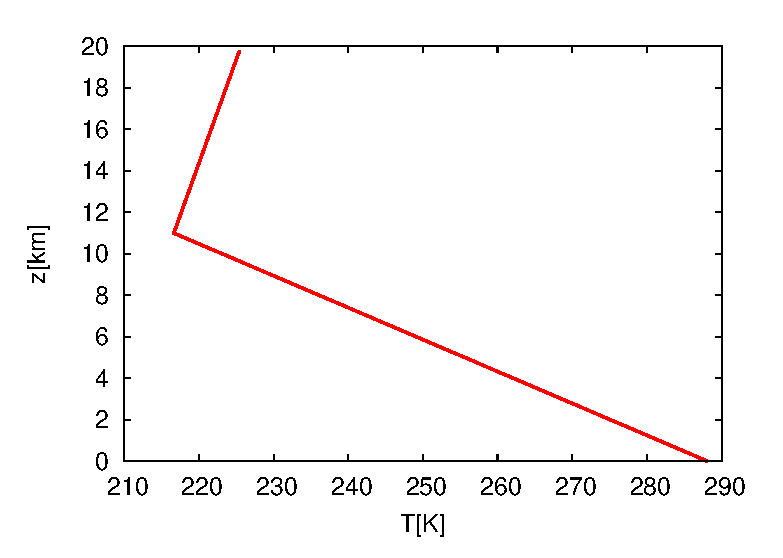
\includegraphics{./figure/us_std_atm_profile.eps}\\
  (b)\\
  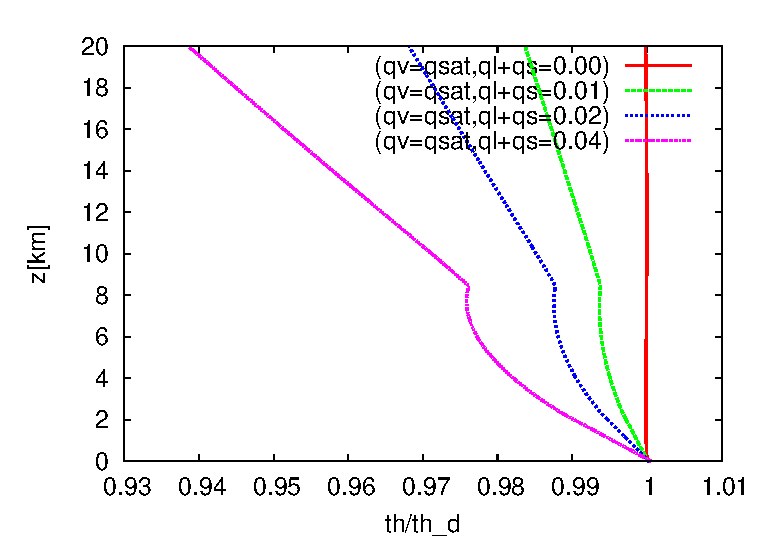
\includegraphics{./figure/theta_theta_d_profile.eps}\\
  \caption{Thee vertical profile of (a) U.S. standard atmosphere,
  (b) Several profiles of $\theta/\theta_d$.}
  \label{fig:fig1}
\end{figure}


\chapter{Discretization of dynamics}
\label{chap:discretization dynamics}
{\bf \Large
\begin{tabular}{ccc}
\hline
  Corresponding author & : & Seiya Nishizawa\\
\hline
\end{tabular}
}

\section{Temporal integration scheme}

\subsection{Runge-Kutta schemes}

For the time integration of Eqs.(\ref{eq:rhotot_d2})-(\ref{eq:etot_d2}),
we adopt the full explicit scheme with
the $p$ step Runge-Kutta scheme.
\begin{eqnarray}
&& \phi^{*}_{0} = \phi^{t}\\
&& k_1 = f(\phi^t) \\
&& k_2 = f(\phi^t + k_1 \Delta t \alpha_1) \\
&&  \cdot \cdot \cdot\nonumber\\
&& k_p = f(\phi^t + k_{p-1} \Delta t \alpha_{p-1}) \\
&& \phi^{t+\Delta t} = \phi^t + \Delta t\sum_p \beta_p k_p. \label{eq:rkscheme_last_stage}
\end{eqnarray}
The 3 and 4 step Runge-Kutta scheme are implemented.


\subsubsection{The Heun's three step scheme}

\begin{align}
  k_1 &= f(\phi^n), \\
  k_2 &= f\left(\phi^n + \frac{1}{3}\Delta t k_1\right), \\
  k_3 &= f\left(\phi^n + \frac{2}{3}\Delta t k_2\right), \\
  \phi^{n+1} &= \phi^n + \frac{1}{4}\Delta t (k_1 + 3k_3).
\end{align}


\subsubsection{The Kutta's three step scheme}

\begin{align}
  k_1 &= f(\phi^n), \\
  k_2 &= f\left(\phi^n + \frac{1}{2}\Delta t k_1\right), \\
  k_3 &= f\left(\phi^n - \Delta t k_1  + 2 \Delta t k_2\right), \\
  \phi^{n+1} &= \phi^n + \frac{1}{6}\Delta t (k_1 + 4k_2 + k_3).
\end{align}


\subsubsection{The \citet{Wicker_2002}'s three step scheme}

\begin{align}
  k_1 &= f(\phi^n), \\
  k_2 &= f\left(\phi^n + \frac{1}{3}\Delta t k_1\right), \\
  k_3 &= f\left(\phi^n + \frac{1}{2}\Delta t k_2\right), \\
  \phi^{n+1} &= \phi^n + \Delta t k_3.
\end{align}


\subsubsection{The four step scheme}

\begin{align}
  k_1 &= f(\phi^n), \\
  k_2 &= f\left(\phi^n + \frac{1}{2}\Delta t k_1\right), \\
  k_3 &= f\left(\phi^n + \frac{1}{2}\Delta t k_2\right), \\
  k_4 &= f\left(\phi^n + \Delta t k_3\right), \\
  \phi^{n+1} &= \phi^n + \frac{1}{6}\Delta t (k_1 + 2k_2 + 2k_3 + k_4).
\end{align}


\subsubsection{The forward-backward scheme}
In the short time step, the momentums are updated first and then density is updated with the updated momentums.
\begin{align}
  \rho u^{n+1}_i &= \rho u^n_i + \Delta t f_{\rho u_i}(\rho^n), \\
  \rho^{n+1}     &= \rho^n + \Delta t f_{\rho}(\rho u^{n+1}_i).
\end{align}

\subsection{Numerical stability}

A fully compressive equations of a acoustic mode is considered.
The continuous and momentum equations is the followings:
\begin{align}
  \frac{\partial \rho}{\partial t} &=
  - \frac{\partial \rho u_i}{\partial x_i} \\
  \frac{\partial \rho u_i}{\partial t} &=
  - \frac{\partial p}{\partial x_i} \\
  p &= p_0 \left( \frac{R \rho \theta}{p_0} \right)^{c_p/c_v},
\end{align}
here the potential temperature $\theta$ is assumed to be constant.

In order to analyze the numerical stability of equation, the equation of the state is linearized.
\begin{equation}
  p \approx \bar{p} + c^2 \rho',
\end{equation}
where $c$ is the sound speed: $c^2=\frac{c_p\bar{p}}{c_v\bar{\rho}}$.


We discritize the governing equation with the 2nd order central difference.
\begin{align}
  \left. \frac{\partial \rho}{\partial t}\right|_{i,j,k} &=
  -\frac{U_{i+1/2}-U_{i-1/2}}{\Delta x}
  -\frac{V_{j+1/2}-V_{j-1/2}}{\Delta y}
  -\frac{W_{k+1/2}-W_{k-1/2}}{\Delta z} \\
  \left. \frac{\partial U}{\partial t}\right|_{i+1/2} &=
  -c^2\frac{\rho_{i+1}-\rho_i}{\Delta x} \\
  \left. \frac{\partial V}{\partial t}\right|_{j+1/2} &=
  -c^2\frac{\rho_{j+1}-\rho_j}{\Delta y} \\
  \left. \frac{\partial W}{\partial t}\right|_{i+1/2} &=
  -c^2\frac{\rho_{k+1}-\rho_k}{\Delta z},
\end{align}
where $U, V$, and $W$ is the momentum at the staggared grid point in $x, y$, and $z$ direction, respectively.

The error of the spatial difference of a wavenumber $k$ component $\hat{\phi}_k$ is $\left\{\exp(ik\Delta x)-1\right\}\hat{\phi}$, and the error of 2-grid mode is the largest: $\exp(i\pi)-1 = -2$.

The temporal differential of the 2-grid mode is
\begin{align}
  \frac{\partial \rho}{\partial t} &=
  -\frac{1-\exp(-i\pi)}{\Delta x}U
  -\frac{1-\exp(-i\pi)}{\Delta y}V
  -\frac{1-\exp(-i\pi)}{\Delta z}W \\
  \frac{\partial U}{\partial t} &=
  -c^2\frac{\exp(i\pi)-1}{\Delta x}\rho \\
  \frac{\partial V}{\partial t} &=
  -c^2\frac{\exp(i\pi)-1}{\Delta y}\rho \\
  \frac{\partial W}{\partial t} &=
  -c^2\frac{\exp(i\pi)-1}{\Delta z}\rho.
\end{align}
The mode of which the $U, V$ and $W$ has the same phase is the most unstable:
\begin{align}
  \frac{\partial \rho}{\partial t} &=
  -3\frac{1-\exp(-i\pi)}{\Delta x}U \\
  \frac{\partial U}{\partial t} &=
  -c^2\frac{\exp(i\pi)-1}{\Delta x}\rho
\end{align}

Writing matrix form,
\begin{equation}
  \begin{pmatrix}
    \frac{\partial \rho}{\partial t} \\
    \frac{\partial U}{\partial t}
  \end{pmatrix}
  = D
  \begin{pmatrix}
    \rho \\
    U
  \end{pmatrix},
\end{equation}
where
\begin{equation}
  D =
  \begin{pmatrix}
    0 & -\frac{6}{\Delta x} \\
    \frac{2c^2}{\Delta x} & 0
  \end{pmatrix}.
\end{equation}

\subsubsection{The Euler scheme}
With the Euler scheme,
\begin{equation}
  \phi^{n+1} = \phi^n + \Delta t f(\phi^n)
\end{equation}
The $A$ is the matrix representing the time step, then
\begin{align}
  A &= I + dt D, \\
    &= \begin{pmatrix}
    1 & -6\frac{\Delta t}{\Delta x} \\
    \frac{2c^2\Delta t}{\Delta x} & 1
    \end{pmatrix}.
\end{align}
The eigen value of $A$ is larger than 1, and the Euler scheme is unstable for any $\Delta t$.


\subsubsection{The second step Runge-Kutta scheme}
The Heun's second step Runge-Kutta scheme is
\begin{align}
  k_1 &= f(\phi^n), \\
  k_2 &= f(\phi^n + \Delta t k_1), \\
  \phi^{n+1} &= \phi^n + \frac{\Delta t}{2}(k_1 + k_2).
\end{align}

\begin{align}
  A &= I + \frac{\Delta t}{2}(K_1 + K_2), \\
  K_1 &= D, \\
  K_2 &= D (I + \Delta t K_1).
\end{align}
After all,
\begin{equation}
  A = \begin{pmatrix}
    1-6\nu^2 & -\frac{6\Delta t}{\Delta x} \\
    \frac{2c^2\Delta t}{\Delta x} & 1-6\nu^2
    \end{pmatrix},
\end{equation}
where $\nu$ is the Courant number for the sound speed: $\frac{c\Delta t}{\Delta x}$.
The eigen value of $A$ is larger than 1, and the Euler scheme is unstable for any $\Delta t$.



\subsubsection{The third step Runge-Kutta scheme}
With the Heun's third step Runge-Kutta scheme, the matrix $A$ is written by
\begin{align}
  A &= I + \frac{\Delta t}{4}(K_1 + 4K_3), \\
  &= \begin{pmatrix}
    1-6\nu^2 & -\frac{6\Delta t}{\Delta x}(1-2\nu^2) \\
    \frac{2c^2\Delta t}{\Delta x}(1-2\nu^2) & 1-6\nu^2
  \end{pmatrix}, \label{eq: A two}
\end{align}
where
\begin{align}
  K_1 &= D, \\
  K_2 &= D (I + \frac{\Delta t}{3}K_1), \\
  K_3 &= D (I + \frac{2\Delta t}{3}K_2).
\end{align}

The condition that all the eigen values are less than or equal to 1 is
\begin{equation}
  \nu \leq \frac{1}{2}. \label{eq: cond nu two}
\end{equation}

In the Kutta's three step Runge-Kutta scheme, the matrix $A$ is
\begin{equation}
  A = I + \frac{\Delta t}{6}(K_1 + 4K_2 + K_3),
\end{equation}
where
\begin{align}
  K_1 &= D, \\
  K_2 &= D \left(I + \frac{\Delta t}{2}K_1\right), \\
  K_3 &= D \left(I - \Delta t K_1 + 2\Delta t K_2\right).
\end{align}
It is the idential as that in the Heun's scheme (eq. \ref{eq: A two}).
Thus, the stable condition is the same (eq. \ref{eq: cond nu two}).

The \citet{Wicker_2002}'s Runge-Kutta scheme is described as
\begin{align}
  A &= I + \Delta t K_3, \\
  K_1 &= D, \\
  K_2 &= D \left(I + \frac{\Delta t}{3}K_1\right), \\
  K_3 &= D \left(I + \frac{\Delta t}{2}K_2\right).
\end{align}
The $A$ and the consequent stable condition are the identical as the above two schemes.


\subsubsection{The four step Runge-Kutta scheme}
The matrix $A$ is
\begin{align}
  A &= I + \frac{\Delta t}{6}(K_1 + 2K_2 + 2K_3 + K_4), \\
  &= \begin{pmatrix}
    1-6\nu^2+6\nu^4 & -\frac{6\Delta t}{\Delta x}(1-2\nu^2) \\
    \frac{2c^2\Delta t}{\Delta x}(1-2\nu^2) & 1-6\nu^2+6^4
  \end{pmatrix},
\end{align}
where
\begin{align}
  K_1 &= D, \\
  K_2 &= D \left(I + \frac{\Delta t}{2}K_1\right), \\
  K_3 &= D \left(I + \frac{\Delta t}{2}K_2\right), \\
  K_4 &= D (I + \Delta t K_3).
\end{align}

The condition for stability is
\begin{equation}
  \nu \le \frac{\sqrt{6}}{3}.
\end{equation}

The number of floating point operations with the four step Runge-Kutta scheme is about $4/3$ times larger than that with the three step scheme.
However, the time step can be $2\sqrt{6}/3$ larger than that in the three step scheme.
Since $2\sqrt{6}/3 > 4/3$, the four step Runge-Kutta scheme is more cost effective than the three step scheme in terms of numerical stability.


\subsubsection{The forward-backward scheme}
The stability condition is
\begin{equation}
  \nu \le \frac{1}{\sqrt{3}}.
\end{equation}

The forward-backward scheme can be used in each step in the Runge-Kutta schemes.
The stability conditions are the followings:
\begin{description}
 \item[The second step RK scheme]
 \begin{equation}
   \nu \le \frac{1}{\sqrt{3}}.
 \end{equation}

 \item[The Heun's three step RK scheme]
 \begin{equation}
   \nu \le \frac{1}{2}.
 \end{equation}

 \item[The Kutta's three step RK scheme]
 \begin{equation}
   \nu \le \frac{1}{2}.
 \end{equation}

 \item[The\citet{Wicker_2002}'s three step RK scheme]
 \begin{equation}
   \nu \le \frac{\sqrt{6}}{4}.
 \end{equation}

 \item[The four step RK scheme]
 \begin{equation}
   \nu \le 0.66
 \end{equation}


\end{description}


\chapter{Descretization of the dynamics}
{\bf \Large 
\begin{tabular}{ccc}
\hline
  Corresponding author & : & Hirofumi Tomita\\
\hline
\end{tabular}
}

\section{Time integration method}

For the time integration of Eqs.(\ref{eq:rhotot_d2})-(\ref{eq:etot_d2}),
we adopt the full explicit scheme with
the $p$-th order Runge-Kutta scheme.
\begin{eqnarray}
&&  \phi^{*} = \phi^{t} - \left(\frac{\partial \phi}{\partial t}\right)^{t}\frac{\Delta t}{p}\\
&&  \phi^{**} = \phi^{t} - \left(\frac{\partial \phi}{\partial t}\right)^{*}\frac{\Delta t}{p-1}\\
&&  \cdot \cdot \cdot\nonumber\\
&&  \cdot \cdot \cdot\nonumber\\
&&  \cdot \cdot \cdot\nonumber\\
&&  \phi^{t+\Delta t} = \phi^{t} - \left(\frac{\partial \phi}{\partial t}\right)^{**\cdot\cdot\cdot\cdot*} \Delta t
\end{eqnarray}
Usually, we use $p=2,3$ and $4$.

%% HEVE full explicit
%% HEVI 
%% HIVI full implicit

\section{Spatial descretization}
We employ the Arakawa-C staggered grid with the 3-dimensional momentum 
($\rho u, \rho v, \rho w$), density ($\rho$) and mass-weighted potentail temperature($\rho \theta$)
as the prognostic variables.
Figure \ref{fig:cntrl-volume} shows the structure of the control volume for the mass,
indicating the location of each of prognostic variables.
Conceptually, we use the 4th order central difference scheme 
for the advection or convection terms and
the 2nd order central difference scheme for the other terms.
Before the descretization of differential equations,
we should diagnose several quantities from the prognostic variables.
\begin{description}
\item[Full-level pressure and potential temperature]
\begin{eqnarray}
&&p_{i,j,k}=p_{00}\left[\frac{(\rho \theta)_{i,j,k} R^*}{p_{00}} \right]^{\frac{c_{p}^*}{c_{p}^*- R^*}}\\
&&\theta_{i,j,k} = \frac{(\rho \theta)_{i,j,k}}{\rho_{i,j,k}}\\
\end{eqnarray}
\item[Half-level density]
\begin{eqnarray}
&&  \overline{\rho}_{i+\frac{1}{2},j,k} = \frac{\rho_{i+1,j,k}+\rho_{i,j,k}}{2}\\
&&  \overline{\rho}_{i,j+\frac{1}{2},k} = \frac{\rho_{i,j+1,k}+\rho_{i,j,k}}{2}\\
&&  \overline{\rho}_{i,j,k+\frac{1}{2}} = \frac{\rho_{i,j,k+1}+\rho_{i,j,k}}{2}\\
\end{eqnarray}
\item[Half-level velocity]
\begin{eqnarray}
&&  \overline{u}_{i+\frac{1}{2},j,k} = \frac{(\rho u)_{i+\frac{1}{2},j,k}}{\overline{\rho}_{i+\frac{1}{2},j,k}}\\
&&  \overline{v}_{i,j+\frac{1}{2},k} = \frac{(\rho v)_{i,j+\frac{1}{2},k}}{\overline{\rho}_{i,j+\frac{1}{2},k}}\\
&&  \overline{w}_{i,j,k+\frac{1}{2}} = \frac{(\rho w)_{i,j,k+\frac{1}{2}}}{\overline{\rho}_{i,j,k+\frac{1}{2}}}
\end{eqnarray}
\item[Full-level velocity]
\begin{eqnarray}
&&  \overline{u}_{i,j,k} = \frac{(\rho u)_{i+\frac{1}{2},j,k}+(\rho u)_{i-\frac{1}{2},j,k}}{2\rho_{i,j,k}}\\
&&  \overline{v}_{i,j,k} = \frac{(\rho v)_{i,j+\frac{1}{2},k}+(\rho v)_{i,j-\frac{1}{2},k}}{2\rho_{i,j,k}}\\
&&  \overline{w}_{i,j,k} = \frac{(\rho w)_{i,j,k+\frac{1}{2}}+(\rho w)_{i,j,k-\frac{1}{2}}}{2\rho_{i,j,k}}
\end{eqnarray}
\end{description}




\begin{figure}[t]
\begin{center}
  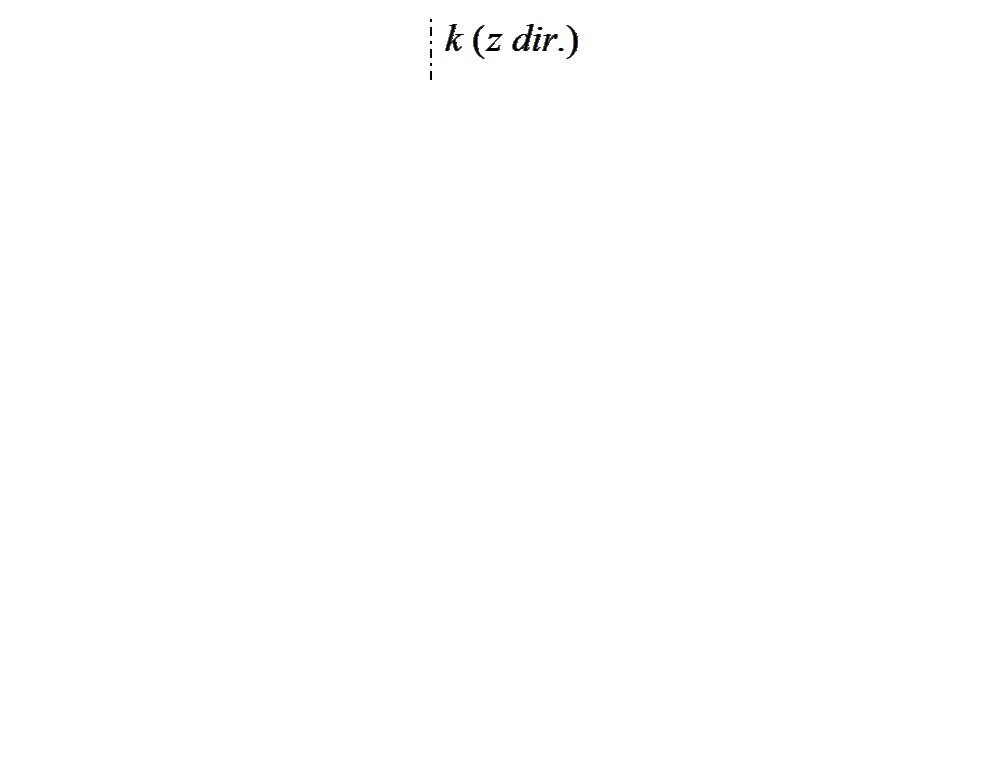
\includegraphics[scale=0.7]{./figure/cntrl-volume.eps}
\end{center}
  \caption{The control volume w.r.t. the mass}
  \label{fig:cntrl-volume}
\end{figure}


\subsection{Continuity equation}
\begin{eqnarray}
%%
\left(\frac{\partial \rho}{\partial t}\right)_{i,j,k}
&=& - \frac{(\rho u)_{i+\frac{1}{2},j,k} -(\rho u)_{i-\frac{1}{2},j,k}}{\Delta x}\nonumber\\
& & - \frac{(\rho v)_{i,j+\frac{1}{2},k} -(\rho v)_{i,j-\frac{1}{2},k}}{\Delta y}\nonumber\\
& & - \frac{(\rho w)_{i,j,k+\frac{1}{2}} -(\rho w)_{i,j,k-\frac{1}{2}}}{\Delta z}
\end{eqnarray}

\subsection{Momentum equations}
\begin{eqnarray}
%%
\left(\frac{\partial \rho u}{\partial t}\right)_{i+\frac{1}{2},j,k}
&=& - \frac{\overline{(\rho u)}_{i+1,j,k} \overline{u}_{i+1,j,k} 
           -\overline{(\rho u)}_{i,j,k} \overline{u}_{i,j,k}}
     {\Delta x}\nonumber\\
& & - \frac{\overline{(\rho u)}_{i+\frac{1}{2},j+\frac{1}{2},k}  \overline{v}_{i+\frac{1}{2},j+\frac{1}{2},k} 
           -\overline{(\rho u)}_{i+\frac{1}{2},j-\frac{1}{2},k}  \overline{v}_{i+\frac{1}{2},j-\frac{1}{2},k}}
     {\Delta y}\nonumber\\
& & - \frac{\overline{(\rho u)}_{i+\frac{1}{2},j,k+\frac{1}{2}}  \overline{v}_{i+\frac{1}{2},j,k+\frac{1}{2}} 
           -\overline{(\rho u)}_{i+\frac{1}{2},j,k-\frac{1}{2}}  \overline{v}_{i+\frac{1}{2},j,k-\frac{1}{2}}}
     {\Delta z}\nonumber\\
& & -\frac{p_{i+1,j,k}-p_{i,j,k}}{\Delta x},
\end{eqnarray}
where 
\begin{eqnarray}
&& \overline{(\rho u)}_{i,j,k} \nonumber\\
= && \frac{-(\rho u)_{i+\frac{3}{2},j,k}+7(\rho u)_{i+\frac{1}{2},j,k}+7(\rho u)_{i-\frac{1}{2},j,k}-(\rho u)_{i-\frac{3}{2},j,k}}{12}\\
&& \overline{(\rho u)}_{i+\frac{1}{2},j+\frac{1}{2},k} \nonumber\\
= && \frac{-(\rho u)_{i+\frac{1}{2},j+2,k}+7(\rho u)_{i+\frac{1}{2},j+1,k}+7(\rho u)_{i+\frac{1}{2},j,k}-(\rho u)_{i+\frac{1}{2},j-1,k}}{12}\\
&& \overline{(\rho u)}_{i+\frac{1}{2},j,k+\frac{1}{2}} \nonumber\\
= &&\frac{-(\rho u)_{i+\frac{1}{2},j,k+2}+7(\rho u)_{i+\frac{1}{2},j,k+1}+7(\rho u)_{i+\frac{1}{2},j,k}-(\rho u)_{i+\frac{1}{2},j,k-1}}{12}
\end{eqnarray}
and the velocities at the cell wall for the staggered control volume to $x$ direction are
defined as
\begin{eqnarray}
\overline{u}_{i,j,k} &=& \frac{\overline{u}_{i+\frac{1}{2},j,k}+\overline{u}_{i-\frac{1}{2},j,k}}{2}\\
\overline{v}_{i+\frac{1}{2},j+\frac{1}{2},k} &=& 
\frac{\overline{v}_{i,j+\frac{1}{2},k}+\overline{v}_{i+1,j+\frac{1}{2},k}}{2}\\
\overline{w}_{i+\frac{1}{2},j,k+\frac{1}{2}} &=& 
\frac{\overline{w}_{i,j,k+\frac{1}{2}}+\overline{w}_{i+1,j,k+\frac{1}{2}}}{2}
\end{eqnarray}
In this form, the 4th order accuracy is guaranteed 
on the condition of the constant velocity.

The momentum equations in the $y$ and $z$ directions are descretized 
in the same way:
\begin{eqnarray}
%%
\left(\frac{\partial \rho v}{\partial t}\right)_{i,j+\frac{1}{2},k}
&=& - \frac{\overline{(\rho v)}_{i+\frac{1}{2},j+\frac{1}{2},k}  \overline{u}_{i+\frac{1}{2},j+\frac{1}{2},k} 
           -\overline{(\rho v)}_{i-\frac{1}{2},j+\frac{1}{2},k}  \overline{u}_{i-\frac{1}{2},j+\frac{1}{2},k}}
     {\Delta x}\nonumber\\
& & - \frac{\overline{(\rho v)}_{i,j+1,k} \overline{v}_{i,j+1,k} 
           -\overline{(\rho v)}_{i,j,k} \overline{v}_{i,j,k}}
     {\Delta y}\nonumber\\
& & - \frac{\overline{(\rho v)}_{i,j+\frac{1}{2},k+\frac{1}{2}}  \overline{v}_{i,j+\frac{1}{2},k+\frac{1}{2}} 
           -\overline{(\rho v)}_{i,j+\frac{1}{2},k-\frac{1}{2}}  \overline{v}_{i,j+\frac{1}{2},k-\frac{1}{2}}}
     {\Delta z}\nonumber\\
& & -\frac{p_{i,j+1,k}-p_{i,j,k}}{\Delta y},\\
%%
\left(\frac{\partial \rho w}{\partial t}\right)_{i,j,k+\frac{1}{2}}
&=& - \frac{\overline{(\rho w)}_{i+\frac{1}{2},j,k+\frac{1}{2}}  \overline{u}_{i+\frac{1}{2},j,k+\frac{1}{2}} 
           -\overline{(\rho w)}_{i-\frac{1}{2},j,k+\frac{1}{2}}  \overline{u}_{i-\frac{1}{2},j,k+\frac{1}{2}}}
     {\Delta x}\nonumber\\
& & - \frac{\overline{(\rho w)}_{i,j+\frac{1}{2},k+\frac{1}{2}}  \overline{w}_{i,j+\frac{1}{2},k+\frac{1}{2}} 
           -\overline{(\rho w)}_{i,j-\frac{1}{2},k+\frac{1}{2}}  \overline{w}_{i,j-\frac{1}{2},k+\frac{1}{2}}}
     {\Delta y}\nonumber\\
& & - \frac{\overline{(\rho w)}_{i,j,k+1} \overline{w}_{i,j,k+1} 
           -\overline{(\rho w)}_{i,j,k} \overline{w}_{i,j,k}}
     {\Delta z}\nonumber\\
& & -\frac{p_{i,j,k+1}-p_{i,j,k}}{\Delta z}-\overline{\rho}_{i,j,k+\frac{1}{2}} g
\end{eqnarray}

\subsection{Energy equation}

\begin{eqnarray}
%%
\left(\frac{\partial \rho \theta}{\partial t}\right)_{i,j,k}
&=& - \frac{(\rho u)_{i+\frac{1}{2},j,k} \overline{\theta}_{i+\frac{1}{2},j,k} 
           -(\rho u)_{i-\frac{1}{2},j,k} \overline{\theta}_{i-\frac{1}{2},j,k}}
     {\Delta x}\nonumber\\
& &  - \frac{(\rho v)_{i,j+\frac{1}{2},k} \overline{\theta}_{i,j+\frac{1}{2},k} 
           -(\rho v)_{i,j-\frac{1}{2},k} \overline{\theta}_{i,j-\frac{1}{2},k}}
     {\Delta y}\nonumber\\
& &  - \frac{(\rho w)_{i,j,k+\frac{1}{2}} \overline{\theta}_{i,j,k+\frac{1}{2}} 
           -(\rho w)_{i,j,k-\frac{1}{2}} \overline{\theta}_{i,j,k-\frac{1}{2}}}
     {\Delta z}\nonumber\\
\end{eqnarray}
where
\begin{eqnarray}
&& \overline{\theta}_{i+\frac{1}{2},j,k} = 
\frac{-\theta_{i+2,j,k}+7\theta_{i+1,j,k}+7\theta_{i,j,k}-\theta_{i-1,j,k}}{12}\\
&& \overline{\theta}_{i,j+\frac{1}{2},k} = 
\frac{-\theta_{i,j+2,k}+7\theta_{i,j+1,k}+7\theta_{i,j,k}-\theta_{i,j-1,k}}{12}\\
&& \overline{\theta}_{i,j,k+\frac{1}{2}} = 
\frac{-\theta_{i,j,k+2}+7\theta_{i,j,k+1}+7\theta_{i,j,k}-\theta_{i,j,k-1}}{12}
\end{eqnarray}

\subsection{Tracer advection}
{\Huge TBD}
description of CWC and FCT. 

\section{boundary condition}
The boundary condition only for the vertical velocity at the top and bottom
boundaries is needed:
\begin{eqnarray}
&&  w_{i,j,k_{max}+\frac{1}{2}} = 0\\
&&  w_{i,j,k_{min}-\frac{1}{2}} = 0
\end{eqnarray}
This leads to the boundary condition of the prognostic variable as
\begin{eqnarray}
&&  (\rho w)_{i,j,k_{max}+\frac{1}{2}} = 0\\
&&  (\rho w)_{i,j,k_{min}-\frac{1}{2}} = 0
\end{eqnarray}



\section{Numerical filters}

We impose no explicit numerical filter.
The numerical stability can be achieved
by aid of tiny portion of turbulence scheme.


\chapter{Terrain-following Coordinates}
\label{chap:terrain-following}
{\bf \Large 
\begin{tabular}{ccc}
\hline
  Corresponding author & : & Hisashi Yashiro\\
\hline
\end{tabular}
}

\section{Geometry and Definitions}
We introduce a terrain following coordinate system with a new vertical coordinate $\xi$. 
$\xi$-coordinate system is not deformable system. We use the relation between z and $\xi$ as

\begin{eqnarray}
 \xi = \frac{z_{toa}(z-z_{sfc})}{z_{toa}-z_{sfc}},
\end{eqnarray}
Where $z_{toa}$ is the top of the model domain and $z_{sfc}$ is the surface height, 
which depends on the horizontal location.

The metrics are defined as
\begin{align}
 G^{\frac{1}{2}} &= \frac{\partial z}{\partial \xi}, \\
 \left(\frac{\partial \xi}{\partial x}\right)_{z} &= -\frac{J_{x}}{G^{\frac{1}{2}}},\\
 \left(\frac{\partial \xi}{\partial y}\right)_{z} &= -\frac{J_{y}}{G^{\frac{1}{2}}},\\
       \frac{\partial \xi}{\partial z}            &=  \frac{1}{G^{\frac{1}{2}}},
\end{align}
where
\begin{align}
 J_{x} &= \left(\frac{\partial z}{\partial x}\right)_{\xi},\\
 J_{y} &= \left(\frac{\partial z}{\partial y}\right)_{\xi}.
\end{align}

If we use the Eqs.(5.2)-(5.5), we obtain following equations:
\begin{align}
 \nabla \cdot (G^{\frac{1}{2}} \phi) &= \left(\frac{\partial G^{\frac{1}{2}} \phi}{\partial x}\right)_{\xi}
                                      + \left(\frac{\partial G^{\frac{1}{2}} \phi}{\partial y}\right)_{\xi}
                                      + \frac{(J_{x}+J_{y}-1)}{G^{\frac{1}{2}}} \frac{\partial G^{\frac{1}{2}} \phi}{\partial \xi}, \\
 \nabla \cdot (G^{\frac{1}{2}} \bf u) &= \frac{\partial G^{\frac{1}{2}} u}{\partial x}
                                       + \frac{\partial G^{\frac{1}{2}} v}{\partial y}
                                       + \frac{1}{G^{\frac{1}{2}}} \frac{\partial}{\partial \xi}
                                         \left(J_{x} {G^{\frac{1}{2}}} u+J_{y} {G^{\frac{1}{2}}} v - {G^{\frac{1}{2}}} w\right).
\end{align}

\section{Summary of modified equations in the dynamical process}

We change prognostic variables by multiplying $G^{\frac{1}{2}}$ as
\begin{align}
 (\rho Q_v)_{i,j,k}           &= G^{\frac{1}{2}}_{i,j,k}             (\rho Q_v)_{i,j,k},        \\
 (\rho Q_l)_{i,j,k}           &= G^{\frac{1}{2}}_{i,j,k}             (\rho Q_l)_{i,j,k},        \\
 (\rho Q_s)_{i,j,k}           &= G^{\frac{1}{2}}_{i,j,k}             (\rho Q_s)_{i,j,k},        \\
 R_{i,j,k}                    &= G^{\frac{1}{2}}_{i,j,k}              \rho_{i,j,k},                \\
 (\rho U)_{i+\frac{1}{2},j,k} &= G^{\frac{1}{2}}_{i+\frac{1}{2},j,k} (\rho u)_{i+\frac{1}{2},j,k}, \\
 (\rho V)_{i,j+\frac{1}{2},k} &= G^{\frac{1}{2}}_{i,j+\frac{1}{2},k} (\rho v)_{i,j+\frac{1}{2},k}, \\
 (\rho W)_{i,j,k+\frac{1}{2}} &= G^{\frac{1}{2}}_{i,j,k+\frac{1}{2}} (\rho w)_{i,j,k+\frac{1}{2}}, \\
 (\rho \Theta)_{i,j,k}        &= G^{\frac{1}{2}}_{i,j,k}             (\rho \theta)_{i,j,k},        \\
 P_{i,j,k}                    &= G^{\frac{1}{2}}_{i,j,k}              p_{i,j,k}
\end{align}

and Eqs.(2.67)-(2.72) are modified using Eqs.(5.2)-(5.5).

\begin{align}
 \frac{\partial \rho Q_v     }{\partial t} + \nabla \cdot \left( \rho Q_v             {\bf u}\right) &= 0 \\
 \frac{\partial \rho Q_l     }{\partial t} + \nabla \cdot \left( \rho Q_l             {\bf u}\right) &= 0 \\
 \frac{\partial \rho Q_s     }{\partial t} + \nabla \cdot \left( \rho Q_s             {\bf u}\right) &= 0 \\
 \frac{\partial R            }{\partial t} + \nabla \cdot \left( R                    {\bf u}\right) &= 0 \\
 \frac{\partial \rho {\bf U} }{\partial t} + \nabla \cdot \left( \rho {\bf U} \otimes {\bf u}\right) &= -\nabla P - Rg {\bf e_z} \\
 \frac{\partial \rho \Theta  }{\partial t} + \nabla \cdot \left( \rho \Theta          {\bf u}\right) &= 0
\end{align}

\section{Spatial descretization}
\subsection{Continuity equation}
\begin{align}
 \left(\frac{\partial R}{\partial t}\right)_{i,j,k}
 = - G^{\frac{1}{2}}_{i,j,k} &\Bigg[ \frac{ (\rho u)_{i+\frac{1}{2},j,k}
                                          - (\rho u)_{i-\frac{1}{2},j,k}
                                          } {\Delta x} \nonumber \\
                                  &+ \frac{ (\rho v)_{i,j+\frac{1}{2},k}
                                          - (\rho v)_{i,j-\frac{1}{2},k}
                                          } {\Delta y} \nonumber \\
                                  &+ \frac{ (J_{x})_{i,j,k+\frac{1}{2}} \overline{\overline{(\rho u)}}^z_{i,j,k+\frac{1}{2}}
                                          - (J_{x})_{i,j,k-\frac{1}{2}} \overline{\overline{(\rho u)}}^z_{i,j,k-\frac{1}{2}}
                                          } {\Delta \xi} \nonumber \\
                                  &+ \frac{ (J_{y})_{i,j,k+\frac{1}{2}} \overline{\overline{(\rho v)}}^z_{i,j,k+\frac{1}{2}}
                                          - (J_{y})_{i,j,k-\frac{1}{2}} \overline{\overline{(\rho v)}}^z_{i,j,k-\frac{1}{2}}
                                          } {\Delta \xi} \nonumber \\
                                  &+ \frac{ (\rho w)_{i,j,k+\frac{1}{2}}
                                          - (\rho w)_{i,j,k-\frac{1}{2}}
                                          } {\Delta \xi} \Bigg]
\end{align}
where
\begin{align}
 \overline{\overline{(\rho u)}}^z_{i,j,k+\frac{1}{2}} &= \frac{ \overline{(\rho u)}_{i,j,k+1}
                                                              + \overline{(\rho u)}_{i,j,k  }
                                                              } {2}, \\
 \overline{\overline{(\rho v)}}^z_{i,j,k+\frac{1}{2}} &= \frac{ \overline{(\rho v)}_{i,j,k+1}
                                                              + \overline{(\rho v)}_{i,j,k  }
                                                              } {2},
\end{align}
$\overline{(\rho u)}_{i,j,k}$ and $\overline{(\rho v)}_{i,j,k}$ are obtained by same manner in eq.(3.20)

\subsection{Momentum equations}
\begin{align}
 \left(\frac{\partial \rho U}{\partial t}\right)_{i+\frac{1}{2},j,k}
 = - &\Bigg[ \frac{ \overline{(\rho U)}_{i+1,j,k} \overline{u}_{i+1,j,k}
                  - \overline{(\rho U)}_{i  ,j,k} \overline{u}_{i  ,j,k}
                  } {\Delta x} \nonumber \\
          &+ \frac{ \overline{(\rho U)}_{i+\frac{1}{2},j+\frac{1}{2},k} \overline{v}_{i+\frac{1}{2},j+\frac{1}{2},k}
                  - \overline{(\rho U)}_{i+\frac{1}{2},j-\frac{1}{2},k} \overline{v}_{i+\frac{1}{2},j-\frac{1}{2},k}
                  } {\Delta y} \nonumber \\
          &- \frac{1}{\Delta \xi} \Bigg( \overline{(\rho U)}_{i+\frac{1}{2},j,k+\frac{1}{2}} (-(J_{x}) \overline{\overline{u}}^{z} -(J_{y}) \overline{\overline{v}}^{xz} + \overline{w})_{i+\frac{1}{2},j,k+\frac{1}{2}} \nonumber \\
                                      &- \overline{(\rho U)}_{i+\frac{1}{2},j,k-\frac{1}{2}} (-(J_{x}) \overline{\overline{u}}^{z} -(J_{y}) \overline{\overline{v}}^{xz} + \overline{w})_{i+\frac{1}{2},j,k-\frac{1}{2}} \Bigg) \nonumber \\
          &+ \frac{ P_{i+1,j,k}-P_{i,j,k}}{\Delta x} \nonumber \\
          &+ \frac{ (J_{x})_{i+\frac{1}{2},j,k+\frac{1}{2}} \overline{p}^{xz}_{i+\frac{1}{2},j,k+\frac{1}{2}}
                  - (J_{x})_{i+\frac{1}{2},j,k-\frac{1}{2}} \overline{p}^{xz}_{i+\frac{1}{2},j,k-\frac{1}{2}}
                  } {\Delta \xi},
\end{align}

where $\overline{(\rho U)}_{i,j,k}$, $\overline{(\rho U)}_{i+\frac{1}{2},j+\frac{1}{2},k}$ 
and $\overline{(\rho U)}_{i+\frac{1}{2},j,k+\frac{1}{2}}$ is obtained according to the method of eq(3.20)-(3.22).
The velocities at the cell wall for the staggered control volume to x direction are defined by eq(3.23)-(3.25).
$\overline{\overline{u}}^z$ and $\overline{\overline{v}}^{xz}$ are defined as

\begin{align}
 \overline{\overline{u}}^z_{i+\frac{1}{2},j,k+\frac{1}{2}}    &= \frac{ \overline{u}_{i+\frac{1}{2},j,k+1}
                                                                      + \overline{u}_{i+\frac{1}{2},j,k  }
                                                                      } {2}, \\
 \overline{\overline{v}}^{xz}_{i+\frac{1}{2},j,k+\frac{1}{2}} &= \frac{ \overline{v}_{i+1,j,k+1}
                                                                      + \overline{v}_{i+1,j,k  }
                                                                      + \overline{v}_{i  ,j,k+1}
                                                                      + \overline{v}_{i  ,j,k  }
                                                                      } {4}.
\end{align}

$\overline{p}^{xz}$ is defined as
\begin{align}
 \overline{\overline{p}}^{xz}_{i+\frac{1}{2},j,k+\frac{1}{2}} &= \frac{ \overline{p}_{i+1,j,k+1}
                                                                      + \overline{p}_{i+1,j,k  }
                                                                      + \overline{p}_{i  ,j,k+1}
                                                                      + \overline{p}_{i  ,j,k  }
                                                                      } {4}.
\end{align}

The momentum equations in the $y$ and $z$ directions are descretized 
in the same way:
\begin{align}
 \left(\frac{\partial \rho V}{\partial t}\right)_{i,j+\frac{1}{2},k}
 = - &\Bigg[ \frac{ \overline{(\rho V)}_{i+\frac{1}{2},j+\frac{1}{2},k} \overline{u}_{i-\frac{1}{2},j+\frac{1}{2},k}
                  - \overline{(\rho V)}_{i+\frac{1}{2},j+\frac{1}{2},k} \overline{u}_{i-\frac{1}{2},j+\frac{1}{2},k}
                  } {\Delta x} \nonumber \\
          &+ \frac{ \overline{(\rho V)}_{i,j+1,k} \overline{v}_{i,j+1,k}
                  - \overline{(\rho V)}_{i,j  ,k} \overline{v}_{i,j  ,k}
                  } {\Delta y} \nonumber \\
          &- \frac{1}{\Delta \xi} \Bigg( \overline{(\rho V)}_{i,j+\frac{1}{2},k+\frac{1}{2}} (-(J_{x}) \overline{\overline{u}}^{yz} -(J_{y}) \overline{\overline{v}}^{z} + \overline{w})_{i,j+\frac{1}{2},k+\frac{1}{2}} \nonumber \\
                                      &- \overline{(\rho V)}_{i,j+\frac{1}{2},k-\frac{1}{2}} (-(J_{x}) \overline{\overline{u}}^{yz} -(J_{y}) \overline{\overline{v}}^{z} + \overline{w})_{i,j+\frac{1}{2},k-\frac{1}{2}} \Bigg) \nonumber \\
          &+ \frac{ P_{i,j+1,k}-P_{i,j,k}}{\Delta y} \nonumber \\
          &+ \frac{ (J_{y})_{i,j+\frac{1}{2},k+\frac{1}{2}} \overline{p}^{yz}_{i,j+\frac{1}{2},k+\frac{1}{2}}
                  - (J_{y})_{i,j+\frac{1}{2},k-\frac{1}{2}} \overline{p}^{yz}_{i,j+\frac{1}{2},k-\frac{1}{2}}
                  } {\Delta \xi}, \\
 \left(\frac{\partial \rho W}{\partial t}\right)_{i,j,k+\frac{1}{2}}
 = - &\Bigg[ \frac{ \overline{(\rho W)}_{i+\frac{1}{2},j,k+\frac{1}{2}} \overline{u}_{i+\frac{1}{2},j,k+\frac{1}{2}}
                  - \overline{(\rho W)}_{i-\frac{1}{2},j,k+\frac{1}{2}} \overline{u}_{i-\frac{1}{2},j,k+\frac{1}{2}}
                  } {\Delta x} \nonumber \\
          &+ \frac{ \overline{(\rho W)}_{i,j+\frac{1}{2},k+\frac{1}{2}} \overline{v}_{i,j+\frac{1}{2},k+\frac{1}{2}}
                  - \overline{(\rho W)}_{i,j-\frac{1}{2},k+\frac{1}{2}} \overline{v}_{i,j-\frac{1}{2},k+\frac{1}{2}}
                  } {\Delta y} \nonumber \\
          &+ \frac{1}{\Delta \xi} \Bigg( \overline{(\rho W)}_{i,j,k+1} (-(J_{x}) \overline{u} -(J_{y}) \overline{v} + \overline{w})_{i,j,k+1} \nonumber \\
                                      &- \overline{(\rho W)}_{i,j,k  } (-(J_{x}) \overline{u} -(J_{y}) \overline{v} + \overline{w})_{i,j,k  } \Bigg) \nonumber \\
          &- \frac{ p_{i,j,k+1}
                  - p_{i,j,k  }
                  } {\Delta \xi},
\end{align}

\subsection{Energy equation}

\begin{align}
 \left(\frac{\partial \rho \Theta}{\partial t}\right)_{i,j,k}
 = - G^{\frac{1}{2}}_{i,j,k} &\Bigg[ \frac{ (\rho u)_{i+\frac{1}{2},j,k} \overline{\Theta}_{i+\frac{1}{2},j,k}
                                          - (\rho u)_{i-\frac{1}{2},j,k} \overline{\Theta}_{i-\frac{1}{2},j,k}
                                          } {\Delta x} \nonumber \\
                                  &+ \frac{ (\rho v)_{i,j+\frac{1}{2},k} \overline{\Theta}_{i,j+\frac{1}{2},k}
                                          - (\rho v)_{i,j-\frac{1}{2},k} \overline{\Theta}_{i,j-\frac{1}{2},k}
                                          } {\Delta y} \nonumber \\
                                  &+ \frac{ (J_{x})_{i,j,k+\frac{1}{2}} \overline{\overline{(\rho u)}}^z_{i,j,k+\frac{1}{2}} \overline{\Theta}_{i,j,k+\frac{1}{2}}
                                          - (J_{x})_{i,j,k-\frac{1}{2}} \overline{\overline{(\rho u)}}^z_{i,j,k-\frac{1}{2}} \overline{\Theta}_{i,j,k-\frac{1}{2}}
                                          } {\Delta \xi} \nonumber \\
                                  &+ \frac{ (J_{y})_{i,j,k+\frac{1}{2}} \overline{\overline{(\rho v)}}^z_{i,j,k+\frac{1}{2}} \overline{\Theta}_{i,j,k+\frac{1}{2}}
                                          - (J_{y})_{i,j,k-\frac{1}{2}} \overline{\overline{(\rho v)}}^z_{i,j,k-\frac{1}{2}} \overline{\Theta}_{i,j,k-\frac{1}{2}}
                                          } {\Delta \xi} \nonumber \\
                                  &+ \frac{ (\rho w)_{i,j,k+\frac{1}{2}} \overline{\Theta}_{i,j,k+\frac{1}{2}}
                                          - (\rho w)_{i,j,k-\frac{1}{2}} \overline{\Theta}_{i,j,k-\frac{1}{2}}
                                          } {\Delta \xi} \Bigg]
\end{align}
where $\overline{\theta}_{i+\frac{1}{2},j,k}$, $\overline{\theta}_{i,j+\frac{1}{2},k}$ and 
$\overline{\theta}_{i,j,k+\frac{1}{2}}$ are is obtained according to the method of eq(3.29)-(3.31).


%\documentclass{book}
%\usepackage{amsmath}
%\usepackage{bm}
%\begin{document}

\chapter{Map factor}
\label{chap: map factor}
{\bf \Large 
\begin{tabular}{ccc}
\hline
  Corresponding author & : & Seiya Nishizawa\\
\hline
\end{tabular}
}

\newcommand{\pd}[2]{\frac{\partial #1}{\partial #2}}


\section{Coordinate transform}
A orthogonal rectangular coordinate $(x, y, z)$.
A orthogonal curvilinear coordinate $(\xi, \eta, \zeta)$.


The transform is defined by
\begin{align}
  \bm{e}_\xi &= \pd{x}{\xi}\bm{e}_x + \pd{y}{\xi}\bm{e}_y + \pd{z}{\xi}\bm{e}_z, \\
  \bm{e}_\eta &= \pd{x}{\eta}\bm{e}_x + \pd{y}{\eta}\bm{e}_y + \pd{z}{\eta}\bm{e}_z, \\
  \bm{e}_\zeta &= \pd{x}{\zeta}\bm{e}_x + \pd{y}{\zeta}\bm{e}_y + \pd{z}{\zeta}\bm{e}_z.
\end{align}
Reverse transform is
\begin{align}
  \bm{e}_x &= \pd{\xi}{x}\bm{e}_\xi + \pd{\eta}{x}\bm{e}_\eta + \pd{\zeta}{x}\bm{e}_\zeta, \\
  \bm{e}_y &= \pd{\eta}{y}\bm{e}_\xi + \pd{\eta}{y}\bm{e}_\eta + \pd{\zeta}{y}\bm{e}_\zeta, \\
  \bm{e}_z &= \pd{\zeta}{z}\bm{e}_\xi + \pd{\eta}{z}\bm{e}_\eta + \pd{\zeta}{z}\bm{e}_\zeta.
\end{align}

The Jacobian matrix is $\{\pd{\xi^k}{x^i}\}$.


The reverse transform after the transform of the transform after the reverse transform make a vector to the original vector;
\begin{align}
  \pd{\xi^k}{x^i}\pd{x^i}{\xi^l} &= \delta_l^k, \\
  \pd{x^i}{\xi^k}\pd{\xi^k}{x^j} &= \delta_j^i,
\end{align}
where index which appares upper and lower suffix in a single term implies summation of the term over set ${1,2,3}$ (Einstein notation).


Spatial parial derivative is tranformed with the Jacobian matrix (covariant transform);
\begin{align}
  \pd{}{\xi^k} &= \pd{x^i}{\xi^k}\pd{}{x^i}, \\
  \pd{}{x^i} &= \pd{\xi^k}{x^i}\pd{}{\xi^k}.
\end{align}


Velocity is transformed with the inverse of the Jacobian matrix (cotravariant transform);
\begin{align}
  d\xi^k &= \pd{\xi^k}{x^i} dx^i, \\
  dx^i &= \pd{x^i}{\xi^k} d\xi^k.
\end{align}



The metric tensor, $g_{kl}$ is defined by
\begin{equation}
  g_{kl} = \bm{e}_k \cdot \bm{e}_l
  = \left(\pd{x^i}{\xi_k}\bm{e}_i\right) \cdot \left(\pd{x^j}{\xi_l}\bm{e}_j\right)
  = \pd{x^i}{\xi_k}\pd{x^j}{\xi_l} (\bm{e}_i\cdot\bm{e}_j).
\end{equation}

For orthogonal curvilinear coordinates, the matrix ${g_{kl}}$ is diagonal.
Metric factor, $h_k$ is defined as
\begin{equation}
  h_k^2 = g_{kk} = \sum_i \left(\pd{x^i}{\xi_k}\right)^2.
\end{equation}

Here we define the matrix, $\bm{E}_\xi$ is
\begin{equation}
  \bm{E}_\xi =
  (\bm{e}_\xi \bm{e}_\eta \bm{e}_\zeta)\cdot \bm{H}^{-1}
  = \bm{E}_x \cdot \left\{\pd{x^i}{\xi^k}\right\} \cdot \bm{H}^{-1},
\end{equation}
where $\bm{E}_x = (\bm{e}_x \bm{e}_y \bm{e}_z)$, and
\begin{equation}
  \bm{H} = \left(\begin{array}{ccc} h_1 & 0 & 0\\ 0 & h_2 & 0\\ 0 & 0 & h_3\end{array}\right).
\end{equation}
The vector $\frac{1}{h_k}\bm{e}_k$ is unit vector and orthogonal each other,
so the inverse of the $\bm{E}_\xi$ is $\bm{E}_\xi^T$.
\begin{align}
  \left( \bm{E}_x \cdot \left\{\pd{x^i}{\xi^k}\right\} \cdot \bm{H}^{-1} \right)^{-1} &= \left( \bm{E}_x \cdot \left\{\pd{x^i}{\xi^k}\right\} \cdot \bm{H}^{-1} \right)^T, \nonumber\\
  \bm{H} \cdot \left\{\pd{\xi^k}{x^i}\right\} \cdot \bm{E}_x^{-1} &= \bm{H}^{-1} \cdot \left\{\pd{x^i}{\xi^k}\right\}^T \cdot \bm{E}_x^T, \nonumber
\end{align}
\begin{align}
  \left\{\pd{\xi^k}{x^i}\right\} &= \bm{H}^{-2} \cdot \left\{\pd{x^i}{\xi^k}\right\}^T \cdot \bm{E}_x^T \cdot \bm{E}_x \nonumber \\
  &= \bm{H}^{-2} \cdot \left\{\pd{x^i}{\xi^k}\right\}^T.
\end{align}
That is
\begin{equation}
  \pd{\xi^k}{x^i} = \frac{1}{h_k^2} \pd{x^i}{\xi^k}.
\end{equation}


\section{Governing equations}

\subsection{Continuous equiation}

Divergence of $\rho \bm{u}$ is
\begin{align}
  \pd{}{x^i}(\rho dx^i)
  &= \pd{\xi^k}{x^i}\pd{}{\xi^k}\left(\rho \pd{x^i}{\xi^l}d\xi^l\right) \nonumber \\
  &= \pd{\xi^k}{x^i}\pd{x^i}{\xi^l}\pd{}{\xi^k}(\rho d\xi^l)
    +\rho d\xi^l \pd{\xi^k}{x^i} \frac{\partial^2 x^i}{\partial \xi^k \partial \xi^l} \nonumber\\
  &= \pd{}{\xi^k} (\rho d\xi^k) + \sum_k\frac{1}{h_k^2}\rho d\xi^l \pd{x^i}{\xi^k}\frac{\partial^2 x^i}{\partial \xi^k \partial \xi^l} \nonumber\\
  &= \pd{}{\xi^k} (\rho d\xi^k) + \sum_k \frac{1}{2h_k^2}\rho d\xi^l \pd{}{\xi^l}\left(\pd{x^i}{\xi^k}\right)^2 \nonumber\\
  &= \pd{}{\xi^k} (\rho d\xi^k) + \sum_k \frac{1}{2h_k^2}\rho d\xi^l \pd{}{\xi^l}h_k^2 \nonumber\\
  &= \pd{}{\xi^k} (\rho d\xi^k) + \sum_k \frac{1}{2}\rho d\xi^l \pd{}{\xi^l}\ln h_k^2 \nonumber\\
  &= \pd{}{\xi^k} (\rho d\xi^k) + \rho d\xi^k \pd{}{\xi^k}\ln (\prod_l h_l) \nonumber\\
  &= J \left\{ J^{-1}\pd{}{\xi^k} (\rho d\xi^l) + \rho d\xi^k \pd{}{\xi^k}J^{-1}\right\} \nonumber\\
  &= J \pd{}{\xi^k} (J^{-1}\rho d\xi^k),
\end{align}
where $J$ is the Jacobian of the Jacobian matrix and
\begin{equation}
  J = \frac{1}{\prod_k h_k}.
\end{equation}

The continuous equation is
\begin{equation}
\pd{\rho}{t} + J \pd{}{\xi^k}\frac{\rho d\xi^k}{J} = 0.
\end{equation}



\subsection{Momentum equation}

\begin{equation}
  \pd{\rho d\xi^k}{t} = \pd{\xi^k}{x^i} \pd{\rho dx^i}{t}.
\end{equation}

\begin{description}

\item[Advection term]
\begin{align}
  & \pd{\xi^k}{x^i}\pd{\rho dx^idx^j}{x^j} \nonumber\\
  &= \pd{\xi^k}{x^i}\left(dx^j\pd{\rho dx^i}{x^j} + \rho dx^i\pd{dx^j}{x^j}\right) \nonumber\\
  &= \pd{\xi^k}{x^i}\left(\pd{x^j}{\xi^l}d\xi^l\right)\pd{\xi^m}{x^j}\pd{}{\xi^m}\left(\rho \pd{x^i}{\xi^n}d\xi^n\right)
  + \pd{\xi^k}{x^i}\rho \left(\pd{x^i}{\xi^l}d\xi^l\right)\pd{\xi^m}{x^j}\pd{}{\xi^m}\left(\pd{x^j}{\xi^n}d\xi^n\right) \nonumber\\
  &= d\xi^l\pd{\xi^k}{x^i}\pd{}{\xi^l}\left(\rho \pd{x^i}{\xi^n}d\xi^n\right)
  + \rho d\xi^k\pd{\xi^m}{x^j}\pd{}{\xi^m}\left(\pd{x^j}{\xi^n}d\xi^n\right) \nonumber\\
  &= d\xi^l\pd{\xi^k}{x^i}\left\{\pd{x^i}{\xi^n}\pd{}{\xi^l}\left(\rho d\xi^n\right) + \rho d\xi^n \frac{\partial^2 x^i}{\partial \xi^l \partial \xi^n}\right\}
  + \rho d\xi^k\pd{\xi^m}{x^j} \left( \pd{x^j}{\xi^n}\pd{d\xi^n}{\xi^m} + d\xi^n\frac{\partial^2 x^j}{\partial \xi^m \partial \xi^n} \right) \nonumber\\
  &= d\xi^l\pd{}{\xi^l}\left(\rho d\xi^k\right) + \rho d\xi^l d\xi^n\pd{\xi^k}{x^i} \frac{\partial^2 x^i}{\partial \xi^l \partial \xi^n}
  + \rho d\xi^k\pd{d\xi^m}{\xi^m} + \rho d\xi^kd\xi^n\pd{\xi^m}{x^j}\frac{\partial^2 x^j}{\partial \xi^m \partial \xi^n} \nonumber\\
  &= \pd{}{\xi^l}\left(\rho d\xi^k d\xi^l\right) + \rho d\xi^l d\xi^n\pd{\xi^k}{x^i} \frac{\partial^2 x^i}{\partial \xi^l \partial \xi^n}
   + \rho d\xi^kd\xi^l\pd{\xi^m}{x^i}\frac{\partial^2 x^i}{\partial \xi^l \partial \xi^m} \nonumber\\
  &= J\left\{ J^{-1}\pd{}{\xi^l}(\rho d\xi^k d\xi^l) + \rho d\xi^k d\xi^l\pd{J^{-1}}{\xi^l} \right\}
   + \rho d\xi^ld\xi^m\pd{\xi^k}{x^i}\frac{\partial^2 x^i}{\partial \xi^l \partial \xi^m} \nonumber\\
  &= J \pd{}{\xi^l}{J^{-1}\rho d\xi^k d\xi^l} + \rho d\xi^l d\xi^m\Gamma^k_{lm},
\end{align}
where $\Gamma$ is the Christoffel symbols of the second kind, and
\begin{align}
  \Gamma_{lm}^k
  &= \pd{\xi^k}{x^i} \frac{\partial^2 x^i}{\partial \xi^l \partial \xi^m} \nonumber\\
  &= \frac{1}{2}g^{kn}\left( \pd{g_{mn}}{\xi^l} + \pd{g_{ln}}{\xi^m} - \pd{g_{lm}}{\xi^n}\right) \nonumber\\
  &= \frac{1}{h_k^2}\left( h_k\pd{h_k}{\xi^l}\delta_{km}+h_k\pd{h_k}{\xi^m}\delta_{kl}-h_l\pd{h_l}{\xi^k}\delta_{lm}\right),
\end{align}
where $\{g^{kn}\}$ is inverse matrix of $\{g_{kn}\}$.


\item[Coriolis term]
\begin{align}
  \pd{\xi^k}{x^i} \epsilon^{ijp} f^j \rho dx^p
  &= \epsilon^{klm} \frac{1}{h_kh_lh_m}\hat{f}^l d\xi^m,
\end{align}
where $\epsilon$ is the Levi-Civita symbol,
and
\begin{equation}
  \hat{f}^l = \pd{\xi^l}{x^j} f^j.
\end{equation}

\item[Pressure gradient term]
\begin{align}
  \pd{\xi^k}{x^i} \pd{p}{x^i}
  &= \pd{\xi^k}{x^i}\left(\pd{\xi^l}{x^i}\pd{p}{\xi^l}\right)\nonumber\\
  &= \frac{1}{h_k^2}\pd{x^i}{\xi^k}\pd{\xi^l}{x^i}\pd{p}{\xi^l} \nonumber\\
  &= \frac{1}{h_k^2}\pd{p}{\xi^k}.
\end{align}

\end{description}

After all, momentum equation is
\begin{align}
  \pd{}{t} \rho d\xi^k + J\pd{}{\xi^l} \left( J^{-1} \rho d\xi^k d\xi^l \right)
  + \rho d\xi^l d\xi^m \Gamma_{lm}^k
  + \epsilon^{klm} \frac{1}{h_kh_lh_m}\hat{f}^l \rho d\xi^m = -\frac{1}{h_k^2}\pd{p}{\xi^k} + \rho g^p \pd{\xi^k}{x^p}.
\end{align}



\section{Map factor}
We introduce Map factor $m, n$.
\begin{align}
  \frac{1}{m}\frac{a+z}{a} &= h_1, \\
  \frac{1}{n}\frac{a+z}{a} &= h_2, \\
  1 &= h_3,
\end{align}
where is $a$ is radius of the planet.
Assuming shallow atmospher,
\begin{align}
  m &= h_1, \\
  n &= h_2.
\end{align}

Normalized velocity is defined as
\begin{align}
  \hat{u} &= h_1\frac{d \xi}{dt} = \frac{1}{m}\frac{d \xi}{dt}, \\
  \hat{v} &= h_2\frac{d \eta}{dt} = \frac{1}{n}\frac{d \eta}{dt}, \\
  \hat{w} &= h_3\frac{d \zeta}{dt} = \frac{d \zeta}{dt}.
\end{align}

The continuous equation becomes
\begin{equation}
  \pd{\rho}{t} + mn\pd{}{\xi}\frac{\rho \hat{u}}{n} + mn\pd{}{\eta}\frac{\rho \hat{v}}{m} + \pd{}{\zeta}\rho \hat{w} = 0
\end{equation}

The momentum equations are
\begin{equation}
  \pd{\rho\hat{u}^k}{t}
  + mn\pd{}{\xi}\frac{\rho \hat{u} \hat{u}^k}{n}
  + mn\pd{}{\eta}\frac{\rho \hat{v} \hat{u}^k}{m}
  + \pd{}{\zeta}\rho \hat{w} \hat{u}^k
  + m m_k \rho \hat{u} \hat{u}^k \pd{}{\xi}\frac{1}{m_k}
  + n m_k \rho \hat{v} \hat{u}^k \pd{}{\eta}\frac{1}{m_k}
  - m m_k \rho \hat{u}^2 \pd{}{\xi^k}\frac{1}{m}
  - n m_k \rho \hat{v}^2 \pd{}{\xi^k}\frac{1}{n}
  + \epsilon^{klm} m_l \hat{f}^l \rho \hat{u}^m
  = -m_k \pd{p}{\zeta^k} + \rho g \delta_{3k}
\end{equation}

\begin{align}
  \pd{\rho u}{t} &+ mn\pd{}{\xi}\frac{\rho uu}{n} + mn\pd{}{\eta}\frac{\rho uv}{m} + \pd{}{\zeta}\rho uw \\
  &- f\rho v - mn \rho v\left\{v\pd{}{\xi}\left(\frac{1}{n}\right) - u\pd{}{\eta}\left(\frac{1}{m}\right)\right\} = -m\pd{p}{\xi}, \\
  \pd{\rho v}{t} &+ mn\pd{}{\xi}\frac{\rho uv}{n} + mn\pd{}{\eta}\frac{\rho vv}{m} + \pd{}{\zeta}\rho vw \\
  &+f\rho u + mn \rho u\left\{v\pd{}{\xi}\left(\frac{1}{n}\right) - u\pd{}{\eta}\left(\frac{1}{m}\right)\right\} = -n\pd{p}{\eta}, \\
  \pd{\rho w}{t} &+ mn\pd{}{\xi}\frac{\rho uw}{n} + mn\pd{}{\eta}\frac{\rho vw}{m} + \pd{}{\zeta}\rho ww = -\pd{p}{\zeta} -\rho g.
\end{align}

The thermodynamical and tracer equations
\begin{equation}
  \pd{\rho \phi}{t} + mn\pd{}{\xi}\frac{\rho \hat{u}\phi}{n} + mn\pd{}{\eta}\frac{\rho \hat{v}\phi}{m} + \pd{\rho \hat{w}\phi}{\zeta} = 0.
\end{equation}


%\end{document}


\chapter{Horizontal explicit virtical implicit}
\label{chap:hevi}
{\bf \Large 
\begin{tabular}{ccc}
\hline
  Corresponding author & : & Seiya Nishizawa\\
\hline
\end{tabular}
}

\section{Equations}

\begin{align}
  \frac{\partial \rho}{\partial t}
  &= -\frac{\partial \rho w}{\partial z} + S_\rho, \\
  \frac{\partial \rho w}{\partial t}
  &= -\frac{\partial p}{\partial z} -\rho g + S_{\rho w}, \\
  \frac{\partial \rho\theta}{\partial t}
  &= \frac{\partial \rho w\theta}{\partial z} + S_{\rho\theta}, \\
  p &= P_{00}\left(\frac{R\rho\theta}{P_{00}}\right)^{c_p/c_v},
\end{align}
where
\begin{align}
  S_\rho &= - \frac{\partial \rho u}{\partial x}
           - \frac{\partial \rho v}{\partial y}, \\
  S_{\rho w} &= - \frac{\partial u\rho w}{\partial x}
              - \frac{\partial v\rho w}{\partial y}
              - \frac{\partial w\rho w}{\partial z}, \\
  S_{\rho\theta} &= - \frac{\partial u\rho\theta}{\partial x}
                 - \frac{\partial v\rho\theta}{\partial y}.
\end{align}

\section{Descretization}
\begin{align}
  \frac{\rho_k^{n+1}-\rho_k^n}{\Delta t}
  &= -\frac{M_{k+1/2}^{n+1}-M_{k-1/2}^{n+1}}{\Delta z_k} + S_\rho, \\
  \frac{(\rho w)_{k+1/2}^{n+1}-(\rho w)_{k+1/2}^n}{\Delta t}
  &= -\frac{p_{k+1}^{n+1}-p_k^{n+1}}{\Delta z_{k+1/2}} -g\frac{\rho_{k+1}^{n+1}+\rho_k^{n+1}}{2} + S_{\rho w}, \\
  \frac{(\rho\theta)_k^{n+1}-(\rho\theta)_k^n}{\Delta t}
  &= -\frac{M_{k+1/2}^{n+1}\hat{\theta}_{k+1/2}^n-M_{k-1/2}^{n+1}\hat{\theta}_{k-1/2}}{\Delta z_k} + S_{\rho\theta}, \\
  p_k^{n+1} &\sim p_k^n + \frac{c_{p k}^np_k^n}{c_{v k}^n}\frac{(\rho\theta)_k^{n+1}-(\rho\theta)_k^n}{(\rho\theta)_k^n},
\end{align}
where
\begin{align}
  M_{KS-1/2}^{n+1} &= 0, \\
  M_{KE+1/2}^{n+1} &= 0, \\
  \hat\theta_{KS+1/2}^n &= \frac{1}{2}(\theta_{KS+1}^n+\theta_{KS}^n), \\
  \hat\theta_{KE-1/2}^n &= \frac{1}{2}(\theta_{KE}^n+\theta_{KE-1}^n),
\end{align}
and
\begin{align}
  M_{k+1/2}^{n+1}
  &= \frac{1}{6}\left\{-(\rho w)_{k+3/2}^{n+1}+8(\rho w)_{k+1/2}^{n+1}-(\rho w)_{k-1/2}^{n+1}\right\}, \\
  \hat{\theta}_{k+1/2}^n
  &= \frac{1}{12}(-\theta_{k+2}^n+7\theta_{k+1}^n+7\theta_k^n-\theta_{k-1}^n),
\end{align}
for other $k$.

We obtain the equation for $\rho w$:
\begin{align}
  & (\rho w)_{KS+1/2}^n + C_{KS} \nonumber \\
  &= \left\{\frac{A_{KS+1}\hat\theta_{KS+3/2}^n}{\Delta z_{KS+1/2}} + \frac{B}{\Delta z_{KS+1}}\right\} (\rho w)_{KS+5/2}^{n+1} \nonumber \\
  &- \left\{\frac{A_{KS+1}(8\hat\theta_{KS+3/2}^n+\hat\theta_{KS+1/2}^n)+A_{KS}\hat\theta_{KS+1/2}^n}{\Delta z_{KS+1/2}} + B\left(\frac{9}{\Delta z_{KS+1}}-\frac{1}{\Delta z_{KS}}\right)\right\} (\rho w)_{KS+3/2}^{n+1} \nonumber \\
  &+ \left\{\frac{A_{KS+1}(\hat\theta_{KS+3/2}^2+8\hat\theta_{KS+1/2}) + 8A_{KS}\hat\theta_{KS+1/2}}{\Delta z_{KS+1/2}} + B\left(\frac{9}{\Delta z_{KS+1}}-\frac{8}{\Delta z_{KS}}\right) + 1\right\} (\rho w)_{KS+1/2}^{n+1}, \\
  & (\rho w)_{KE-1/2}^n + C_{KE} \nonumber \\
  &= \left\{\frac{8A_{KE}\hat\theta_{KE-1/2} + A_{KE-1}(8\hat\theta_{KE-1/2}+\hat\theta_{KE-3/2})}{\Delta z_{KE-1/2}} + B\left(\frac{8}{\Delta z_{KE}}-\frac{9}{\Delta z_{KE-1}}\right) + 1\right\} (\rho w)_{KE-1/2}^{n+1} \nonumber \\
  &- \left\{\frac{A_{KE}\hat\theta_{KE-1/2}^n+A_{KE-1}(\hat\theta_{KE-1/2}^n+8\hat\theta_{KE-3/2})}{\Delta z_{KE-1/2}} - B\left(\frac{1}{\Delta z_{KE}}-\frac{9}{\Delta z_{KE-1}}\right)\right\} (\rho w)_{KE-3/2}^{n+1} \nonumber \\
  &+ \left\{\frac{A_{KE-1}\hat\theta_{KE-3/2}}{\Delta z_{KE-1/2}} - \frac{B}{\Delta z_{KE-1}}\right\} (\rho w)_{KE-5/2}^{n+1},
\end{align}
and, for other $k$,
\begin{align}
  & (\rho w)_{k+1/2}^n + C_k \\
  &= \left\{\frac{A_{k+1}\hat\theta_{k+3/2}^n}{\Delta z_{k+1/2}} + \frac{B}{\Delta z_{k+1}}\right\} (\rho w)_{k+5/2}^{n+1} \nonumber \\
  &- \left\{\frac{A_{k+1}(8\hat\theta_{k+3/2}^n+\hat\theta_{k+1/2}^n) + A_{k}\hat\theta_{k+1/2}^n}{\Delta z_{k+1/2}} + B\left(\frac{9}{\Delta z_{k+1}}-\frac{1}{\Delta z_k}\right)\right\} (\rho w)_{k+3/2}^{n+1} \nonumber \\
  &+ \left\{\frac{A_{k+1}(\hat\theta_{k+3/2}^n+8\hat\theta_{k+1/2}^n) + A_k(8\hat\theta_{k+1/2}^n+\hat\theta_{k-1/2}^n)}{\Delta z_{k+1/2}} + 9B\left(\frac{1}{\Delta z_{k+1}}-\frac{1}{\Delta z_k}\right) + 1\right\} (\rho w)_{k+1/2}^{n+1} \nonumber \\
  &- \left\{\frac{A_{k+1}\hat\theta_{k+1/2}^n + A_k(\hat\theta_{k+1/2}^n+8\hat\theta_{k-1/2}^n)}{\Delta z_{k+1/2}} + B\left(\frac{1}{\Delta z_{k+1}}-\frac{9}{\Delta z_k}\right)\right\} (\rho w)_{k-1/2}^{n+1} \nonumber \\
  &+ \left\{\frac{A_k\hat\theta_{k-1/2}^n}{\Delta z_{k+1/2}} - \frac{B}{\Delta z_k}\right\} (\rho w)_{k-3/2}^{n+1},
\end{align}
where
\begin{align}
  C_k
  &= -\frac{\Delta t}{\Delta z_{k+1/2}}\left[
    p_{k+1}^n\left\{1+\frac{c_{p k+1}\Delta t}{c_{v k+1}}\frac{S_{\rho\theta k+1}}{(\rho\theta)_{k+1}^n}\right\}
  - p_k^n   \left\{1+\frac{c_{p k}\Delta t}{c_{v k}}\frac{S_{\rho\theta k}  }{(\rho\theta)_k^n   }\right\}
    \right] \nonumber \\
  & - \frac{g\Delta t}{2}\{\rho_{k+1}^n+\rho_k^n+\Delta t(S_{\rho k+1}+S_{\rho k})\}
  + \Delta t S_{\rho w k}, \\
  A_k &= \frac{c_{p k}^n\Delta t^2 p_k^n   }{6c_{v k}^n\Delta z_{k} (\rho\theta)_k^n}, \\
  B &= \frac{g\Delta t^2}{12}.
\end{align}


\chapter{Horizontally and virtically implicit}
\label{chap:hivi}
{\bf \Large 
\begin{tabular}{ccc}
\hline
  Corresponding author & : & Seiya Nishizawa\\
\hline
\end{tabular}
}

\section{Equations}

\begin{align}
  \frac{\partial G^{\frac{1}{2}}\rho}{\partial t} &=
  -\frac{\partial G^{\frac{1}{2}}\rho u}{\partial x^*}
  -\frac{\partial G^{\frac{1}{2}}\rho v}{\partial y^*}
  -\frac{\partial J_{33}G^{\frac{1}{2}}\rho w}{\partial \xi}
  + G^{\frac{1}{2}}S_\rho, \\
  \frac{\partial G^{\frac{1}{2}}\rho u}{\partial t}
  &= -\frac{\partial G^{\frac{1}{2}}p}{\partial x^*} + G^{\frac{1}{2}}S_{\rho u}, \\
  \frac{\partial G^{\frac{1}{2}}\rho v}{\partial t}
  &= -\frac{\partial G^{\frac{1}{2}}p}{\partial y^*} + G^{\frac{1}{2}}S_{\rho v}, \\
  \frac{\partial G^{\frac{1}{2}}\rho w}{\partial t}
  &= -\frac{\partial J_{33}G^{\frac{1}{2}}p}{\partial \xi} -G^{\frac{1}{2}}\rho g + G^{\frac{1}{2}}S_{\rho w}, \\
  \frac{\partial G^{\frac{1}{2}}\rho\theta}{\partial t} &=
  -\frac{\partial G^{\frac{1}{2}}u \rho \theta}{\partial x^*}
  -\frac{\partial G^{\frac{1}{2}}v \rho \theta}{\partial y^*}
  -\frac{\partial J_{33}G^{\frac{1}{2}}w \rho \theta}{\partial \xi}
  + G^{\frac{1}{2}}S_{\rho\theta}, \\
  p &= P_{00}\left(\frac{R\rho\theta}{P_{00}}\right)^{c_p/c_v},
\end{align}
where
\begin{align}
  G^{\frac{1}{2}}S_\rho &=      
  - \frac{\partial J_{13}G^{\frac{1}{2}}\rho u + J_{23}G^{\frac{1}{2}}\rho v}{\partial \xi}, \\
  G^{\frac{1}{2}}S_{\rho u}
  &= - \frac{\partial G^{\frac{1}{2}}u\rho u}{\partial x^*}
     - \frac{\partial G^{\frac{1}{2}}v\rho u}{\partial y^*}
     - \frac{\partial}{\partial \xi}(J_{13}G^{\frac{1}{2}}u\rho u + J_{23}G^{\frac{1}{2}}v\rho u + J_{33}G^{\frac{1}{2}}w\rho u) \nonumber\\
     - \frac{\partial}{\partial \xi}(J_{13}G^{\frac{1}{2}}p) \\
  G^{\frac{1}{2}}S_{\rho v}
  &= - \frac{\partial G^{\frac{1}{2}}u\rho v}{\partial x^*}
     - \frac{\partial G^{\frac{1}{2}}v\rho v}{\partial y^*}
     - \frac{\partial}{\partial \xi}(J_{13}G^{\frac{1}{2}}u\rho v + J_{23}G^{\frac{1}{2}}v\rho v + J_{33}G^{\frac{1}{2}}w\rho v), \nonumber\\
     - \frac{\partial}{\partial \xi}(J_{23}G^{\frac{1}{2}}p) \\
  G^{\frac{1}{2}}S_{\rho w}
  &= - \frac{\partial G^{\frac{1}{2}}u\rho w}{\partial x^*}
     - \frac{\partial G^{\frac{1}{2}}v\rho w}{\partial y^*}
     - \frac{\partial}{\partial \xi}(J_{13}G^{\frac{1}{2}}u\rho w + J_{23}G^{\frac{1}{2}}v\rho w + J_{33}G^{\frac{1}{2}}w\rho w), \\
  G^{\frac{1}{2}}S_{\rho\theta} &= 
  - \frac{\partial J_{13}G^{\frac{1}{2}}u\rho\theta+J_{23}G^{\frac{1}{2}}v\rho\theta}{\partial \xi}.
\end{align}

\section{Descritization}

For the temporal discritization, backward temporal integrations are employed for the terms related to acoustic wave in vertical direction.
\begin{align}
  \frac{\rho^{n+1}-\rho^n}{\Delta t} &=
  -G^{-\frac{1}{2}}\frac{\partial}{\partial x^*}\{G^{\frac{1}{2}}(\rho u)^{n+1}\}
  -G^{-\frac{1}{2}}\frac{\partial}{\partial y^*}\{G^{\frac{1}{2}}(\rho v)^{n+1}\} \nonumber\\ & \;\;\;
  -G^{-\frac{1}{2}}\frac{\partial}{\partial \xi}\{J_{33}G^{\frac{1}{2}}(\rho w)^{n+1}\}
  + S_\rho^n, \label{eq: hivi rho} \\
  \frac{(\rho u)^{n+1}-(\rho u)^n}{\Delta t}
  &= -G^{-\frac{1}{2}}\frac{\partial}{\partial x^*}(G^{\frac{1}{2}}p^{n+1}) + S_{\rho u}^n, \\
  \frac{(\rho v)^{n+1}-(\rho v)^n}{\Delta t}
  &= -G^{-\frac{1}{2}}\frac{\partial}{\partial y^*}(G^{\frac{1}{2}}p^{n+1}) + S_{\rho v}^n, \\
  \frac{(\rho w)^{n+1}-(\rho w)^n}{\Delta t}
  &= -G^{-\frac{1}{2}}\frac{\partial}{\partial \xi}(J_{33}G^{\frac{1}{2}}p^{n+1}) -g\rho^{n+1} + S_{\rho w}^n, \\
  \frac{p^{n+1} - p^n}{\Delta t}
  &\sim \kappa^n \frac{p^n}{(\rho\theta)^n}\frac{\partial \rho\theta}{\partial t}, \\
  \frac{\partial \rho\theta}{\partial t} &=
  -G^{-\frac{1}{2}}\frac{\partial}{\partial x^*}\{G^{\frac{1}{2}}\theta^n (\rho u)^{n+1}\}
  -G^{-\frac{1}{2}}\frac{\partial}{\partial y^*}\{G^{\frac{1}{2}}\theta^n (\rho v)^{n+1}\}  \nonumber\\ & \;\;\;
  -G^{-\frac{1}{2}}\frac{\partial}{\partial \xi}\{J_{33}G^{\frac{1}{2}}\theta^n (\rho w)^{n+1}\}
  + S_{\rho\theta}^n,
\end{align}
where $\kappa = c_p/c_v$.
Note that the pressure equation is linealized.

In order to obtain Helmholtz equation, a linearlized equation for the density is used instead of Eq. \ref{eq: hivi rho}.
\begin{align}
  \rho^{n+1} &\sim
  \rho^n + \frac{1}{\kappa^n} \frac{\rho^n}{p^n} \left\{p^{n+1}-p^n\right\}.
\end{align}
Here we assume that the potential temperature does not change during a temporal step due to acoustic wave.

Eliminating $(\rho u)^{n+1}, (\rho v)^{n+1} (\rho w)^{n+1}, $, and $\rho^{n+1}$, the Helmholtz equation for $p^{n+1}$ is obtained.
\begin{align}
  & \frac{\partial}{\partial x^*}\left(\theta^n\frac{\partial P^{n+1}}{\partial x^*}\right)
  + \frac{\partial}{\partial y^*}\left(\theta^n\frac{\partial P^{n+1}}{\partial y^*}\right)
  + \frac{\partial}{\partial \xi}\left(J_{33}\theta^n\frac{\partial J_{33}P^{n+1}}{\partial \xi}\right) \nonumber\\&
  + g \frac{\partial}{\partial \xi} \left(\frac{J_{33}P^{n+1}}{Q^n}\right)
  - \frac{P^{n+1}}{\Delta t^2 Q^n} \nonumber\\
  &=
  \frac{1}{\Delta t}\left[
      \frac{\partial G^{\frac{1}{2}}\theta^n\left\{(\rho u)^n + \Delta t S_{\rho u}^n\right\}}{\partial x^*}
    + \frac{\partial G^{\frac{1}{2}}\theta^n\left\{(\rho v)^n + \Delta t S_{\rho v}^n\right\}}{\partial y^*}
    + \frac{\partial J_{33}G^{\frac{1}{2}}\theta^n\left\{(\rho w)^n + \Delta t S_{\rho w}^n\right\}}{\partial \xi}
    \right] \nonumber\\&\;\;\;
  + g \frac{\partial}{\partial \xi}\left\{\frac{J_{33}P^n}{Q^n}-J_{33}G^{\frac{1}{2}}(\rho\theta)^n\right\}
  + \frac{G^{\frac{1}{2}} S_{\rho\theta}}{\Delta t}
  - \frac{P^n}{\Delta t^2 Q^n},
\end{align}
where
\begin{align}
  P &= G^{\frac{1}{2}}p, \\
  Q &= \kappa\frac{p}{\rho\theta}.
\end{align}

Horizontal differentials are descritized.
\begin{align}
  & \frac{1}{\Delta x_i}\left(
   \hat{\theta}_{i+1/2}\frac{P^{n+1}_{i+1}-P^{n+1}}{\Delta x_{i+1/2}}
  -\hat{\theta}_{i-1/2}\frac{P^{n+1}-P^{n+1}_{i-1}}{\Delta x_{i-1/2}}
  \right) \nonumber\\&
  + \frac{1}{\Delta y_j}\left(
   \hat{\theta}_{j+1/2}\frac{P^{n+1}_{j+1}-P^{n+1}}{\partial y_{j+1/2}}
  -\hat{\theta}_{j-1/2}\frac{P^{n+1}-P^{n+1}_{j-1}}{\partial y_{j-1/2}}
 \right) \nonumber\\&
  + \frac{1}{\Delta z_k}\left\{
   (J_{33})_{k+1/2}\hat{\theta}_{k+1/2}\frac{(J_{33})_{k+1}P^{n+1}_{k+1}-J_{33}P^{n+1}}{\Delta z_{k+1/2}}
  -(J_{33})_{k-1/2}\hat{\theta}_{k-1/2}\frac{J_{33}P^{n+1}-(J_{33})_{k-1}P^{n+1}_{k-1}}{\Delta z_{k-1/2}}
  \right) \nonumber\\&
  + g \frac{1}{\Delta_{k+1/2}+\Delta z_{k-1/2}} \left\{
   \frac{(J_{33})_{k+1}P^{n+1}_{k+1}}{Q_{k+1}}
  -\frac{(J_{33})_{k-1}P^{n+1}_{k-1}}{Q_{k-1}} \right\}
  - \frac{P^{n+1}}{\Delta t^2 Q} \nonumber\\
  &=
  \frac{1}{\Delta t}\left[
      \frac{
         G^{\frac{1}{2}}_{i+1/2}\hat{\theta}_{i+1/2}\left\{(\rho u)_{i+1/2} + \Delta t (S_{\rho u})_{i+1/2}\right\}
        -G^{\frac{1}{2}}_{i-1/2}\hat{\theta}_{i-1/2}\left\{(\rho u)_{i-1/2} + \Delta t (S_{\rho u})_{i-1/2}\right\}
      }{\Delta x_i} \right.\nonumber\\&
    + \frac{
        G^{\frac{1}{2}}_{j+1/2}\hat{\theta}_{j+1/2}\left\{(\rho v)_{j+1/2} + \Delta t (S_{\rho v})_{j+1/2}\right\}
       -G^{\frac{1}{2}}_{j-1/2}\hat{\theta}_{j-1/2}\left\{(\rho v)_{j-1/2} + \Delta t 'S_{\rho v})_{j-1/2}\right\}
      }{\Delta y_j} \nonumber\\& \left.
    + \frac{
        J_{33}G^{\frac{1}{2}}\hat{\theta}_{k+1/2}\left\{(\rho w)_{k+1/2} + \Delta t (S_{\rho w})_{k+1/2}\right\}
       -J_{33}G^{\frac{1}{2}}\hat{\theta}_{k-1/2}\left\{(\rho w)_{k-1/2} + \Delta t (S_{\rho w})_{k-1/2}\right\}
      }{\Delta z_k}
    \right] \nonumber\\&\;\;\;
  + g \frac{1}{\Delta z_{k+1/2}+\Delta z_{k-1/2}}\left\{
    \frac{(J_{33})_{k+1}P^n_{k+1}}{Q^n_{k+1}}
   -\frac{(J_{33})_{k-1}P^n_{k-1}}{Q^n_{k-1}}
   - J33G \{(\rho\theta)_{k+1} + (\rho\theta)_{k-1}\}
  \right\} \nonumber\\&
  + \frac{G^{\frac{1}{2}} S_{\rho\theta}}{\Delta t}
  - \frac{P^n}{\Delta t^2 Q^n}.
\end{align}




\chapter{Physical parameterization}
%\documentclass{article}
%\usepackage{amsmath}
%\begin{document}

\section{Turbulence}
{\bf \Large
\begin{tabular}{ccc}
\hline
  Correnspoinding author & : & Seiya Nishizawa\\
\hline
\end{tabular}
}

\def\half{\frac{1}{2}}

\subsection{Spatial filter}

The governing euqations are the followings:
\begin{align}
  \frac{\partial\rho}{\partial t} + \frac{\partial u_i \rho}{\partial x_i}
  &= 0 \\
  \frac{\partial\rho u_i}{\partial t}
  + \frac{\partial u_j \rho u_i}{\partial x_j}
  &= -\frac{\partial p}{\partial x_i} + g \rho \delta_{i3} \\
  \frac{\partial\rho \theta}{\partial t}
  + \frac{\partial u_i \rho \theta}{\partial x_i}
  &= Q
\end{align}

Spatial filtering the continuity equation yields
\begin{equation}
  \frac{\partial \overline{\rho}}{\partial t} + \frac{\partial \overline{u_i \rho}}{\partial x_i} = 0, \label{eq: spatial filtered rho}
\end{equation}
where $\overline{\phi}$ means the spatial filtered quantity of an arbitrary variable $\phi$.
The Favre filtering \citep{Favre_1983} defined by
\begin{equation}
  \widetilde{\phi} = \frac{\overline{\rho \phi}}{\overline{\rho}}
\end{equation}
makes the equation (\ref{eq: spatial filtered rho})
\begin{equation}
  \frac{\partial \overline{\rho}}{\partial t} + \frac{\partial \widetilde{u_i}\overline{\rho}}{\partial x_i} = 0.
\end{equation}


The momentam equations become
\begin{align}
  \frac{\partial \overline{\rho u_i}}{\partial t} + \frac{\partial \overline{u_j\rho u_i}}{\partial x_j} &= -\frac{\partial \overline{p}}{\partial x_i} + \overline{\rho} g\delta_{i3} \\
  \frac{\partial \overline{\rho}\widetilde{u_i}}{\partial t} + \frac{\partial \widetilde{u_j}\:\overline{\rho}\widetilde{u_i}}{\partial x_j} &= -\frac{\partial \overline{p}}{\partial x_i} + g\overline{\rho} \delta_{i3}
    -\frac{\partial}{\partial x_j}\left(\overline{u_i \rho u_j} - \widetilde{u_j}\overline{\rho}\widetilde{u_i}\right) \\
  \frac{\partial \overline{\rho}\widetilde{u_i}}{\partial t} + \frac{\partial \widetilde{u_j}\:\overline{\rho}\widetilde{u_i}}{\partial x_j} &= -\frac{\partial \overline{p}}{\partial x_i} + g\overline{\rho} \delta_{i3}
    -\frac{\partial}{\partial x_j}\overline{\rho}\left(\widetilde{u_i u_j} - \widetilde{u_j}\widetilde{u_i}\right).
\end{align}


As the same matter, the thermal equation becomes
\begin{equation}
  \frac{\partial \overline{\rho}\widetilde{\theta}}{\partial t}
  + \frac{\partial \widetilde{u_i}\overline{\rho}\widetilde{\theta}}{\partial x_i}
  = Q -\frac{\partial}{\partial x_i}\overline{\rho}\left(\widetilde{u_i\theta}-\widetilde{u_i}\widetilde{\theta}\right).
\end{equation}

Then, the govering equations for the prognositic variables
($\overline{\rho}, \overline{\rho}\widetilde{u_i}, $ and $\overline{\rho}\widetilde{\theta}$) are
\begin{align}
  \frac{\partial \overline{\rho}}{\partial t}
  + \frac{\partial \widetilde{u_i}\overline{\rho}}{\partial x_i} &= 0, \\
  \frac{\partial \overline{\rho}\widetilde{u_i}}{\partial t}
  + \frac{\partial \widetilde{u_j}\overline{\rho}\widetilde{u_i}}{\partial x_j}
  &= -\frac{\partial \overline{p}}{\partial x_i} + g\overline{\rho}\delta_{i3}
  -\frac{\partial \overline{\rho}\tau_{ij}}{\partial x_j}, \\
  \frac{\partial \overline{\rho}\widetilde{\theta}}{\partial t}
  + \frac{\partial \widetilde{u_i}\overline{\rho}\widetilde{\theta}}{\partial x_i}
  &= Q -\frac{\partial \overline{\rho}\tau^*_{i}}{\partial x_i},
\end{align}
where
\begin{align}
  \tau_{ij} &= \widetilde{u_iu_j}-\widetilde{u_i}\widetilde{u_j}, \\
  \tau^*_{i} &= \widetilde{u_i\theta}-\widetilde{u_i}\widetilde{\theta}.
\end{align}

Hereafter, we omite tilde and overline representing spatial and the Favre filters.

\subsection{SGS model}
\subsubsection{Smagorinsky-Lilly model}
The eddy momentum flux is
\begin{equation}
  \tau_{ij} - \frac{1}{3}\tau_{kk}\delta_{ij} = -2\nu_{SGS}\left(S_{ij}-\frac{1}{3}S_{kk}\delta_{ij}\right),
\end{equation}
where $S_{ij}$ is the strain tensor,
\begin{equation}
  S_{ij} = \frac{1}{2}\left(\frac{\partial u_i}{\partial x_j} + \frac{\partial u_j}{\partial x_i}\right),
  \label{eq:strain tensor}
\end{equation}
and
\begin{equation}
  \nu_{SGS} = \left(C_s\lambda\right)^2 \left|S\right|.
\end{equation}
$C_s$ is the Smagorinsky constant,
$\lambda$ is a characteristic SGS length scale,
and $\left|S\right|$ is scale of the tensor $S$,
\begin{equation}
  \left|S\right| = \sqrt{2S_{ij}S_{ij}}.
  \label{eq:|S|}
\end{equation}

Then the eddy momentum flux is
\begin{equation}
  \tau_{ij} = -2\nu_{SGS}\left(S_{ij}-\frac{1}{3}S_{kk}\delta_{ij}\right)
             + \frac{2}{3} TKE\delta_{ij},
  \label{eq:tau}
\end{equation}
where
\begin{equation}
  TKE = \frac{1}{2}\tau_{ii}
   = \left(\frac{\nu_{SGS}}{C_k\lambda}\right)^2,
   \label{eq:tke}
\end{equation}
where $C_k$ is a SGS constant and assumed to be 0.1 by following \citet{Deardorff_1980} and \citet{Moeng_Wynggard_1988}.


The eddy heat flux is
\begin{equation}
  \tau^*_i = -\nu^*_{SGS} \frac{\partial \theta}{\partial x_i},
  \label{eq:tau*}
\end{equation}
where
\begin{equation}
  \nu^*_{SGS} = \frac{1}{Pr}\nu_{SGS}.
\end{equation}
$Pr$ is the turbulent Prandtl number.
For the other scalar constants such as water vaper,
$\nu^*_{SGS}$ is also used as their diffusivity.

To include buoyancy effects,
the extension of the basic Smagorinsky developed by \citet{Brown_etal_1994}
is used.
\begin{equation}
  \nu_{SGS} = (C_s\lambda)^2 |S| \sqrt{1-Rf},
\end{equation}
where $Rf$ is the flux Richardson number ($Rf = Ri/Pr$).
$Ri$ is the local (pointwise) gradient Richardson number,
\begin{equation}
  Ri = \frac{N^2}{|S|^2},
  \label{eq:Ri}
\end{equation}
and $N^2$ is the Brunt-Visala frequency,
\begin{equation}
  N^2 = \frac{g}{\theta}\frac{\partial\theta}{\partial z}.
  \label{eq:N^2}
\end{equation}
The Prandtl number is an unknow parameter,
and it depends on the Richardson number,
while it is offten assumed a constant value.
For the unstable conditions ($Ri < 0$),
\begin{align}
  \nu_{SGS} &= \left(C_s\lambda\right)^2 |S| \sqrt{1 - c Ri}, \label{eq:nu unstable} \\
  \nu^*_{SGS} &= \frac{1}{Pr_N} \left(C_s\lambda\right)^2 |S| \sqrt{1 - b Ri} \label{eq:nu^* unstable},
\end{align}
where $Pr_N$ is the Prandtl number in neutral condtions.
The values of $c, b, Pr_N$ are set 16, 40, and 0.7, respectively.
Then the Prandtl number is
\begin{equation}
  Pr = Pr_N \sqrt{\frac{1-c Ri}{1-b Ri}}.
\end{equation}
For the stable condtions,
when the Richardson number is smaller than the critical Richardson number, $Ri_c (=0.25)$,
\begin{align}
  \nu_{SGS} &= \left(C_s\lambda\right)^2 |S| \left(1-\frac{Ri}{Ri_c}\right)^4, \label{eq:nu stable} \\
  \nu^*_{SGS} &= \frac{1}{Pr_N}\left(C_s\lambda\right)^2 |S| \left(1-\frac{Ri}{Ri_c}\right)^4\left(1-g Ri\right). \label{eq:nu^* stable}
\end{align}
The constant $g$ is determined as the Prandtl number becomes 1
in the limit of $Ri \to Ri_C$ and then is $(1-Pr_N)/Ri_c$.
The Prandtl number is
\begin{equation}
  Pr = Pr_N \left\{1-(1-Pr_N)\frac{Ri}{Ri_c}\right\}^{-1}.
\end{equation}
For the strongly stable condistions ($Ri > Ri_c$),
the eddy viscosity and the diffusivity for scalars are 0;
\begin{align}
  \nu_{SGS} &= 0, \label{eq:nu strong stable} \\
  \nu^*_{SGS} &= 0. \label{eq:nu^* strong stable}
\end{align}
The Prandtl number is $Pr = 1$.


\citet{Scotti_1993} suggested that the length scale should depend on the grid aspect ratio.
In the equilibrium condition with the universal Kolmogorov spectrum, energy cascaded to the SGS turbulence, which equals to SGS dissipation, must not depend on grid aspect ratio.
The energy flux or dissipation can be written as function of $S_{ij}$ and the length scale, $\lambda$.
The $S_{ij}$ depends on the grid aspect ratio, so the length scale should have dependency on the aspect ratio which cancels the dependency of the $S_{ij}$.
With some approximations, they obtained an approximate function of the length scale
\footnote{They considered two grid aspect ratios, while we here think only one, i.e. $\Delta x = \Delta y$.}
:
\begin{equation}
\lambda = f(a) \Delta,
\end{equation}
%\begin{equation}
%  \frac{1}{\lambda^2} = \frac{1}{\lambda_0^2} + \frac{1}{(kz)^2},
%\end{equation}
%where $k$ is the Karman constant ($k=0.4$), and $\lambda_0 = f(a) \Delta$.
where $f(a)$ is a function of grid aspect ratio, $a$, and
\begin{align}
  f(a) &= 1.736 a^{1/3} \{ \nonumber\\
  & 4P_1(b_1)a^{1/3} + 0.222P_2(b_1)a^{-5/3} + 0.077P_3(b_1)a^{-11/3} \nonumber\\
  & - 3b_1 + 4P_1(b_2) + 0.222P_2(b_2) + 0.077P_3(b_2)- 3b_2 \nonumber\\
  & \}^{-3/4}. \label{eq: f}
\end{align}
Here $b_1 = \arctan(1/a), b_2 = \arctan(a) = \pi/2 - b_1$, and
\begin{align}
  P_1(z) &= 2.5P_2(z) - 1.5 (\cos(z))^{2/3} \sin(z), \\
  P_2(z) &= 0.98z + 0.073z^2 -0.418z^3 + 0.120z^4, \\
  P_3(z) &= 0.976z + 0.188z^2 + 1.169z^3 + 0.755z^4 - 0.151z^5.
\end{align}
For instance, $f(2) = 1.036, f(5) = 1.231, f(10) = 1.469$, and $f(20) = 1.790$.
%For instance, $f(2) = 1.036, f(5) = 1.231, f(10) = 1.469, f(20) = 1.790$, and $f(50) = 2.368$.
$\Delta$ is the filter length, and is defined to be proportional to $(\Delta x \Delta y \Delta z)^{1/3}$ here.
In this model, we introduce a numerical filter to reduce two-grid noise discussed above.
This filter reduces two-grid scale physical variability as well.
This means that two-grid scale would be preferred for the filter length in this model rather than grid spacing itself, that is,
\begin{equation}
  \Delta = 2 (\Delta x \Delta y \Delta z)^{1/3}. \label{eq: delta}
\end{equation}


\subsubsection{Terrain-following coordinate}
Tendencies representing effect of the sub-grid scale turbulence with the terrain-following coordinate are following
\footnote{Equations which are not changed in the terrain-following coordinate are ommited.};
\begin{align}
  \frac{\partial G^{\frac{1}{2}}\rho u}{\partial t}
  &=
  - \frac{\partial G^{\frac{1}{2}}\rho\tau_{11}}{\partial x^*}
  - \frac{\partial G^{\frac{1}{2}}\rho\tau_{12}}{\partial y^*}
  - \frac{\partial J_{13}G^{\frac{1}{2}}\rho\tau_{11} + J_{23}G^{\frac{1}{2}}\rho\tau_{12} + J_{33}G^{\frac{1}{2}}\rho\tau_{13}}{\partial \xi}, \\
  \frac{\partial G^{\frac{1}{2}}\rho v}{\partial t}
  &=
  - \frac{\partial G^{\frac{1}{2}}\rho\tau_{21}}{\partial x^*}
  - \frac{\partial G^{\frac{1}{2}}\rho\tau_{22}}{\partial y^*}
  - \frac{\partial J_{13}G^{\frac{1}{2}}\rho\tau_{21} + J_{23}G^{\frac{1}{2}}\rho\tau_{22} + J_{33}G^{\frac{1}{2}}\rho\tau_{23}}{\partial \xi}, \\
  \frac{\partial G^{\frac{1}{2}}\rho w}{\partial t}
  &=
  - \frac{\partial G^{\frac{1}{2}}\rho\tau_{31}}{\partial x^*}
  - \frac{\partial G^{\frac{1}{2}}\rho\tau_{32}}{\partial y^*}
  - \frac{\partial J_{13}G^{\frac{1}{2}}\rho\tau_{31} + J_{23}G^{\frac{1}{2}}\rho\tau_{32} + J_{33}G^{\frac{1}{2}}\rho\tau_{33}}{\partial \xi}, \\
  \frac{\partial G^{\frac{1}{2}} \rho \theta}{\partial t}
  &=
  - \frac{\partial G^{\frac{1}{2}}\rho\tau^*_1}{\partial x^*}
  - \frac{\partial G^{\frac{1}{2}}\rho\tau^*_2}{\partial y^*}
  - \frac{\partial J_{13}G^{\frac{1}{2}}\rho\tau^*_1 + J_{23}G^{\frac{1}{2}}\rho\tau^*_2 + J_{33}G^{\frac{1}{2}}\rho\tau^*_3}{\partial \xi}
\end{align}
\begin{align}
  G^{\frac{1}{2}}S_{11} &= \frac{\partial G^{\frac{1}{2}}u}{\partial x^*} + \frac{\partial J_{13}G^{\frac{1}{2}}u}{\partial \xi}, \\
  G^{\frac{1}{2}}S_{22} &= \frac{\partial G^{\frac{1}{2}}v}{\partial y^*} + \frac{\partial J_{23}G^{\frac{1}{2}}v}{\partial \xi}, \\
  G^{\frac{1}{2}}S_{33} &= \frac{\partial J_{33}G^{\frac{1}{2}}w}{\partial \xi}, \\
  G^{\frac{1}{2}}S_{12} &= \frac{1}{2}\left(\frac{\partial G^{\frac{1}{2}}u}{\partial y^*} + \frac{\partial G^{\frac{1}{2}}v}{\partial x^*} + \frac{\partial J_{23}G^{\frac{1}{2}}u + J_{13}G^{\frac{1}{2}}v}{\partial \xi}\right), \\
  G^{\frac{1}{2}}S_{23} &= \frac{1}{2}\left(\frac{\partial G^{\frac{1}{2}}w}{\partial y^*} + \frac{\partial J_{33}G^{\frac{1}{2}}v + J_{23}G^{\frac{1}{2}}w}{\partial \xi}\right), \\
  G^{\frac{1}{2}}S_{31} &= \frac{1}{2}\left(\frac{\partial G^{\frac{1}{2}}w}{\partial x^*} + \frac{\partial J_{13}G^{\frac{1}{2}}w + J_{33}G^{\frac{1}{2}}u}{\partial \xi}\right), \\
  G^{\frac{1}{2}}\tau^*_1 &= -\nu^*_{SGS}\left(
   \frac{\partial G^{\frac{1}{2}}\theta}{\partial x^*}
  +\frac{\partial J_{13}G^{\frac{1}{2}}\theta}{\partial \xi} \right), \\
  G^{\frac{1}{2}}\tau^*_2 &= -\nu^*_{SGS}\left(
   \frac{\partial G^{\frac{1}{2}}\theta}{\partial y^*}
  +\frac{\partial J_{23}G^{\frac{1}{2}}\theta}{\partial \xi} \right), \\
  G^{\frac{1}{2}}\tau^*_3 &= -\nu^*_{SGS}
  \frac{\partial J_{33}G^{\frac{1}{2}}\theta}{\partial \xi}, \\
  G^{\frac{1}{2}} N^2 &= \frac{g}{\theta}\frac{\partial J_{33}G^{\frac{1}{2}}\theta}{\partial \xi}.
\end{align}



\subsection{descretization}

\subsubsection{Spatial descretization}
We use the 4th order differnce scheme for the advection term as mentioned
in the chapter \ref{chap:descretization dynamics}.
The $\tau_{ij}$ and $\tau^*_{i}$ are propotional to
the square of the grid spacing ($\Delta^2$).
Due to the consistency with the advection term
in terms of order for spatial difference,
the second order central difference scheme
is used for terms of the sub-grid scale turburence.
In the following part in this sub-section,
overline, and $i,j,k$ mean
as they are in the chapter \ref{chap:descretization dynamics}.

\paragraph{Momentam equation}
The tendencies in the momentam equation related to the sub-grid scale mode are
\begin{align}
  \frac{\partial G^{\frac{1}{2}}\rho u}{\partial t}_{i+\half,j,k} =
  &-\frac{(G^{\frac{1}{2}}\rho\tau_{11})_{i+1,j,k}-(G^{\frac{1}{2}}\rho\tau_{11})_{i,j,k}}{\Delta x} \nonumber \\
  &- \frac{(G^{\frac{1}{2}}\overline{\rho}\tau_{12})_{i+\half,j+\half,k}-(G^{\frac{1}{2}}\overline{\rho}\tau_{12})_{i+\half,j-\half,k}}{\Delta y} \nonumber \\
  &- \frac{\{G^{\frac{1}{2}}\overline{\rho}(J_{13}\tau_{11}+J_{23}\tau_{12}+J_{33}\tau_{13})\}_{i+\half,j,k+\half}
          -\{G^{\frac{1}{2}}\overline{\rho}(J_{13}\tau_{11}+J_{23}\tau_{12}+J_{33}\tau_{13})\}_{i+\half,j,k-\half}}{\Delta z}, \\
  \frac{\partial G^{\frac{1}{2}}\rho v}{\partial t}_{i,j+\half,k} =
  &- \frac{(G^{\frac{1}{2}}\overline{\rho}\tau_{21})_{i+\half,j+\half,k}-(G^{\frac{1}{2}}\overline{\rho}\tau_{21})_{i-\half,j+\half,k}}{\Delta x} \nonumber \\
  &- \frac{(G^{\frac{1}{2}}\rho\tau_{22})_{i,j+1,k}-(G^{\frac{1}{2}}\rho\tau_{22})_{i,j,k}}{\Delta y} \nonumber \\
  &- \frac{\{G^{\frac{1}{2}}\overline{\rho}(J_{13}\tau_{21}+J_{23}\tau_{22}+J_{33}\tau_{23})\}_{i,j+\half,k+\half}
          -\{G^{\frac{1}{2}}\overline{\rho}(J_{13}\tau_{21}+J_{23}\tau_{22}+J_{33}\tau_{23})\}_{i,j+\half,k-\half}}{\Delta z}, \\
  \frac{\partial G^{\frac{1}{2}}\rho w}{\partial t}_{i,j,k+\half} =
  &- \frac{(G^{\frac{1}{2}}\overline{\rho}\tau_{31})_{i+\half,j,k+\half}-(G^{\frac{1}{2}}\overline{\rho}\tau_{31})_{i-\half,j,k+\half}}{\Delta x} \nonumber \\
  &- \frac{(G^{\frac{1}{2}}\overline{\rho}\tau_{32})_{i,j+\half,k+\half}-(G^{\frac{1}{2}}\overline{\rho}\tau_{32})_{i,j-\half,k+\half}}{\Delta y} \nonumber \\
  &- \frac{\{(G^{\frac{1}{2}}\rho(J_{13}\tau_{31}+J_{23}\tau_{32}+J_{33}\tau_{33})\}_{i,j,k+1}
          -\{(G^{\frac{1}{2}}\rho(J_{13}\tau_{31}+J_{23}\tau_{32}+J_{33}\tau_{33})\}_{i,j,k}}{\Delta z}.
\end{align}
The $\overline{\rho}$ is
\begin{align}
  \overline{\rho}_{i,j+\half,k+\half} &=
  \frac{\rho_{i,j+1,k+1} + \rho_{i,j+1,k} + \rho_{i,j,k+1} + \rho_{i,j,k}}{4}, \\
  \overline{\rho}_{i+\half,j,k+\half} &=
  \frac{\rho_{i+1,j,k+1} + \rho_{i+1,j,k} + \rho_{i,j,k+1} + \rho_{i,j,k}}{4}, \\
  \overline{\rho}_{i+\half,j+\half,k} &=
  \frac{\rho_{i+1,j+1,k} + \rho_{i+1,j,k} + \rho_{i,j+1,k} + \rho_{i,j,k}}{4}.
\end{align}

\paragraph{Thermal equation}
The tendency in the thermal equation related to the sub-grid scale model is
\begin{align}
  \frac{\partial G^{\frac{1}{2}}\rho \theta}{\partial t}_{i,j,k} =
  &- \frac{(G^{\frac{1}{2}}\overline{\rho}\tau^*_1)_{i+\half,j,k}-(G^{\frac{1}{2}}\overline{\rho}\tau^*_1)_{i-\half,j,k}}{\Delta x} \nonumber \\
  &- \frac{(G^{\frac{1}{2}}\overline{\rho}\tau^*_2)_{i,j+\half,k}-(G^{\frac{1}{2}}\overline{\rho}\tau^*_2)_{i,j-\half,k}}{\Delta y} \nonumber \\
  &- \frac{\{G^{\frac{1}{2}}\overline{\rho}(J_{13}\tau^*_1+J_{23}\tau^*_2+J_{33}\tau^*_3)\}_{i,j,k+\half}
          -\{G^{\frac{1}{2}}\overline{\rho}(J_{13}\tau^*_1+J_{23}\tau^*_2+J_{33}\tau^*_3)\}_{i,j,k-\half}}{\Delta z}.
\end{align}
The $\overline{\rho}$ at half-level is eq.(\ref{eq:rho half i})-(\ref{eq:rho half k}).

The eddy diffution flux, $\tau^*$, at half-level
is
\begin{align}
  (G^{\frac{1}{2}}\tau^*_1)_{i+\half,j,k} &= -\nu^*_{SGS,i+\half,j,k} \left\{
  \frac{(G^{\frac{1}{2}}\theta)_{i+1,j,k}-(G^{\frac{1}{2}}\theta)_{i,j,k}}{\Delta x}
  + \frac{(J_{13}G^{\frac{1}{2}}\overline{\theta})_{i+\half,j,k+\half}-(J_{13}G^{\frac{1}{2}}\overline{\theta})_{i+\half,j,k-\half}}{\Delta z} \right\}, \\
  (G^{\frac{1}{2}}\tau^*_2)_{i,j+\half,k} &= -\nu^*_{SGS,i,j+\half,k} \left\{
  \frac{(G^{\frac{1}{2}}\theta)_{i,j+1,k}-(G^{\frac{1}{2}}\theta)_{i,j,k}}{\Delta y}
  + \frac{(J_{23}G^{\frac{1}{2}}\overline{\theta})_{i,j+\half,k+\half}-(J_{23}G^{\frac{1}{2}}\overline{\theta})_{i,j+\half,k-\half})}{\Delta z} \right\}, \\
  (G^{\frac{1}{2}}\tau^*_3)_{i,j,k+\half} &= -\nu^*_{SGS,i,j,k+\half} \frac{J_{33}G^{\frac{1}{2}}\theta_{i,j,k+1}-J_{33}G^{\frac{1}{2}}\theta_{i,j,k}}{\Delta z}.
\end{align}



\paragraph{Strain tensor}
All the strain tensor, eq.(\ref{eq:strain tensor}), have to be calculated
at full-level (grid cell center),
and some of them are at cell edges.

\begin{itemize}
  \item cell center ($i,j,k$)
    \begin{align}
      (G^{\frac{1}{2}}S_{11})_{i,j,k} &=
      \frac{(G^{\frac{1}{2}}\overline{u})_{i+\half,j,k}-(G^{\frac{1}{2}}\overline{u})_{i-\half,j,k}}{\Delta x}
     +\frac{(J_{13}G^{\frac{1}{2}}\overline{u})_{i+\half,j,k+\half}-(J_{13}G^{\frac{1}{2}}\overline{u})_{i+\half,j,k-\half}}{\Delta z}, \\
     (G^{\frac{1}{2}}S_{22})_{i,j,k} &=
      \frac{(G^{\frac{1}{2}}\overline{v})_{i,j+\half,k}-(G^{\frac{1}{2}}\overline{v})_{i,j-\half,k}}{\Delta y}
     +\frac{(J_{23}G^{\frac{1}{2}}\overline{v})_{i,j+\half,k+\half}-(J_{23}G^{\frac{1}{2}}\overline{v})_{i,j+\half,k-\half}}{\Delta z}, \\
     (G^{\frac{1}{2}}S_{33})_{i,j,k} &=
      \frac{J_{33}G^{\frac{1}{2}}\overline{w}_{i,j,k+\frac{1}{2}}-J_{33}G^{\frac{1}{2}}\overline{v}_{i,j,k-\frac{1}{2}}}{\Delta z}, \\
      (G^{\frac{1}{2}}S_{12})_{i,j,k} &= \frac{1}{2}\left\{
      \frac{(G^{\frac{1}{2}}\overline{u})_{i,j+\frac{1}{2},k}-(G^{\frac{1}{2}}\overline{u})_{i,j-\frac{1}{2},k}}{\Delta y}
     +\frac{(G^{\frac{1}{2}}\overline{v})_{i+\frac{1}{2},j,k}-(G^{\frac{1}{2}}\overline{v})_{i-\frac{1}{2},j,k}}{\Delta x}  \right.\nonumber \\ &\left.
     +\frac{(J_{23}G^{\frac{1}{2}}\overline{u})_{i,j,k+\half}-(J_{23}G^{\frac{1}{2}}\overline{u})_{i,j,k-\half} + (J_{13}G^{\frac{1}{2}}\overline{v})_{i,j,k+\half}-(J_{13}G^{\frac{1}{2}}\overline{v})_{i,j,k+\half}}{\Delta z}
      \right\}, \\
      (G^{\frac{1}{2}}S_{23})_{i,j,k} &= \frac{1}{2}\left\{
      \frac{(G^{\frac{1}{2}}\overline{w})_{i,j+\frac{1}{2},k}-(G^{\frac{1}{2}}\overline{w}_{i,j)-\frac{1}{2},k}}{\Delta y} \right. \nonumber \\ & \left.
      + \frac{J_{33}G^{\frac{1}{2}}\overline{v}_{i,j,k+\frac{1}{2}}-J_{33}G^{\frac{1}{2}}\overline{v}_{i,j,k-\frac{1}{2}} + (J_{23}G^{\frac{1}{2}}\overline{w})_{i,j,k+\half}-(J_{23}G^{\frac{1}{2}}\overline{w})_{i,j,k-\half}}{\Delta z}
      \right\}, \\
      (G^{\frac{1}{2}}S_{31})_{i,j,k} &= \frac{1}{2}\left\{
      \frac{(G^{\frac{1}{2}}\overline{w})_{i+\frac{1}{2},j,k}-(G^{\frac{1}{2}}\overline{w})_{i-\frac{1}{2},j,k}}{\Delta x} \right. \nonumber \\ & \left.
     +\frac{J_{33}G^{\frac{1}{2}}\overline{u}_{i,j,k+\frac{1}{2}}-J_{33}G^{\frac{1}{2}}\overline{u}_{i,j,k-\frac{1}{2}} + (J_{13}G^{\frac{1}{2}}\overline{w})_{i,j,k+\half}-(J_{13}G^{\frac{1}{2}}\overline{w})_{i,j,k-\half}}{\Delta z}
      \right\}.
    \end{align}

  \item $z$ edge ($i+\half,j+\half,k$)
    \begin{align}
      (G^{\frac{1}{2}}S_{12})_{i+\half,j+\half,k} &= \frac{1}{2}\left\{
      \frac{(G^{\frac{1}{2}}\overline{u})_{i+\half,j+1,k}-(G^{\frac{1}{2}}\overline{u})_{i+\half,j-1,k}}{\Delta y}
     +\frac{(G^{\frac{1}{2}}\overline{v})_{i+1,j+\half,k}-(G^{\frac{1}{2}}\overline{v})_{i,j+\half,k}}{\Delta x}  \right.\nonumber \\ &\left.
     +\frac{(J_{23}G^{\frac{1}{2}}\overline{u})_{i+\half,j+\half,k+\half}-(J_{23}G^{\frac{1}{2}}\overline{u})_{i+\half,j+\half,k-\half} + (J_{13}G^{\frac{1}{2}}\overline{v})_{i+\half,j+\half,k+\half}-(J_{13}G^{\frac{1}{2}}\overline{v})_{i+\half,j+\half,k+\half}}{\Delta z}.
      \right\}
    \end{align}

  \item $x$ edge ($i,j+\half,k+\half$)
    \begin{align}
      (G^{\frac{1}{2}}S_{23})_{i,j+\half,k+\half} &= \frac{1}{2}\left\{
      \frac{(G^{\frac{1}{2}}\overline{w})_{i,j+1,k+\half}-(G^{\frac{1}{2}}\overline{w})_{i,j,k+\half}}{\Delta y} \right. \nonumber \\ & \left.
      + \frac{J_{33}G^{\frac{1}{2}}\overline{v}_{i,j+\half,k+1}-J_{33}G^{\frac{1}{2}}\overline{v}_{i,j+\half,k} + (J_{23}G^{\frac{1}{2}}\overline{w})_{i,j+\half,k+1}-(J_{23}G^{\frac{1}{2}}\overline{w})_{i,j+\half,k}}{\Delta z}.
      \right\}
    \end{align}

  \item $y$ edge ($i+\half,j,k+\half$)
    \begin{align}
      (G^{\frac{1}{2}}S_{31})_{i+\half,j,k+\half} &= \frac{1}{2}\left\{
      \frac{(G^{\frac{1}{2}}\overline{w})_{i+1,j,k+\half}-(G^{\frac{1}{2}}\overline{w})_{i,j,k+\half}}{\Delta x} \right. \nonumber \\ & \left.
     +\frac{J_{33}G^{\frac{1}{2}}\overline{u}_{i+\half,j,k+1}-J_{33}G^{\frac{1}{2}}\overline{u}_{i+\half,j,k} + (J_{13}G^{\frac{1}{2}}\overline{w})_{i+\half,j,k+1}-(J_{13}G^{\frac{1}{2}}\overline{w})_{i+\half,j,k}}{\Delta z}.
      \right\}.
    \end{align}

\end{itemize}


\paragraph{velocity}
Calculattion of the strain tensor
requires value of velocity
at cell center, plane center, edge center, and vertex.
The velocities at cell center (full-level) are eq.(\ref{eq:u full}-\ref{eq:w full}).

\begin{itemize}
  \item $x$-$y$ plane center ($i,j,k+\frac{1}{2}$)
    \begin{align}
      \overline{u}_{i,j,k+\frac{1}{2}} &=
      \frac{\overline{u}_{i,j,k+1}+\overline{u}_{i,j,k}}{2}, \\
      \overline{v}_{i,j,k+\frac{1}{2}} &=
      \frac{\overline{v}_{i,j,k+1}+\overline{v}_{i,j,k}}{2}, \\
      \overline{w}_{i,j,k+\frac{1}{2}} &=
      \frac{(\rho w)_{i,j,k+\frac{1}{2}}}{\overline{\rho}_{i,j,k+\frac{1}{2}}}.
    \end{align}

  \item $y$-$z$ plane center ($i+\frac{1}{2},j,k$)
    \begin{align}
      \overline{u}_{i+\frac{1}{2},j,k} &=
      \frac{(\rho u)_{i+\frac{1}{2},j,k}}{\overline{\rho}_{i+\frac{1}{2},j,k}}, \\
      \overline{v}_{i+\frac{1}{2},j,k} &=
      \frac{\overline{v}_{i+1,j,k}+\overline{v}_{i,j,k}}{2}, \\
      \overline{w}_{i+\frac{1}{2},j,k} &=
      \frac{\overline{w}_{i+1,j,k}+\overline{w}_{i,j,k}}{2}.
    \end{align}

  \item $z$-$x$ plane center ($i,j+\frac{1}{2},k$)
    \begin{align}
      \overline{u}_{i,j+\frac{1}{2},k} &=
      \frac{\overline{u}_{i,j+1,k}+\overline{u}_{i,j,k}}{2}, \\
      \overline{v}_{i,j+\frac{1}{2},k} &=
      \frac{(\rho v)_{i,j+\frac{1}{2},k}}{\overline{\rho}_{i,j+\frac{1}{2},k}}, \\
      \overline{w}_{i,j+\frac{1}{2},k} &=
      \frac{\overline{w}_{i,j+1,k}+\overline{w}_{i,j,k}}{2}.
    \end{align}

  \item $x$ edge center ($i,j+\frac{1}{2},k+\half$)
    \begin{align}
      \overline{u}_{i,j+\half,k+\half} &=
      \frac{\overline{u}_{i,j+1,k+1}+\overline{u}_{i,j+1,k}+\overline{u}_{i,j,k+1}+\overline{u}_{i,j,k}}{4}, \\
      \overline{v}_{i,j+\half,k+\half} &=
      \frac{\overline{v}_{i,j+\half,k+1}+\overline{v}_{i,j+\half,k}}{2}, \\
      \overline{w}_{i,j+\half,k+\half} &=
      \frac{\overline{w}_{i,j+1,k+\half}+\overline{w}_{i,j,k+\half}}{2}.
    \end{align}

  \item $y$ edge center ($i+\half,j,k+\half$)
    \begin{align}
      \overline{u}_{i+\half,j,k+\half} &=
      \frac{\overline{u}_{i+\half,j,k+1}+\overline{u}_{i+\half,j,k}}{2}, \\
      \overline{v}_{i+\half,j,k+\half} &=
      \frac{\overline{v}_{i+1,j,k+1}+\overline{v}_{i+1,j,k}+\overline{v}_{i,j,k+1}+\overline{v}_{i,j,k}}{4}, \\
      \overline{w}_{i+\half,j,k+\half} &=
      \frac{\overline{w}_{i+1,j,k+\half}+\overline{w}_{i,j,k+\half}}{2}.
    \end{align}

  \item $z$ edge center ($i+\half,j+\half,k$)
    \begin{align}
      \overline{u}_{i+\half,j+\half,k} &=
      \frac{\overline{u}_{i+\half,j+1,k}+\overline{u}_{i+\half,j,k}}{2}, \\
      \overline{v}_{i+\half,j+\half,k} &=
      \frac{\overline{v}_{i+1,j+\half,k}+\overline{v}_{i,j+\half,k}}{2}, \\
      \overline{w}_{i+\half,j+\half,k} &=
      \frac{\overline{w}_{i+1,j+1,k}+\overline{w}_{i+1,j,k}+\overline{w}_{i,j+1,k}+\overline{w}_{i,j,k}}{4}.
    \end{align}

  \item vertex ($i+\half,j+\half,k+\half$)
    \begin{align}
      \overline{u}_{i+\half,j+\half,k+\half} &=
      \frac{\overline{u}_{i+\half,j+1,k+1}+\overline{u}_{i+\half,j+1,k}+\overline{u}_{i+\half,j,k+1}+\overline{u}_{i+\half,j,k}}{4}, \\
      \overline{v}_{i+\half,j+\half,k+\half} &=
      \frac{\overline{v}_{i+1,j+\half,k+1}+\overline{v}_{i+1,j+\half,k}+\overline{v}_{i,j+\half,k+1}+\overline{v}_{i,j+\half,k}}{4}, \\
      \overline{w}_{i+\half,j+\half,k+\half} &=
      \frac{\overline{w}_{i+1,j+1,k+\half}+\overline{w}_{i+1,j,k+\half}+\overline{w}_{i,j+1,k+\half}+\overline{w}_{i,j,k+\half}}{4}.
    \end{align}
\end{itemize}

\paragraph{Eddy viscosity/diffusion coefficient}
The eddy viscosity/diffusion coefficient, $\nu_{SGS}$ / $\nu^*_{SGS}$, is calculated at full-level with $S$ and $Ri$ at full-level and it at half level is interporated one at full-level.


\paragraph{Brunt-Visala frequency}
The Brunt-Visala frequency, $N^2$ is required to calculate the Richardson number
at full-level.

\begin{equation}
  (G^{\half}N^2)_{i,j,k} = \frac{g}{\theta_{i,j,k}}
  \frac{J_{33}G^{\half}\theta_{i,j,k+1}-J_{33}G^{\half}\theta_{i,j,k-1}}{2\Delta z}.
\end{equation}



%\end{document}

%\documentclass{article}
%\usepackage{amsmath}
%\begin{document}

\section{Boundary layer turbulence model}
{\bf \Large
\begin{tabular}{ccc}
\hline
  Corresponding author & : & Seiya Nishizawa\\
\hline
\end{tabular}
}

\def\half{\frac{1}{2}}

\subsection{Mellor-Yamada Nakanishi-Niino model}
level 2.5

\begin{align}
  \frac{\partial \rho u}{\partial t}
  &= -\frac{\partial}{\partial z} \rho \overline{u'w'}, \\
  \frac{\partial \rho v}{\partial t}
  &= -\frac{\partial}{\partial z} \rho \overline{v'w'}, \\
  \frac{\partial \rho \theta_l}{\partial t}
  &= -\frac{\partial}{\partial z} \rho \overline{\theta_l'w'}, \\
  \frac{\partial \rho q_a}{\partial t}
  &= -\frac{\partial}{\partial z} \rho \overline{q_a'w'}, \\
  \frac{\partial }{\partial t}\rho q^2
  &= -2\left(\rho\overline{u'w'}\frac{\partial u}{\partial z}+\rho\overline{v'w'}\frac{\partial v}{\partial z}\right)
  +2\frac{g}{\theta_0}\rho\overline{\theta_v' w'}
  -\frac{\partial}{\partial z}\rho\overline{q^2w'}
  -2\rho\epsilon, \label{eq: q2}
\end{align}
where:
\begin{equation}
  q_a = q_v + q_c + q_r + q_i + q_s + q_g,
\end{equation}
and $q^2$ is doubled turbulence kinetic energy:
\begin{equation}
  q^2 = u'^2 + v'^2 + w'^2.
\end{equation}

The higher order moments and the dissipation term are parameterized as follows:
\begin{align}
  \overline{u'w'} &= -LqS_M\frac{\partial u}{\partial z}, \\
  \overline{v'w'} &= -LqS_M\frac{\partial v}{\partial z}, \\
  \overline{\theta_l'w'} &= -LqS_H\frac{\partial \theta_l}{\partial z}, \\
  \overline{q_a'w'} &= -LqS_H\frac{\partial q_a}{\partial z}, \\
  \overline{q^2w'} &= -3LqS_M\frac{\partial q^2}{\partial z}, \\
  \overline{\theta_v' w'} &= \beta_\theta\overline{\theta_l'w}'+\beta_q\overline{q_a'w'}, \\
  \epsilon &= \frac{q^3}{B_1L},
\end{align}
where:
\begin{align}
  S_M &= \alpha_cA_1\frac{\Phi_3-3C_1\Phi_4}{D_{2.5}}, \\
  S_H &= \alpha_cA_2\frac{\Phi_2+3C_1\Phi_5}{D_{2.5}}, \\
  \beta_\theta &= 1 + 0.61 q_a - 1.61 Q_l - \tilde{R} abc, \\
  \beta_q &= 0.61\theta + \tilde{R} ac.
\end{align}

\begin{align}
  D_{2.5} &= \Phi_2\Phi_4 + \Phi_5\Phi_3, \\
  \Phi_1 &= 1-3\alpha_c^2A_2B_2(1-C_3)G_H, \\
  \Phi_2 &= 1-9\alpha_c^2A_1A_2(1-C_2)G_H, \\
  \Phi_3 &= \Phi_1+9\alpha_c^2A_2^2(1-C_2)(1-C_5)G_H, \\
  \Phi_4 &= \Phi_1-12\alpha_c^2A_1A_2(1-C_2)G_H, \\
  \Phi_5 &= 6\alpha_c^2A_1^2G_M, \\
  \alpha_c &= \left\{
  \begin{array}{ll}
    q/q_2, & q<q_2 \\
    1, & q \ge q_2
  \end{array}
  \right. , \\
  G_M &= \frac{L^2}{q^2}\left\{\left(\frac{\partial u}{\partial z}\right)^2 + \left(\frac{\partial v}{\partial z}\right)^2\right\}, \\
  G_H &= -\frac{L^2}{q^2}N^2, \\
  R &= \frac{1}{2}\left\{1+\mathrm{erf}\left(\frac{Q_1}{\sqrt{2}}\right)\right\}, \\
  \tilde{R} &= R - \frac{Q_l}{2\sigma_s}\frac{1}{\sqrt{2\pi}}\exp\left(-\frac{q_1^2}{2}\right), \\
  Q_l &= 2\sigma_s\left\{RQ_1+\frac{1}{\sqrt{2\pi}}\exp\left(-\frac{Q_1^2}{2}\right)\right\}, \\
  Q_1 &= \frac{a}{2\sigma_s}(q_a-Q_{sl}), \\
  \sigma_s^2 &= \frac{1}{4}a^2L^2\alpha_cB_2S_H\left(\frac{\partial q_a}{\partial z} -b\frac{\partial \theta_l}{\partial z}\right)^2, \\
  \delta Q_{sl} &= \left.\frac{\partial Q_s}{\partial T}\right|_{T=T_l}, \\
  a &= \left(1+\frac{L}{C_p}\delta Q_{sl}\right)^{-1}, \\
  b &= \frac{T}{\theta}\delta Q_{sl}, \\
  c &= (1+0.61q_a - 1.61Q_l)\frac{\theta}{T}\frac{L_v}{C_p} - 1.61\theta,
\end{align}
and $Q_{sl}$ is the saturation-specific humidity at temperature $T_l (=\theta_l T/\theta)$.

The buoyancy flux term, which is the third term on the left hand side of eq. \ref{eq: q2} is:
\begin{align}
  2\frac{g}{\theta_0}\overline{\theta_v' w'}
  &= 2\frac{g}{\theta_0}\left(-\beta_\theta LqS_H\frac{\partial \theta_l}{\partial z} - \beta_q LqS_H\frac{\partial q_a}{\partial z}\right) \nonumber \\
  &= -2LqS_H\frac{g}{\theta_0}\left(\beta_\theta\frac{\partial \theta_l}{\partial z}+\beta_q\frac{\partial q_a}{\partial z}\right) \nonumber \\
  &= -2LqS_H\frac{g}{\theta_0}\frac{\partial \theta_v}{\partial z} \nonumber \\
  &= -2LqS_HN^2,
\end{align}
where $N^2$ is the square of the Brunt-Vaisala frequency.

\begin{align}
  \frac{\partial }{\partial t}\rho q^2
  &= 2\rho LqS_M\left\{\left(\frac{\partial u}{\partial z}\right)^2
                +\left(\frac{\partial v}{\partial z}\right)^2\right\} \nonumber\\
  &-2\rho LqS_HN^2
  +\frac{\partial}{\partial z}\left(3\rho LqS_M\frac{\partial}{\partial z}q^2\right)
  -2\rho\frac{q^3}{B_1L}
\end{align}

$S_{M2}, S_{H2}$, and $q_2$ are for level 2 schemes corresponding to $S_M, S_H$, and $q$, respectively:
\begin{align}
  S_{M2} &= \frac{A_1F_1}{A_2F_2}\frac{R_{f1}-Rf}{R_{f2}-Rf} S_{H2}, \\
  S_{H2} &= 3 A_2 (\gamma_1 + \gamma_2) \frac{Rf_c - Rf}{1-Rf}, \\
  q_2^2 &= B_1 L^2 S_{M2} (1-Rf) \left\{\left(\frac{\partial u}{\partial z}\right)^2+\left(\frac{\partial v}{\partial z}\right)^2\right\}.
\end{align}
$Rf$ and $Rf_c$ are the flux Richardson number and the critical flux Richardson number, respectively.
The gradient Richardson number, $Ri$, is:
\begin{equation}
  Ri = Rf \frac{S_{M2}}{S_{H2}}.
\end{equation}
$Rf$ is then:
\begin{align}
  Rf &= \frac{1}{2}\frac{A_2F_2}{A_1F_1}
  \left\{ Ri + \frac{A_1F_1}{A_2F_2}R_{f1}
        -\sqrt{Ri^2+2\frac{A_1F_1}{A_2F_2}(R_{f1}-2R_{f2})Ri+\left(\frac{A_1F_1}{A_2F_2}R_{f1}\right)^2} \right\}, \\
  Rf_C &= \frac{\gamma_1}{\gamma_1+\gamma_2}, \\
\end{align}
where:
\begin{align}
  R_{f1} &= B_1\frac{\gamma_1-C_1}{F_1}, \\
  R_{f2} &= B_1\frac{\gamma_1}{F_2}.
\end{align}

The turbulent length scale, $L$, is determined by the smallest length scale among three scales:
\begin{equation}
  \frac{1}{L} = \frac{1}{L_s} + \frac{1}{L_T} + \frac{1}{L_B}.
\end{equation}
the surface layer scale, $L_s$, the boundary layer scale, $L_T$, and buoyancy length scale, $T_B$:
\begin{align}
  L_S &= \left\{
  \begin{array}{ll}
    kz/3.7, & \zeta \ge 1 \\
    kz/(1+2.7\zeta), & 0 \le \zeta < 1 \\
    kz(1-100\zeta)^{0.2}, & \zeta < 0
  \end{array}
  \right. , \\
  L_T &= 0.23\frac{\int_0^\infty qz dz}{\int_0^\infty q dz}, \\
  L_B &= \left\{
  \begin{array}{ll}
    q/N,                      & \partial \theta_v/\partial z > 0 \;\mathrm{and}\; \zeta \ge 0 \\
    \{1+5(q_c/L_TN)^{1/2}\}q/N, & \partial \theta_v/\partial z > 0 \:\mathrm{and}\; \zeta < 0 \\
    \infty, & \partial \theta_v/\partial z \le 0
  \end{array}
  \right. ,
\end{align}
where $\zeta$ is the dimensionless height:
\begin{equation}
  \zeta = \frac{z}{L_M}.
\end{equation}
$L_M$ is the Monin-Obukhov length:
\begin{equation}
  L_M = -\frac{\theta_0 u_*^3}{kg\overline{\theta_v'w'}_g},
\end{equation}
where $u_*$ is the friction velocity, and the subscript $g$ denotes the ground surface.
$q_c$ is a velocity scale defined in a similar manner to convective velocity $w_*$, except that the depth $z_i$ of the convective boundary layer is replaced by $L_t$:
\begin{equation}
  q_c = \left\{\frac{g}{\theta_0}\overline{\theta_v' w'}_gL_T\right\}^{1/3}
\end{equation}


\begin{align}
  A_1 &= B_1\frac{1-3\gamma_1}{6}, \\
  A_2 &= \frac{1}{3\gamma_1 B_1^{1/3} Pr_N}, \\
  B_1 &= 24.0, \\
  B_2 &= 15.0, \\
  C_1 &= \gamma_1 - \frac{1}{3A_1B_1^{1/3}}, \\
  C_2 &= 0.75, \\
  C_3 &= 0.352, \\
  C_5 &= 0.2, \\
  \gamma_1 &= 0.235, \\
  \gamma_2 &= \frac{2A_1(3-2C_2)+B_2(1-C_3)}{B_1}, \\
  F_1 &= B_1(\gamma_1-C_1)+2A_1(3-2C_2)+3A_2(1-C_2)(1-C_5), \\
  F_2 &= B_1(\gamma_1+\gamma_2)-3A_1(1-C_2), \\
  Pr_N &= 0.74.
\end{align}


\subsubsection{Discretization}
The diffusion equations for $q^2a$ are solved implicitly:
\begin{align}
  \rho_k \frac{(q^2_k)^{n+1}-(q^2_k)^n}{\Delta t}
  &= 
  2\rho_k \left[ (LqS_M)_k\left\{\left(\frac{\partial u}{\partial z}\right)^2+\left(\frac{\partial v}{\partial z}\right)^2\right\} + (LqS_HN^2)_k \right] \nonumber \\
  &+ \frac{1}{\Delta z_k}\left\{ (3\rho LqS_M)_{k+\half} \frac{(q^2_{k+1})^{n+1}-(q^2_k)^{n+1}}{\Delta z_{k+\half}} - (3\rho LqS_M)_{k-\half} \frac{(q^2_k)^{n+1}-(q^2_{k-1})^{n+1}}{\Delta z_{k-\half}} \right\} \nonumber \\
  &-\frac{2\rho_k q_k}{B_1L_k}(q^2_k)^{n+1}.
\end{align}
\begin{equation}
  a_k (q^2_{k+1})^{n+1} + b_k (q^2_k)^{n+1} + c_k (q^2_{k-1})^{n+1} = d_k,
\end{equation}
where:
\begin{align}
  a_k &= -\frac{\Delta t}{\Delta z_{k+\half}\Delta z_k\rho_k}(3\rho LqS_M)_{k+\half}, \\
  b_k &= -a_k - c_k + 1 + \frac{2\Delta tq_k}{B_1L}, \\
  c_k &= -\frac{\Delta t}{\Delta z_k\Delta z_{k-\half}\rho_k}(3\rho LqS_M)_{k-\half}, \\
  d_k &= (q^2_k)^n + 2\Delta t \left[ LqS_M\left\{\left(\frac{\partial u}{\partial z}\right)^2+\left(\frac{\partial v}{\partial z}\right)^2\right\} - LqS_HN^2 \right]
\end{align}
\begin{equation}
  (q^2_k)^{n+1} = e_k (q^2_{k+1})^{n+1} + f_k,
\end{equation}
where:
\begin{align}
  e_k &= -\frac{a_k}{b_k+c_ke_{k-1}}, \\
  f_k &= \frac{d_k-c_kf_{k-1}}{b_k+c_ke_{k-1}}.
\end{align}

Vertical fluxes for $\rho u, \rho v, \rho\theta, \rho q_x$ are also solved implicitly.
For instance, the flux for $\rho u$, $F_u$ is calculated by:
\begin{equation}
  F_{u,k+\half} = (\rho LqSM)_{k+\half}\frac{u^{n+1}_{k+1}-u^{n+1}_k}{\Delta z_{k+\half}}.
\end{equation}
$u^{n+1}$ is calculated as the same way with $q^2$, but:
\begin{align}
  a_k &= -\frac{\Delta t}{\Delta z_{k+\half}\Delta z_k\rho_k}(\rho LqS_M)_{k+\half}, \\
  b_k &= -a_k - c_k + 1, \\
  c_k &= -\frac{\Delta t}{\Delta z_k\Delta z_{k-\half}\rho_k}(\rho LqS_M)_{k-\half}, \\
  d_k &= u_k^n.
\end{align}

%\end{document}



\section{Microphysics}
%\section{Surface flux}
{\bf \Large
\begin{tabular}{ccc}
\hline
  Corresponding author & : & Yousuke Sato\\
\hline
\end{tabular}
}
\\
 The SCALE-RM has three types of cloud microphysics models. We will show description of these models below.

\subsection{Kessler Parameterization}
An one-moment bulk microphysical scheme, which treats only warm cloud (cloud and rain), is implemented in SCALE. This scehem predicts mixing ratio of cloud ($Q_{cloud}$) and rain ($Q_{rain}$). Cloud microphysical processes treated in this scheme is saturation adjustment (corresponding to nucleatioin, evaporation, and condensation of cloud), evaporation, auto-conversion, accretion, and sedimentation. The tendency of $Q_{cloud}$, $Q_{rain}$, and $Q_{v}$ (vapor mixing ratio) is given as

\begin{eqnarray}
\frac{\partial Q_{cloud}}{\partial t}&=&dQ|_{sat}-dQ|_{auto}-dQ|_{acc}\\
\frac{\partial Q_{rain}}{\partial t}&=&dQ|_{auto}+dQ|_{acc}-dQ|_{evap}-F_{Q_{r}}|_{sed}\\
\frac{\partial Q_{v}}{\partial t}&=&dQ|_{evap}-dQ|_{sat}
\end{eqnarray}

where $dQ|_{sat}$, $dQ|_{auto}$, $dQ|_{acc}$, and $dQ|_{evap}$ represents tendency of mixing ratio by saturation adjustment, auto-conversion, accretion, and evaporation, respectively. $F_{Q_{r}}|_{sed}$ represents flux of $Q_{r}$ by sedimentation.\\ $dQ|_{auto}$, $dQ|_{acc}$, and $dQ|_{evap}$ are given as

\begin{eqnarray}
dQ_{auto}&=&\left\{
\begin{array}{ll}
Q_{cloud}*10^{-3} & (Q_{cloud}>10^{-3})\\
0 & (else)\\
\end{array}\right.\\
dQ_{acc}&=&2.2\times Q_{cloud}\times Q_{rain}^{0.875}\\
dQ_{evap}&=&\left\{
\begin{array}{ll}
f_{vent} \frac{q_{s}-Q_{cloud}}{q_{s}\rho}\frac{(\rho*Q_{rain})^{0.525}}{5.4\times 10^{5}+\frac{2.55\times 10^{8}}{pq_{s}}} & ( q_{s} > Q_{cloud})\\
0 & (else)\\
\end{array} \right.
\end{eqnarray}

where $f_{vent}$ is ventiration factor ($f_{vent}=1.6+124.9(\rho Q_{rain})^{0.2046}$), and unit of $dQ_{***}$ is [kg/kg/s]. $p$, $q_{s}$, and $\rho$ is pressure, saturation vapor mixing ratio, and total density.\\
The $dQ|_{sat}$ is given as

\begin{eqnarray}
dQ|_{sat}=Q_{v}-q_{s}.
\end{eqnarray}

Terminal velocity of cloud ($V_{t,c}$) and rain ($V_{t,r}$) is given as

\begin{eqnarray}
V_{t,c}&=&0\\
V_{t,r}&=&36.34(\rho Q_{rain})^{0.1364} [m/s]
\end{eqnarray}



\subsection{Double-Moment Bulk\cite{sn_2014}}

\subsubsection{Treatment of hydrometeors}
Generally, characteristics of cloud particles are determined by their size, shape and chemical properties of solute in them. Representation of these characteristics needs a multi-dimensional parameter space of size, shape and chemical compositions. Since development of a cloud resolving model (CRM) coupled with an aerosol transport model is beyond the scope of this study, we consider a two-dimensional parameter space of size and shape of cloud particles. We then categorize cloud models into two major groups according to their representation of cloud particles. One is the bin method, with discretized particle size bins, predicting the population density of particles in each bin. The other is the bulk method in which the particle size distributions are approximated by several prescribed modes, predicting the total populations of partilces of each mode. The treatment of hydrometeors adopted in this study is described in the following sections.

\subsubsection{Droplet Size Distribution}
The Seiki and Nakajima (2014)\cite{sn_2014} scheme is designed to maintain the self-consistency of the assumptions regarding droplet size distribution (DSD) and the shapes of ice particles among the cloud microphysical processes. Following Seifert and Beheng (2006; hereafter, SB06), Seiki and Nakajima(2014)\cite{sn_2014} predicts the moments of the DSDs of each hydrometeor assuming the generalized gamma distribution to analytically formulate the cloud microphysics as follows:

\begin{eqnarray}
f_{a}(r)=\alpha_{a}x^{\nu_{a}}\exp(-\lambda x)
\label{sn7}
\end{eqnarray}

where the index a $\in$ (c,r,i,s,g) represents cloud water, rain, cloud ice, snow, and graupel. For a given DSD, the k-th moment of a DSD can be defined as follows:

\begin{eqnarray}
M^{(k)}_{a}\equiv \int_{0}^{\infty}x^{k}f_{a}(r)dx,\;\;(k\in {\bf R})
\label{sn8}
\end{eqnarray}

For example, the 0-th moment of a DSD is the number concentration $N_{a}$, and the 1st moment of a DSD is the mass concentration $L_{a} = \rho q_{a}$. The evolutions of DSDs are represented by updating $\alpha_{a}$ and $\lambda_{a}$ using $N_{a}$ and $L_{a}$ with two fixed parameters, $\nu_{a}$ and $\mu_{a}$, respectively. The diagnostic parameters $\alpha_{a}$ and $\lambda_{a}$ are calculated as follows:

\begin{eqnarray}
\alpha_{a}=\frac{\mu_{a}\lambda_{a}}{\Gamma\Bigl(\frac{\nu_{a}+1}{\mu_{a}}\Bigr)}\lambda_{a}^{\frac{\nu_{a}+1}{\mu_{a}}}\\
\label{sn9}
\lambda_{a}=\Bigl[\frac{\Gamma\Bigl(\frac{\nu_{a}+1}{\mu_{a}}\Bigr)}{\Gamma\Bigl(\frac{\nu_{a}+2}{\mu_{a}}\Bigr)}\Bigr]^{-\nu_{a}}\nonumber
\end{eqnarray}

where the mean particle mass $\bar{x}\equiv L_{a}/N_{a}$. We maintain the self-consistency of the shape of ice particles by assuming power law relationships between: 1) the particle mass and the maximum dimension D and 2) the particle mass and the projected area to the flow A as follows:

\begin{eqnarray}
D&=&a_{m}x^{b_{m}}\\
\label{sn10}
A&=&a_{ax}x^{b_{m}}
\label{sn11}
\end{eqnarray}

where $a_{m}$, $b_{m}$, $a_{ax}$, and $b_{ax}$ are constant coefficients. We chose to use constant parameters in the representations of DSDs following SB06 for cloud water, cloud ice, snow, and graupel; and following Seifert (2008) for rain (assuming the collisional-breakup equilibrium condition). The shapes of ice particles are those given by Mitchell (1996) assuming cloud ice as hexagonal plates, snow as assemblages of planer polycrystals in cirrus clouds, and graupel as lump graupel. The abovementioned constant parameters for each hydrometeor are summarized in Table \ref{table_sn14-1}.

\begin{table}[h]
\begin{center}
\caption{Constant parameters chosen for the generalized gamma distribution; power law coefficients used for maximum dimensions and the projected area; and ranges of lower- and upper limits of mean mass.}
\label{table_sn14-1}
\scalebox{0.85}{
\begin{tabular}{cccccc}
\hline
                         & cloud water   & rain    & cloud ice   & snow   & graupel   \\ \hline\hline
$\nu$                    & 1  & -1/3 & 1 & 1 & 1 \\ \hline
$\mu$                    & 1  &  1/3 & 1/3   & 1/3   & 1/3   \\ \hline
$a_{m}$[m $kg^{-bm}$]    & 0.124   & 0.124   & 1.24   & 1.24   & 0.346   \\ \hline
$b_{m}$                  & 1/3 & 1/3 & 0.408   & 0.408   & 0.357 \\ \hline
$a_{ax}$[$m^{2}$$kg^{-bA}$]    & 0.0121   & 0.0121   & 0.178   & 0.196   & 0.0599   \\ \hline
$b_{ax}$ & 2/3 & 2/3 & 0.755   & 0.768   & 0.714 \\ \hline
$\bar{x_{min}}[kg]$ & $4.2\times 10^{-12}$ & $4.2\times 10^{-12}$ & $4.2\times 10^{-12}$ & $4.2\times 10^{-12}$ & $4.2\times 10^{-12}$ \\ \hline
$\bar{x_{max}}[kg]$ & $2.6\times 10^{-10}$ & $2.6\times 10^{-10}$ & $2.6\times 10^{-10}$ & $2.6\times 10^{-10}$ & $2.6\times 10^{-10}$ \\ \hline
\end{tabular}
}
\end{center}
\end{table}

\subsubsection{Terminal velocity of hydrometeors}
In the same manner as in Seifert and Beheng (2006a), the terminal velocities of particles are formulated in power laws except for the gravitational sedimentation which is described in accurate formula, because the gravitational sedimentation is directly compared with precipitation data. The terminal velocities of hydrometeors are determined by the balance between the drag force and gravitational force. Traditionally, the terminal velocity for small spherical particles, small Reynolds number ($N_{Re}$), are described by Stokes’ Law,

\begin{eqnarray}
\nu_{t,stokes}(r)=\frac{2g(\rho_{w}-\rho)}{9\eta_{a}}r^{2}
\label{sn12}
\end{eqnarray}

where $g$ = 9.80616 $[m s^{-2}]$ is the gravitational acceleration, $\rho w$ = 1000 $kg m^{-3}$ is the density of liquid water, $\rho$ is the density of air and $\eta_{a}$ is the dynamic viscosity of air. Laboratory experiments showed that the terminal velocity departed from Stokes’ Law as the Reynolds number increases (Gunn and Kinzer, 1948; Beard and Pruppacher, 1969). Thus, other formulas are required for larger droplets such as rain droplets and ice crystals.\\
In the case of liquid water droplets, the terminal velocity is well determined by laboratory experiments because of simplicity of the shape. In contrast, in the case of ice particles, there are many observation data of the terminal velocity for various shapes of ice crystals. Bohm (1989), Bohm (1992) and Mitchell (1996) proposed the general formulations of the terminal velocities of ice particles based on the boundary layer theory and their studies showed good agreement with observational data. In this study, we calculated terminal velocities for each ice particle based on Mitchell (1996) and then made a fitting curve by a power law in the suitable range of diameter. \\
In the theoretical formulas, the terminal velocities of hydrometeors are dependent on diameter, shape, the Reynolds number and the Best (or Davies) number ($N_{X}$). Application of these dependencies to cloud microphysics are so complicated that here we have applied a simplified approach suggested by Beard (1980),\\
1. The terminal velocity is calculated for the reference atmosphere.\\
2. The terminal velocity in the atmosphere are adjusted from the reference value.\\
In the following paragraphs, we describe the terminal velocities for the reference atmosphere and the adjustment technique.

\subsubsection{Terminal velocity of liquid water droplets for the reference atmosphere}
In the case of liquid water droplets, absence of shape variability makes formulation easier than ice particles. Here, we only consider the dependency on the diameter of droplets. Seifert and Beheng (2006) applied the formulation of Rogers et al. (1993), which is the analytical approximation to the observation data of Gunn and Kinzer (1948),

\begin{eqnarray}
\nu_{t}(D)=
\left\{
\begin{array}{l}
a_{R_{s}}D(1-exp(-b_{R_{s}}D)),\;\;(D<D_{0,r}) \\
a_{R_{l}}-b_{R_{l}}exp(-c_{R_{l}}D),\;\;(D>D_{0,r}) \\
\label{sn13}
\end{array}
\right.
\end{eqnarray}

where $a_{R_{s}} = 4000 s^{-1}$, $b_{R_{s}}=12000 m^{-1}$, $a_{R_{l}}=9.65 m s^{-1}$, $b_{R_{l}} = 10.43 m s^{-1}$, $c_{R_{l}} = 600 m^{-1}$, and $D_{0}$, $r=7.45\times10^{-4}$ m. This formulation approaches the quadratic form of Stokes’ Law in the limit for small diameter. In addition, the data of Gunn and Kinzer (1948) agrees well with the terminal velocities calculated by theoretical formulation based on the boundary layer theory (Bohm, 1992). Therefore, we applied eq.\ref{sn13} for the sedimentation of rain (Fig. \ref{figsn2-11}2 11). Here it is mentioned that the reference atmosphere of the formulation is $T = 293 K$, $p = 1000hPa$, and relative humidity is 0.5 (Gunn and Kinzer, 1948).

\subsubsection{Terminal velocity of solid water particles for the reference atmosphere}
In the case of ice particles, we derive the theoretical formulation of the terminal velocity following to Mitchell (1996). In general the aerodynamic drag force $F_{D}$ on a particle is expressed as follows,

\begin{eqnarray}
F_{D}\equiv \frac{1}{2}\rho\nu_{t}^{2}AC_{D}
\label{sn14}
\end{eqnarray}

where $C_{D}$ is the drag coefficient. Terminal velocity is determined by the equilibrium condition between the drag force and the gravitational acceleration,

\begin{eqnarray}
\nu_{t}=\bigl(\frac{2xg}{\rho AC_{D}}\bigr)^{1/2}
\label{sn15}
\end{eqnarray}

The problem of derivation of the terminal velocity is reduced to derivation of the drag coefficient indepenently on the terminal velocity. In practice, Mitchell (1996) and many other researchers calculated the terminal velocity by the definition of the Best number ($N_{X}$) as follows,

\begin{eqnarray}
N_{x}\equiv C_{D}N_{R_{e}}^{2}=\frac{2xg\rho D^{2}}{A\eta_{a}^{2}}
\label{sn16}
\end{eqnarray}

Where $N_{R_{e}}$ is the Reynolds number. The terminal velocity can be calculated after the relationship between the Best number and the Reynolds number is determined. In the relationship, it is convenient that the drag coefficient is determined by the Reynolds number although the dependency of the drag coefficient is complicated. A theoretical formulation of the drag coefficient was proposed by Abraham (1970). The drag coefficient is the dimensionless number defined by the drag force, the dynamic pressure and the projection area of the particle (see eq.\ref{sn14}). Abraham (1970) assumed that the effective projection area of the particle contained the projection area of the particle itself and also the boundary layer surrounding the particle as follows,


\begin{eqnarray}
F_{D}=\frac{1}{2}\rho \nu_{t}^{2}C_{0}A\bigl(1+\frac{\delta_{b}}{r_{A}}\bigl)^{2}
\label{sn17}
\end{eqnarray}

where $C_{0}$ is the drag coefficient which is due to the pressure of the fluid and should be determined independently of the shape, $\delta_{b}$ is the boundary layer depth and $r_{A}$ is the radius of a circle with the equivalent projection area. Furthermore, the ratio of the boundary layer depth to the radius is expressed as follows,

\begin{eqnarray}
\frac{\delta_{b}}{r_{A}}=\frac{\delta_{0}}{N_{R_{e}}^{1/2}}
\label{sn18}
\end{eqnarray}

where $\delta_{0}$ is non-dimensional constant. Substituting eq.\ref{sn18} into eq.\ref{sn17}, the drag coefficient which also includes the effect of the boundary layer is corresponding to the following,

\begin{eqnarray}
C_{D}=C_{0}\bigl(1+\frac{\delta_{0}}{N_{R_{e}}^{1/2}}\bigr)^{2}
\label{sn19}
\end{eqnarray}

Thus the drag coefficient is expressed by the Reynolds number. The relationship between the Reynolds number and the Best number is derived by substituting eq.\ref{sn19} into eq.\ref{sn16}

\begin{eqnarray}
N_{R_{e}}=\frac{\delta_{0}^{2}}{4}\Bigl[\bigr(1+\frac{4N_{X}^{1/2}}{\delta_{0}^{2}C_{0}^{1/2}}\bigr)^{1/2}-1 \bigr]^{2}
\label{sn20}
\end{eqnarray}

Here we use $C_{0}$ = 0.6 and $\delta_{0}$ = 5.83 as provided by Bohm (1989). Finally the terminal velocity of ice particles is calculated by substituting eq.\ref{sn16} and eq.\ref{sn20} into the definition of the Reynolds number,

\begin{eqnarray}
\nu_{t}&=&\frac{N_{Re}\eta_{a}}{D\rho}\nonumber\\
&=&\frac{\eta_{a}}{D\rho}\frac{\delta_{0}^{2}}{4}\Bigl[\bigl[1+\frac{4}{\delta_{0}^{2}C_{0}^{1/2}}\bigr(\frac{2xg\rho D^{2}}{A\eta_{a}^{2}}\bigl)^{1/2}\bigr]^{1/2}-1\Bigr]^{2}
\label{sn21}
\end{eqnarray}

In this formulation, required variables are mass, projection area, maximum dimension of ice particles and thermodynamical variables. Here we use several piecewise-constant mass-maximum dimension and projection area-maximum dimension relationships provided by Mitchell (1996). The terminal velocities of various ice particles are plotted in Fig.\ref{figsn2-12}. As shown in Fig.\ref{figsn2-11} there is less difference between hexagonal plates and stellar crystals with broad arms with the diameter less than a few hundred micrometers. Therefore we only consider hexagonal column and hexagonal plate as representatives of the category of ice.


\subsubsection{Adjustment factor of terminal velocity}
Beard (1980) suggested that calculation of the terminal velocity using the Best number could be simplified with use of an adjustment factor ($f_{vt}$) defined as,

\begin{eqnarray}
\nu_{t}=\nu_{t0}f_{vt}
\label{sn23}
\end{eqnarray}

where $v_{t0}$ is a reference terminal velocity. He demonstrated that $f_{vt}$ was not sensitive to the shape of hydrometeors. When electrical force is not considered in the cloud microphysics, formulas of $f_{vt}$ are as follows,

\begin{eqnarray}
f_{vt}&=&f_{vt0}\;\;(N_{Re_{0}}\leq0.2)\label{sn24}\\
f_{vt}&=&f_{vt\infty}\;\;(N_{Re_{0}}\geq1000)\label{sn25}\\
f_{vt}&=&f_{vt0}\nonumber\\
&+&(f_{vt\infty}-f_{vt0})(1.61+lnN_{R_{e}0})/8.52\;\;(N_{Re_{0}}<1000)\label{sn26}\\
f_{vt0}&\equiv&(\eta_{0}/\eta)\label{sn27}\\
f_{vt\infty}&\equiv&(\rho_{0}/\rho)^{0.5}\label{sn28}\\
N_{R_{e}0}&\equiv&\rho_{0}Dv_{t0}/\eta_{0}\label{sn29}
\end{eqnarray}

The upper limit of the Reynolds number ( $N_{R_{e}}$ = 1000 ) corresponds to a diameter of several milimeters and the lower limit of the Reynolds number ( $N_{R_{e}}$ = 0.2 ) corresponds to a diameter of tens of micrometers. Seifert and Beheng (2006) applied a further simplified adjustment factor based on eq.\ref{sn27} and eq.\ref{sn28} as follows,

\begin{eqnarray}
f_{vt,n}=(\rho_{0}/\rho)^{\gamma_{n}}, \;\;\;(n=c,r,i,s,g)
\label{sn30}
\end{eqnarray}

where $\gamma_{c}$ = 1.0 and $\gamma_{r}$ = $\gamma_{i}$ = $\gamma_{s}$ = $\gamma_{g}$ = 0.5 This simplification formula of the adjustment factor is intended to avoid the dependency on the Reynolds number. However, $\gamma_{n}$ = 0.5 is valid only for high Reynolds number particles whose diameters are more than several millimeters as shown in eq.\ref{sn21}. Therefore, the above formula always underestimates the terminal velocity of cirrus clouds. Another simplified formula for cirrus clouds was suggested by Heymsfield and Iaquinta (2000) as follows,

\begin{eqnarray}
f_{vt}=(p/p_{0})^{-0.178}(T/T_{0})^{-0.394}
\label{sn31}
\end{eqnarray}

where $T_{0}$ = 233 K and $p_{0}$ = 300 hPa. By using these adjustment factors, we can only consider the terminal velocity for the reference atmosphere. Adjustment factors used for each hydrometeor in this study are summarized in Table \ref{table_sn14-2-8}.

\begin{table}[h]
\begin{center}
\caption{Adjustment factor for the reference terminal velocity.}
\label{table_sn14-2-8}
\scalebox{0.75}{
\begin{tabular}{cccccc}
\hline
           & cloud     & rain    & Ice   & snow   & graupel   \\ \hline\hline
$f_{vt}$   & 1         & $(\rho_{0}/\rho)^{0.5}$ & $(p/p_{0})^{-0.178}(T/T_{0})^{-0.394}$ & $(p/p_{0})^{-0.178}(T/T_{0})^{-0.394}$ & $(p/p_{0})^{-0.178}(T/T_{0})^{-0.394}$ \\ \hline
\end{tabular}
}
\end{center}
\end{table}


\subsubsection{Weightend mean terminal velocity}
In gravitational sedimentation, the mean terminal velocity weighted by the k-th moments of DSD (${\bf \bar{v_{k,nq}}}$) is calculated straightforward as follows

\begin{eqnarray}
\bar{v_{k,nq}}=\int_{0}^{\infty}x^{k}f_{nq}(x)v_{t,nq}(x)dx
\label{sn32}
\end{eqnarray}

However, the formulas of the terminal velocities, eq.\ref{sn14} and eq.\ref{sn21} are too complicated to analytically integrate eq.\ref{sn32}. Seifert and Beheng (2006) and Seifert (2008) approximately used the large branch of eq.\ref{sn14} for rain droplets and simple power laws derived by observation for other hydrometeors. Here we made more accurate formulations to calculate the weighted terminal velocities.\\
As shown above, the dependency of the terminal velocity on the diameter varies among the aerodynamical regimes. In other words, the dependency varies among the range of diameter. Therefore, firstly we prepared two branches of the terminal velocities of hydrometeors except for cloud droplets so as to integrate the DSDs analytically. For cloud droplets, we use the same power law provided by Seifert and Beheng (2006) which is based on Stokes’ law. For the rain droplets, we directly use the formulation of eq.\ref{sn14} because we can integrate each branch analytically. In contrast, we need to derive two fitting curves for ice particles. The formulation of the terminal velocity of ice particles is described as a power law of the diameter made by the least-square method as follows,

\begin{eqnarray}
v_{t,js}&=&a_{v,js}x^{b_{v,js}},\;\;(js=i,s,g)\label{sn33}\\
(RMSE)_{k,js}&=&\sum_{id=1}^{id_max}\bigl(ln\bar{v_{k,js,true}}(\bar{D_{id}})-ln\bar{v_{k,js}}(\bar{D_{id}})\bigr)^{2}\label{sn34}\\
\frac{\partial(RMSE)_{k,js}}{\partial a_{v,js}}&=&0,\:\frac{\partial (RMSE)_{k,js}}{\partial b_{v,js}}=0\nonumber\\
\bar{v_{k,js}}(\bar{D_{id}})&=&\int_{0}^{\infty}a_{v,js}x^{b_{v,js}+k}f(x,\bar{D_{id}},L)dx/L\nonumber\\
&=&a_{v,js}\frac{\Gamma\bigl(\frac{v_{js}+b_{v,js}+k+1}{\mu_{js}}\bigr)}{\Gamma\bigl(\frac{v_{js}+k+1}{\mu_{js}}\bigr)}
\Bigl[\frac{\Gamma\bigl(\frac{v_{js}+1}{\mu_{js}}\bigr)}{\Gamma\bigl(\frac{v_{js}+2}{\mu_{js}}\bigr)}\Bigr]^{b_{v,js}}\bar{x_{id,js}^{b_{v,js}}}\label{sn35}\\
\bar{v_{k,js,true}}(\bar{D_{id}})&=&\sum_{i=1}^{imax}x^{k}v_{t,js,true}f_{logD}(lnD_{i},\bar{D_{id}},L)\Delta ln D/L\nonumber
\end{eqnarray}

where $D_{1}=10\mu m$, $D_{imax}=10mm$, $i_{max}=1000$, and L is arbitrary constant. The fitting ranges of the mean volume diameter in eq.\ref{sn34} are from 20 to 400 $\mu$m for the small branch and from 200 to 2000 $\mu m$ for the large branch. The derived parameters are summarized in Table \ref{table_sn14-2-9}.\\
Secondly the terminal velocity with a certain mean diameter is calculated by interpolating between the two branches in the logaritgmic scale of the diameter. Here we practically use the mean diameter weighted by the kth moments of DSD in the interpolation. The formulation of the weighted terminal velocities of the rain droplets and solid particles are as shown in the following,

\begin{eqnarray}
\bar{v_{k,nq}}&=&w_{k,nq}\bar{v_k,lrg,nq}+(1-w_{k,nq})\bar{v_{k,lrg,nq}},\;\;(nq=r,i,s,g)\label{sn36}\\
w_{k,r}&=&0.5(1+tanh(\pi ln(\bar{D_{k,r}}/D_{0,k,r})))\nonumber\\
w_{k,js}&=&max(0.0, \;min(1.0,0.5(1+ln(\bar{D_{k,js}}/D_{0,k,js}))))\;\;(js=i,s,g)\nonumber\\
\bar{D_{k,nq}}&=&\frac{\int_{0}^{\infty}D_{nq}(x)x^{k}f_{nq}(x)dx}{\int_{0}^{\infty}x^{k}f_{nq}(x)dx}\nonumber\\
              &=&\bar{D_{nq}}\frac{\Gamma\bigl(\frac{v_{nq}+b_{m,nq}+k+1}{\mu_{nq}}\bigr)}{\Gamma\bigl(\frac{v_{nq}+k+1}{\mu_{nq}}\bigr)}\Bigl[\frac{\Gamma\bigl(\frac{v_{nq}+1}{/mu_{nq}}\bigr)}{\Gamma\bigl(\frac{v_{nq}+2}{\mu_{nq}}\bigr)}\Bigr]^{b_{m,nq}}\label{sn37}\\
\bar{v_{k,sml,r}}&=&\frac{f_{vt,r}}{M_{r}^{k}}\int_{0}^{\infty}\bigl[a_{R_{s}}D(1-exp(-b_{R_{s}}D))\bigr]x^{k}N_{r}(D)dD\nonumber\\
&=&a_{R_{s}}\frac{(1+\mu_{D,r}+3k)}{\lambda_{D,r}}\nonumber\\
&\times&\Bigl[1-\bigl(1+\frac{b_{R_{s}}}{\lambda_{D,r}}\bigr)^{-2-\mu_{D,r}-3k}\Bigr]\bigl(\frac{\rho_{0}}{\rho}\bigr)^{1/2}\label{sn38}\\
\bar{v_{k,lrg,r}}&=&\frac{f_{vt,r}}{M_{r}^{k}}\int_{0}^{\infty}\bigl[a_{Rl}-b_{Rl}exp(-c_{Rl}D)\bigr]x^{k}N_{r}(D)dD\nonumber\\
&=&a_{Rl}-b_{Rl}\bigl(1+\frac{c_{Rl}}{\lambda_{D,r}}\bigr)^{-1-\mu_{D,r}-3k}\bigl(\frac{\rho_{0}}{\rho}\bigr)^{1/2}\label{sn39}\\
N_{r}(D)&=&N_{0,r}D^{-\mu_{D,r}}exp(-\lambda_{D,r}D)
\end{eqnarray}

where $D_{0,r}$ and $D_{0,js}$ are the branch points of the fitting curves (see Table \ref{table_sn14-2-10}). Here we apply the form of the modified gamma distribution for the diameter as a DSD of rain droplets. Derivation and correspondences of the coefficient $N_{0,r}$ the slope parameter $\lambda_{D}$,$r$ and shape parameter $\mu D$ appeared in the modified gamma distribution are described in Appendix B. Weighted terminl velocities of ice particles for two branches, and, are calculated by eq.\ref{sn35}. Fig.\ref{figsn2-13} shows the terminal velocity of rain droplets weighted by number and mass concentration. Our method gives better results than the results by the approximated method applied in Seifert and Beheng (2006) in the range within their upper and lower limit. Fig.\ref{figsn2-14} shows terminal velocities of ice particles weighted by the number and the mass concentration.


\begin{table}[h]
\begin{center}
\caption{Coefficients and exponents of the relationship between the mass and the terminal velocity of each hydrometeor used in the gravitational sedimentation and other processes.}
\label{table_sn14-2-9}
\scalebox{0.5}{
\begin{tabular}{cccccc}
\hline
Hydrometeors & Sedimentation of mass & Sedimentation of mass & Sedimentation of number   & Sedimentation number & other process   \\ \hline\hline
             & Small                 & Large                 & Small                     & Larg                 &                 \\ \hline
Cloud        & $a_{v}=3.75\times10^{5},b_{v}=2/3$ & $a_{v}=3.75\times10^{5},b_{v}=2/3$ & $a_{v}=3.75\times10^{5},b_{v}=2/3$ & $a_{v}=3.75\times10^{5},b_{v}=2/3$ & $a_{v}=3.75\times10^{5},b_{v}=2/3$ \\  \hline
Rain         & \ref{sn14}            & \ref{sn14}            & \ref{sn14}                & \ref{sn14}           & \ref{sn14}      \\ \hline
Hexagonal plate & $a_{v}=5800,b_{v}=0.505$ & $a_{v}=167,b_{v}=0.325$ & $a_{v}=1.24\times10^{5},b_{v}0.549$ & $a_{v}=422,b_{v}=0.385$ & $a_{v}=5800,b_{v}=0.505$\\ \hline
Hexagonal columns & $a_{v}=2900,b_{v}=0.466$ & $a_{v}=32.2,b_{v}=0.224$ & $a_{v}=9698,b_{v}0.531$ & $a_{v}=64.2,b_{v}=0.274$ & $a_{v}=2900,b_{v}=0.466$\\ \hline
Aggregates of planar polycrystals & $a_{v}=1.52\times10^{5},b_{v}=0.528$ & $a_{v}=306.0,b_{v}=0.330$ & $a_{v}=2.93\times10^{5},b_{v}0.567$ & $a_{v}=818,b_{v}=0.394$ & $a_{v}=1.52\times10^{5}b_{v}=0.528$\\ \hline
Lump graupel & $a_{v}=1.55\times10^{5},b_{v}=0.535$ & $a_{v}=312.0,b_{v}=0.330$ & $a_{v}=2.76\times10^{5},b_{v}0.571$ & $a_{v}=698,b_{v}=0.387$ & $a_{v}=1.55\times10^{5}b_{v}=0.535$\\ \hline
\end{tabular}
}
\end{center}
\end{table}

\begin{table}[h]
\begin{center}
\caption{Branch points of the weighted terminal velocity.}
\label{table_sn14-2-10}
\scalebox{0.75}{
\begin{tabular}{cc}
\hline
Hydrometeors & Branch points of the weighted terminal velocity [m]   \\ \hline
Cloud        & Not used \\ \hline
Rain         & $D_{0,r}=7.45\times10^{-4}$ \\ \hline
Hexagonal plates & $D_{0,0,i}=262\times10^{-6}, D_{0,1,i}=399\times10^{-6}$ \\ \hline
Hexagonal columns& $D_{0,0,i}=240.5\times10^{-6}, D_{0,1,i}=330\times10^{-6}$ \\ \hline
Aggrgates of planar polycrystals & $D_{0,0,s}=270\times10^{-6}, D_{0,1,s}=270\times10^{-6}$ \\ \hline
Lump graupel & $D_{0,0,g}=269\times10^{-6}, D_{0,1,g}=376\times10^{-6}$ \\ \hline
\end{tabular}
}
\end{center}
\end{table}

\begin{figure}[htbp]
\begin{center}
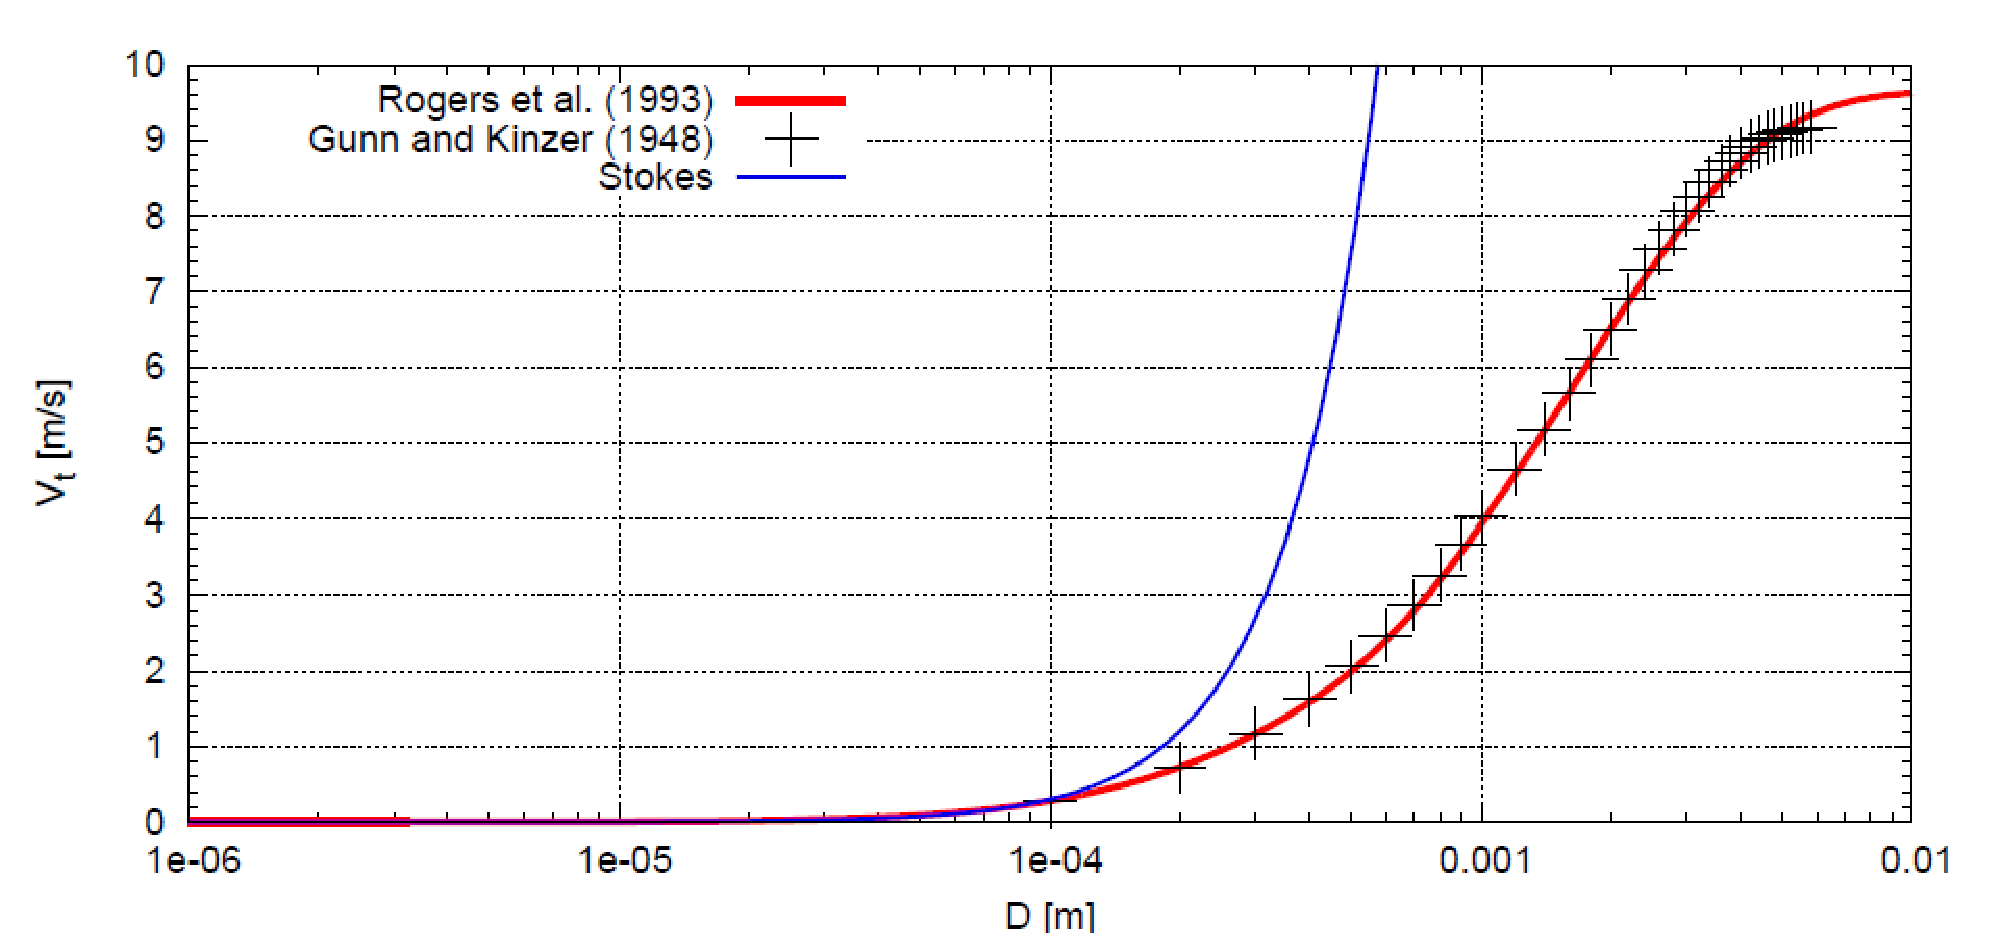
\includegraphics[scale=0.3]{./figure/D_vt_sn14.eps}
\end{center}
\caption{Dependency of terminal velocity of liquid water droplet on diameter. Marks are from Gunn and Kinzer (1948), red line is from Rogers et al. (1993) and blue line is calculated by Stokes’ law (eq.\ref{sn12}) under the condition T=293K, p=1000hPa.}
\label{figsn2-11}
\end{figure}

\begin{figure}[htbp]
\begin{center}
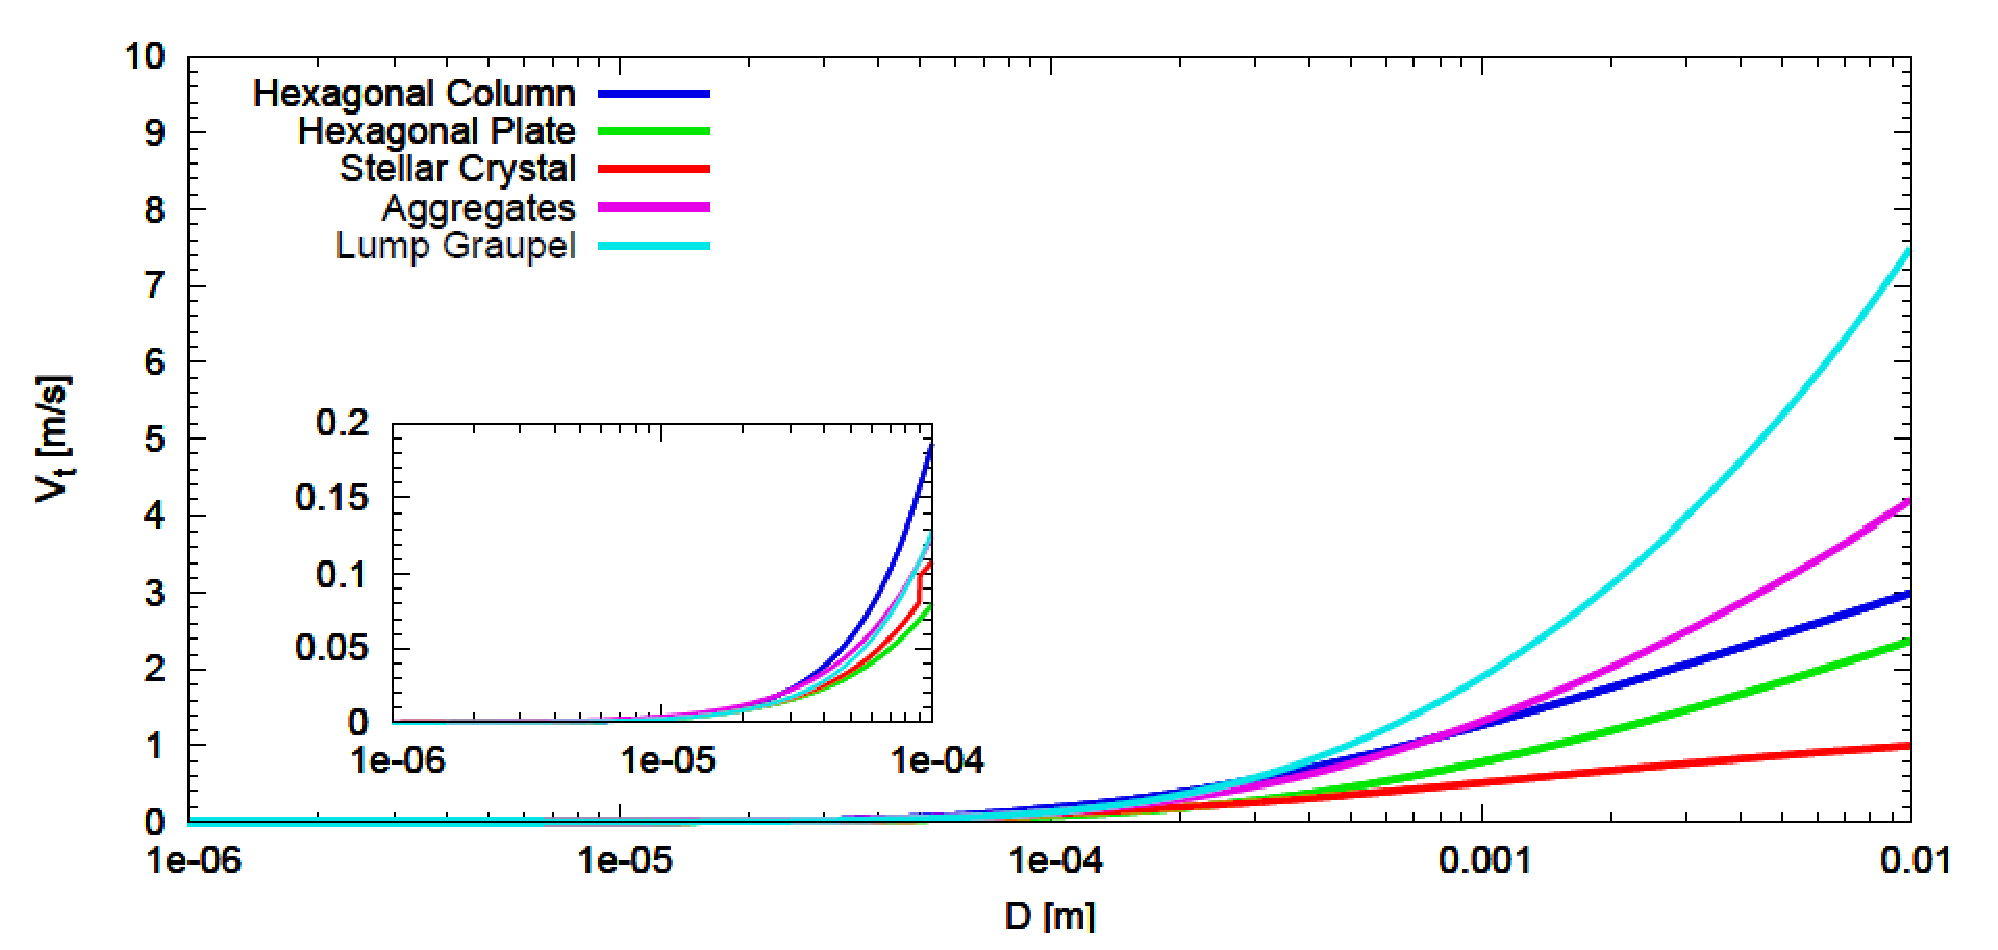
\includegraphics[scale=0.3]{./figure/D_vt_sn14-ice.eps}
\end{center}
\caption{Dependency of terminal velocity of liquid water droplet in maximum dimension. Each color of solid line is corresponding to different ice particle type based on Mitchell (1996). Hexagonal columns is blue, hexagonal plates is green, stellar crystal with broad arms is red, Aggregates of planar polycrystals in cirrus clouds is purple and lump graupel is light blue.}
\label{figsn2-12}
\end{figure}

\begin{figure}[htbp]
\begin{center}
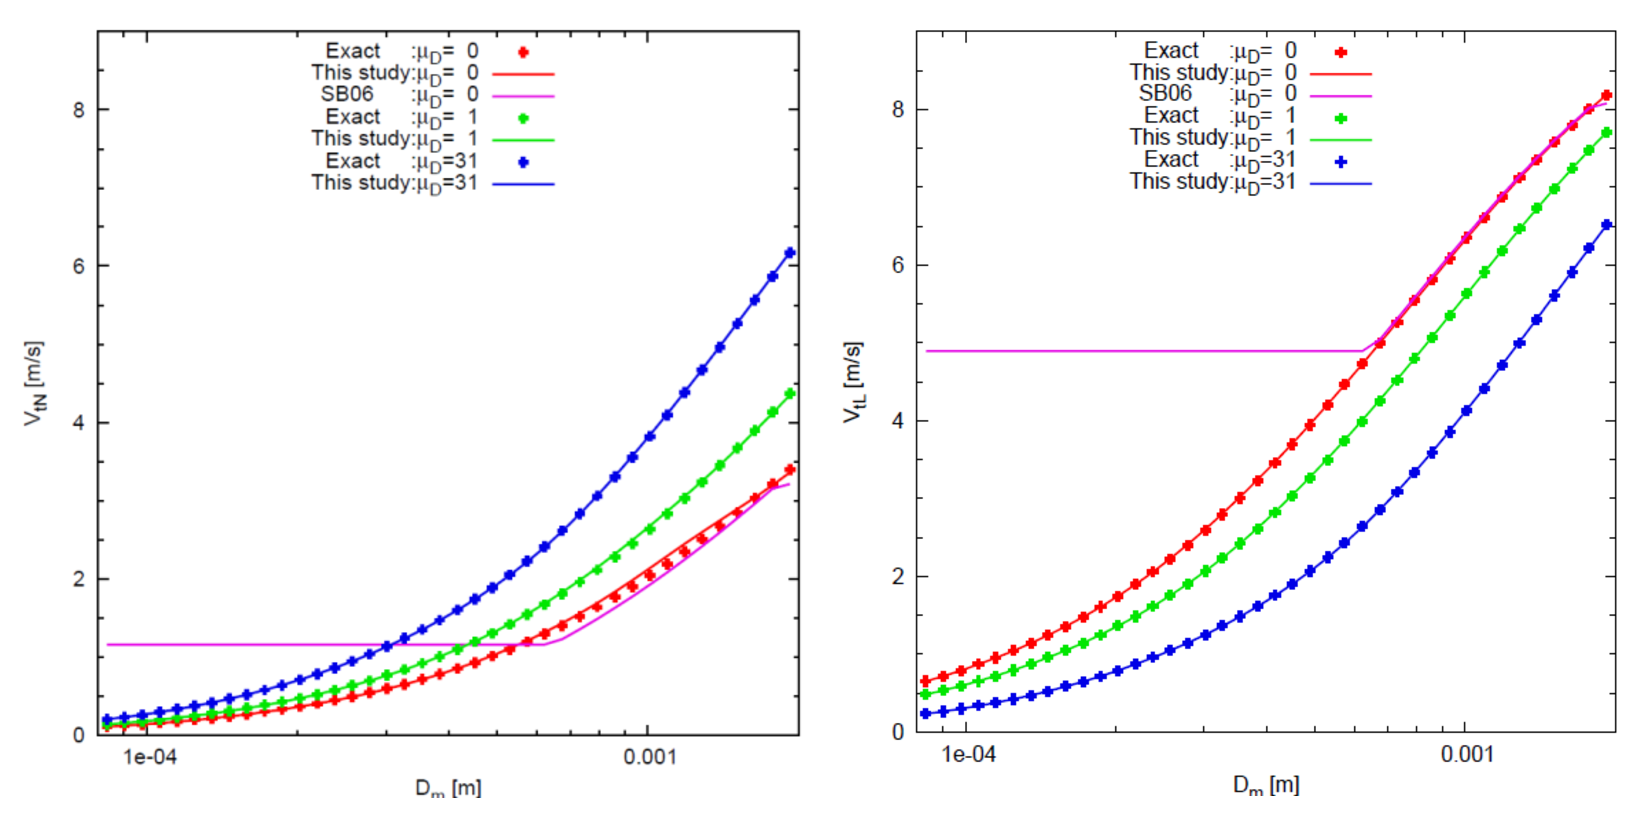
\includegraphics[scale=0.4]{./figure/D_vt_sn14-1.eps}
\end{center}
\caption{Dependencies of number weighted terminal velocity ($v_{tN}$) (left) and mass weighted terminal velocity ($v_{tL}$) (right) of rain droplets on mean volume diameter ($D_{m}$). Abscissa is the mean volume diameter and vertical axis is the terminal velocity. Dots show exactly integrated value and solid lines show approximated value by this study (red, green and blue) and Seifert and Beheng (2006) (purple). Red and purple ones are calculated with $\mu D$ = 0, green ones are calculated with $\mu D$ = 1 and blue ones are calculated with $\mu D$ = 31.}
\label{figsn2-13}
\end{figure}

\begin{figure}[htbp]
\begin{center}
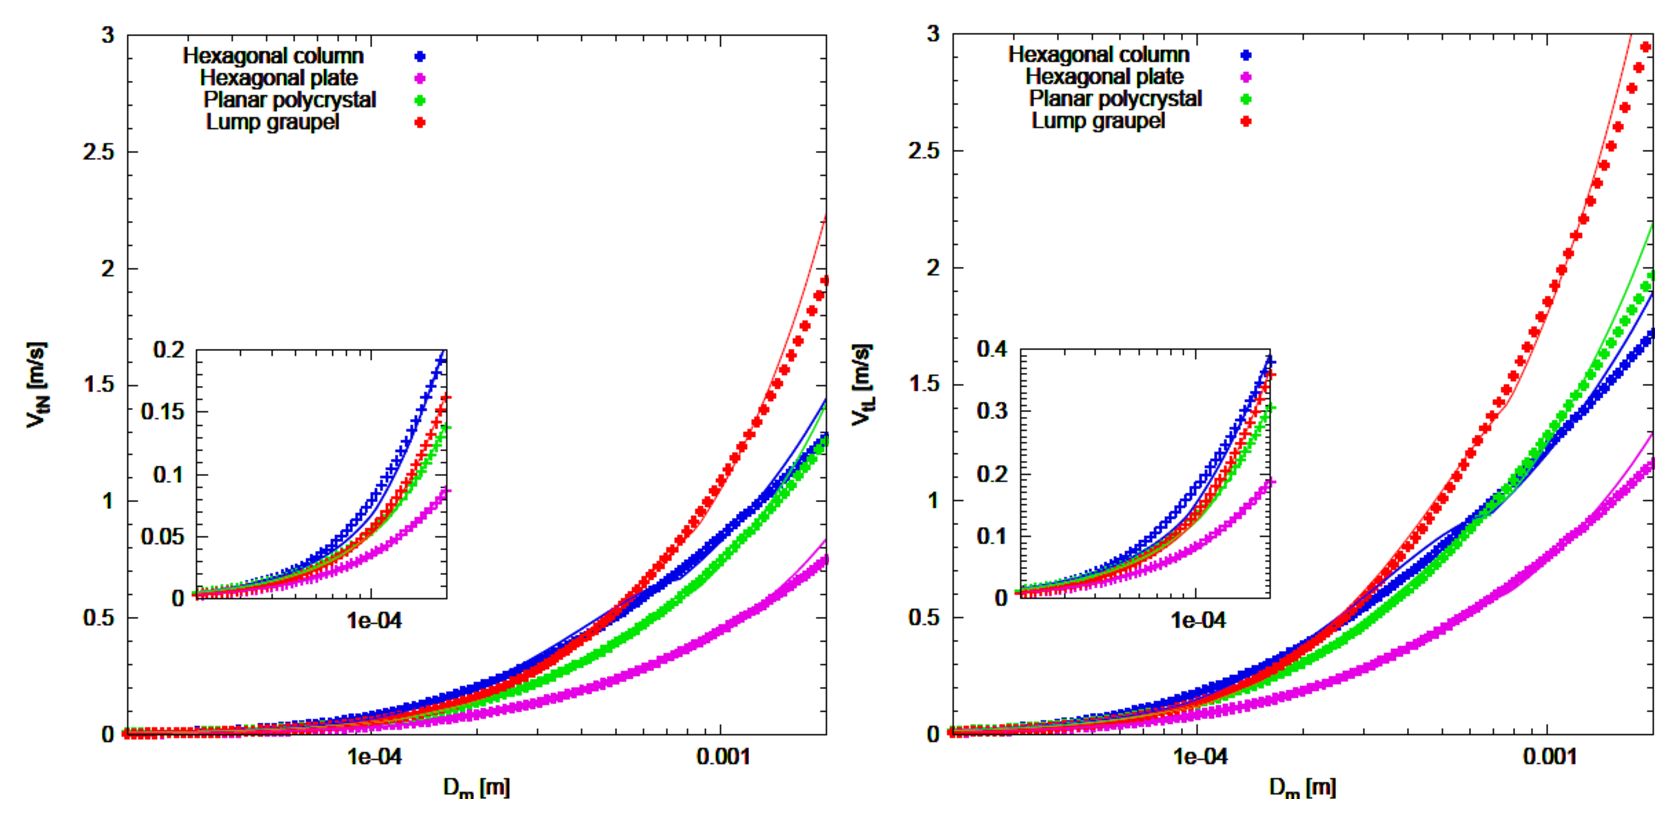
\includegraphics[scale=0.4]{./figure/D_vt_sn14-ice-1.eps}
\end{center}
\caption{Dependencies of number weighted terminal velocity ($v_{tN}$) (left) and mass weighted terminal velocity ($v_{tL}$) (right) of ice particles on mean volume diameter ($D_{m}$). Abscissa is the mean volume diameter and vertical axis is the terminal velocity. Dots show the exact value calculated by Mitchell (1996) and solid lines show the fitting curves. Red, green, blue and purple denote lump graupels, assemblages of planar polycrystals, hexagonal columns and hexagonal plates respectively.}
\label{figsn2-14}
\end{figure}

\subsubsection{Detailed description of cloud microphysics}
Cloud microphysics is mainly categorized into two physics. One is phase change among the gas, liquid, and solid phases. Another is the collection process among all the particles. In addition, all the hydrometeors are vertically transported by gravitational sedimentation. Phase change depends on the thermodynamics of environment air and affects thermodynamics itself through latent heat release. In contrast, collection is an internal growth process with less interaction with the atmosphere. Since the growth speed of the collection process is much faster than that of phase change, the role of the collection process is a key to determine the lifetime of cloud (e.g. lifetime effect). Finally, gravitational sedimentation determines the removal rate of cloud from the atmosphere. Directly it removes cloud by transportation, and indirectly by the collection process via collision volume (swept volume).\\
The cloud microphysics scheme developed in this study basically follows Seifert and Beheng (2006). Their two-moment bulk cloud microphysics scheme is remarkable in improvement of the collection process by using a bin cloud microphysics scheme. After their works, we modify the cloud nucleation process (Twomey 1959; and Lohmann 2002), the condensation process (Morrison et al. 2005), and the formulation of the terminal velocities (Mitchell, 1996) with expectation of the application to global cloud resolving simulations. We describe production and reduction terms of the mass concentration and the number concentration in the following sub-sections.

\subsubsection{Phase change}
\subsubsection{Condensation/evaporation}
Theoretical formulation of condensation or evaporation is basically derived by balance equation of vapor and thermal diffusion above the surface of a single particle (Rogers and Yau, 1989; Pruppacher and Klett, 1997). The growth rate of liquid droplet mass $x_{i}$l is described as follows,

\begin{eqnarray}
\frac{dx_{jl}}{d}&=&2\pi D(x_{jl})G_{lv}(T,p)F_{vf}(x_(jl))S_{w},\; (jl=c,r)\label{sn66}\\
G_{lv}&=&\Bigl[\frac{R_{v}T}{p_{sw}(T)D_{v}}+\frac{L_{v0}}{K_{T}T}\bigl(\frac{L_{v0}}{R_{v}}{T}-1\bigr)\Bigr]^{-1}\label{sn67}\\
F_{vf}(x_{r})&=&a_{vf,r}+b_{vf,r}N_{S_{c}}^{1/3}N_{R_{e}}^{1/2}\label{sn68}
\end{eqnarray}

Here $G_{lv}$ is a coefficient related with vapor and thermal diffusion, $D_{v}$ is diffusivity of water vapor and $K_{T}$ is thermal conductivity, and $F_{vf}$ is the so-called ventilation coefficient. This is a correction factor for assumption that the water vapor field surrounding each droplet is spherically symmetrical. Formulation of Fvf was experimentally determined by Pruppacher and Klett (1997) and it depends on Schmidt number ($N_{S_{c}}$) and Reynolds number ($N_{R_{e}}$). This formulation for single droplets is transformed into that for moments following to Seifert and Beheng (2006). With assumption of DSD as a generalized Gamma distribution and neglecting the change of DSD caused by other process in a time step, we can derive the growth rate of moments,

\begin{eqnarray}
\frac{\partial M_{jl}^{k}}{\partial t}\Bigr|_{cnd,evp}\cong \int_{0}^{\infty}f_{jl}(x)x^{k-1}\frac{\partial x}{\partial t}\Bigr|_{cnd,evp}dx\label{sn69}
\end{eqnarray}

we can consider eq.\ref{sn69} from a different view point as follows,

\begin{eqnarray}
\frac{\partial M_{jl}^{k}}{\partial t}\Bigr|_{cnd,evp}&\cong& \int_{0}^{\infty}f_{jl}(x)x^{k}\Bigl[\frac{1}{x}\frac{\partial x}{\partial t}\Bigr|_{cnd,evp}\Bigr]dx\nonumber\\
&=&\int_{0}^{\infty}\frac{f_{jl}(x)x^{k}}{\tau}dx,\;\tau\equiv\frac{x}{\frac{\partial x}{\partial t}}\bigr|_{cnd,evp}\label{sn70}
\end{eqnarray}

Here, we mention that the theoretical treatment of condensation or evaporation change droplet mass only. Then, we diagnose the growth rates of other moments by the change ratio of droplet mass with time scale $\tau$. Thus, we can derive the growth equation for arbitrary moments,

\begin{eqnarray}
\frac{\partial M_{jl}^{k}}{\partial t}\Bigr|_{cnd,evp}&=&2\pi G_{lv}S_{w}\int_{0}^{\infty}D_{jl}(x)F_{vf,jl}(x)f_{jl}(x)x^{k-1}dx\nonumber\\
&=&2\pi G_{lv}S_{w}N_{jl}D_{jl}(\bar{x}_{jl})\bar{F}_{vf,k,jl}(\bar{x}_{jl})\bar{x}_{jl}^{k-1}\label{sn71}
\end{eqnarray}

where $\bar{F}_{vf,k,il}$ is an averaged ventilation factor for the k-th moment of DSD. This formulation seems to be valid unless reduction of number concentration occurs. Because reduction of number concentration occurs only in the case of the smallest droplet being completely dissipated by evaporation, the formulation by change ratio is not suitable for complete dissipation. Therefore this formulation is incomplete to derive the reduction tendency of number concentration by evaporation (condensation never changes number concentration). Temporarily, we assumed that the number concentration of cloud droplets never reduces unless their mean mass of cloud ($\bar{x}_{c}$) falls below the lower limit $\bar{x}_{c,min}$. The treatment of rain droplets is discussed in the following section.


\subsubsection{Evaporation of rain droplets}
Only in the case of rain droplets, Seifert (2008) attempted to overcome the incompleteness for the reduction of number concentration in evaporation. He reformulated eq.\ref{sn71} as follows,

\begin{eqnarray}
\frac{\partial N_{r}}{\partial t}\Bigr|_{evp}\equiv \gamma_{evp}\frac{N_{r}}{L_{r}}\frac{\partial L_{r}}{\partial t}=\frac{\gamma_{evp}}{\bar{x}}2\pi G_{lv}S_{w}N_{r}D_{r}(\bar{x}_{r})\bar{F}_{vf,l}(\bar{x}_{r})\label{sn72}
\end{eqnarray}

Here evaporation parameter $\gamma_{evp}$ means the evaporation efficiency of number concentration towards to mean mass $\bar{x}_{r}$. According to Seifert (2008), $\gamma_{evp}$ and $\mu_{m,r}$ are parameterized as follows,

\begin{eqnarray}
\gamma_{evp}&=&\frac{D_{eq}}{D(\bar{x}_{r})}exp(-0.2\mu_{m,r})\label{sn73}\\
\mu_{m,r}&=&
\left\{
\begin{array}{l}
6tauh[{c_{evp,1}(D(\bar{x}_{r})-D_{eq})}^{2}]+1\;\;(D(\bar{x}_{r})\leq D_{eq}) \\
30tauh[{c_{evp,2}(D(\bar{x}_{r})-D_{eq})}^{2}]+1\;\;(D(\bar{x}_{r})\leq D_{eq})
\label{sn74}
\end{array}
\right.
\end{eqnarray}

where $D_{eq} = 1.1 \times 10^{-3} m$ is the equilibrium diameter in breakup-coalescence processes and the $c_{evp,1}$ and $c_{evp,2}$ are set to 4000 $m^{-1}$ and 1000 $m^{-1}$, respectively. In this study, we apply eq.\ref{sn71} for mass and eq.\ref{sn72} with $\gamma_{evp}$ = 1 for number concentration as a default setting (refer to SB06-run).

\subsubsection{Deposition/sublimation for solid water}
Theoretical formulation of deposition or sublimation is the same as that of condensation or evaporation except for the definition of surface area. The shape of ice particles is not spherical and varies widely as is shown in section 2.1.2. Therefore, vapor and thermal transfer over the particle surface is expressed by the analogy between the diffusion equation and equations in electrostatics (Pruppacher and Klett, 1997). Replacing diameter $D_{js}$ by capacitance $C_{js}\equiv D{js}/c_{js}$, we can derive the growth equation of a single particle as follows,

\begin{eqnarray}
\frac{dx_{js}}{dt}\Bigr|_{dep,sbl}&=&4\pi C_{js}G_{sv}(T,p)F_{vf}(x_{js})S_{i},\;\;(js=i,s,g)\label{sn75}\\
G_{sv}&=&\Bigl[\frac{R_{v}T}{p_{si}(T)D_{v}}+\frac{L_{s,0}}{K_{T}T}\bigl(\frac{L_{s0}}{R_{v}T}-1\bigr)\Bigr]^{-1}\label{sn76}
\end{eqnarray}

Here $C_{js}$ = $D_{js}/2$ for sphere, $C_{js} = D_{js}/\pi$ for circular plate, and capacitances of other typical shapes such as oblate spheroid crystals and columnar crystals are expressed by,

\begin{eqnarray}
C_{js}&=&\frac{D_{js}\varepsilon}{2sin^{-1}\varepsilon},\;\;\varepsilon\equiv\bigl(1-\frac{b^{2}}{a^{2}}\bigr), \;(for\;spheroid)\label{sn77}\\
C_{js}&=&\frac{A}{ln[(a+A)/b]},\;A\equiv=(a^{2}-b^{2})^{1/2},\;\;(for\;columnar)
\end{eqnarray}

where a is semi-major axis and b is semi-minor axis. For simplification, cloud, rain, snow and graupel are assumed as sphere and hexagonal plate ice is assumed as circular plate here. In the same manner as condensation (evaporation), we can derive the growth equation of arbitrary moments as follows,

\begin{eqnarray}
\frac{\partial M_{js}^{k}}{\partial t}\Bigr|_{dep,sbl}=\frac{4\pi}{c_{js}}G_{sv}S_{i}N_{js}D_{js}(\bar{x}_{js})\bar{F}_{vf,k}(\bar{x}_{js})\bar{x}_{js}^{k-1}\label{sn79}
\end{eqnarray}

Discussion concerning the reduction term of number concentration is the same as that for rain droplets. Therefore, we applied eq.\ref{sn79} for mass concentration of solid particles. For snow and graupel, the reduction rate of number concentration is as follows,

\begin{eqnarray}
\frac{\partial N_{js}^{k}}{\partial t}\Bigr|_{sbl}&\equiv&\frac{N_{js}}{L_{js}}\frac{\partial L_{js}}{\partial t}\Bigr|_{sbl}\nonumber\\
&=&\frac{1}{\bar{x}_{js}}\frac{4\pi}{c_{js}}G_{sv}S_{i}N_{js}D_{js}(\bar{x}_{js})\bar{F}_{vf,1}(\bar{x}_{js})(js=s,g)\label{sn80}
\end{eqnarray}

This formulation corresponds to $\gamma_{evp} = 1$ in the reduction term for rain droplets. That means sublimation occurs so as not to change the mean mass of DSD ($\bar{x}_{js}$). Number concentration of ice never reduces in sublimation unless the mean mass of ice ($\bar{x}_{i}$) falls below the lower limit. The formulations of the reduction rate for the number concentration of ice particles are somewhat temporary and will be improved by the insights drawn from the results of microphysics bin schemes and observations in future work.

\subsubsection{Accurate integration method to solve condensation/evaporation and deposition/sublimation}
The condensation/evaporation process for cloud droplets usually requires a smaller time step than rain droplets or other particles because of its timescale. When we apply the time integration with the first ordered Euler method, the accuracy of the condensation/evaporation and the deposition/sublimation processes are worse unless we resolve their timescale. We estimate the timescale with the exact thermodynamic definition in NICAM initially and then formulate an accurate method to apply the condensation process and the evaporation process for cloud droplets similar to Khvorostyanov and Sassen (1998) and Morrison et al., (2005). Since the supersaturated condition is achieved by updraft of air mass, we consider a Lagrangian parcel model with constant updraft velocity and no mixing with external air mass. Basic formulation is based on the Lagrangian change rate of supersaturation ($\delta_{sw} = q_{v} - q_{sw}$) as follows,

\begin{eqnarray}
\frac{d \delta_{sw}}{dt}=\Bigl(\frac{dq_{v}}{dt}-\frac{dq_{sw}}{dt}\Bigr)\label{sn81}
\end{eqnarray}

Hereafter we consider the tendency of specific humidity and saturation specific humidity by dynamics, cloud microphysics and radiative heating.\\
At first, assuming an adiabatically ascending/descending parcel with no phase change ($q_{v}/dt = 0$), eq.(\ref{sn81}) becomes

\begin{eqnarray}
\frac{d\delta_{sw}}{dt}=-\bigl(\frac{\partial q_{sw}}{\partial T}\bigr)_{p}\frac{dT}{dt}-\bigl(\frac{\partial q_{sw}}{\partial p}\bigr)_{T}\frac{dp}{dt}\label{sn82}
\end{eqnarray}

Here the tendencies of temperature and pressure are described as follows,

\begin{eqnarray}
\frac{dT}{dt}=\frac{1}{\rho\bar{c}_{p}}\frac{dp}{dt},\;\;\frac{dp}{dt}\approx-\rho g w\label{sn83}
\end{eqnarray}

where $\bar{c}_{p}\equiv q_{d}c_{pd}+q_{v}c_{pv}+q_{liq}c_{l}+q_{sol}c_{i}$ is the mean specific heat at constant pressure. We can derive the dynamic component of the tendency of $\delta_{sw}$ by substituting eq. \ref{sn83} into eq.\ref{sn82} as follows

\begin{eqnarray}
\frac{d\delta_{sw}}{dt}\Bigr|_{DYN}=wg\Bigl(\frac{1}{\bar{c}_{p}}\bigl(\frac{\partial q_{sw}}{\partial T}\bigr)_{p}+\rho\bigl(\frac{\partial q_{sw}}{\partial p}\bigr)_{T}\Bigr)\label{sn84}
\end{eqnarray}

Assuming air parcel with only cooling/heating by latent heat release, eq. \ref{sn81} becomes

\begin{eqnarray}
\frac{d\delta_{sw}}{dt}=\frac{dq_{v}}{dt}-\bigl(\frac{\partial q_{sw}}{\partial T}\bigr)\frac{dT}{dt}\label{sn85}
\end{eqnarray}

The tendency of temperature is caused by latent heat release with condensation/evaporation and deposition/sublimation %eq.\ref{sn58}; eq.\ref{sn59} %; and Table \ref{table_sn14-2-11}

\begin{eqnarray}
\frac{dT}{dt}&=&\frac{L_{v,00}+(c_{vv}-c_{l})T}{\bar{c}_{va}}\frac{dq_{liq}}{dt}+\frac{L_{v,00}+L_{f,00}+(c_{v}-c_{i})T}{\bar{c}_{va}}\frac{dq_{sol}}{dt}\nonumber\\
&=&\frac{L_{v,00}+(c_{vv}-c_{l}) T}{\bar{c}_{va}} \sum^{jl_{max}}_{jl=1}\frac{dq_{jl}}{dt}\Bigr|_{cnd,evp}\nonumber\\
&+&\frac{L_{v,00}+L_{f,00}+(c_{vv}-c_{i})T}{\bar{c}_{va}}\sum^{js_{max}}_{js=1}\frac{dq_{js}}{dt}\Bigr|_{dep,sbl}\label{sn86}
\end{eqnarray}

The tendency of specific humidity is caused by condensation/evaporation and deposition/sublimation,

\begin{eqnarray}
\frac{dq_{v}}{dt}=-\sum_{jl=1}^{jl_{max}}\frac{dq_{jl}}{dt}\Bigl|_{cnd,evp}-\sum_{js=1}^{js_{max}}\frac{dq_{js}}{dt}\Bigr|_{dep,sbl}\label{sn87}
\end{eqnarray}

Then, we can derive the cloud microphysics component of the tendency of $\delta_{sw}$ by substituting eq.\ref{sn86} and eq.\ref{sn87} into eq.\ref{sn85},

\begin{eqnarray}
\frac{d\delta_{sw}}{dt}\Bigr|_{MP}&=&-\Bigl(1+\frac{L_{v,00}+(c_{vv}-c_{l})T}{\bar{c}_{v}}\bigl(\frac{\partial q_{sw}}{\partial T}\bigr)_{p}\Bigr)\sum_{jl=1}^{jl_{max}}\partial{dq_{jl}}{dt}\Bigr|_{cnd,evp}\nonumber\\
&-&\Bigl(1+\frac{L_{v,00}+L_{f,00}+(c_{vv}-c_{i})T}{\bar{c}_{v}}\bigl(\frac{\partial q_{sw}}{\partial T}\bigr)_{p}\Bigr)\sum^{js_{max}}_{js=1}\frac{dq_{js}}{dt}\Bigr|_{dep,sbl}\label{sn88}
\end{eqnarray}

By replacing the source term of the mixing ratio of hydrometeors in eq.\ref{sn88} with eq.\ref{sn71} and eq.\ref{sn79}

\begin{eqnarray}
\frac{dq_{jl}}{dt}\Bigr|_{cnd,evp}&=&\frac{\delta_{sw}}{\tau_{cnd,jl}},\;or\nonumber\\
\frac{dq_{jl}}{dt}\Bigr|_{cnd,evp}&=&\frac{\delta_{si}}{\tau_{cnd,jl}}-\frac{q_{sw}-q_{si}}{\tau_{cnd,jl}},\;\;(jl=c,r)\label{89}\\
\frac{dq_{js}}{dt}\Bigr|_{de,sbl}&=&\frac{\delta_{si}}{\tau_{dep,js}},\;or\nonumber\\
\frac{dq_{js}}{dt}\Bigr|_{dep,sbl}&=&\frac{\delta_{sw}}{\tau_{dep,js}}+\frac{q_{sw}-q_{si}}{\tau_{dep,js}},\;\;(js=i,s,g)\label{90}\\
\tau_{cnd,jl} &\equiv& \Bigl(\frac{1}{\rho q_{sw}} 2\pi G_{lv}D_{jl}(\bar{x}_{jl})N_{jl}\bar{F}_{vf,1}\Bigr)^{-1}\label{sn91}\\
\tau_{dep,js} &\equiv& \Bigl(\frac{1}{\rho q_{si}}\frac{4\pi}{c_{js}}G_{sv}D_{js}(\bar{x}_{js})N_{js}\bar{F}_{vf,1}\Bigr)^{-1}\label{sn92}
\end{eqnarray}


We can rewrite eq.\ref{sn88} as a function of super saturation itself,
\begin{eqnarray}
\frac{\partial \delta_{sw}}{\partial t}\Bigr|_{MP}=&-&\bigl(\frac{a_{liq,liq}}{\tau_{cnd,c}}+\frac{a_{liq,liq}}{\tau_{cnd,r}}+\frac{a_{sol,liq}}{\tau_{dep}}+\frac{a_{sol,liq}}{\tau_{dep,s}}+\frac{a_{sol,liq}}{\tau_{dep,g}}\bigr)\delta_{sw}\nonumber\\
&-&\bigl(\frac{1}{\tau_{dep,i}}+\frac{1}{\tau_{dep,s}}+\frac{1}{\tau_{dep,g}}\bigr)(q_{sw}-q_{si})\label{sn93}\\
a_{liq,liq}&\equiv& 1+\frac{L_{v00}+(c_{vv}-c_{l})T}{\bar{c}_{v}}\bigl(\frac{\partial q_{sw}}{\partial T}\bigr)_{p}\label{94}\\
a_{sol,liq}&\equiv& 1+\frac{L_{v00}+L_{f00}+(c_{vv}-c_{i})T}{\bar{c}_{v}}\bigl(\frac{\partial q_{sw}}{\partial T}\bigr)_{p}\label{95}
\end{eqnarray}

Here, we can find that $\tau_{cnd,jl}$ and $\tau_{dep,js}$ in eq.\ref{sn93} are considered as the characteristic time scale to relax the super saturation condition by the condensation/evaporation and deposition/sublimation processes. The timescale of each hydrometeor is modified by coefficient $a_{liq,liq}$ or$ a_{sol,liq}$, which means the effect of latent heat release. The second term on the right hand side in eq.\ref{sn93} means the transfer of vapor from liquid droplets to solid particles. The Bergeron-Findeisen process is implicitly formulated by the difference of saturation vapor pressure between liquid and solid.\\
Finally assuming an air parcel with radiative heating (cooling), eq.\ref{sn81} becomes

\begin{eqnarray}
\frac{d\delta_{sw}}{dt}\Bigr|_{RAD}=-\bigl(\frac{\partial q_{sw}}{\partial T}\bigr)_{\rho}\bigl(\frac{dT}{dt}\bigr)_{RAD}\label{sn96}
\end{eqnarray}

All the components in the Lagrangian ascending/descending parcel model are described by eq.\ref{sn84}, eq.\ref{sn93} and eq.\ref{sn96},

\begin{eqnarray}
\frac{d\delta_{sw}}{dt}&=&A_{cnd}-\frac{\delta_{sw}}{\tau_{cnd}}\label{sn97}\\
A_{cnd}&\equiv&\frac{d\delta_{sw}}{dt}\Bigr|_{DYN}+\frac{d\delta_{sw}}{dt}\Bigr|_{RAD}\nonumber\\
&-&\bigl(\frac{1}{\tau_{dep,i}}+\frac{1}{\tau_{dep,s}}+\frac{1}{\tau_{dep,g}}\bigr)(q_{sw}-q_{si})\label{sn98}\\
\tau_{cnd}&\equiv&\bigl(\frac{a_{liq,liq}}{\tau_{cnd,c}}+\frac{a_{liq,liq}}{\tau_{cnd,r}}+\frac{a_{sol,liq}}{\tau_{dep,i}}+\frac{a_{sol,liq}}{\tau_{dep,s}}+\frac{a_{sol,liq}}{\tau_{dep,g}}\bigr)^{-1}\label{sn99}
\end{eqnarray}

Here, we can see that $A_{cnd}$ is a production term of super saturation and τcnd is a characteristic timescale of all the phase changes. From their formulation (eq.\ref{sn91} and eq.\ref{sn92}), we can find that the timescale of each hydrometeor is in inverse proportion to its number concentration. The timescales under various conditions are shown in Fig.\ref{figsn2-19}.\\
Assuming that time variance of the production term and the timescale in a simulation time step don’t vary much within a model timestep, we can analytically solve eq.\ref{sn97},

\begin{eqnarray}
\delta_{sw}(t)=A_{cnd}\tau_{cnd}+(\delta_{sw}(t_{0})-A_{cnd}\tau_{cnd})exp\bigl(-\frac{t}{\tau_{cnd}}\bigr)\label{sn100}
\end{eqnarray}

where $t = t_{0} + \Delta t$ and $t_{0} = 0$. Then, the condensation (evaporation) rate of cloud and rain are reformulated by substituting eq.\ref{sn100} into eq.\ref{sn71} and integrating them,

\begin{eqnarray}
\frac{\Delta L_{jl}}{\Delta t}\Bigr|_{cnd,evp}&=&\rho A_{cnd}\frac{\tau_{cnd}}{\tau_{cnd,jl}}\nonumber\\
&-&\rho\frac{(\delta_{sw}(t_{0})-A_{cnd}\tau_{cnd})}{\Delta t}\frac{\tau_{cnd}}{\tau_{cnd,jl}}\Bigl[exp\bigl(-\frac{\Delta t}{\tau_{cnd}}\bigr)-1\Bigr]\label{sn101}
\end{eqnarray}

This semi-analytical formulation takes time variability of super saturation into condensation (evaporation) growth. Therefore, it is better than direct time integration with a first order Euler method.\\
In the same manner, we can also derive the semi-analytical formulation for deposition (sublimation) with super saturation for solid water ($\delta_{si}$),

\begin{eqnarray}
\delta_{si}(t)&=&A_{dep}\tau_{dep}+(\delta_{si}(t_{0})-A_{dep}\tau_{dep})exp\bigl(-\frac{t}{\tau_{dep}}\bigr)\label{sn103}\\
\frac{\Delta L_{js}}{\Delta t}\Bigr|_{dep,sbl}&=&\rho A_{dep}\frac{\tau_{dep}}{\tau_{dep,js}}\nonumber\\
&-&\rho\frac{(\delta_{si}(t_{0})-A_{dep}\tau_{dep})}{\Delta t}\frac{\tau_{dep}}{\tau_{dep,js}}\Bigl[exp\bigl(-\frac{\Delta t}{\tau_{dep}}\bigr)-1\Bigr]\label{sn104}
\end{eqnarray}

where

\begin{eqnarray}
A_{dep}&\equiv&\frac{d\delta_{si}}{dt}\Bigr|_{DYN}+\frac{d\delta_{si}}{dt}\Bigr|_{RAD}\nonumber\\
&+&\bigl(\frac{1}{\tau_{cnd,c}}+\frac{1}{\tau_{cnd,r}}\bigr)(q_{sw}-q_{si})\label{sn105}\\
\tau_{dep}&\equiv&\bigl(\frac{a_{liq,sol}}{\tau_{cnd,c}}+\frac{a_{liq,sol}}{\tau_{cnd,r}}+\frac{a_{sol,sol}}{\tau_{dep,i}}+\frac{a_{sol,sol}}{\tau_{dep,s}}+\frac{a_{sol,sol}}{\tau_{dep,g}}\bigr)^{-1}\label{sn106}\\
a_{liq,sol}&\equiv&1+\frac{L_{v00}+(c_{vv}-c_{l})T}{\bar{c}_{v}}\bigl(\frac{\partial q_{si}}{\partial T}\bigr)_{p}\nonumber\\
a_{sol,sol}&\equiv&1+\frac{L_{v00}+L_{f00}+(c_{vv}-c_{i})T}{\bar{c}_{v}}\bigl(\frac{\partial q_{si}}{\partial T}\bigr)_{p}\nonumber\\
\frac{d\delta_{si}}{dt}\Bigr|_{DYN}&=&wg\Bigl(\frac{1}{\bar{c}_{p}}\bigl(\frac{\partial q_{si}}{\partial T}\bigr)_{p}+\rho\bigl(\frac{\partial q_{si}}{\partial p}\bigr)_{T}\Bigr)\nonumber\\
\frac{d\delta_{si}}{dt}\Bigl|_{RAD}&=&-\bigl(\frac{\partial q_{si}}{\partial T}\bigr)_{\rho}\bigl(\frac{dT}{dt}\bigr)_{RAD}\nonumber
\end{eqnarray}

Finally we applied eq.\ref{sn101} and eq.\ref{sn104} for the prediction of mass concentration and eq.\ref{sn72} and eq.\ref{sn80} for the prediction of number concentrations of rain, snow and graupel. Number concentrations of cloud and ice are assumed not to change by evaporation and sublimation.


\subsubsection{Nucleation of cloud droplets}
Seifert and Beheng (2006) applied traditional empirical formulation as an aerosol activation spectrum as follows,

\begin{eqnarray}
N_{c}(S_{w,100})=C_{ccn}S_{w,100}^{\kappa_{ccn}}\label{sn107}
\end{eqnarray}

where super saturation ratio $S_{w,100}$ is in %. They use $C_{ccn} = 1.26 \times 10^{9} m^{-3}$ and $\kappa_{ccn} = 0.308$ in continental conditions and $C_{ccn} = 1.0 \times 10^{8} m^{-3}$ and $\kappa_{ccn} = 0.462$ in maritime conditions. Further, Seifert and Beheng (2006) transformed eq.\ref{sn107} into a tendency formulation by time differentiation of the activation spectrum,

\begin{eqnarray}
\frac{\partial N_{c}}{\partial t}&=&
\left\{
\begin{array}{l}
C_{ccn}\kappa_{ccn}S_{w,100}^{\kappa_{ccn}-1}\frac{\partial S_{w,100}}{\partial z}w\nonumber\\
(S_{w,100}>0,\;w\frac{\partial S_{w,100}}{\partial z}>0,\;and\;S_{w,100}<1.1) \nonumber\\
0,\;\;(else)
\end{array}
\right.\\
\label{sn108}
\frac{\partial L_{c}}{\partial t}\Bigr|_{nuc}&=&x_{c,nuc}\frac{\partial N_{c}}{\partial t}\Bigr|_{nuc}\label{sn109}
\end{eqnarray}

where $x_{c,nuc} = 10^{-12} kg$ is an arbitrary mass of nucleated droplets. Because the aerosol activity spectrum is a function of supersaturation and unbounded by the total aerosol number concentration, we chose an upper limit of activated aerosols as $1.5 \times C_{ccn}$, as similarly chosen by SB06: The maximum acticated aerosol number concentration is 1.5 times of the activated aerosol number concentration at ssw = 1 $^{o}/_{o}$. Here, we should mention that this formulation depends on the grid value of super saturation ratio, vertical velocity and vertical derivation of the super saturation ratio. Since super saturation significantly varies in tens of meters above cloud base (see Fig.\ref{figsn2-21}), accurate prediction of super saturation and its vertical derivation is quite difficult. In this study, we applied a traditional nucleation scheme (Twomey, 1959; Rogers and Yau, 1989) following Morrison et al. (2005),

\begin{eqnarray}
N_{c,nuc}(w_{eff})&=&0.88C_{ccn}^{2/(\kappa_{ccn}+2)}(0.07w_{eff}^{3/2})^{\kappa_{ccn}/(\kappa_{ccn}+2)}\label{sn110}\\
w_{eff}&\equiv&w+w_{TB}-\frac{\bar{c}_{p}}{g}\bigl(\frac{dT}{dt}\bigr)_{RAD}\label{sn111}
\end{eqnarray}

where $w_{eff}$ is effective vertical velocity for nucleation and $w_{TB}$ is the sub-grid variability of terminal velocity. This is an analytical formulation of maximum number concentration around the cloud base for the Twomey equation with aerosol activated spectrum by eq.\ref{sn107} (see Fig.\ref{figsn2-18}). By using this scheme we do not have to resolve the vertical variability of super saturation around the cloud base. Furthermore, applying sub-grid turbulence effects on vertical velocity reduces under estimation of nucleated cloud number concentration caused by low horizontal resolution (Ghan, et al., 1997; Lohmann, 2002; Morrison and Pinto, 2005). In this study, implementation of the sub-grid turbulence effect follows Lohmann (2002),

\begin{eqnarray}
w_{TB}&=&c_{TB}\bigl(\frac{2}{3}TKE\bigr)^{1/2}\label{sn112}\\
\bar{N}_{c,nucl}&=&0.1\times N_{c,nuc}(w_{eff})^{1.27}\label{sn113}
\end{eqnarray}

where $c_{TB} = 1$ is used in this study, $\bar{N}_{c,nuc}$ $cm^{-3}$ is a grid averaged nucleated cloud number concentration and $N_{c,nuc}(w_{eff}) cm^{-3}$ is maximum cloud number concentration in turbulent air. By substituting eq.\ref{sn110}, eq.\ref{sn111} and eq.\ref{sn112} into eq.\ref{sn113}, the tendency of cloud number concentration is calculated by,

\begin{eqnarray}
\frac{\partial N_{c}}{\partial t}\Bigr|_{nucl}&=&
\left\{
\begin{array}{l}
\frac{N_{c,nu}(w_{eff})-N_{c}}{\Delta t},\;\;(S_{w}>0,\;\bar{N}_{c,nuc}>N_{c}\;and\;at\;cloud\;base) \\
0,\;\;(else) \\
\label{sn114}
\end{array}
\right.\\
\frac{\partial L_{c}}{\partial t}\Bigr|_{nuc}&=&min\Bigl(x_{c,min}\frac{\partial N_{c}}{\partial t}\bigr|_{nuc},\frac{\delta_{sw}}{\Delta t}\Bigr)\label{sn115}
\end{eqnarray}

Since nucleation is usually limited around the cloud base within several tens of meters (see Fig.\ref{figsn2-21}), we define cloud base layer ($k_{cbase}$) where the nucleation scheme works as follows,

\begin{eqnarray}
1.5 \times C_{ccn} > \bar{N}_{c,nu}(k_{cbase})>0,\;\;and\;\;\bar{N}_{c,nu}(k_{cbase}-1) < 10^{6}\label{sn116}
\end{eqnarray}

In addition, we prepare the option (NO-TB) to switch off the effect of turbulence by substituting eq.\ref{sn110}, eq.\ref{sn111} with $w_{TB} = 0$ into eq.\ref{sn114}. There remain some problems to be solved in future,\\
1.Definition of cloud base is empirical and arbitrary\\
2.Implementation of sub-grid scale is empirical and $c_{TB}$ is a kind of tuning parameter. In particular, the TKE approach only considers isotropic eddies. Sub-grid should be expressed as sub-grid cloud dynamics.\\
3.Formulation of eq.\ref{sn113} does not converge with the NO-TB option when TKE = 0.\\
We need to investigate the above problems by using a large eddy simulation (LES) cloud model.

\subsubsection{Nucleation of cloud ice}
This study employed two simple ice nucleation schemes, which don’t require the properties of ice nuclei. One is the depositional and condensational freezing nucleation scheme parameterized by Meyers et al. (1992),

\begin{eqnarray}
N_{IN}=10^{3}exp(-0.639+12.96S_{sol})\nonumber
\end{eqnarray}

where $N_{IN}$ is nucleated ice nuclei, and $S_{sol}$ is supersaturation for solid water. While this scheme is widely used in CRMs (e.g., Walko et al. 1995; Khain et al., 2000; Seifert and Beheng, 2006), this scheme could not be acceptable for conditions at temperature below -20 degC or supersaturation over 0.25 where observational data were not available in their study. For simulating cirrus clouds around the tropopause, application of this scheme to CRMs may cause significant error. Phillips et al. (2007) proposed an alternative scheme to modify Meyers’s scheme by fitting to observational data at temperature between -30 degC and -80 degC taken by Demott et al. (2003),

\begin{eqnarray}
N_{IN}=10^{3}exp[0.3\times12.96(S_{i}-0.1)]\label{sn117}
\end{eqnarray}

In this study, the nucleation rate is formulated by the newly nucleated ice nuclei with the tendency of supersaturation in the same manner as Murakami (1990),

\begin{eqnarray}
\frac{\Delta N_{i}}{\Delta t}&=&
\left\{
\begin{array}{l}
\frac{\partial N_{IN}}{\partial S_{sol}}\frac{\partial S_{sol}}{\partial t},\;\;(S_{sol}>0\;and\;\frac{\partial S_{sol}}{\partial t}>0) \\
0,\;\;(else) \\
\end{array}
\right.\\
\label{sn118}
\frac{\partial S_{sol}}{\partial t}&\approx& \Bigl[\frac{\partial S_{sol}}{\partial z}w+\bigl(\frac{\partial S_{sol}}{\partial T}\bigr)\bigl(\frac{\partial T}{\partial t}\bigr)_{RAD}\Bigr]\nonumber\\
\frac{\Delta L_{i}}{\Delta t}\Bigr|_{nuc}&=&\frac{\Delta N_{i}}{\Delta t}\Bigr|_{nuc}x_{IN}\label{sn119}
\end{eqnarray}

where $x_{IN} = 10^{-12} kg$ is an arbitrary parameter for a nucleated ice nuclei mass. Here, we assume the change of supersaturation comes from the vertical motion of airmass and the radiative cooling. Meyers’s scheme produces the number concentration of cloud ice more than Phillips’s scheme, and the departure becomes large as supersaturation increases. This difference would come from the sampled air masses used in observational data that their schemes referred to, and also implicit dependencies of their schemes on temperature and aerosol species. It is expected that Phillips’s scheme is appropriate for the simulation of mid-latitude cirrus clouds because Phillips’s scheme is based on the air mass sampled in the free troposphere at the mid-latitude while Meyers’s scheme is based on the air mass sampled in the atmospheric boundary layer where ice nuclei is rich.

\subsubsection{Freezing}
The freezing process consists of two types of mechanisms. One is the homogenous freezing which is freezing of supercooled water droplets for themselves without the other agents. Another is the heterogeneous freezing, which is freezing of supercooled water droplets with insoluble part of aerosols dissolved in cloud droplets. We apply the same parameterizations of both the homogeneous freezing and the heterogeneous freezing as Seifert and Beheng (2006a). Cotton and Field (2002) parameterized homogeneous freezing rate for a single droplet by a fitting to the theoretical estimation by Jeffery and Austin (1997). We apply their parameterization as Seifert and Beheng (2006a),

\begin{eqnarray}
\frac{1}{f_{c}(x)}\frac{\partial f_{c}(x)}{\partial t}\Bigr|_{hom}=-xJ_{hom}(T_{c})\label{sn120}
\end{eqnarray}

where $J_{hom}$ is a homogeneous freezing rate ($kg^{-1}s^{-1}$) and $T_{c}$ is centigrade temperature. $J_{hom}$ is formulated as a function of temperature as follows,

\begin{eqnarray}
log_{10}(10^{-3}J_{hom})=
\left\{
\begin{array}{l}
25.63-243.4-14.75T_{c}-0.307T_{c}^{2},\;\;(-65^{o}C>T_{c}) \nonumber \\
-0.00287T_{c}^{3}-0.0000102T_{c}^{4},\;\;(-65^{o}C\leq T_{c}<-30^{o}C)\nonumber \\
-7.63-2.996(T_{c}+30),\;\;(-30^{o}C< T_{c})\nonumber
\end{array}
\label{sn121}
\right.
\end{eqnarray}

Based on the equation for a single droplet, we can derive the equation for moments by integrating eq.\ref{sn120} as follows

\begin{eqnarray}
\frac{\partial N_{c}}{\partial t}\Bigr|_{hom}&=&-L_{c}J_{hom}=-N_{c}\bar{x}_{c}J_{hom}\label{sn122}\\
\frac{\partial L_{c}}{\partial t}\Bigr|_{hom}&=&-Z_{c}J_{hom}=-\frac{\Gamma\bigl(\frac{\nu_{c}+3}{\mu_{c}}\bigr)\Gamma\bigl(\frac{\nu_{c}+1}{\mu_{c}}\bigr)}{\Gamma\bigl(\frac{\nu_{c}+2}{\mu_{c}}\bigr)^{2}}L_{c}\bar{x}_{c}J_{hom}\label{sn123}
\end{eqnarray}

Here, we mention that eq.\ref{sn122} and eq.\ref{sn123} are expressed via filtered $\bar{x}_{c}$ in order to avoid artificial value of the prognostic variables. The homogeneous freezing for rain is not considered because it is negligible compared with the heterogeneous freezing due to their largeness. Although Cotton and Field (2002) considered also freezing point depression in freezing due to soluble aerosols, we don’t consider the effect because Seiki and Nakajima (2014) is not yet coupled with aerosol transport models.
Heterogeneous freezing is based on the empirical formulation by Biggs (1953) which is widely used in CRMs.

\begin{eqnarray}
\frac{1}{f(x)}\frac{\partial f(x)}{\partial t}=-xJ_{het}(T_{c})\label{sn124}
\end{eqnarray}

where $J_{het}$ is the heterogeneous freezing rate. $J_{het}$ is formulated as a function of temperature as follows,

\begin{eqnarray}
J_{het}=A_{het}exp(-B_{het}T_{c}-1)\label{sn125}
\end{eqnarray}

whare $A_{het}=0.2kg^{-1}s^{-1}$ and $B_{het}=0.65K^{-1}$ are empirically determined parameters. Similar to the homogeneous freezing, we can derive the equation for moments as follows,

\begin{eqnarray}
\frac{\partial N_{il}}{\partial t}\Bigr|_{het}&=&-N_{il}\bar{x}_{il}J_{het}\;\;(il=c,r)\label(sn126)\\
\frac{\partial L_{il}}{\partial t}\Bigr|_{het}&=&-\frac{\Gamma\bigl(\frac{\nu_{il}+3}{\mu_{il}}\bigr)\Gamma\bigl(\frac{\nu_{il}+1}{\mu_{il}}\bigr)}{\Gamma\bigl(\frac{\nu_{il}L2}{\mu_{il}}\bigr)^{2}}L_{il}\bar{x}_{il}J_{het}\;\;(il=c,r)\label{sn127}
\end{eqnarray}

Although the heterogeneous freezing should be also formulated as a function of aerosol concentration, here we apply simple formulation because our model is not yet coupled with an aerosol transport model.\\
Thus, these parameterizations don’t include the information of aerosols and it is considered that they assume background aerosols. The validity of the parameterization was demonstrated by Khain et al. (2001). Nevertheless their model also applied the same simple freezing parameterizations, they could represented the observational features of supercooled liquid water by Rosenfeld and Woodley (2000). Both freezing rates are shown in Fig. \ref{figsn2-22}. The heterogeneous freezing is dominated at temperature over -35 degrees Celsius. At the temperature, supercooled liquid water is mixed with ice particles. In contrast, the homogeneous freezing rate suddenly increase below -35 degrees Celsius. Liquid water droplets have been hardly observed below the temperature of -40 degrees Celsius (Rosenfeld and Woodley, 2000). The feature can be represented by using the parameterization.

\subsubsection{Melting}
Melting process is the same as Seifert and Beheng (2006a) based on Pruppacher and Klett (1997). Theoretical treatment of this process is similar to the condensation process. The differences are\\
1.Time scale of evaporation of a single particle is replaced by that of fusion of a single particle.\\
2.Vaporization of melted particle is considered in a balance equation of vapor and thermal diffusion.\\
As a result, the melting rate of a single ice particle is described as follows,

\begin{eqnarray}
\frac{dx_{js}}{dt}\Bigr|_{mlt}=&-&\frac{2\pi D_{js}}{L_{f0}}\Bigl[K_{T}(T-T_{0})\frac{D_{T}}{D_{v}}F_{vf}(x_{js})\nonumber\\
&+&\frac{D_{v}L_{v0}}{R_{v}}\bigr(\frac{p_{v}}{T}-\frac{p_{sw}(T_{0})}{T}\bigr)F_{vf}(x_{js})\Bigr]\;\;(js=i,s,g)\label{sn128}
\end{eqnarray}

where $D_{T}$ is diffusivity of heat, and $T_{0} = 273.15 K$ is melting point. The growth rate of moments can be formulated by using a melting time scale $\tau_{mlt}$ defined as follows,

\begin{eqnarray}
\tau_{mlt}&\equiv&\frac{x_{js}}{\bigl(\frac{dx_{js}}{dt}\bigr)_{mlt}}\label{sn129}\\
\frac{\partial M_{js}^{k}}{\partial t}\Bigr|_{mlt}&=&-\int_{0}^{\infty}\frac{x^{k}f_{js}(x)}{\tau_{mlt}}dx\nonumber\\
&=&-\frac{2\pi}{L_{f0}}\Bigl[\frac{K_{T}D_{T}}{D_{v}}(T-T_{0})+\frac{D_{v}L_{v0}}{R_{v}}\bigl(\frac{p_{v}}{T}-\frac{p_{sw}(T_{0})}{T_{0}}\bigr)\Bigr]\nonumber\\
&\times& N_{js}D_{js}(\bar{x}_{js})x_{js}^{n-1}\bar{F}_{vf,js}
\label{sn140}
\end{eqnarray}

We mention that this scheme allows the existence of ice particles over the melting point ($T>273.15 K$) since the melting time scale of large particles can be longer than a simulation time step. Actually, ice particles are transitionally converted into liquid droplets and the type of hydrometeor is not changed in the transition. However, here we assume that ice water mass is converted into liquid water mass in a certain melting time scale and the part of liquid water mass is categorized as the other hydrometeors. Here, graupel and snow is converted into rain, and ice is converted into cloud. This formulation has a possibility to cause an artificial production of cloud or rain in melting. Validation experiments and impact assessment are necessary in future.

\subsubsection{Collection process}
The collection processes are the same as Seifert and Beheng (2001), Seifert and Beheng (2006a) and Seifert (2008). The collection processes among hydrometeors are summarized in Table \ref{table_sn14-16}. In this section, the formulations of the collection processes, auto-conversion, accretion, aggregation, riming, and their related processes are described.


\begin{table}[h]
\begin{center}
\caption{Hydrometeors that result from binary collision. Collecting hydrometeors are written in the 1st row and collected hydrometeors are written in the 1st column.}
\label{table_sn14-16}
\scalebox{0.5}{
\begin{tabular}{cccccc}
\hline
             &  cloud water & rain & cloud ice & snow & graupel  \\ \hline
cloud water  &  rain        & -    & -         & -    & -        \\ \hline
rain         &  rain        & rain & rain($T>273K$), graupel($T<273K$) & rain($T>273K$), graupel($T<273K$) & rain($T>273K$) \\ \hline
cloud ice    &  cloud ice   & -    & snow      & -    & - \\ \hline
snow         &  snow        & -    & -     & snow & - \\ \hline
graupel      &  graupel     & graupel($T<273K$) & graupel & graupel & - \\ \hline
\end{tabular}
}
\end{center}
\end{table}

\subsubsection{Self-collection, auto-conversion, and accretion}
With a few assumptions and a little algebra, Seifert and Beheng (2001) derived the analytical formulations of the self-collection, auto-conversion, and accretion processes as follows,

\begin{eqnarray}
\frac{\partial N_{c}}{\partial t}\Bigr|_{aut+sle}&=&-k_{cc}\frac{(\nu_{c}+2)}{(\nu_{c}+1)}\frac{\rho_{0}}{\rho}L_{c}^{2}\label{sn142}\\
\frac{\partial L_{c}}{\partial t}\Bigr|_{aut}&=&-\frac{k_{cc}}{20x^{*}}\frac{(\nu_{c}+2)(\nu_{c}+4)}{(\nu_{c}+1)^{2}}\frac{\rho_{0}}{\rho}L_{c}^{2}x_{c}^{2}\label{sn143}\\
\frac{\partial N_{c}}{\partial t}\Bigr|_{aut}&=&\frac{2}{x^{*}}\frac{\partial L_{c}}{\partial t}\Bigr|_{aut}\label{sn144}\\
\frac{\partial N_{r}}{\partial t}\Bigr|_{aut}&=&-\frac{1}{2}\frac{\partial N_{c}}{\partial t}\Bigr|_{aut}=-\frac{1}{x^{*}}\frac{\partial L_{c}}{\partial t}\Bigr|_{aut}\label{sn145}\\
\frac{\partial N_{c}}{\partial t}\Bigr|_{acc}&=&-k_{cr}N_{c}L_{r}\bigl(\frac{\rho_{0}}{\rho}\bigr)^{1/2}\label{sn146}\\
\frac{\partial L_{c}}{\partial t}\Bigr|_{acc}&=&-k_{cr}L_{c}L_{r}\bigl(\frac{\rho_{0}}{\rho}\bigr)^{1/2}\label{sn147}\\
\frac{\partial N_{r}}{\partial t}\Bigr|_{slc}&=&-k_{rr}L_{r}L_{r}\bigl(\frac{\rho_{0}}{\rho}\bigr)^{1/2}\label{sn148}
\end{eqnarray}
with $k_{rr} = 4.33 m^{3}kg^{-1}s^{-1}$, and where density factors are introduced by Seifert and Beheng (2006a) in order to correct the effect of terminal velocity on the collision efficiency. In addition to the analytical derivation, Seifert and Beheng (2001) made corrections depending on the development stage by using the dimensionless internal time scale. Since moment bulk methods cannot represented complicated changes of high-order moments, the corrections are necessary as DSD undergoes evolution by the collection processes. Firstly, the auto-conversion rate is represented by $\tau$ by substituting eq.\ref{sn141} to eq.\ref{sn143},
\begin{eqnarray}
\frac{\partial \tau}{\partial t}\Bigr|_{aut}=\frac{k_{cc}}{20x^{*}}\frac{(\nu_{c}+2)(\nu_{c}+4)}{(\nu_{c}+1)^{2}}\frac{\rho_{0}}{\rho}x_{c}^{2}L(1-\tau^{2})\label{sn149}
\end{eqnarray}

The assumptions used in the derivation of eq.\ref{sn149} are valid for the initial stage of collisional growth. Therefore, the additional collection by a universal function $\phi_{aut}$ was introduced by Seifert and Beheng (2001) as follows,
\begin{eqnarray}
\frac{\partial \tau}{\partial t}\Bigr|_{aut}=\frac{k_{cc}}{20x^{*}}\frac{(\nu_{c}+2)(\nu_{c}+4)}{(\nu_{c}+1)^{2}}\frac{\rho_{0}}{\rho}x_{c}^{2}L_{c}^{2}x_{c}^{2}\bigl[(1-\tau^{2})+\phi_{aut}(\tau)\bigr]\label{sn150}
\end{eqnarray}

Similarly, the correction for the accretion rate is also made by a universal function $\phi_{acc}$,
\begin{eqnarray}
\frac{\partial \tau}{\partial t}\Bigr|_{acc}=k_{cr}L\bigl(\frac{\rho_{0}}{\rho}\bigr)^{1/2}(1-\tau)\tau\phi_{acc}(\tau)\label{sn151}
\end{eqnarray}

In contrast to the correction for the auto-conversion rate, the assumptions used in the derivation of the accretion rate is valid for the mature stage of the collisional growth. Therefore a correction function is multiplied so that $\phi_{aut}$ becomes zero for the beginning of the collisional growth and one for the mature stage of the collisional growth. Here, it is recognized that the growth rate of the dimensional internal time scale is proportional to LWC in eq.\ref{sn150} and eq.\ref{sn151}. Therefore, the parameterizations developed by Seifert and Beheng (2001) satisfy the similarity included in the SCE. Finally, the universal functions are derived by fitting to the results by a bin cloud microphysics model,
\begin{eqnarray}
\phi_{aut}(\tau)&=&400\tau^{0.7}(1-\tau^{0.7})^{3}\label{152}\\
\phi_{acc}(\tau)&=&\bigl(\frac{\tau}{\tau+5\times 10^{-5}}\bigr)^{4}\label{153}
\end{eqnarray}

These functions are shown in Fig.\ref{figsn2-21}.\\
Here, we mention that the fitting curves of the universal functions highly depend on the calculation by a bin cloud microphysics model. In fact, the functions proposed by Seifert and Beheng (2006a) were modified from the original functions by Seifert and Beheng (2001) with the progresses in the estimation of the collection kernel. We have to update the parameterizations when more sophisticated collection kernel will be estimated than the one used by Seifert and Beheng (2006a)

\subsubsection{Break-up}
Large rain droplets are not always stable in the collision process. It was observed that large rain droplets could break up into many small droplets after the collision ( Low and Lists, 1982 ). Collisional break-up sustain mean droplet size so as not to grow extremely larger and cause strong precipitation. As discussed by Hu and Srivastava (1995), the system of collision, coalescence and break-up reaches the equilibrium condition between coalescence and break-up after the sufficient long time. Consequently the form of the DSD of rain is led to the self-similar equilibrium DSD with the equilibrium mean diameter $\bar{D}_{eq}$ . Seifert and Beheng (2006a) simply parameterized the break-up process as a relaxation of the DSD with the mean diameter more than $\bar{D}_{eq}$ to the self-similar equilibrium DSD.

\begin{eqnarray}
\frac{\partial N_{r}}{\partial t}\Bigr|_{brk}=-\bigl[\phi_{brk}(\Delta \bar{D}_{r})+1\bigr]\frac{\partial N_{r}}{\partial t}\Bigr|_{slc}\label{sn154}
\end{eqnarray}

where $\phi_{brk}$ is a universal function of break-up, and $\Delta \bar{D}_{r}\equiv \bar{D}_{r}-\bar{D}_{eq}$, $\bar{D}_{r}$ is the mean volume diameter of rain, with $\bar{D}_{eq} = 1.1 mm$ according to Seifert (2008). The universal function was derived by a fitting to the results by a bin cloud microphysics model based on ( Seifert et al. 2005 ), and formulated as follows,

\begin{eqnarray}
\phi_{brk}(\Delta\bar{D}_{r})=
\left\{
\begin{array}{l}
2exp(\kappa_{brk}\Delta\bar{D}_{r})-1,\;\;(\bar{D}_{r}>\bar{D}_{eq}) \\
\kappa_{brk}\Delta\bar{D}_{r}+1,\;\;(\bar{D}_{eq}\geq \bar{D}_{r}>0.35\times 10^{-3}m) \\
-1,\;\;(0.35\times10^{-3}>\bar{D}_{r})
\label{sn155}
\end{array}
\right.
\end{eqnarray}

with $\kappa_{brk} = 2.3 \times 10^{3} m^{-1}$, and $k_{brk} = 1000 m^{-1}$. For the mean volume diameter less than $0.35 \times 10^{-3}m$, break-up is neglected.

\subsubsection{Mixed-phase collection}
In the previous sections, the collection processes are limited for warm cloud. In this section, the collection processes among mixed phase clouds are described. In contrast to warm cloud, there exist many kinds of particles in cold cloud as discussed in section 2.1. Since the variety of the shape and their coexistence condition differs case by case, there are no systematized theory, observation, and experiments for the mixed phase collection processes. Therefore, Seifert and Beheng (2006a) proposed a general formulation of the collisional interactions among hydrometeors starting from the simplification of the SCE. Due to the variety of the types of hydrometeors, the patterns of the interaction are categorized into following five cases.\\
1.A particle of hydrometeor “a” collects “b” and then the collecting particle “a” grow. This pattern is corresponding to the collision between ice and cloud (ic), snow and cloud (sc), graupel and cloud (gc), snow and ice (si), graupel and rain (gr), and graupel and snow (gs).\\
2.A particle of hydrometeor “a” collects “b” and then the other particle “c” is produced. This pattern is corresponding to the collision between rain and ice (ri), and rain and snow (rs).\\
3.A particle of hydrometeor “a” collects “a” and then the other particle “b” is produced. This pattern is corresponding to the collision between ice and ice (ii).\\
4.A particle of hydrometeor “a” collects “a” and then the collecting particle “a” grows. This pattern is corresponding to the collision between snow and snow (ss).\\
In the following sections, we introduce the derivation of the mixed phase collection corresponding to the five cases.

\subsubsection{The collision case 1: a+b $\rightarrow$ a}
In contrast to the SCE for warm cloud, the production term and reduction term are slightly different in the binary collision between two types of hydrometeors. The reduction term of the hydrometeor “b” and the production term of the hydrometeor “a” are described as follows,

\begin{eqnarray}
\frac{\partial f_{b}(y)}{\partial t}\Bigr|_{col,ab}&=&-\int_{0}^{\infty}f_{b}(y)f_{a}(x)K_{ab}(x,y)dx\label{sn156}\\
\frac{\partial f_{b}(y)}{\partial t}\Bigr|_{col.ab}&=&\int_{0}^{\infty}f_{a}(x-y)f_{b}(x)K_{ab}(x-y,y)dx\nonumber\\
&-&\int_{0}^{\infty}f_{a}(x)f_{b}(y)K_{ab}(x,y)dy\label{sn157}
\end{eqnarray}

Here, the formulation of the collection kernel is often described by the swept volume of large particle as follows,

\begin{eqnarray}
K_{ab}(x,y)\equiv E_{ab}(x,y)\frac{\pi}{4}\bigl[D_{a}(x)+D_{b}(y)\bigr]^{2}\bigl[v_{t,a}(x)-v_{t,b}(y)\bigr]\label{sn158}
\end{eqnarray}

where $E_{ab}$ is the collection efficiency, $D_{i}$ and $v_{t,i}$ are diameter and terminal velocity respectively. We can derive the growth rate of the kth moments by integrating eq.\ref{sn156} and eq.\ref{sn157},

\begin{eqnarray}
\frac{\partial M_{b}^{k}}{\partial t}\Bigr|_{col,ab}&=&\frac{\pi}{4}\int_{0}^{\infty}\int_{0}^{\infty}f_{b}(y)f_{a}(x)\bigl[D_{a}(x)+D_{b}(y)\bigr]^{2}\nonumber\\
&\times&\bigl|v_{t,a}(x)-v_{t,b}(y)\bigr|E_{ab}(x,y)y^{k}dxdy\label{sn159}\\
\frac{\partial M_{a}^{k}}{\partial t}\Bigr|_{col,ab}&=&\frac{\pi}{4}\int_{0}^{\infty}\int_{0}^{\infty}f_{a}(x)f_{b}(y)\bigl[D_{a}(x)+D_{b}(y)\bigr]^{2}\nonumber\\
&\times&\bigl|v_{t,a}(x)-v_{t,b}(y)\bigr|E_{ab}(x,y)\bigl[(x+y)^{k}-x^{k}\bigr]dxdy\label{sn160}
\end{eqnarray}

Here, the difference of the terminal velocities, and the collection efficiency in the integrand make the analytical integration of eq.\ref{sn159} and eq.\ref{sn160} impossible. In the past, many researchers have made effort to express the integration by approximation. Seifert and Beheng (2006a) achieved the integration by using the approximation proposed by Wisner et al. (1972) with some improvements. Hereafter, we only demonstrate the equations for the 0th moment N and the 1st moment L.

\begin{eqnarray}
\frac{\partial L_{b}}{\partial t}\Bigr|_{col,ab}&\cong&-\frac{\pi}{4}\bar{E}_{ab}\bar{\Delta v_{t,ab}^{1}}\nonumber\\
&\times&\int_{0}^{\infty}\int_{0}^{\infty}f_{a}(x)f_{b}(y)\bigl[D_{a}(x)+D_{b}(y)\bigr]^{2}ydxdy\label{sn161}\\
\frac{\partial L_{a}}{\partial t}\Bigr|_{col,ab}&\cong&\frac{\pi}{4}\bar{E}_{ab}\bar{\Delta v_{t,ab}^{1}}\int_{0}^{\infty}\int_{0}^{\infty}f_{a}(x)f_{b}(y)\bigl[D_{a}(x)+D_{b}(y)\bigr]^{2}ydxdy\nonumber\\
&=&-\frac{\partial L_{b}}{\partial t}\label{sn162}\\
\frac{\partial N_{b}}{\partial t}\Bigr|_{col,ab}&\cong&-\frac{\pi}{4}\bar{E}_{ab}\bar{\Delta v_{t,ab}^{0}}\int_{0}^{\infty}\nonumber\\
&\times&\int_{0}^{\infty}f_{a}(x)f_{b}(y)\bigl[D_{a}(x)+D_{b}(y)\bigr]^{2}dxdy\label{sn163}\\
\frac{\partial N_{a}}{\partial t}\Bigr|_{col,ab}&=&0\label{sn164}
\end{eqnarray}

where $\bar{E}_{ab}$ is the mean collection efficiency, and $\bar{\Delta v_{t,ab}^{k}}$ is a characteristic velocity difference. Thus, the integrand are transformed so as to be integrated analytically and the problems result in the evaluation of $\bar{E}_{ab}$ and $\bar{\Delta v_{t,ab}^{k}}$. Some cloud microphysics schemes evaluate $\bar{\Delta v_{t,ab}^{k}}$ as the approximation proposed by Wisner (1972),

\begin{eqnarray}
\bar{\Delta v_{t,ab}^{k}}=\bigl|\bar{v}_{M_{a}^{k}}(\bar{x}_{a})-\bar{v}_{M_{b}^{k}}(\bar{y}_{b})\bigr|\label{sn165}
\end{eqnarray}

The characteristic velocity difference is simply approximated by the difference between the mass weighted mean terminal velocity of the hydrometeors. This is equivalent to the physical assumption that all the particles are falling with the same terminal velocity equal to the mass weighted mean terminal velocity. However, as pointed out by Seifert and Beheng (2006a), the formulation underestimates the term for the similar mass weighted mean terminal velocities even though larger particles preferentially collect smaller particles due to their differences of the terminal velocities. Seifert and Beheng (2006a) applied an alternate approximation in order to avoid the abovementioned problem as follows,

\begin{eqnarray}
\bar{\Delta v_{t,ab}^{k}}=\Bigl[\frac{\int_{0}^{\infty}\int_{0}^{\infty}{v_{t,a}(x)-v_{t,b}(y)}^{2}D_{a}^{2}D_{b}^{2}f_{a}(x)f_{b}(y)y^{k}dxdy}
{\int_{0}^{\infty}\int_{0}^{\infty}D_{a}^{2}D_{b}^{2}f_{a}(x)f_{b}(y)y^{k}dxdy}\Bigr]^{1/2}\label{sn166}
\end{eqnarray}

The integrand can be integrated straightforwardly assuming the diameter and the terminal velocity follow power laws as given in section 2.1. Here, we apply the equivalent projected area diameter in contrast to the maximum dimension applied by Seifert and Beheng (2006a),

\begin{eqnarray}
D&=&D_{C}(x)=\bigl(\frac{4}{\pi}A\bigr)^{1/2}=a_{C}x^{b_{C}}\label{sn167}\\
a_{C}&=&\bigl(\frac{4}{\pi}a_{ax}\bigr)^{1/2},\;\;b_{C}=\frac{b_{ax}}{2}\nonumber
\end{eqnarray}

Since the diameter is used in the calculation of collisional cross section, maximum dimension overestimates collisional cross section for needle or column like crystals. Firstly, the denominator in eq.\ref{sn166} is transformed as follows,

\begin{eqnarray}
& &\int_{0}^{\infty}\int_{0}^{\infty}D_{C,a}^{2}D_{C,b}^{2}f_{a}(x)f_{b}(y)y^{k}dxdy\nonumber\\
&=&a_{C_{a}}^{2}a_{C_{b}}^{2}M_{a}^{2b_{C,a}}M_{b}^{2b_{C,b}+k}\nonumber\\
&=&D_{C,a}^{2}(\bar{x})D_{C,b}^{2}(\bar{y})\bar{y}^{k}\nonumber\\
&\times&\frac{\Gamma\bigl(\frac{2b_{C,a}+\nu_{a}+1}{\mu_{a}}\bigr)}{\Gamma\bigl(\frac{\nu_{a}+1}{\mu_{a}}\bigr)}
\frac{\Gamma\bigl(\frac{2b_{C,b}+k+\nu_{a}+1}{\mu_{a}}\bigr)}{\Gamma\bigl(\frac{\nu_{a}+1}{\mu_{a}}\bigr)}\nonumber\\
&\times&\Bigl[\frac{\Gamma\bigl(\frac{\nu_{a}+1}{\mu_{a}}\bigr)}{\Gamma\bigl(\frac{\nu_{a}+1}{\mu_{a}}\bigr)}\Bigl]^{2_{b_{C,a}}}
\Bigl[\frac{\Gamma\bigl(\frac{\nu_{b}+1}{\mu_{b}}\bigr)}{\Gamma\bigl(\frac{\nu_{b}+1}{\mu_{b}}\bigr)}\Bigl]^{2_{b_{C,b}}+k}\label{sn168}
\end{eqnarray}

Secondly, the numerator in eq.\ref{sn166} is transformed as follows,


\begin{eqnarray}
& &\int_{0}^{\infty}\int_{0}^{\infty}\bigl[v_{t,a}(x)-v_{t,b}(y)\bigr]^{2}D_{C,b}^{2}D_{C,b}^{2}f_{a}(x)f_{b}(y)y^{k}dxdy\nonumber\\
&=&a_{C_{a}}^{2}a_{C_{b}}^{2}\bigl[a_{v,a}^{2}M_{a}^{2b_{C,a}+2b_{v,a}}\nonumber\\
&+&M_{b}^{2b_{C,b}+k}-2a_{v,a}a_{v,b}M_{a}^{2b_{C,a}+b_{v,a}}M_{b}^{2b_{C,b}+b_{v,b}+k}+a_{v,b}^{2}M_{a}^{2b_{C,a}}M_{b}^{2b_{C,b}+2b_{v,b}+k}\bigr]\nonumber\\
&=&D_{C,a}^{2}(\bar{x})D_{C,b}^{2}(\bar{y})\bar{y}^{k}\nonumber\\
%\Bigl[
&+&v_{t,a}^{2}(\bar{x})
\frac{\Gamma\bigl(\frac{2b_{C,a}+2b_{v,a}+v_{a}+1}{\mu_{a}}\bigr)}{\Gamma\bigl(\frac{v_{a}+1}{\mu_{a}}\bigr)}
\frac{\Gamma\bigl(\frac{2b_{C,b}+k+v_{a}+1}{\mu_{a}}\bigr)}{\Gamma\bigl(\frac{v_{a}+1}{\mu_{a}}\bigr)}
\Bigl[\frac{\Gamma\bigl(\frac{v_{a}+1}{\mu_{a}}\bigr)}{\Gamma\bigl(\frac{v_{a}+2}{\mu_{a}}\bigr)}\Bigr]^{2_{b_{C,a}}+2b_{v,a}}
\Bigl[\frac{\Gamma\bigl(\frac{v_{b}+1}{\mu_{b}}\bigr)}{\Gamma\bigl(\frac{v_{b}+2}{\mu_{b}}\bigr)}\Bigr]^{2_{b_{C,a}}+k}\nonumber\\
&=&2v_{t,a}(\bar{x})v_{t,b}(\bar{y})
\frac{\Gamma\bigl(\frac{2b_{C,a}+b_{v,a}+v_{a}+1}{\mu_{a}}\bigr)}{\Gamma\bigl(\frac{v_{a}+1}{\mu_{a}}\bigr)}
\frac{\Gamma\bigl(\frac{2b_{C,b}+b_{v,a}+k+v_{a}+1}{\mu_{a}}\bigr)}{\Gamma\bigl(\frac{v_{a}+1}{\mu_{a}}\bigr)}\nonumber\\
&\times&\Bigl[\frac{\Gamma\bigl(\frac{v_{a}+1}{\mu_{a}}\bigr)}{\Gamma\bigl(\frac{v_{a}+2}{\mu_{a}}\bigr)}\Bigr]^{2_{b_{C,a}}+b_{v,a}}
\Bigl[\frac{\Gamma\bigl(\frac{v_{b}+1}{\mu_{b}}\bigr)}{\Gamma\bigl(\frac{v_{b}+2}{\mu_{b}}\bigr)}\Bigr]^{2_{b_{C,a}}+b_{v,b}+k}\nonumber\\
&+&v_{t,b}^{2}(\bar{y})
\frac{\Gamma\bigl(\frac{2b_{C,a}+v_{a}+1}{\mu_{a}}\bigr)}{\Gamma\bigl(\frac{v_{a}+1}{\mu_{a}}\bigr)}
\frac{\Gamma\bigl(\frac{2b_{C,b}+2b_{v,a}+k+v_{a}+1}{\mu_{a}}\bigr)}{\Gamma\bigl(\frac{v_{a}+1}{\mu_{a}}\bigr)}
\Bigl[\frac{\Gamma\bigl(\frac{v_{a}+1}{\mu_{a}}\bigr)}{\Gamma\bigl(\frac{v_{a}+2}{\mu_{a}}\bigr)}\Bigr]^{2_{b_{C,a}}}\nonumber\\
&\times&\Bigl[\frac{\Gamma\bigl(\frac{v_{b}+1}{\mu_{b}}\bigr)}{\Gamma\bigl(\frac{v_{b}+2}{\mu_{b}}\bigr)}\Bigr]^{2_{b_{C,a}}+2b_{v,b}+k}\label{sn169}
\end{eqnarray}

Finally, the characteristic velocity difference are derived by substituting eq.\ref{sn168} and eq.\ref{sn169} into \ref{sn166},

\begin{eqnarray}
\bar{\Delta v_{t,ab}^{k}}&=&\bigl[\theta_{a}^{0}v_{t,a}^{2}(\bar{x})-\theta_{ab}^{k}v_{t,a}(\bar{x})v_{t,b}(\bar{y})+\theta_{b}^{k}v_{t,b}^{2}\bigr]^{1/2}\label{sn170}\\
\theta_{a}^{k}&=&\frac{\Gamma\bigl(\frac{2b_{C,a}+2b_{v,a}+k+v_{a}+1}{\mu_{a}}\bigr)}{\Gamma\bigl(\frac{2b_{C,a}+k+v_{a}+1}{\mu_{a}}\bigr)}\Bigl[\frac{\Gamma\bigl(\frac{v_{a}+1}{\mu_{a}}\bigr)}{\Gamma\bigl(\frac{v_{b}+2}{\mu_{b}}\bigr)}\Bigr]\{2b_{v,a+k}\label{sn171}\\
\theta_{ab}^{k}&=&2\frac{\Gamma\bigl(\frac{2b_{C,a}+b_{v,a}+v_{a}+1}{\mu_{a}}\bigr)}{\Gamma\bigl(\frac{2b_{C,a}+v_{a}+1}{\mu_{a}}\bigr)}\frac{\Gamma\bigl(\frac{2b_{C,b}+b_{v,b}+k+v_{b}+1}{\mu_{b}}\bigr)}{\Gamma\bigl(\frac{2b_{C,b}+k+v_{b}+1}{\mu_{b}}\bigr)}\nonumber\\
&\times&\Bigl[\frac{\Gamma\bigl(\frac{v_{a}+1}{\mu_{a}}\bigr)}{\Gamma\bigl(\frac{v_{a}+2}{\mu_{a}}\bigr)}\Bigr]^{b_{v,a}}\Bigl[\frac{\Gamma\bigl(\frac{v_{b}+1}{\mu_{b}}\bigr)}{\Gamma\bigl(\frac{v_{b}+2}{\mu_{b}}\bigr)}\Bigr]^{b_{v,b}}\label{sn172}
\end{eqnarray}

Here, it is noticed that the notation “ab” in $\theta_{ab}^{k}$ is not symmetric because $\theta_{ab}^{k}$ is weighted by the mass of collected particle to the power of “k”. Integrations in eq.\ref{sn161} and eq.\ref{sn163} are similarly calculated as follows,


\begin{eqnarray}
& &\int_{0}^{\infty}\int_{0}^{\infty}f_{a}(x)f_{b}(y){D_{a}(x)+D_{b}(y)}^{2}y^{k}dx\nonumber\\
&=& a_{C_{a}}^{2}M_{a}^{2b_{C,a}}M_{b}^{k}+2a_{C_{a}}a_{C_{b}}M_{a}^{b_{C,a}}M_{b}^{b_{C,b}+k}+a_{C_{b}}^{2}M_{a}^{0}M_{b}^{2b_{C,b}+k}\nonumber\\
&=& \delta_{a}^{0}D_{C,a}^{2}(\bar{x})N_{a}M_{b}^{k}+\delta_{ab}^{k}D_{C,a}(\bar{x})D_{C,b}(\bar{y})N_{a}N_{b}\bar{y}^{k}\nonumber\\
&+&\delta_{b}^{k}D_{C,b}^{2}(\bar{y})N_{a}N_{b}\bar{y^{k}}\label{sn173}\\
\delta_{a}^{k}&=&\frac{\Gamma\bigl(\frac{2b_{C,b}+k+v_{a}+1}{\mu_{a}}\bigr)}{\Gamma\bigl(\frac{\mu_{a}+1}{\mu_{a}}\bigr)}\Bigl[\frac{\Gamma\bigl(\frac{v_{a}+1}{\mu_{a}}\bigr)}{\Gamma\bigl(\frac{v_{a}+2}{\mu_{a}}\bigr)}\Bigr]^{2_{b_{C,a}}+k}\label{sn174}\\
\delta_{ab}^{k}&=& 2\frac{\Gamma\bigl(\frac{b_{C,a}+v_{a}+1}{\mu_{a}}\bigr)}{\Gamma\bigl(\frac{v_{a}+1}{\mu_{a}}\bigr)}\frac{\Gamma\bigl(\frac{b_{C,b}+k+v_{b}+1}{\mu_{b}}\bigr)}{\Gamma\bigl(\frac{v_{b}+1}{\mu_{b}}\bigr)}\Bigl[\frac{\Gamma\bigl(\frac{v_{a}+1}{\mu_{a}}\bigr)}{\Gamma\bigl(\frac{v_{a}+2}{\mu_{a}}\bigr)}\Bigr]^{b_{C,a}}\Bigl[\frac{\Gamma\bigl(\frac{v_{b}+1}{\mu_{b}}\bigr)}{\Gamma\bigl(\frac{v_{b}+2}{\mu_{b}}\bigr)}\Bigr]^{b_{C,b}+k}\label{sn175}
\end{eqnarray}

Here, $\delta_{ab}^{k}$ is also asymmetry in “ab” as $\theta_{ab}^{k}$. Finally, the growth rates of the prognostic moments are represented as follows,


\begin{eqnarray}
\frac{\partial L_{a}}{\partial }\Bigr|_{col,ab}&=&\frac{\pi}{4}\bar{E}_{ab}N_{a}L_{b}{\delta_{a}^{0}D_{C,a}^{2}(\bar{x}_{a})+\delta_{ab}^{1}D_{C,a}(\bar{x}_{a})D_{C,b}(\bar{x}_{b})+\delta_{b}^{1}D_{C,b}^{2}(\bar{x}_{b})}\nonumber\\
&\times&[\theta_{a}^{0}v_{t,a}^{2}(\bar{x}_{a})-\theta_{ab}^{1}v_{t,a}(\bar{x}_{a})v_{t,b}(\bar{x}_{b})+\theta_{b}^{1}v_{t,b}^{2}(\bar{x}_{b})+\sigma_{a}+\sigma_{b}]^{1/2}\label{sn176}\\
\frac{\partial L_{b}}{\partial t}\Bigr|_{col,ab}&=&-\frac{\partial L_{a}}{\partial t}\Bigl|_{col,ab}\label{sn177}\\
\frac{\partial N_{b}}{\partial }\Bigr|_{col,ab}&=&\frac{\pi}{4}\bar{E}_{ab}N_{a}N_{b}{\delta_{a}^{0}D_{C,a}^{2}(\bar{x}_{a})+\delta_{ab}^{0}D_{C,a}(\bar{x}_{a})D_{C,b}(\bar{x}_{b})+\delta_{b}^{0}D_{C,b}^{2}(\bar{x}_{b})}\nonumber\\
&\times&[\theta_{a}^{0}v_{t,a}^{2}(\bar{x}_{a})-\theta_{ab}^{0}v_{t,a}(\bar{x}_{a})v_{t,b}(\bar{x}_{b})+\theta_{b}^{0}v_{t,b}^{2}(\bar{x}_{b})+\sigma_{a}+\sigma_{b}]^{1/2}\label{sn178}\\
\frac{\partial N_{b}}{\partial t}\Bigr|_{col,ab}&=&0\label{sn179}
\end{eqnarray}

where $\sigma_{a}$ and $\sigma_{b}$ are constant variances due to the probabilities of the terminal velocity of particles. Seifert and Beheng (2006a) proposed the concept to mimic an introduction of the effect of turbulence to the collection kernel with the use of the constant variances. The constant variances are only applied to ice and snow with $\sigma_{i}= \sigma_{s} = 0.2 m s^{-1}$ while no variances are assumed for the other particles.

\subsubsection{The collection efficiencies of ice particles}
The collection efficiencies of ice particles are poorly understood due to their varieties and the lack of the systematic observations. In addition, the efficiencies cannot be approximated by power laws. Therefore, Seifert and Beheng (2006a) described them in a simple way. The collection efficiency $E_{ab}$ can be decomposed into two part of efficiencies, the collision efficiency $E_{col}$ and the sticking efficiency $E_{stick}$. This means that two particles stochastically collide each other with $E_{col}$, and then they stick each other with $E_{stick}$. It is considered that the mean possibility of collection $\bar{E}_{ab}$ is parameterized by the multiplying $\bar{E}_{col}$ by $\bar{E}_{stick}$.

\begin{eqnarray}
\bar{E}_{ab}=\bar{E}_{col,ab}\times\bar{E}_{stick,ab}\label{sn180}
\end{eqnarray}

The mean collision efficiencies of each gydrometeor are given as follows,

\begin{eqnarray}
\bar{E}_{col,ab}&=&\bar{E}_{col,a}\times\bar{E}_{colk,b}\label{sn181}\\
\bar{E}_{col,c}&=&
\left\{
\begin{array}{l}
0,\;\;(\bar{D}_{c}<\bar{D}_{c,0}) \\
\frac{\bar{D}_{c}-\bar{D}_{c,0}}{\bar{D}_{c,1}-\bar{D}_{c,0}},\;\;(\bar{D}_{c,0}\leq\bar{D}_{c}\leq\bar{D}_{c,1}) \\
1,\;\;(\bar{D}_{c,1}<\bar{D}_{c}) \\
\end{array}
\label{sn182}
\right.\\
\bar{E}_{col,r}&=&1\label{sn183}\\
\bar{E}_{col,js}&=&
\left\{
\begin{array}{l}
0,\;\;(\bar{D}_{js}<150nm) \\
\bar{E}_{col,max,js},\;\;(\bar{D}_{js}>150nm),\;\;\;(js=i,s,g)
\label{sn184}
\end{array}
\right.
\end{eqnarray}


with $\bar{D}_{c,0} = 15\mu m$, $\bar{D}_{c,1} = 40 \mu m$, $\bar{E}_{col,max,i}=\bar{E}_{col,max,s}=0.8$ , and $\bar{E}_{col,max,g}=1.0$. Furthermore, the mean collision efficiency of one is assumed in the collision between rain droplets and ice particles, and the collision between ice particles. These values are so empirical that further investigations and assessments are required.\\
The sticking efficiency is considered only in the case of the collision between ice particles. Otherwise, the efficiency is assumed as one. It is known that the stick efficiency depends on the enviromental condition around ice particles and the shape of ice particle (Pruppacher and Klett, 1997). Ice crystals with many branches are likely to stick each other. In addition, the ice particles under wet conditions are also likely to coalescence because of the surface condition of ice particles. Since these dependencies of the stick efficiency are poorly understood, some simple formulations were proposed by past researchers. Lin et al. (1983) proposed the following formulation,

\begin{eqnarray}
\bar{E}_{stick}(T)=
\left\{
\begin{array}{l}
exp[0.09\times T_{c}],\;\;(T_{c}\leq 0^{o}C) \\
1,\;\;(T_{c}> 0^{o}C)
\label{sn185}
\end{array}
\right.
\end{eqnarray}

In contrast to their formulation, Cotton et al. (1986), proposed an alternative formulation based on observations (Hallgren and Hosler, 1960) as follows,

\begin{eqnarray}
\bar{E}_{stick}(T_{p})=min(10^{0.035(T_{p}-273.15)-0.7},0.2)\label{sn186}
\end{eqnarray}

where $T_{p}$ is particle surface temperature. They also diagnosed the departure of particle surface temperature from the enviroment due to phase change in the calculation. In addition, their formulation has a upper limit to reduce the efficiency as observations showed. In a similar way, Khain and Sednev (1996) proposed a formulation based on other observations (Hosler et al., 1957; Rogers et al., 1974). Their formulation also depends on vapor pressure as follows,

\begin{eqnarray}
\bar{E}_{stick}&=&min\bigl(\delta E\frac{p_{v}}{p_{si}},1\bigr)\label{sn187}\\
\delta E&=&max(a_{\delta}+b_{\delta}T_{c}+c_{\delta}T_{c}^{2}+d_{\delta}T_{c}^{3},0)\label{sn188}
\end{eqnarray}

with $a_{\delta} = 0.883$, $b_{\delta} = 0.093$, $c_{\delta} = 0.00348$, and $d_{\delta} = 4.5185 \times 10^{-5}$. In this study, the formulation proposed by Lin et al. (1983) is applied following Seifert and Beheng (2006a). These efficiencies are shown in Fig.\ref{figsn2-22} with the various obeservation data from Pruppacher and Klett (1997). The further investigations and assessments are necessary to determine which one is better than others although there are less information for making a decision.


\subsubsection{The collision case 2: a+b $\rightarrow$ c}
 The case is the same as the case 1 except for the growing particles.

\begin{eqnarray}
\frac{\partial f_{b}(y)}{\partial t}\Bigr|_{col,abs}&=&-\int_{0}^{\infty}f_{b}(y)f_{a}(x)K_{ab}(x,y)dx\label{sn189}\\
\frac{\partial f_{a}(x)}{\partial t}\Bigr|_{col,abs}&=&-\int_{0}^{\infty}f_{a}(x)f_{b}(y)K_{ab}(x,y)dy\label{sn190}
\end{eqnarray}

Similarly, the growth rates of the prognostic moments are derived as follows,

\begin{eqnarray}
\frac{\partial L_{a}}{\partial t}\Bigr|_{col,ab}&=&-\frac{\pi}{4}\bar{E}_{ab}\bar{\Delta v_{t,ab}^{1}}\nonumber\\
&\times& \int_{0}^{\infty}\int_{0}^{\infty}f_{a}(x)f_{b}(y)[D_{a}(x)+D_{b}(y)]^{2}xdxdy\label{sn191}\\
\frac{\partial L_{b}}{\partial t}\Bigr|_{col,ab}&=&-\frac{\pi}{4}\bar{E}_{ab}\bar{\Delta v_{t,ab}^{1}}\nonumber\\
&\times&\int_{0}^{\infty}\int_{0}^{\infty}f_{a}(x)f_{b}(y)[D_{a}(x)+D_{b}(y)]^{2}ydxdy\label{sn192}\\
\frac{\partial N_{a}}{\partial t}\bigr|_{col,ab}&=&\frac{\partial N_{b}}{\partial t}\Bigl|_{col,ab}=-\frac{\pi}{4}\bar{E}_{ab}\bar{\Delta v_{t,ab}^{0}}\nonumber\\
&\times&\int_{0}^{\infty}\int_{0}^{\infty}f_{a}(x)f_{b}(y)[D_{a}(x)+D_{b}(y)]^{2}dxdy\label{sn193}\\
\frac{\partial N_{c}}{\partial t}\bigr|_{col,ab}&=&-\frac{\partial N_{a}}{\partial t}\Bigl|_{col,ab}\label{sn194}
\end{eqnarray}

Finally, the equations are transformed by using the approximations as follows,


\begin{eqnarray}
\frac{\partial L_{b}}{\partial t}\Bigr|_{col,ab}&=&-\frac{\pi}{4}\bar{E}_{ab}{N_{a}}{L_{b}}\nonumber\\
&\times&[\delta_{a}^{0}D_{C,a}^{2}(\bar{x}_{a})+\delta_{ab}^{1}D_{C,a}(\bar{x}_{a})D_{C,b}(\bar{x}_{b})+\delta_{b}^{1}D_{C,b}^{2}(\bar{x}_{b})]\label{sn195}\\
&\times&[\theta_{a}^{0}v_{t,a}^{2}(\bar{x}_{a})-\theta_{ab}^{1}v_{t,a}(\bar{x}_{a})v_{t,b}(\bar{x}_{b})+\theta_{b}^{1}v_{t,b}^{2}(\bar{x}_{b})+\sigma_{a}+\sigma_{b}]^{1/2}\nonumber\\
\frac{\partial L_{a}}{\partial t}\Bigr|_{col,ab}&=&-\frac{\pi}{4}\bar{E}_{ab}{N_{b}}{L_{a}}\nonumber\\
&\times&[\delta_{b}^{0}D_{C,b}^{2}(\bar{x}_{b})+\delta_{ab}^{1}D_{C,a}(\bar{x}_{a})D_{C,b}(\bar{x}_{b})+\delta_{a}^{1}D_{C,a}^{2}(\bar{x}_{b})]\label{sn196}\\
&\times&[\theta_{b}^{0}v_{t,b}^{2}(\bar{x}_{b})-\theta_{ba}^{1}v_{t,a}(\bar{x}_{a})v_{t,b}(\bar{x}_{b})+\theta_{a}^{1}v_{t,a}^{2}(\bar{x}_{b})+\sigma_{a}+\sigma_{b}]^{1/2}\nonumber\\
\frac{\partial N_{b}}{\partial t}\Bigr|_{col,ab}&=&-\frac{\pi}{4}\bar{E}_{ab}{N_{a}}{N_{b}}\nonumber\\
&\times&[\delta_{a}^{0}D_{C,a}^{2}(\bar{x}_{a})+\delta_{ab}^{0}D_{C,a}(\bar{x}_{a})D_{C,b}(\bar{x}_{b})+\delta_{b}^{0}D_{C,a}^{2}(\bar{x}_{b})]\label{sn197}\\
&\times&[\theta_{a}^{0}v_{t,a}^{2}(\bar{x}_{a})-\theta_{ab}^{0}v_{t,a}(\bar{x}_{a})v_{t,b}(\bar{x}_{b})+\theta_{b}^{0}v_{t,a}^{2}(\bar{x}_{b})+\sigma_{a}+\sigma_{b}]^{1/2}\nonumber\\
\frac{\partial N_{a}}{\partial t}\Bigr|_{col,ab}&=&-\frac{\pi}{4}\bar{E}_{ab}{N_{a}}{N_{b}}\nonumber\\
&\times&[\delta_{a}^{0}D_{C,a}^{2}(\bar{x}_{a})+\delta_{ab}^{0}D_{C,b}(\bar{x}_{a})D_{C,b}(\bar{x}_{b})+\delta_{b}^{0}D_{C,b}^{2}(\bar{x}_{b})]\label{sn198}\\
&\times&[\theta_{a}^{0}v_{t,a}^{2}(\bar{x}_{a})-\theta_{ba}^{0}v_{t,b}(\bar{x}_{a})v_{t,b}(\bar{x}_{b})+\theta_{b}^{0}v_{t,b}^{2}(\bar{x}_{b})+\sigma_{a}+\sigma_{b}]^{1/2}\nonumber
\end{eqnarray}

\subsubsection{The collision case3: a+a $\rightarrow$ b}
In the case, binary collision between particles in the same hydrometeor is considered. All the pairs in the collision turn into the other hydormeteor as follows,

\begin{eqnarray}
\frac{\partial f_{a}(x)}{\partial t}\Bigr|_{col,aa}=-\int_{0}^{\infty}f_{a}(x)f_{a}(y)K_{aa}(x,y)dy\label{sn199}
\end{eqnarray}

The growth rate of the prognostic moments is as follows,

\begin{eqnarray}
\frac{\partial L_{a}}{\partial t}\Bigr|_{col,aa}&=&-\frac{\pi}{4}\bar{E}_{aa}{N_{a}}{L_{a}}\nonumber\\
&\times&{\delta_{a}^{0}D_{C,a}^{2}(\bar{x}_{a})+\delta_{aa}^{1}D_{C,a}^{2}(\bar{x}_{a})}\nonumber\\
&\times&{\theta_{a}^{0}v_{t,a}^{2}(\bar{x}_{a})-\theta_{aa}^{1}v_{t,a}^{2}(\bar{x}_{a})+2\sigma_{a}}\label{sn200}\\
\frac{\partial N_{a}}{\partial t}\Bigr|_{col,aa}&=&-\frac{\pi}{4}\bar{E}_{aa}{N_{a}}{N_{a}}\nonumber\\
&\times&{2\delta_{a}^{0}D_{C,a}^{2}(\bar{x}_{a})+\delta_{aa}^{0}D_{C,a}^{2}(\bar{x}_{a})}\nonumber\\
&\times&{2\theta_{a}^{0}v_{t,a}^{2}(\bar{x}_{a})-\theta_{aa}^{0}v_{t,a}^{2}(\bar{x}_{a})+2\sigma_{a}}\label{sn201}\\
\frac{\partial L_{b}}{\partial t}\Bigr|_{col,aa}&=&-\frac{\partial L_{a}}{\partial t}\Bigr|_{col,aa}\label{sn202}\\
\frac{\partial N_{b}}{\partial t}\Bigr|_{col,aa}&=&-\frac{1}{2}\frac{\partial N_{a}}{\partial t}\Bigr|_{col,aa}\label{sn203}
\end{eqnarray}


\subsubsection{The collision case 4: a+a $\rightarrow$ a}
In the case, self aggregational growth is considered. In the aggregation, the number concentration of the hydrometeor “a” decreases under the conservation of the mass concentration. The basic equation is the same as the case 3 except for the absence of the other hydrometeor.

\begin{eqnarray}
\frac{\partial N_{a}}{\partial t}&=&-\frac{1}{2}\frac{\pi}{4}\bar{E}_{aa}N_{a}N_{a}\nonumber\\
&\times&{2\delta_{a}^{0}D_{C,a}^{2}(\bar{x}_{a})+\delta_{aa}^{0}D_{C,a}^{2}(\bar{x}_{a})}\nonumber\\
&\times&{2\theta_{a}^{0}v_{t,a}^{2}(\bar{x}_{a})+\theta_{aa}^{0}v_{t,a}^{2}(\bar{x}_{a})+2\sigma_{a}}^{1/2}\label{sn204}
\end{eqnarray}

\subsubsection{The secondary processes}
There are several secondary processes associated with the mixed phase collection. Here, we briefly describe them following Seifert and Beheng (2006a).

\subsubsection{Enhanced melting}
We assume that the particle temperature is the same as the enviromental temperature. However, the melting process allows the existence of ice particles under the warmer condition than the melting point. In the riming process under the condition, coalescence of a liquid droplet uniformizes the temperature of colliding two particles. Subsequently, the temperature difference between a ice particle and a liquid droplet are compensated by the latent heat relase of the ice particle. In our model framework, since the category of wet ice particle is not considered, the melting part of a riming particle is accounted as the production of a liquid droplet. The melting rate by the riming process is formulated following Rutledge and Hobbs (1984),

\begin{eqnarray}
\frac{\partial L_{js}}{\partial t}\Bigr|_{eml}=-\frac{c_{1}T_{c}}{L_{f0}}\frac{\partial L_{js}}{\partial t}\Bigr|_{col}\;\;(T_{c}>0^{o}C),\;(js=i,s,g)\label{sn205}
\end{eqnarray}

Here, the reduction rate of number conentration is treated similarly to the melting process,

\begin{eqnarray}
\frac{\partial N_{js}}{\partial t}\Bigr|_{eml}=\frac{1}{\bar{x}_{js}}\frac{\partial L_{js}}{\partial t}\Bigr|_{col}\label{sn206}
\end{eqnarray}

\subsubsection{Partial convesrion}
According to Seifert and Beheng (2006a), a riming particle becomes a densely rimed spherical particle as soon as the collected liquid droplet fills up the envelop of the collecting ice particle. The produced densely rimed spherical particle is categorized as graupel. Here, we consider that the volume difference between a ice crystal or a spongy ice particle and its enveloping sphere is filled by the collected liquid droplet. The critical liquid droplet mass $\bar{x}_{crit,pcon}$ is estimated by the geometry of ice as follows,

\begin{eqnarray}
\bar{x}_{crit,pcon,js}=\alpha_{fill,js}\rho_{w}\bigl(\frac{\pi}{6}\bar{D}_{js}^{3}-\frac{\bar{x}_{js}}{\rho_{\varepsilon}},\;\;\;(js=i,s)\label{sn207}
\end{eqnarray}

where $\alpha_{fill}$ is the so-called filling coefficient, $\rho_{\varepsilon} = 900 kg m^{-3}$ is density of ice. The filling coefficient is the criterion to categorize a ice particle as graupel by its dense. Tentatively, $\alpha_{fill}$, $i = 0.68$ and $\alpha_{fill}$, $s = 0.01$ are set by Seifert and Beheng (2006a). This means that snow is categorized as almost unrimed ice particles. The characteristic conversion time scale τpcon is estimated by the growth rate of mean particle mass by the riming process as follows,

\begin{eqnarray}
\tau_{pcon,js}=\frac{\bar{x}_{crit,pcon,js}}{\frac{1}{N_{js}}\frac{\partial L_{js}}{\partial t}\Bigr|_{rime}}\label{sn208}
\end{eqnarray}

Finally, the conversion rates of riming particles into graupel are derived by using the characteristic time scale.

\begin{eqnarray}
\frac{\partial L_{g}}{\partial t}\Bigr|_{pcon}&=&\frac{L_{js}}{\tau_{pcon,js}}=min\bigl(\frac{\bar{x}_{js}}{\bar{x}_{crit,pcon,js}},1\bigr)\frac{\partial L_{js}}{\partial t}\Bigr|_{rime}\label{sn209}\\
\frac{\bar{x}_{js}}{\bar{x}_{crit,pcon,js}}&=&\Bigl[\alpha_{fill,js}\frac{\rho_{w}}{\rho_{\varepsilon}}\bigl(\frac{\pi}{6}D_{i}^{3}\rho_{i}\frac{1}{\bar{x_{js}}}-1\bigr)\Bigr]^{-1}\label{sn210}
\end{eqnarray}

The conversion rate of number concentration is as follows,

\begin{eqnarray}
\frac{\partial N_{g}}{\partial t}\Bigr|_{pcon}=\frac{1}{\bar{x}_{js}}\frac{\partial L_{g}}{\partial t}\Bigr|_{pcon}
\end{eqnarray}

The conversion coefficient of riming particle $\bar{x}/\bar{x}_{crit,pconv}$ is shown in Fig.\ref{figsn2-23}. In this formulation, small ice particles are likely to convert into graupel in riming because small ice particles have simple geometry and are almost sphere. In order to suppress the conversion of small ice particles, partial conversion are limited to ice particles with the mean diameter of more than 500 $\mu m$.

\subsubsection{Ice multiplication}
It has been observed that the number concentration of ice particles can be up to several orders of magnitude larger than ice nuclei in atmospheric cloud (Pruppacher and Klett, 1997). Among the possible mechanisms to explain the fact, the Hallet-Mossop mechanism has been received in many literatures and widely applied in cloud microphysics schemes. The Hallet-Mossop mechanism is based on the fact that ice splintering occurs when many liquid droplets are collected by graupel. Cotton et al. (1986) applied the formulations based on the observations by Hallet and Mossop (1974), and Mossop (1976).
Hallet and Mossop (1974) reported that approximately 350 ice splinters were produced for every $10^{-3} g$ of rime accreted by a graupel at -5 degC. The parameterization is formulated with the temperature correction f1 in the units of mks as follows,

\begin{eqnarray}
\frac{\partial N_{i}}{\partial t}\Bigr|_{spl1,js}&=&350\times 10^{6}\times f_{1}(T)\times\frac{\partial L_{js}}{\partial t}\Bigr|_{rime,js},\;\;(js=i,s,g)\label{sn212}\\
f_{1}(T)&=&
\left\{
\begin{array}{l}
0,\;\;(T><270.16K) \\
\frac{T-268.16}{3},\;\;(270.16K \geq T \geq 268.16K) \\
\frac{T-268.16}{3},\;\;(268.16K > T \geq 265.16K) \\
0,\;\;(265.16K>T)
\label{sn213}
\end{array}
\right.
\end{eqnarray}

The splintering mass concentration is assumed as follows

\begin{eqnarray}
\frac{\partial L_{i}}{\partial t}\Bigr|_{spl1}=\bar{x}_{i}\frac{\partial N_{i}}{\partial t}\Bigr|_{spl1}\label{sn214}
\end{eqnarray}

On the other hand, Mossop (1976) reported that approximately one ice crystal was produced per 250 drops larger than 12 $\mu m$ radius accreted onto a graupel at -5 degC. Here, since it is difficult to calculate the number concentration of riming cloud droplets larger than 12 $\mu m$ ($N_{rime,c}$), we assume simple relationship following Cotton et al. (1986) as follows,

\begin{eqnarray}
\frac{N_{rime,c}}{N_{rime,c}}\approx\frac{N_{c}}{N_{c}}=Q\bigl(\frac{\nu_{c}+1}{\mu_{c}},x_{12}\bigr)\label{sn215}
\end{eqnarray}

where Q is the complement of the incomplete gamma function, and $x_{12}$ is the droplet mass with the radius of $12 \mu m$. With the above relation, the parameterization is formulated with the same temperature correction function in the units of mks as follows,

\begin{eqnarray}
\frac{\partial N_{i}}{\partial t}\Bigr|_{spl2,js}=\frac{1}{250}\times f_{1}\times Q\times\bigl(\frac{N_{c}}{L_{c}}\frac{\partial L_{js}}{\partial t}\Bigr|_{rime,js}\bigr),\;\;(js=i,s,g)\label{sn216}
\end{eqnarray}

In contrast to Cotton et al. (1986), we evaluate the incomplete gamma function with an accurate approximation by Press et al. (2007). The splintering rates of mass concentration is assumed as follows,

\begin{eqnarray}
\frac{\partial L_{i}}{\partial t}\Bigr|_{spl2} = \bar{x_{i}}\frac{\partial N_{i}}{\partial t}\Bigr|_{spl2}\label{sn217}
\end{eqnarray}

Here, it should be noticed that we may double count the ice multiplication process due to the Hallet-Mossop mechanism by using the two formulations. Those two formulations may be two independent processes or the interpretations of the same process in different two development stages. Since the process is poorly understood by the lack of observation, the assessment of the process by a set of sensitivity studies is necessary in the future.

\begin{figure}[htpb]
\begin{center}
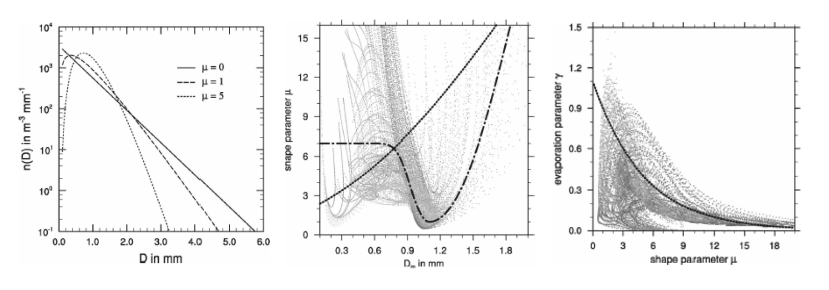
\includegraphics[scale=0.75]{./figure/mod_gamma_dist.eps}
\end{center}
\caption{Left figure shows the modified Gamma distribution for various shape parameters μm. Center figure shows the scatter plot of shape parameter and mean volume diameter for various initial conditions. Gray dots are from cloud model, dotted line is parameterization of Milbrandt and Yau (2005) and dashed-dotted line is that of Seifert (2008). Right figure shows the scatter plot of evaporation parameter and shape parameter. These are from Seifert (2008).}
\label{figsn2-17}
\end{figure}

\begin{figure}[htbp]
\begin{center}
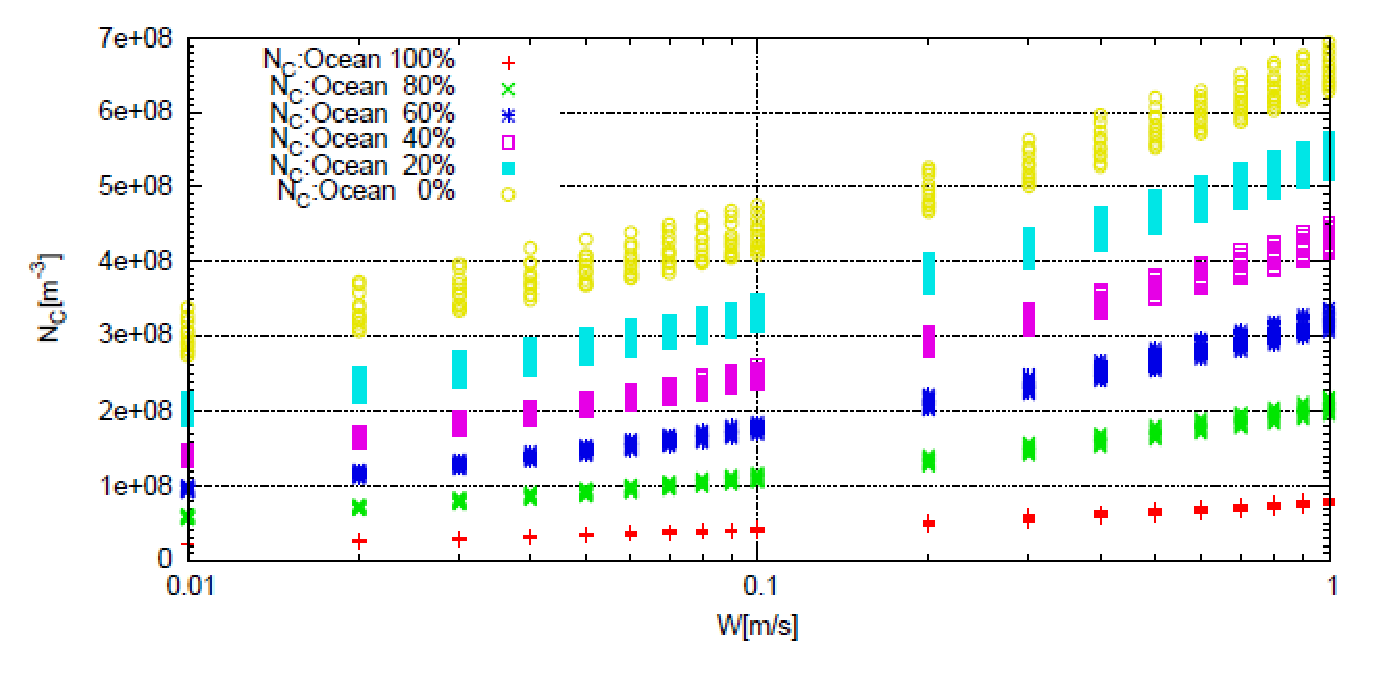
\includegraphics[scale=0.5]{./figure/density_max_num.eps}
\end{center}
\caption{Dependency of maximum number concentration on updraft velocity in ascending air parcel. These are based on a Twomey equation with various CCN conditions. Aerosol activation spectrum refers to eq.\ref{sn107}.}
\label{figsn2-18}
\end{figure}

\begin{figure}[htbp]
\begin{center}
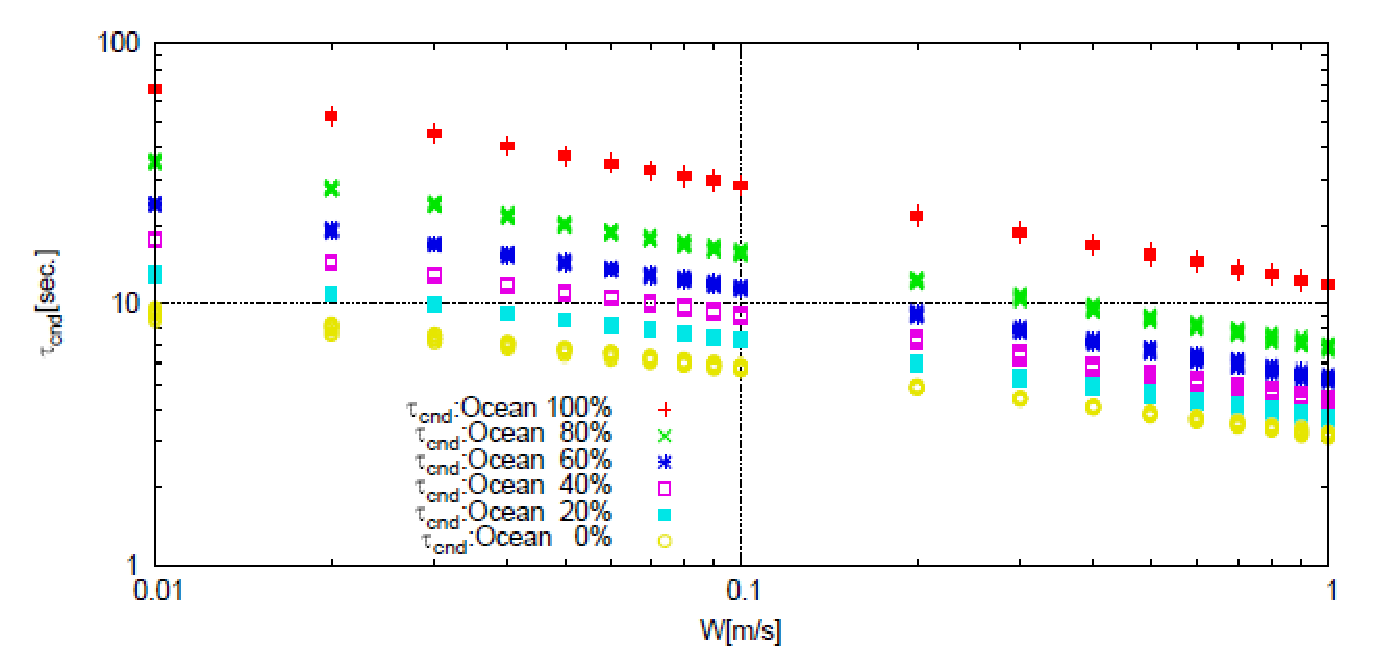
\includegraphics[scale=0.5]{./figure/cond_timescale.eps}
\end{center}
\caption{Timescale of condensation for cloud droplets at maximum number concentration in ascending air parcel. Experimental design is the same as Fig.\ref{figsn2-18}.}
\label{figsn2-19}
\end{figure}

\begin{figure}[htbp]
\begin{center}
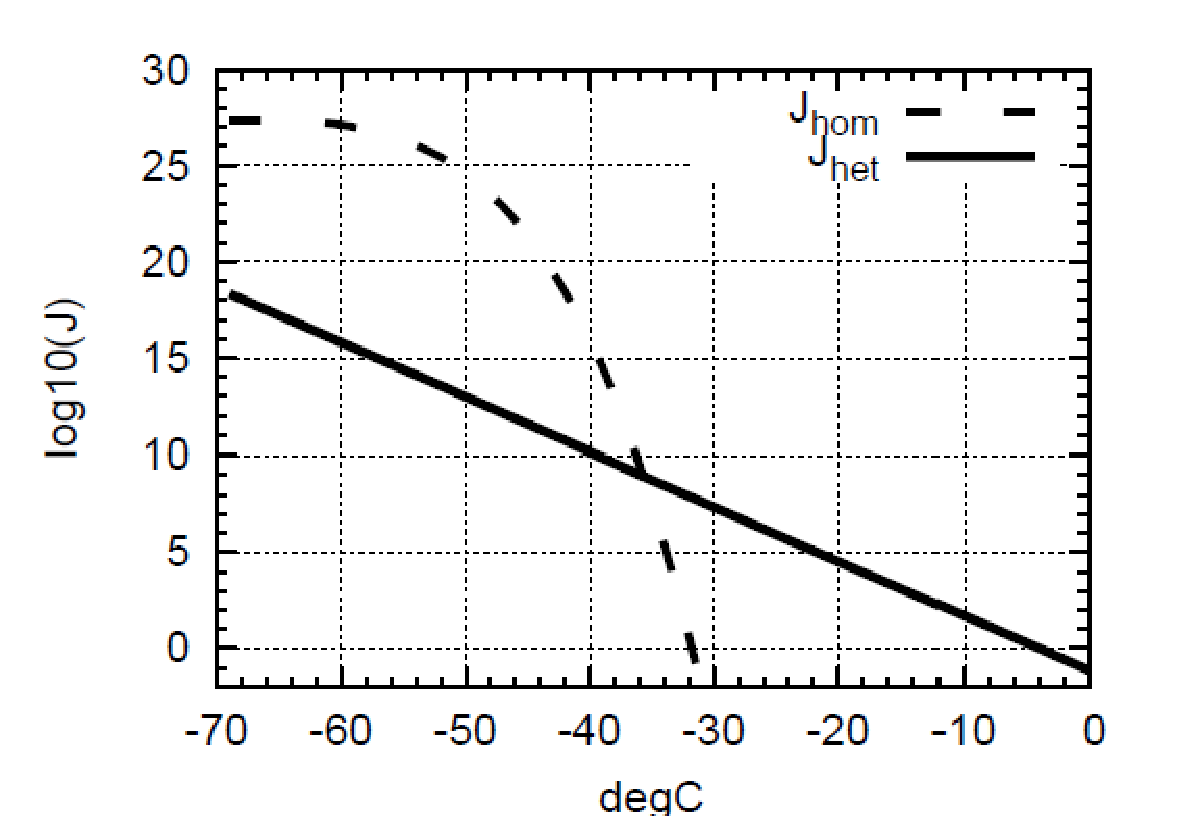
\includegraphics[scale=0.5]{./figure/homo_frz_rate.eps}
\end{center}
\caption{The dependencies of the homogeneous freezing rate (dashed line) and the heterogeneous freezing rate (solid line) on centigrade temperature. The freezing rates are in common logarithmic scale.}
\label{figsn2-20}
\end{figure}

\begin{figure}[htbp]
\begin{center}
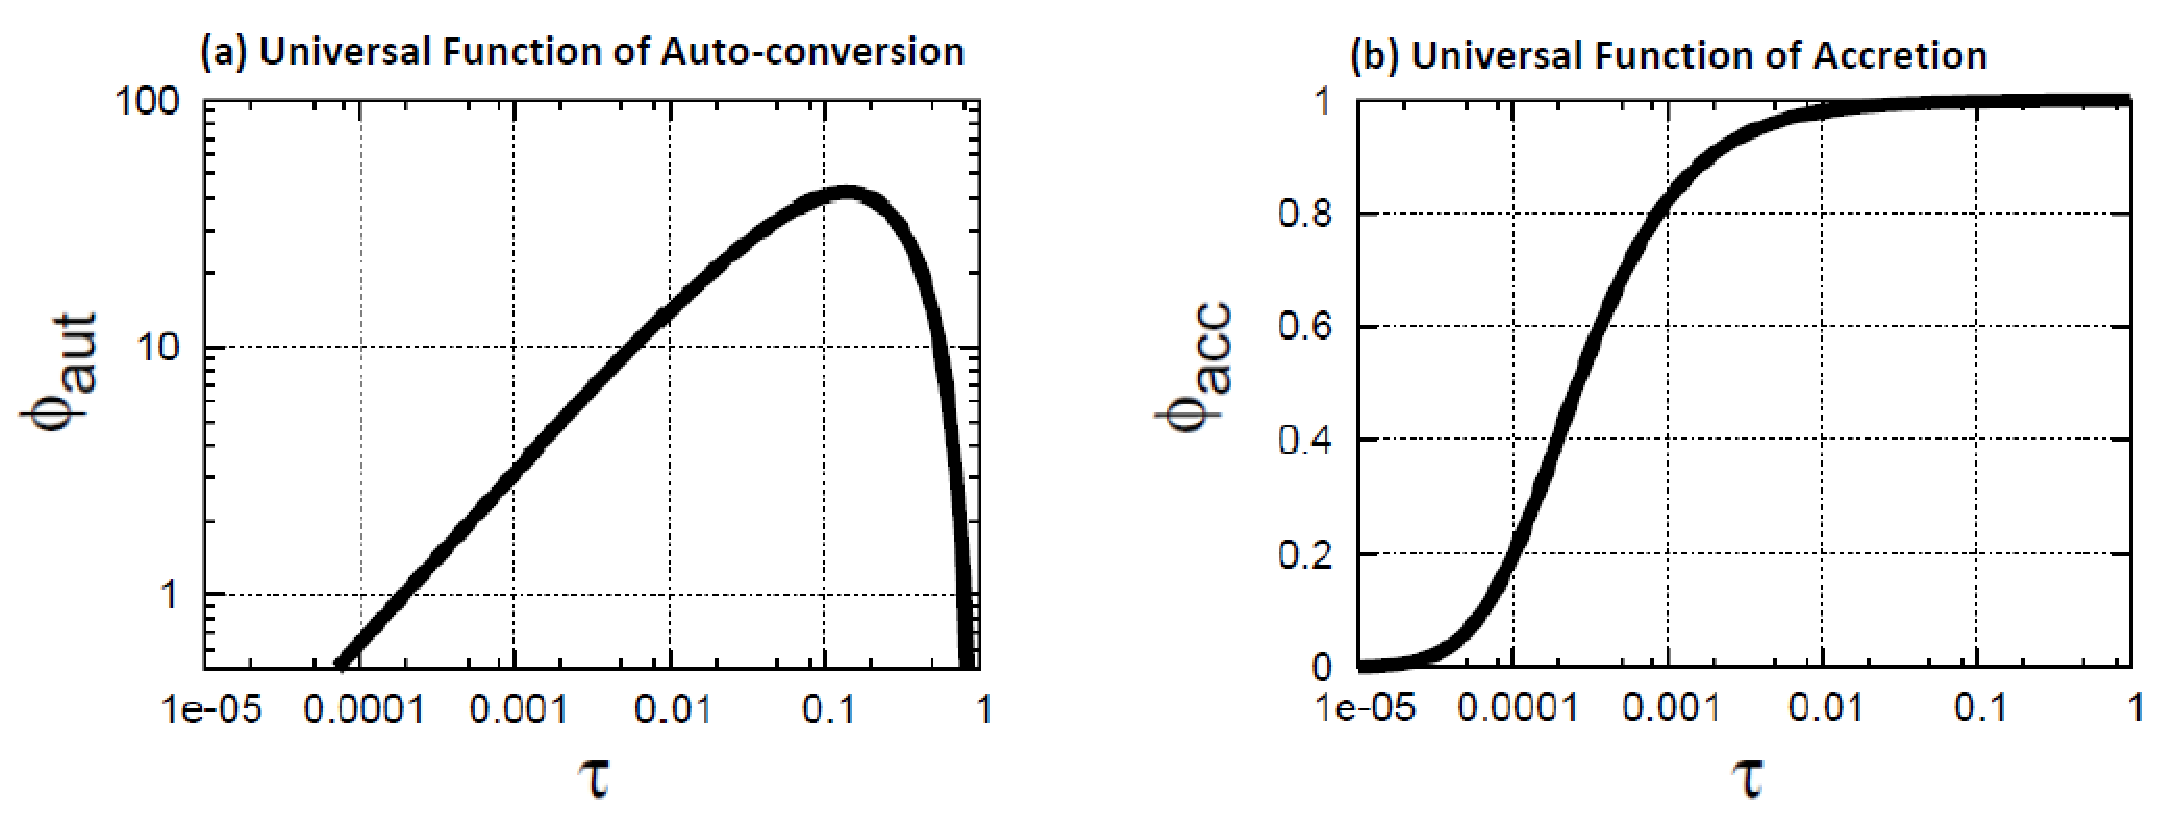
\includegraphics[scale=0.25]{./figure/univ_function.eps}
\end{center}
\caption{The universal functions of (a) auto-conversion and (b) accretion as a function of the dimensionless internal time scale.}
\label{figsn2-21}
\end{figure}

\begin{figure}[htbp]
\begin{center}
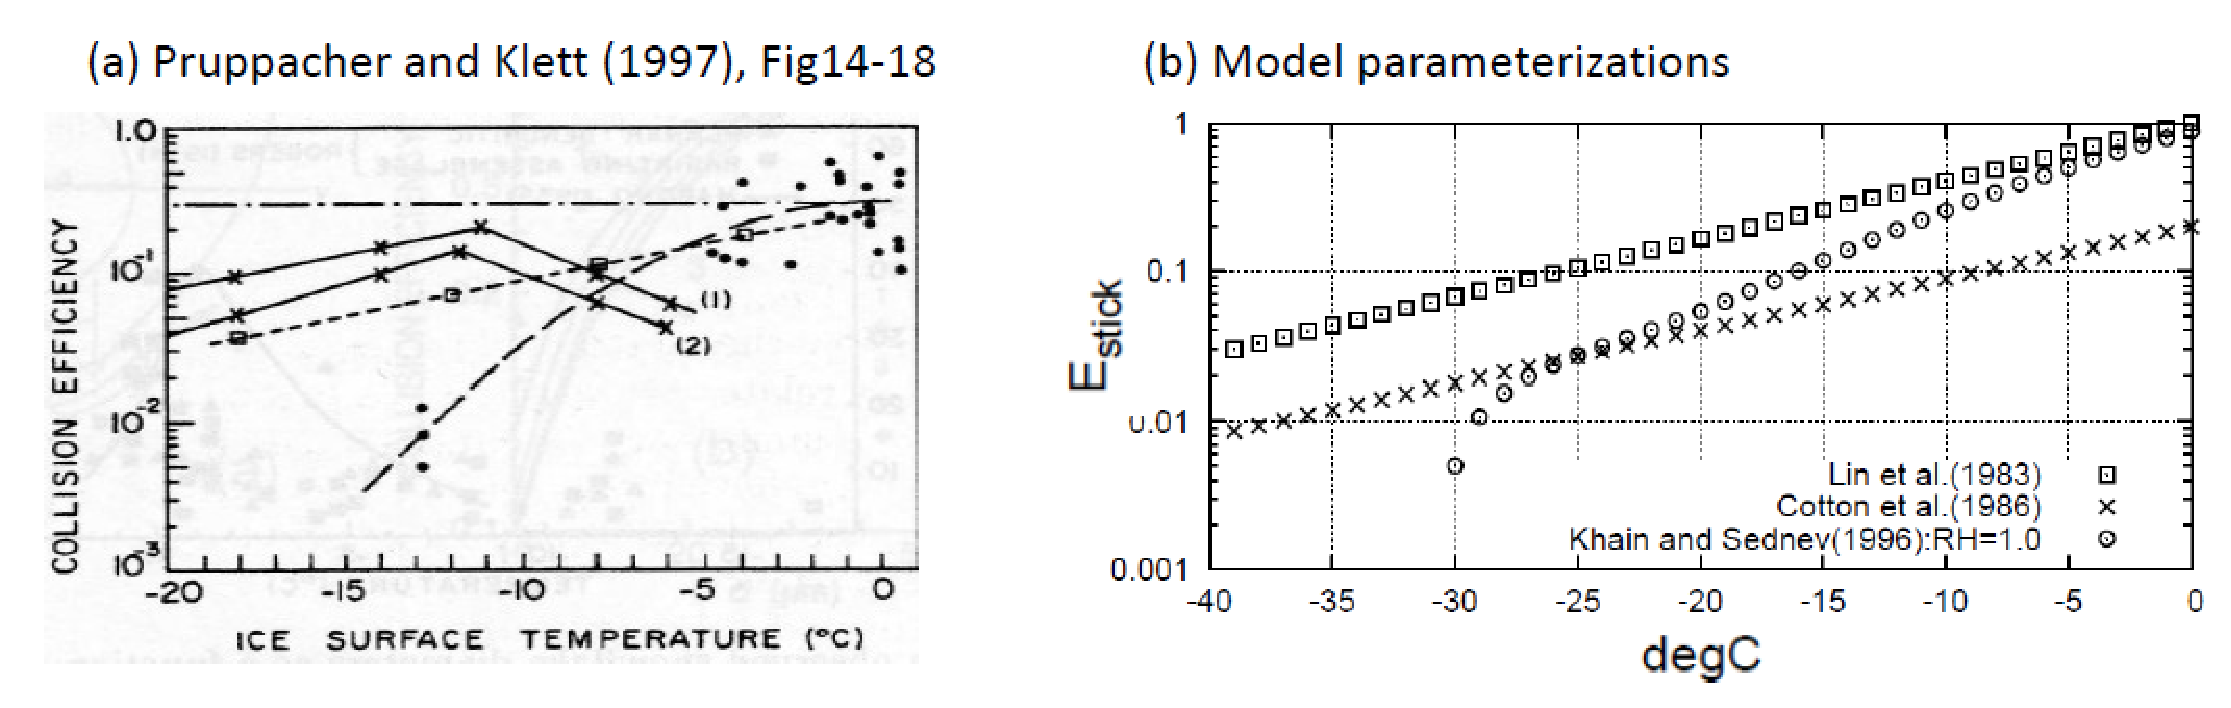
\includegraphics[scale=0.25]{./figure/stic_effic.eps}
\end{center}
\caption{The dependency of stick efficiencies on centigrade temperature. The stick efficiencies by (a) the various observations from Pruppacher and Klett (1997) and (b) model parameterizations.}
\label{figsn2-22}
\end{figure}

\begin{figure}[htpb]
\begin{center}
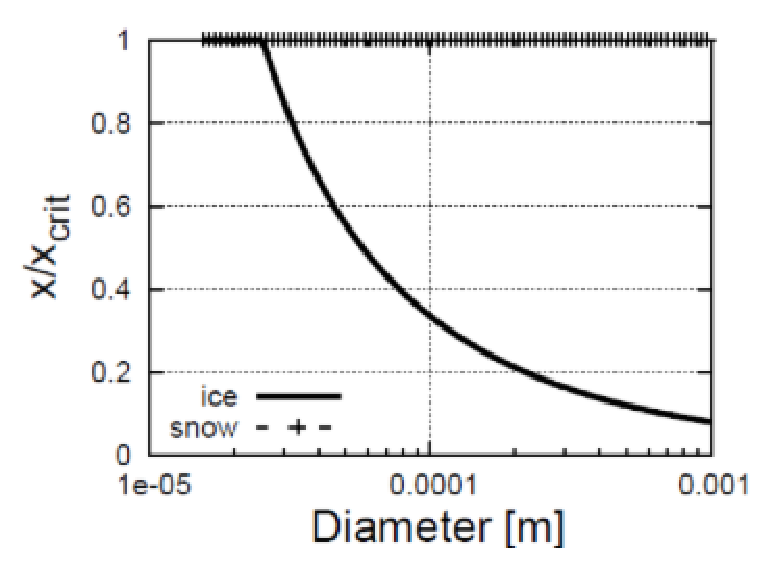
\includegraphics[scale=0.5]{./figure/partial_conversion_coef.eps}
\end{center}
\caption{The coefficients of partial conversion. Solid line shows the coefficient of ice, and the line with symbol shows the coefficient of snow.}
\label{figsn2-23}
\end{figure}

\subsubsection{Appendix of Seiki and Nakajima (2014)}
\subsubsection{The k-th moment of generalized Gamma distribution}
The kth moment of the DSD frequently appear in the equations of cloud microphysics. In this section, derivation of the kth moment of the generalized Gamma distribution is described. The generalized Gamma distribution is defined as $f(x) = \alpha x \nu exp(-\lambda x \mu)$. There are four parameters in this generalized Gamma distribution but only two prognostic moments in a CRM; the number concentration N and mass concentration L. Hence $\mu$ and $\nu$ are set constant parameters so that the other coefficients $\alpha$ and $\lambda$ can be related to N and L as follows.

\begin{eqnarray}
M^{0}=N&=&\alpha\int_{0}^{\infty}x^{\nu}exp(\lambda x^{\mu})dx\nonumber\\
&=&\frac{\alpha}{\lambda^{(\nu+1)/\mu}\mu}\int_{0}^{\infty}y^{(\nu+1)/\mu-1}exp(-y)dy,\;(y\equiv\lambda x^{\mu})\nonumber\\
&=&\frac{\alpha}{\lambda^{(\nu+2)/\mu}\mu}\Gamma\bigl(\frac{\nu+1}{\mu}\bigr)\label{sn255}\\
M^{1}=L&=&\frac{\alpha}{\lambda^{(\nu+2)/\mu}\mu}\Gamma\bigl(\frac{\nu+1}{\mu}\bigr)\nonumber
\end{eqnarray}

Then $\alpha$ is expressed as,

\begin{eqnarray}
\alpha=\frac{N\mu\lambda^{(\nu+1)/\mu}}{\Gamma\bigl(\frac{\nu+1}{\mu}\bigr)}=\frac{L\mu \lambda^{(\nu+2)/\mu}}{\Gamma\bigl(\frac{\nu+2}{\mu}\bigr)}\nonumber
\end{eqnarray}

and then we can derivev $\lambda$ and $\alpha$,

\begin{eqnarray}
\lambda=\Bigl[\frac{\Gamma\bigl(\frac{\nu+1}{\mu}\bigr)}{\Gamma\bigl(\frac{\nu+2}{\mu}\bigr)}\Bigr]^{-\mu}\bar{x}^{-\mu}\;\;and\;\;\alpha=\frac{\nu N}{\Gamma\bigl(\frac{\nu+1}{\mu}\bigr)}\lambda^{(\nu+1)/\mu}\label{sn256}
\end{eqnarray}

where $\bar{x}=L/N$ define the mean particle mass. Here we can rewrite the generalized Gamma distribution by using N and L in following form,

\begin{eqnarray}
f(x)=\frac{N}{\bar{x}}\bigl(\frac{x}{\bar{x}}\bigr)^{\nu}\frac{\mu}{\Gamma\bigl(\frac{nu+1}{\mu}\bigr)}\Bigl[\frac{\Gamma\bigl(\frac{\nu+2}{\mu}\bigr)}{\Gamma\bigl(\frac{\nu+1}{\mu}\bigr)}\Bigr]^{\nu+1}\exp\Bigl[-\bigl[\frac{\Gamma((\nu+2)/\mu)}{\Gamma((\nu+1)/\mu)}\frac{x}{\bar{x}}\bigr]^{\mu}\Bigr]\label{sn257}
\end{eqnarray}

The kth moment of DSD is now given by the expansion of eq.\ref{sn255} and by using eq.\ref{sn256},

\begin{eqnarray}
M^{k}=\frac{\Gamma\bigl(\frac{k+\nu+1}{\mu}\bigr)}{\Gamma\bigl(\frac{\nu+1}{\mu}\bigr)}\Bigl[\frac{\Gamma\bigl(\frac{\nu+1}{\mu}\bigr)}{\Gamma\bigl(\frac{\nu+2}{\mu}\bigr)}\Bigr]^{k}N\bar{x}^{k},\;\;(k\in R)
\end{eqnarray}


\subsection{Spectral Bin Model(SBM)\cite{suzuki_etal_2010}}
The Spectral Bin Model (SBM) was developed by Suzuki et al. (2010)\cite{suzuki_etal_2010}. The model forecasts Size Distribution Function(SDF) of 7 types hydrometeors (liquid, plate-ice, columner-ice, dendrite-ice, snow, graupel, and hail). \\
The SBM calculates mass density of the 7 types of hydrometeor and 1 type of aerosol as their SDFs. The SDF of aerosol can be changed by advection and acvitvaiton (i.e. nucleation from aerosol to cloud) process. The SDF of hydrometeors can be changed by several growth processes (i.e. activation from aerosol to cloud, condensation/evaporation, collision/coaguration, freezing/melting, ice nucleation, riming, aggregation, advection, and gravitational falling). \\
The time evolution of SDF (number density) of aerosol ($f_{a}(m,t)$) and SDF (number density) of hydrometeor ($f_{c}(m,t)$) are shown as equations:

\begin{eqnarray}
\frac{\partial f^{(\mu)}_{c}(m,t)}{\partial t}&=&Adv\bigl[f^{(\mu)}_{c}(m,t)\bigr]+Grav\bigl[f^{(\mu)}_{c}(m,t)\bigr]+\Bigl[ \frac{\partial f^{(\mu)}_{c}(m,t)}{\partial t}\Bigr ]_{cloud\;microphysics}\label{s10-1}\\
\frac{\partial f_{a}(m_{a},t)}{\partial t}&=&Adv\bigl[f_{a}(m_{a},t)\bigr]+Grav\bigl[f_{a}(m_{a},t)\bigr]+\Bigl[ \frac{\partial f_{a}(m_{a},t)}{\partial t} \Bigr ]_{cloud\;microphysics}.\label{s10-2}
\end{eqnarray}

where $\mu$ shows type of hydrometeor (the 7 types), $Adv[]$, $Grav[])$ shows change of SDF by the advection and the gravitational falling. $\Bigl[ \Bigr]_{cloud\;microphycis}$ shows changes of SDF by the cloud microphysical processes.\\
The time evolution of $f_{c}^{(\mu)}(m,t)$ and $f_{a}(m,t)$ are shown as:

\begin{eqnarray}
\Bigl[ \frac{\partial f_{c}^{(\mu)}(m,t)}{\partial t}\Bigl]_{cloud\;microphysics}&=&\Bigl[\frac{\partial f_{c}^{(\mu)}(m,t)}{\partial t}\Bigr]_{activation}+\Bigl[\frac{\partial f_{c}^{(\mu)}(m,t)}{\partial t}\Bigr]_{cond/evap}\nonumber\\
&+&\Bigl[\frac{\partial f_{c}^{(\mu)}(m,t)}{\partial t}\Bigr]_{coll/coag/rim/agg}\nonumber\\
&+&\Bigl[\frac{\partial f_{c}^{(\mu)}(m,t)}{\partial t}\Bigr]_{frz}+\Bigl[\frac{\partial f_{c}^{(\mu)}(m,t)}{\partial t}\Bigr]_{melt}\nonumber\\
\Bigl[ \frac{\partial f_{a}(m_{a},t)}{\partial t}\Bigl]_{cloud\;microphysics}&=&\Bigl[\frac{\partial f_{a}(m_{a},t)}{\partial t}\Bigr]_{activation}\nonumber
\end{eqnarray}

where $\Bigl[\;\Bigr]_{***}$ show change of SDF by each cloud growth processes. The detail of these processes will be shown later.\\
 The change of SDFs by advection and gravitational falling (i.e. first and second term of eq. \ref{s10-1}, and \ref{s10-2}  ) are calculated by dynamical core of SCALE-RM shown in section 3.


\subsubsection{Discretization of Size Distribution Function(SDF)}
The SDF of aerosol and cloud is predict as mass density of each particle size ($g_{a}(m_{a})$, $g_{c}^{(\mu)}(m)$). However most of equations are given as equations of number density of cloud/aerosol ($f_{c}^{(\mu)}(m,t)$, $f_{a}(m_{a},t)$), the mass density of cloud/aerosol are transferred to number density of cloud/aerosol ($g_{a}(m_{a},t)=m_{a}g_{a}(m_{a},t)$, $g_{c}^{(\mu)}(m,t)=m^{(\mu)}f_{c}^{(\mu)}(m,t)$).\\
To cover wide size range (i.e. $2\;\mu m$ $\sim$ $3\;mm$), logarithmically uniform grid system ($log(m)\equiv \eta$, $log(m_{a})\equiv \eta_{a}$) is used. In this system, the relationship, $\frac{m_{i+1}}{m_{i}}=const.$ is satisfied.

\subsubsection{Activation from aerosol to cloud particles (Nucleation process)}
The change of SDFs by activation from aerosol to cloud particles are calculated based on Kohler theory (Kohler 1936). Through this process, aerosols whose radii are larger than critical radius of aerosol ($r_{a,crit}$) are activated to clouds. The critical radius is given as

\begin{eqnarray}
r_{a,crit}=\bigl( \frac{4}{27}\frac{A^{3}}{B}\frac{1}{S_{w}}\Bigr )^{1/3}, \:\:\:A=\frac{2\sigma}{R_{v}\rho_{L}T},\:\:\: B=i_{v}\frac{M_{v}}{M_{s}}\frac{\rho_{s}}{\rho_{L}}.\label{s10-3}
\end{eqnarray}

where $S_{w}$, $\sigma$, $R_{v}$, $\rho_{L}$, $T$, $i_{v}$, $M_{v}$, $M_{s}$, $\rho_{s}$ show supersaturation of water, surface tention of water, gas constant of vapor, temperature, van't Hoff factor ($=2$), moleculer weight of water, moleculer weight of aerosol, and density of aerosol, respectively.\\
At each time step, $r_{a,crit}$ are calculated by using temperature, and mass of aerosols whose radii are larger than $r_{a,crit}$ remove from SDF of aerosol and they are transferred to SDF of cloud as newly generated cloud particles.\\
The radii of newly generated clouds are corresponding to those of aerosols, but if the radii of aeorol are smaller than the lower limit of cloud SDF, the radii of newly generated clouds are set to smallest size of cloud SDF ($\sim 2 \mu m$).\\
The change of aerosol's SDF and hydrometeor's SDF are shown as:

\begin{eqnarray}
\Bigl[\frac{\partial f_{a}}{\partial t}\Bigr]_{activation}&=&-\int_{m_{a,crit}}^{\infty}f_{a}(m_{a},t)dm_{a}\label{s10-4}\\
\Bigl[\frac{\partial f_{c}^{(\mu)}}{\partial t}\Bigr]_{activation}&=&-\Bigl[\frac{\partial f_{a}}{\partial t}\Bigr]_{activarion}\label{s10-5}
\end{eqnarray}

where $m_{a,crit}=\bigl(=\frac{4\pi}{3}r_{a}^{3}\rho_{a}$ is mass of aerosol particles whose radii are the same as critical radii, $r_{a,crit}$. When there are not enough vapor to activate all aerosol particles whose radii are larger than the critical radius, i.e.

\begin{eqnarray}
\int_{m_{a,crit}}^{\infty}m_{a}f_{a}(m_{a},t)dm_{a} > q_{v}\rho,\label{s10-6}
\end{eqnarray}

only the aerosol particles whose radii are larger than $r_{a0,crit}$, which are given as:

\begin{eqnarray}
\int_{m_{a0,crit}}^{\infty}m_{a}f_{a}(m_{a},t)dm_{a} = q_{v}\rho,\label{s10-7}
\end{eqnarray}


are transferred to cloud paricles as:

\begin{eqnarray}
\Bigl[\frac{\partial f_{a}}{\partial t}\Bigr]_{activation}&=&-\int_{m_{a0,crit}}^{\infty}f_{a}(m_{a},t)dm_{a},\label{s10-8}\\
\Bigl[\frac{\partial f_{c}^{(\mu)}}{\partial t}\Bigr]_{activation}&=&-\Bigl[\frac{\partial f_{a}}{\partial t}\Bigr]_{activarion}.\label{s10-9}
\end{eqnarray}

where $q_{v}$ and $\rho$ is mixing ratio of water vapor and density.

\subsubsection{Condensation/Evaporation}
Calculation of condensation and evaporation process are based on a equation. The mass change by these two process are given by an equation (e.g. Rogers and Yau, 1989\cite{ry_1989}):

\begin{eqnarray}
\frac{dm}{dt}&=&C^{(\mu)}(m)G^{(\mu)}(T)S^{(\mu)}\\
G^{(\mu)}(T)&=&
\left\{
\begin{array}{l}
G_{w}(T)\;\;\;(\mu : \:liquid)\\
G_{i}(T)\;\;\;(\mu : \:ice)
\end{array}\right. \nonumber\\
G_{w}(T)&=&\frac{4\pi}{\frac{R_{v}T}{e_{w}(T)D_{v}}+\frac{L_{w}}{KT}\bigl( \frac{L_{w}}{R_{v}T}-1\Bigr )}\nonumber\\
G_{i}(T)&=&\frac{4\pi}{\frac{R_{v}T}{e_{i}(T)D_{v}}+\frac{L_{i}}{KT}\bigl( \frac{L_{i}}{R_{v}T}-1\Bigr )}\nonumber\\
S^{(\mu)}&=&
\left\{
\begin{array}{l}
S_{w}\;\;\;(\mu : liquid)\\
S_{i}\;\;\;(\mu : ice)
\end{array}\right.\nonumber
\end{eqnarray}

where $C^{(\mu)}(m)$ is capasitance, which depends on shape of each types of hydrometeor, $S_{w}$, $S_{i}$ are super saturation of water and ice, $L_{w}$, $L_{i}$ is sensible heat of evaporation, sublimation, $D_{v}$ is diffusion constant of vapor, $K$ is conductivity of air, and $e_{w}$, $e_{i}$ is saturation vapor pressure and saturation ice pressure, respectively. Condensation (evaporation) occur when $S^{(\mu)}$ is positive (negative).\\
To calculate change of SDF by condensation/evaporation, mass flux ($F^{(\mu)}_{cond/evap}$) on each bin is given by using number density ($f_{c}^{(\mu)}$) and $\frac{dm}{dt}$ as:

\begin{eqnarray}
F^{(\mu)}_{cond/evap}=f^{(\mu)}(m)\frac{dm}{dt}=f^{(\mu)}(m)C^{(\mu)}G^{(\mu)}(T)S^{(\mu)}.\label{s10-10}
\end{eqnarray}

Using this equation, time evolution of SDF ($f^{(\mu)}$) is given as

\begin{eqnarray}
\Bigl[\frac{\partial f^{(\mu)}(m,t)}{\partial t}\Bigr]_{cond/evap}&=&-\frac{\partial}{\partial m}F^{(\mu)}_{cond/evap}(m)\nonumber\\
&=&-\frac{\partial}{\partial m}\bigl (f^{(\mu)}(m)C^{(\mu)}\bigr ) G^{(\mu)}(T)S^{(\mu)}.\label{s10-11}
\end{eqnarray}


By using the $\eta(=\log(m))$, the eq.\ref{s10-11} is transferred to advection equation :

\begin{eqnarray}
\frac{\partial f^{(\mu)}(\eta)}{\partial t}&=&-\frac{\partial}{\partial \eta}\bigl ( f^{(\mu)}(\eta)U^{(\mu)}(\eta)\bigr)\label{s10-12}\\
U^{(\mu)}(\eta)&=&\frac{C^{(\mu)}(\eta)}{\exp (\eta)}G^{(\eta)}(T)S^{(\eta)}.\nonumber
\end{eqnarray}

To solve the eq. \ref{s10-12}, a scheme developed by Bott (1989)\cite{bott_1989} is used. The number density of i-th bin after $\Delta t$ ($f_{i}(t+\Delta t)$) is given as follow:

\begin{eqnarray}
f_{i}(t+\Delta t)&=&f_{i}(t)-\frac{\Delta t}{\Delta \eta}\bigl [F_{cond/evap,i+1/2}-F_{cond/evap,i-1/2}\Bigr ].\nonumber\\
F_{cond/evap,i+1/2}&=&\frac{\Delta \eta}{\Delta t}\Bigl[ \frac{i^{+}_{l,i+1/2}}{i_{l,j}}f_{i}(t)-\frac{i^{-}_{l,i+1/2}}{i_{l,i+1}}f_{i+1}(t)\Bigr ]\nonumber\\
i^{+}_{l,i+1/2}&=&max\bigl(0,I^{+}_{l}(c_{i+1/2})\bigr)\nonumber\\
i^{-}_{l,i+1/2}&=&max\bigl(0,I^{-}_{l}(c_{i+1/2})\bigr)\nonumber\\
i^{+}_{l,i}&=&max\bigl(I_{l,i},i^{+}_{l,i+1/2}+i^{-}_{l,i+1/2})\bigr)\nonumber\\
I^{+}_{l}(c_{i+1/2})&=&\sum_{k=0}^{2}\frac{a_{i,k}}{(k+1)2^{k+1}}\bigl[1-(1-2c^{+}_{j})^{k+1}\bigr]\nonumber\\
I^{-}_{l}(c_{i+1/2})&=&\sum_{k=0}^{2}\frac{a_{i+1,k}}{(k+1)2^{k+1}}(-1)^{k}\bigl[1-(1-2c^{-}_{j})^{k+1}\bigr]\nonumber\\
a_{i,0}&=&-\frac{1}{24}\bigl( f_{i+1}(t)-26f_{i}(t)+f_{i-1}(t) \bigr)\nonumber\\
a_{i,1}&=&\frac{1}{2}\bigl( f_{i+1}(t)-f_{i-1}(t) \bigr)\nonumber\\
a_{i,2}&=&\frac{1}{2}\bigl( f_{i+1}(t)-2f_{i}(t)+f_{i-1}(t) \bigr)\nonumber\\
c_{i}^{\pm}&=&\pm\bigl( c^{n}_{i+1/2}\pm | c^{n}_{i+1/2}|\bigr )/2\nonumber\\
c^{n}_{i+1/2}&=&U^{n}_{i+1/2}\frac{\Delta t}{\Delta \eta}
\end{eqnarray}

Since the super saturation ($S^{(\mu)}$) can change during time step ($\Delta t$), we apply a method shown below to reflect the change of supersaturation during $\Delta t$.\\
Time evolution of supersaturation can be given by equations:

\begin{eqnarray}
\frac{d}{dt}\left(
\begin{array}{l}
S_{w}\\
S_{i}\\
\end{array}\right )
&=&
\left(
\begin{array}{cc}
a_{c/e}& b_{c/e}\\
c_{c/e}& d_{c/e}
\end{array}\right)
\left(
\begin{array}{l}
S_{w}\\
S_{i}
\end{array}\right)
=
A
\left(
\begin{array}{l}
S_{w}\\
S_{i}
\end{array}\right)\label{s10-13}\\
a_{c/e}&=&-(S_{w}+1)\Bigl(\frac{1}{q_{v}}+\frac{L_{w}}{R_{v}T^{2}}\frac{L_{w}}{C_{p}}\Bigr )\int f^{(w)}(m)C^{(w)}(m)dm G_{w}(t)\nonumber\\
b_{c/e}&=&-(S_{w}+1)\Bigl(\frac{1}{q_{v}}+\frac{L_{w}}{R_{v}T^{2}}\frac{L_{i}}{C_{p}}\Bigr ) \sum_{\mu \in ice}\int f^{(\mu)}(m)C^{(\mu)}(m)dm G_{i}(t)\nonumber\\
c_{c/e}&=&-(S_{i}+1)\Bigl(\frac{1}{q_{v}}+\frac{L_{i}}{R_{v}T^{2}}\frac{L_{w}}{C_{p}}\Bigr ) \int f^{(w)}(m)C^{(w)}(m)dm G_{w}(t)\nonumber\\
d_{c/e}&=&-(S_{i}+1)\Bigl(\frac{1}{q_{v}}+\frac{L_{i}}{R_{v}T^{2}}\frac{L_{i}}{C_{p}}\Bigr ) \sum_{\mu \in ice}\int f^{(\mu)}(m)C^{(^mu)}(m)dm G_{i}(t)\nonumber
\end{eqnarray}


where $q_{v}$ is mixing ration of vapor. \\
Using eigen value of $A$ ($\Lambda_{+}$, $\Lambda_{-}$ ($\Lambda_{+}>\Lambda_{-})$), and assuming $a_{c/e}$, $b_{c/e}$, $c_{c/e}$, $d_{c/e}$ is constant during $\Delta t$, average value of super saturation ($\bar{S}_{w,i}(t)$) during $\Delta t$ is given as:

\begin{eqnarray}
\bar{S}_{w}(t)=\frac{1}{\Delta t}\int_{t}^{t+\Delta t}S_{w}(\tau)d\tau&=&b\frac{e^{\Lambda_{+}\Delta t}-1}{\Lambda_{+}\Delta t}S_{+}(t)+b\frac{e^{\Lambda_{-}\Delta t}-1}{\Lambda_{-}\Delta t}S_{-}(t)\nonumber\\
\bar{S}_{i}(t)=\frac{1}{\Delta t}\int_{t}^{t+\Delta t}S_{i}(\tau)d\tau&=&(\Lambda_{+}-a)\frac{e^{\Lambda_{+}\Delta t}-1}{\Lambda_{+}\Delta t}S_{+}(t)+(\Lambda_{-}-a)\frac{e^{\Lambda_{-}\Delta t}-1}{\Lambda_{-}\Delta t}S_{-}(t)\nonumber\\
S_{+}(t)&=&\frac{(\Lambda_{-}-a)S_{w}(t)-bS_{i}(t)}{b(\Lambda_{-}-\Lambda_{+})}\nonumber\\
S_{+}(t)&=&\frac{(a-\Lambda_{+})S_{w}(t)+bS_{i}(t)}{b(\Lambda_{-}-\Lambda_{+})}\nonumber
\end{eqnarray}

The averaged super saturation ($\bar{S}_{w,i}(t)$) is used to solve the eq. \ref{s10-13}.

\subsubsection{Collision/Coagulation/Riming/Aggregation}
Collision/Coagulation process are calculated by solving Stochastic Collision Equation (e.g. Pruppecher and Klett, 1997)\cite{pk_1997}:

\begin{eqnarray}
\frac{\partial f(m)}{\partial t}&=&\int_0^{m/2}f(m')f(m-m')K(m',m-m')dm' \nonumber\\
&-&f(m)\int_0^{\infty}f(m'')K(m,m'')dm''\label{s10-14}
\end{eqnarray}

where $K(m,m')$ is collection kernel function. Three types of the kernel function, i.e. Long type kernel (Long, 1974\cite{long_1974}), Golovin type kernel (Golovin, 1963\cite{golovin_1963}) and Hydro-dynamic dynamic kernel as shown eq. \ref{s10-15} are implemented into the SCALE-RM.

\begin{eqnarray}
K(m,m')=\pi(r(m)-r(m'))\left| V(m)-V(m')\right |E_{col}(m,m')E_{coag}(m,m')\label{s10-15}
\end{eqnarray}

where $r(m)$ is radius of hydrometeors whose mass is $m$, and $V(m)$ is terminal velocity of hydrometeors. The terminal velocity of each species of hydrometeor and each size are shown in Figure \ref{figs10-term} $E_{col}$, and $E_{coag}$ is collision effieiency and coagulation efficiansy, respectively.\\

\begin{figure}[ht]
\begin{center}
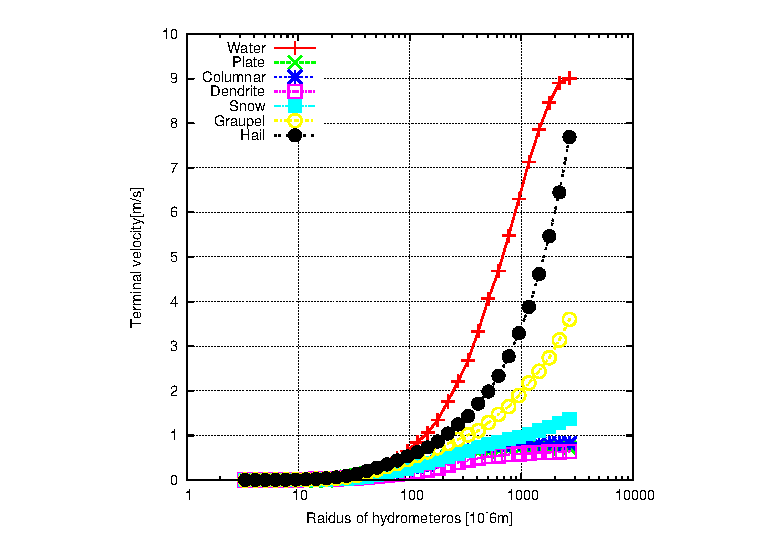
\includegraphics[scale=0.9]{./figure/terminal-velocity.eps}
\end{center}
\caption{Terminal velocity of Water (Plus), Plate-type ice (Cross), Columnar-type ice (Asterisk), Dendrite-type ice(Open square), Snow(Closed square), Graupel(Open circle), and Hail(Closed circle)}
\label{figs10-term}
\end{figure}


Although the stochastic collision equation can be apply for collision/coagulation of one type of hydrometeors (i.e. liquid water), the SCALE-RM predicts 7 types of hydrometeors, and interactions of these types hydrometeors (i.e. riming/aggregation) must be calculated. To calculate the interaction of all 7 types of hydrometeors, the extented stochastic collision equation:

\begin{eqnarray}
\Bigr[\frac{\partial f^{(\mu)}(m)}{\partial t}\Bigr]_{coll/coag/rim/agg}&=&\nonumber\\
\sum_{\lambda}\sum_{\nu}\int_{0}^{m/2}f^{(\lambda)}&(&m')f^{(\nu)}(m-m')K_{\lambda\nu}(m',m-m')dm' \nonumber\\
-f^{(\mu)}(m)\sum_{\kappa}\int_0^{\infty}f^{(\kappa)}&(&m'')K_{\kappa\mu}(m,m'')dm''\label{s10-16}
\end{eqnarray}

is applied (where $\mu$, $\nu$, $\lambda$, $\kappa$ represent species of hydrometeor). The convinations of $\mu$, $\nu$, $\lambda$ are shown in table \ref{table-s10-1}.

\begin{table}[h]
\begin{center}
\caption{Catalog of interaction between 7 species. W, I, S, G, H shows water, ice, snow, graupel, and hail, respectively. G/H shows graupel(hail) generates when T is lower(higher) than 270.15}
\label{table-s10-1}
\begin{tabular}{cccccc}
\hline
     & W   & I   & S   & G   & H   \\ \hline\hline
W    & W   & G/H & G/H & G/H & G/H \\ \hline
I    & I   & S   & S   & I   & I   \\ \hline
S    & S   & S   & S   & S   & S   \\ \hline
G    & G/H & G/H & G   & G   & G/H \\ \hline
H    & G/H & G/H & G/H & G/H & H   \\ \hline
\end{tabular}
\end{center}
\end{table}


To solve the stochastic collision equation, a scheme developed by Bott (1998)\cite{bott_1998} was implemented into SCLAE-RM.\\
The Bott (1998)\cite{bott_1998} scheme calculate evolution of mass density distribution ($g(\eta)=mf(\eta)$, $\eta=\log(m)$). The stochastic collision equation can be transferred to

\begin{eqnarray}
\frac{\partial g(\eta)}{\partial t}&=&\int_{\eta_{0}}^{\eta_{1}}\frac{m^{2}}{(m-m')^{2} m'}g(\eta-\eta') K(\eta-\eta',\eta')g(\eta')d\eta' \nonumber\\
&-&\int_{\eta_{0}}^{\infty} g(\eta)\frac{K(\eta,\eta')}{m'}g(\eta')d\eta'.\label{s10-17}
\end{eqnarray}

 where $\eta_{1}=\log(m/2)$. Decreases of mass of i-th bin and j-th bin are given by

\begin{eqnarray}
\frac{\partial g_{i}^{(\mu)}}{\partial t}=-\Delta g^{(\mu)}_{i} K_{\mu\nu}(i,j)\frac{g_{j}^{(\nu)}}{m_{j}}\Delta \eta\label{s10-18}
\end{eqnarray}

and


\begin{eqnarray}
\frac{\partial g_{j}^{(\mu)}}{\partial t}=-\Delta g^{(\nu)}_{j}K_{\mu\nu}(i,j)\frac{g_{i}^{(\mu)}}{m_{i}}\Delta \eta\label{s10-19}
\end{eqnarray}

respectively. The terms corresponds to the second term of right-hand side of eq.\ref{s10-17}. The eq. \ref{s10-18} and eq. \ref{s10-19} can transfer to

\begin{eqnarray}
\Delta g_{i}^{(\mu)}=g_{i}^{(\mu)}\Bigl [1-\exp\bigl(-K_{\mu\nu}(i,j)\frac{g^{(\nu)}_{j}}{m_{j}}\Delta \eta\Delta t\bigr) \Bigl]\label{s10-20}\\
\Delta g_{j}^{(\nu)}=g_{j}^{(\nu)}\Bigl [1-\exp\bigl(-K_{\mu\nu}(i,j)\frac{g^{(\mu)}_{i}}{m_{i}}\Delta \eta\Delta t\bigr) \Bigl].\label{s10-21}
\end{eqnarray}

The sum of $\Delta g_{i}^{(\mu)}$ and $\Delta g_{j}^{(\nu)}$ corresponds to newley generated mass by collision of hydrometeor whose mass is $m_{i}$ and $m_{j}$. The newly generated mass ($g'=\Delta g_{i}^{(\mu)}+\Delta g_{j}^{(\nu)}$, which is coresponding to first term of right-hand side of eq.\ref{s10-17}) added k-th bin ($m_{k}=m_{i}+m_{j}$). Since $m_{k}$ is not always bin center, newly generated mass is devided to k-th and k+1-th bin as follow.\\
The production of k-th and k+1-th bin is represened:

\begin{eqnarray}
\Delta g_{k}^{(\lambda)}&=&g_{k}^{\lambda}+g'-\zeta\label{s10-22}\\
\Delta g_{k+1}^{(\lambda)}&=&g_{k+1}^{\lambda}+\zeta\label{s10-23}\\
\zeta&=&\frac{g'}{g_{k}^{(\lambda)}+g'}\sum_{s=0}^{2}\frac{a_{k,s}}{(s+1)2^{k+1}}[1-(1-2c_{k})^{k+1}]\nonumber\\
c_{k}&=&\frac{m'-m_{k}}{m_{k+1}-m_{k}}\nonumber\\
a_{k,0}&=&-\frac{1}{24}(g_{k+1}^{(\lambda)}-26g_{k}^{(\lambda)}+g_{k-1}^{(\lambda)})\nonumber\\
a_{k,1}&=&-\frac{1}{2}(g_{k+1}^{(\lambda)}-g_{k-1}^{(\lambda)})\nonumber\\
a_{k,2}&=&-\frac{1}{2}(g_{k+1}^{(\lambda)}-2g_{k}^{(\lambda)}+g_{k-1}^{(\lambda)})\nonumber
\end{eqnarray}

These procedure is applied for all bin of all types of hydrometeors.\\
In addition, to calculate this process fastly, a scheme of Sato et al. (2009)\cite{sato_etal_2009} are also implemented into SCALE-RM.

\subsubsection{Freezing}
The calculation of freezing process is based on a parameterization of Bigg (1953)\cite{bigg_1953}. The parameterization is calculated number density of water ($f_{c}^{(w)}$), wchich can be freezed:

\begin{eqnarray}
\frac{\partial}{\partial t}f^{(w)}(m)&=&-\frac{f^{(w)}(m)}{\tau_{fr}}\label{s10-24}\\
\tau_{fr}&=&\frac{\exp \bigl[b_{fr}(T_{0}-T)\bigr]}{a_{fr} m}\nonumber
\end{eqnarray}

where $a_{fr}=10^{-4}s^{-1}$, and $b_{fr}=0.66^{o}C^{-1}$ are emperical parameters, and $T_{0}$ is 273.15 $K$.\\
The eq. \ref{s10-24} can transfer to

\begin{eqnarray}
\frac{\partial g^{(w)(m)}}{\partial t}&=&-\frac{g^{(w)}(m)}{\tau_{fr}(m)}\\
\tau_{fr,i}&=&\frac{\exp\bigl (b_{fr}(T_{0}-T)\bigr )}{a_{fr}m}\nonumber
\end{eqnarray}

From this equation, The mass change of i-th bin during $\Delta t$ is given as

\begin{eqnarray}
g_{i}^{(w)}(t+\Delta t)=g_{i}^{(w)}-Frz_{i}\\
\left \{
\begin{array}{r}
g_{i}^{(plate)}(t+\Delta t)=g_{i}^{(plate)}+Frz_{i}\:\:\: (r_{w}<200\mu m)\\
g_{i}^{(hail)}(t+\Delta t)=g_{i}^{(hail)}+Frz_{i}\:\:\: (r_{w}>200\mu m)
\end{array} \right.\label{s10-26}\\
Frz_{i}=g_{i}^{(w)}(t)\Bigl [1-\exp\bigl (-\frac{\Delta t}{\tau_{fr,i}}\bigr )\bigr]\nonumber
\end{eqnarray}


 As shown in eq. \ref{s10-26}, the mass of liuid is transfer from to plate type ice ($r_{w}<200\mu m$) or hail ($r_{w}>200\mu m$).

\subsubsection{Melting}
The calculation of melting process is too simple way, that is, all ice particles (i.e. plate, columner, dendrite, snow, graupel and hail) melt immediately when the temperature is larger than $T_{0}=273.15$ $K$. This is too simply to represent ice phase process, and we will modify this method near future.


\subsection{Kessler Parameterization}
SCALE implements a one-moment bulk microphysical scheme, which treats only warm clouds (cloud and rain). This scheme predicts the mixing ratio of cloud ($Q_{cloud}$) and rain ($Q_{rain}$). Cloud microphysical processes treated in this scheme are saturation adjustment (corresponding to nucleation, evaporation, and cloud condensation), evaporation, auto-conversion, accretion, and sedimentation. The tendency of $Q_{cloud}$, $Q_{rain}$, and $Q_{v}$ (vapor mixing ratio) is as follows:

\begin{eqnarray}
\frac{\partial Q_{cloud}}{\partial t}&=&dQ|_{sat}-dQ|_{auto}-dQ|_{acc}\\
\frac{\partial Q_{rain}}{\partial t}&=&dQ|_{auto}+dQ|_{acc}-dQ|_{evap}-F_{Q_{r}}|_{sed}\\
\frac{\partial Q_{v}}{\partial t}&=&dQ|_{evap}-dQ|_{sat}
\end{eqnarray}

where $dQ|_{sat}$, $dQ|_{auto}$, $dQ|_{acc}$, and $dQ|_{evap}$ represent the mixing ratio tendency by saturation adjustment, auto-conversion, accretion, and evaporation, respectively. $F_{Q_{r}}|_{sed}$ represents flux of $Q_{r}$ by sedimentation.\\ $dQ|_{auto}$, $dQ|_{acc}$, and $dQ|_{evap}$ are given as:

\begin{eqnarray}
dQ_{auto}&=&\left\{
\begin{array}{ll}
Q_{cloud}*10^{-3} & (Q_{cloud}>10^{-3})\\
0 & (else)\\
\end{array}\right.\\
dQ_{acc}&=&2.2\times Q_{cloud}\times Q_{rain}^{0.875}\\
dQ_{evap}&=&\left\{
\begin{array}{ll}
f_{vent} \frac{q_{s}-Q_{cloud}}{q_{s}\rho}\frac{(\rho*Q_{rain})^{0.525}}{5.4\times 10^{5}+\frac{2.55\times 10^{8}}{pq_{s}}} & ( q_{s} > Q_{cloud})\\
0 & (else)\\
\end{array} \right.
\end{eqnarray}

where $f_{vent}$ is the ventilation factor ($f_{vent}=1.6+124.9(\rho Q_{rain})^{0.2046}$), and the unit of $dQ_{***}$ is [kg/kg/s]. $p$, $q_{s}$, and $\rho$ are pressure, saturation vapor mixing ratio, and total density, respectively.\\
$dQ|_{sat}$ is given as:

\begin{eqnarray}
dQ|_{sat}=Q_{v}-q_{s}.
\end{eqnarray}

Terminal velocities of cloud ($V_{t,c}$) and rain ($V_{t,r}$) are given as:

\begin{eqnarray}
V_{t,c}&=&0\\
V_{t,r}&=&36.34(\rho Q_{rain})^{0.1364} [m/s]
\end{eqnarray}



\subsection{Double-Moment Bulk \cite{sn_2014}}

\subsubsection{Treatment of hydrometeors}
Generally, characteristics of cloud particles are determined by their size, shape, and the chemical properties of solute within them. Representation of these characteristics requires a multi-dimensional parameter space of size, shape, and chemical compositions. Since development of a cloud resolving model (CRM) coupled with an aerosol transport model is beyond the scope of this study, we consider a two-dimensional parameter space of size and shape of cloud particles. We then categorize cloud models into two major groups, according to their representation of cloud particles. One is the bin method, using discretized particle size bins and predicting the population density of particles in each bin. The other is the bulk method, in which particle size distributions are approximated by several prescribed modes, predicting the total populations of particles of each mode. The treatment of hydrometeors adopted in this study is described in the following sections.

\subsubsection{Droplet Size Distribution}
The Seiki and Nakajima (2014)\cite{sn_2014} scheme is designed to maintain the self-consistency of assumptions regarding droplet size distribution (DSD) and the shapes of ice particles among cloud microphysical processes. Following Seifert and Beheng (2006; hereafter, SB06), Seiki and Nakajima(2014)\cite{sn_2014} predict the moments of the DSD of each hydrometeor, assuming generalized gamma distribution to analytically formulate cloud microphysics, as follows:

\begin{eqnarray}
f_{a}(r)=\alpha_{a}x^{\nu_{a}}\exp(-\lambda x)
\label{sn7}
\end{eqnarray}

where the index a $\in$ (c,r,i,s,g) represents cloud water, rain, cloud ice, snow, and graupel. For a given DSD, the k-th moment can be defined as follows:

\begin{eqnarray}
M^{(k)}_{a}\equiv \int_{0}^{\infty}x^{k}f_{a}(r)dx,\;\;(k\in {\bf R})
\label{sn8}
\end{eqnarray}

For example, the 0-th moment of a DSD is the number concentration $N_{a}$, and the 1st moment is the mass concentration $L_{a} = \rho q_{a}$. The evolution of DSD is represented by updating $\alpha_{a}$ and $\lambda_{a}$ using $N_{a}$ and $L_{a}$ with two fixed parameters, $\nu_{a}$ and $\mu_{a}$, respectively. The diagnostic parameters $\alpha_{a}$ and $\lambda_{a}$ are calculated as follows:

\begin{eqnarray}
\alpha_{a}=\frac{\mu_{a}\lambda_{a}}{\Gamma\Bigl(\frac{\nu_{a}+1}{\mu_{a}}\Bigr)}\lambda_{a}^{\frac{\nu_{a}+1}{\mu_{a}}}\\
\label{sn9}
\lambda_{a}=\Bigl[\frac{\Gamma\Bigl(\frac{\nu_{a}+1}{\mu_{a}}\Bigr)}{\Gamma\Bigl(\frac{\nu_{a}+2}{\mu_{a}}\Bigr)}\Bigr]^{-\nu_{a}}\nonumber
\end{eqnarray}

with mean particle mass $\bar{x}\equiv L_{a}/N_{a}$. We maintain the self-consistency of the shape of ice particles by assuming power law relationships between: 1) particle mass and maximum dimension D, and 2) particle mass and projected area to flow A, as follows:

\begin{eqnarray}
D&=&a_{m}x^{b_{m}}\\
\label{sn10}
A&=&a_{ax}x^{b_{m}}
\label{sn11}
\end{eqnarray}

where $a_{m}$, $b_{m}$, $a_{ax}$, and $b_{ax}$ are constant coefficients. We chose to use constant parameters for DSD representation, following SB06 for cloud water, cloud ice, snow, and graupel, and following Seifert (2008) for rain (assuming collisional-breakup equilibrium conditions). The shapes of ice particles are those given by Mitchell (1996), assuming cloud ice as hexagonal plates, snow as assemblages of planar polycrystals in cirrus clouds, and graupel as lump graupel. The above-mentioned constant parameters for each hydrometeor are summarized in Table \ref{table_sn14-1}.

\begin{table}[h]
\begin{center}
\caption{Constant parameters chosen for the generalized gamma distribution; power law coefficients used for maximum dimensions and projected area, and ranges of lower- and upper limits of mean mass.}
\label{table_sn14-1}
\scalebox{0.85}{
\begin{tabular}{cccccc}
\hline
                         & cloud water   & rain    & cloud ice   & snow   & graupel   \\ \hline\hline
$\nu$                    & 1  & -1/3 & 1 & 1 & 1 \\ \hline
$\mu$                    & 1  &  1/3 & 1/3   & 1/3   & 1/3   \\ \hline
$a_{m}$[m $kg^{-bm}$]    & 0.124   & 0.124   & 1.24   & 1.24   & 0.346   \\ \hline
$b_{m}$                  & 1/3 & 1/3 & 0.408   & 0.408   & 0.357 \\ \hline
$a_{ax}$[$m^{2}$$kg^{-bA}$]    & 0.0121   & 0.0121   & 0.178   & 0.196   & 0.0599   \\ \hline
$b_{ax}$ & 2/3 & 2/3 & 0.755   & 0.768   & 0.714 \\ \hline
$\bar{x_{min}}[kg]$ & $4.2\times 10^{-12}$ & $4.2\times 10^{-12}$ & $4.2\times 10^{-12}$ & $4.2\times 10^{-12}$ & $4.2\times 10^{-12}$ \\ \hline
$\bar{x_{max}}[kg]$ & $2.6\times 10^{-10}$ & $2.6\times 10^{-10}$ & $2.6\times 10^{-10}$ & $2.6\times 10^{-10}$ & $2.6\times 10^{-10}$ \\ \hline
\end{tabular}
}
\end{center}
\end{table}

\subsubsection{Terminal velocity of hydrometeors}
In the same manner as Seifert and Beheng (2006a), the terminal velocities of particles are formulated in power laws, except for gravitational sedimentation, which is described using an accurate formula because it is directly compared with precipitation data. The terminal velocities of hydrometeors are determined by the balance between drag and gravitational forces. Traditionally, the terminal velocities for small spherical particles with small Reynolds number ($N_{Re}$) are described by Stokes’ Law:

\begin{eqnarray}
\nu_{t,stokes}(r)=\frac{2g(\rho_{w}-\rho)}{9\eta_{a}}r^{2}
\label{sn12}
\end{eqnarray}

where $g$ = 9.80616 $[m s^{-2}]$ is gravitational acceleration, $\rho w$ = 1000 $kg m^{-3}$ is the density of liquid water, $\rho$ is the density of air, and $\eta_{a}$ is the dynamic viscosity of air. Laboratory experiments have shown that terminal velocity departs from Stokes’ Law as the Reynolds number increases (Gunn and Kinzer, 1948; Beard and Pruppacher, 1969). Other formulas are thus required for larger droplets, such as rain droplets and ice crystals.\\
In the case of liquid water droplets, terminal velocity can be determined well by laboratory experiments because of the simplicity of shape. In contrast, there are many observed terminal velocities of ice particles for various shapes of ice crystals. Bohm (1989), Bohm (1992), and Mitchell (1996) proposed general formulations of the terminal velocities of ice particles based on the boundary layer theory, with their studies showing good agreement with observational data. In this study, we calculated terminal velocities for each ice particle based on Mitchell (1996) and then created a fitting curve using a power law within a suitable diameter range. \\
In theoretical formulas, the terminal velocities of hydrometeors are dependent on diameter, shape, the Reynolds number, and the Best (or Davies) number ($N_{X}$). Applying these to cloud microphysics is extremely complicated; here, we therefore apply a simplified approach suggested by Beard (1980):\\
1. The terminal velocity is calculated for the reference atmosphere.\\
2. The terminal velocity in the atmosphere is adjusted from the reference value.\\
In the following paragraphs, we describe terminal velocities for the reference atmosphere and the adjustment technique.

\subsubsection{Terminal velocity of liquid water droplets for the reference atmosphere}
In the case of liquid water droplets, absence of shape variability makes formulation easier than in the case of ice particles. Here, we only consider dependency on the diameter of droplets. Seifert and Beheng (2006) applied the formulation of Rogers et al. (1993), the analytical approximation of Gunn and Kinzer’s (1948) observation data:

\begin{eqnarray}
\nu_{t}(D)=
\left\{
\begin{array}{l}
a_{R_{s}}D(1-exp(-b_{R_{s}}D)),\;\;(D<D_{0,r}) \\
a_{R_{l}}-b_{R_{l}}exp(-c_{R_{l}}D),\;\;(D>D_{0,r}) \\
\label{sn13}
\end{array}
\right.
\end{eqnarray}

where $a_{R_{s}}= 4000 s^{-1}$, $b_{R_{s}}=12000 m^{-1}$, $a_{R_{l}}=9.65 m s^{-1}$, $b_{R_{l}} = 10.43 m s^{-1}$, $c_{R_{l}} = 600 m^{-1}$, and $D_{0}$, $r=7.45\times10^{-4}$ m. This formulation approaches the quadratic form of Stokes’ Law in the limit for small diameters. In addition, Gunn and Kinzer’s (1948) data agrees well with the terminal velocities calculated via theoretical formulation based on the boundary layer theory (Bohm, 1992). We therefore applied eq.\ref{sn13} for rain sedimentation (Fig. \ref{figsn2-11}2 11). Here, the reference atmosphere of the formulation is $T = 293 K$, $p = 1000hPa$, and relative humidity is 0.5 (Gunn and Kinzer, 1948).

\subsubsection{Terminal velocity of solid water particles for the reference atmosphere}
In the case of ice particles, we derive the theoretical formulation of the terminal velocity based on Mitchell (1996). In general the aerodynamic drag force $F_{D}$ on a particle is expressed as follows:

\begin{eqnarray}
F_{D}\equiv \frac{1}{2}\rho\nu_{t}^{2}AC_{D}
\label{sn14}
\end{eqnarray}

where $C_{D}$ is the drag coefficient. Terminal velocity is determined by the equilibrium condition between the drag force and gravitational acceleration:

\begin{eqnarray}
\nu_{t}=\bigl(\frac{2xg}{\rho AC_{D}}\bigr)^{1/2}
\label{sn15}
\end{eqnarray}

The problem of derivation of the terminal velocity is reduced to derivation of the drag coefficient, independent of the terminal velocity. In practice, Mitchell (1996) and many other researchers calculated the terminal velocity by defining the Best number ($N_{X}$), as follows:

\begin{eqnarray}
N_{x}\equiv C_{D}N_{R_{e}}^{2}=\frac{2xg\rho D^{2}}{A\eta_{a}^{2}}
\label{sn16}
\end{eqnarray}

where $N_{R_{e}}$ is the Reynolds number. The terminal velocity can be calculated after the relationship between Best and Reynolds numbers is determined. In the relationship, it is convenient for the drag coefficient to be determined by the Reynolds number, although the dependency of the former is complicated. A theoretical formulation of the drag coefficient was proposed by Abraham (1970). The drag coefficient is the dimensionless number defined by the drag force, the dynamic pressure, and the projection area of the particle (see eq.\ref{sn14}). Abraham (1970) assumed that the effective projection area of the particle contained the projection area of the particle itself and also the boundary layer surrounding the particle, as follows:


\begin{eqnarray}
F_{D}=\frac{1}{2}\rho \nu_{t}^{2}C_{0}A\bigl(1+\frac{\delta_{b}}{r_{A}}\bigl)^{2}
\label{sn17}
\end{eqnarray}

where $C_{0}$ is the drag coefficient due to the pressure of the fluid and should be determined independently of the shape, $\delta_{b}$ is the boundary layer depth, and $r_{A}$ is the radius of a circle with the equivalent projection area. Furthermore, the ratio of boundary layer depth to radius is expressed as follows:

\begin{eqnarray}
\frac{\delta_{b}}{r_{A}}=\frac{\delta_{0}}{N_{R_{e}}^{1/2}}
\label{sn18}
\end{eqnarray}

where $\delta_{0}$ is a non-dimensional constant. Substituting eq.\ref{sn18} into eq.\ref{sn17}, the drag coefficient, which also includes the effect of the boundary layer, corresponds to the following:

\begin{eqnarray}
C_{D}=C_{0}\bigl(1+\frac{\delta_{0}}{N_{R_{e}}^{1/2}}\bigr)^{2}
\label{sn19}
\end{eqnarray}

The drag coefficient is thus expressed by the Reynolds number. The relationship between Reynolds and Best numbers is derived by substituting eq.\ref{sn19} into eq.\ref{sn16}:

\begin{eqnarray}
N_{R_{e}}=\frac{\delta_{0}^{2}}{4}\Bigl[\bigr(1+\frac{4N_{X}^{1/2}}{\delta_{0}^{2}C_{0}^{1/2}}\bigr)^{1/2}-1 \bigr]^{2}
\label{sn20}
\end{eqnarray}

Here we use $C_{0}$ = 0.6 and $\delta_{0}$ = 5.83, as provided by Bohm (1989). Finally the terminal velocity of ice particles is calculated by substituting eq.\ref{sn16} and eq.\ref{sn20} into the definition of the Reynolds number:

\begin{eqnarray}
\nu_{t}&=&\frac{N_{Re}\eta_{a}}{D\rho}\nonumber\\
&=&\frac{\eta_{a}}{D\rho}\frac{\delta_{0}^{2}}{4}\Bigl[\bigl[1+\frac{4}{\delta_{0}^{2}C_{0}^{1/2}}\bigr(\frac{2xg\rho D^{2}}{A\eta_{a}^{2}}\bigl)^{1/2}\bigr]^{1/2}-1\Bigr]^{2}
\label{sn21}
\end{eqnarray}

In this formulation, required variables are mass, projection area, maximum dimension of ice particles, and thermodynamical variables. Here we use several piecewise-constant mass-maximum dimension, and projection area-maximum dimension relationships provided by Mitchell (1996). The terminal velocities of various ice particles are plotted in Fig.\ref{figsn2-12}. As shown in Fig.\ref{figsn2-11}, there is less difference between hexagonal plates and stellar crystals with broad arms with diameter less than a few hundred micrometers. We therefore only consider hexagonal columns and hexagonal plates as representative of the ice category.


\subsubsection{Adjustment factor of terminal velocity}
Beard (1980) suggested that calculation of the terminal velocity using the Best number could be simplified with use of an adjustment factor ($f_{vt}$), defined as:

\begin{eqnarray}
\nu_{t}=\nu_{t0}f_{vt}
\label{sn23}
\end{eqnarray}

where $v_{t0}$ is a reference terminal velocity. He demonstrated that $f_{vt}$ was not sensitive to the shape of hydrometeors. When electrical force is not considered in cloud microphysics, formulas of $f_{vt}$ are as follows:

\begin{eqnarray}
f_{vt}&=&f_{vt0}\;\;(N_{Re_{0}}\leq0.2)\label{sn24}\\
f_{vt}&=&f_{vt\infty}\;\;(N_{Re_{0}}\geq1000)\label{sn25}\\
f_{vt}&=&f_{vt0}\nonumber\\
&+&(f_{vt\infty}-f_{vt0})(1.61+lnN_{R_{e}0})/8.52\;\;(N_{Re_{0}}<1000)\label{sn26}\\
f_{vt0}&\equiv&(\eta_{0}/\eta)\label{sn27}\\
f_{vt\infty}&\equiv&(\rho_{0}/\rho)^{0.5}\label{sn28}\\
N_{R_{e}0}&\equiv&\rho_{0}Dv_{t0}/\eta_{0}\label{sn29}
\end{eqnarray}

The upper ( $N_{R_{e}}$ = 1000 ) and lower ( $N_{R_{e}}$ = 0.2 ) limits of the Reynolds number correspond to diameters of several millimeters and tens of micrometers, respectively. Seifert and Beheng (2006) applied a further simplified adjustment factor based on eqs.\ref{sn27} and \ref{sn28}, as follows:

\begin{eqnarray}
f_{vt,n}=(\rho_{0}/\rho)^{\gamma_{n}}, \;\;\;(n=c,r,i,s,g)
\label{sn30}
\end{eqnarray}

where $\gamma_{c}$ = 1.0 and $\gamma_{r}$ = $\gamma_{i}$ = $\gamma_{s}$ = $\gamma_{g}$ = 0.5 This simplified formula of the adjustment factor is intended to avoid dependency on the Reynolds number. However, $\gamma_{n}$ = 0.5 is only valid for high Reynolds number particles with diameters > several millimeters, as shown in eq.\ref{sn21}. The above formula therefore always underestimates the terminal velocity of cirrus clouds. Another simplified formula for cirrus clouds was suggested by Heymsfield and Iaquinta (2000), as follows:

\begin{eqnarray}
f_{vt}=(p/p_{0})^{-0.178}(T/T_{0})^{-0.394}
\label{sn31}
\end{eqnarray}

where $T_{0}$ = 233 K and $p_{0}$ = 300 hPa. By using these adjustment factors, we can only consider the terminal velocity for the reference atmosphere. Adjustment factors used for each hydrometeor in this study are summarized in Table \ref{table_sn14-2-8}:

\begin{table}[h]
\begin{center}
\caption{Adjustment factor for the reference terminal velocity.}
\label{table_sn14-2-8}
\scalebox{0.75}{
\begin{tabular}{cccccc}
\hline
           & cloud     & rain    & ice   & snow   & graupel   \\ \hline\hline
$f_{vt}$   & 1         & $(\rho_{0}/\rho)^{0.5}$ & $(p/p_{0})^{-0.178}(T/T_{0})^{-0.394}$ & $(p/p_{0})^{-0.178}(T/T_{0})^{-0.394}$ & $(p/p_{0})^{-0.178}(T/T_{0})^{-0.394}$ \\ \hline
\end{tabular}
}
\end{center}
\end{table}


\subsubsection{Weighted mean terminal velocity}
In gravitational sedimentation, mean terminal velocity weighted by the k-th moments of DSD (${\bf \bar{v_{k,nq}}}$) is calculated in a straightforward manner, as follows:

\begin{eqnarray}
\bar{v_{k,nq}}=\int_{0}^{\infty}x^{k}f_{nq}(x)v_{t,nq}(x)dx
\label{sn32}
\end{eqnarray}

However, the terminal velocity formulas, eqs.\ref{sn14} and \ref{sn21}, are too complicated to analytically integrate eq.\ref{sn32}. Seifert and Beheng (2006) and Seifert (2008) used the large branch of eq.\ref{sn14} for rain droplets and simple power laws derived by observation for other hydrometeors. Here, we provide more accurate formulations to calculate weighted terminal velocities.\\
As shown above, dependency of the terminal velocity on diameter varies across aerodynamical regimes. In other words, dependency varies with diameter range. We therefore first prepared two branches of the terminal velocities of hydrometeors (except for cloud droplets) so as to integrate DSDs analytically. For cloud droplets, we used the same power law provided by Seifert and Beheng (2006), based on Stokes’ law. For rain droplets, we directly used the formulation of eq.\ref{sn14}, which allows analytical integration of each branch. In contrast, we need to derive two fitting curves for ice particles. The formulation of the terminal velocity of ice particles is described as a power law of the diameter using the least-square method, as follows:

\begin{eqnarray}
v_{t,js}&=&a_{v,js}x^{b_{v,js}},\;\;(js=i,s,g)\label{sn33}\\
(RMSE)_{k,js}&=&\sum_{id=1}^{id_max}\bigl(ln\bar{v_{k,js,true}}(\bar{D_{id}})-ln\bar{v_{k,js}}(\bar{D_{id}})\bigr)^{2}\label{sn34}\\
\frac{\partial(RMSE)_{k,js}}{\partial a_{v,js}}&=&0,\:\frac{\partial (RMSE)_{k,js}}{\partial b_{v,js}}=0\nonumber\\
\bar{v_{k,js}}(\bar{D_{id}})&=&\int_{0}^{\infty}a_{v,js}x^{b_{v,js}+k}f(x,\bar{D_{id}},L)dx/L\nonumber\\
&=&a_{v,js}\frac{\Gamma\bigl(\frac{v_{js}+b_{v,js}+k+1}{\mu_{js}}\bigr)}{\Gamma\bigl(\frac{v_{js}+k+1}{\mu_{js}}\bigr)}
\Bigl[\frac{\Gamma\bigl(\frac{v_{js}+1}{\mu_{js}}\bigr)}{\Gamma\bigl(\frac{v_{js}+2}{\mu_{js}}\bigr)}\Bigr]^{b_{v,js}}\bar{x_{id,js}^{b_{v,js}}}\label{sn35}\\
\bar{v_{k,js,true}}(\bar{D_{id}})&=&\sum_{i=1}^{imax}x^{k}v_{t,js,true}f_{logD}(lnD_{i},\bar{D_{id}},L)\Delta ln D/L\nonumber
\end{eqnarray}

where $D_{1}=10\mu m$, $D_{imax}=10mm$, $i_{max}=1000$, and L is an arbitrary constant. The fitting ranges of the mean volume diameter in eq.\ref{sn34} are from 20 to 400 $\mu$m for the small branch and from 200 to 2000 $\mu m$ for the large branch. The derived parameters are summarized in Table \ref{table_sn14-2-9}.\\
Second, the terminal velocity with a certain mean diameter is calculated by interpolating between the two branches in the logarithmic scale of the diameter. We use the mean diameter weighted by the kth moments of DSD in the interpolation. The formulation of weighted terminal velocities of rain droplets and solid particles are as shown below:

\begin{eqnarray}
\bar{v_{k,nq}}&=&w_{k,nq}\bar{v_k,lrg,nq}+(1-w_{k,nq})\bar{v_{k,lrg,nq}},\;\;(nq=r,i,s,g)\label{sn36}\\
w_{k,r}&=&0.5(1+tanh(\pi ln(\bar{D_{k,r}}/D_{0,k,r})))\nonumber\\
w_{k,js}&=&max(0.0, \;min(1.0,0.5(1+ln(\bar{D_{k,js}}/D_{0,k,js}))))\;\;(js=i,s,g)\nonumber\\
\bar{D_{k,nq}}&=&\frac{\int_{0}^{\infty}D_{nq}(x)x^{k}f_{nq}(x)dx}{\int_{0}^{\infty}x^{k}f_{nq}(x)dx}\nonumber\\
              &=&\bar{D_{nq}}\frac{\Gamma\bigl(\frac{v_{nq}+b_{m,nq}+k+1}{\mu_{nq}}\bigr)}{\Gamma\bigl(\frac{v_{nq}+k+1}{\mu_{nq}}\bigr)}\Bigl[\frac{\Gamma\bigl(\frac{v_{nq}+1}{/mu_{nq}}\bigr)}{\Gamma\bigl(\frac{v_{nq}+2}{\mu_{nq}}\bigr)}\Bigr]^{b_{m,nq}}\label{sn37}\\
\bar{v_{k,sml,r}}&=&\frac{f_{vt,r}}{M_{r}^{k}}\int_{0}^{\infty}\bigl[a_{R_{s}}D(1-exp(-b_{R_{s}}D))\bigr]x^{k}N_{r}(D)dD\nonumber\\
&=&a_{R_{s}}\frac{(1+\mu_{D,r}+3k)}{\lambda_{D,r}}\nonumber\\
&\times&\Bigl[1-\bigl(1+\frac{b_{R_{s}}}{\lambda_{D,r}}\bigr)^{-2-\mu_{D,r}-3k}\Bigr]\bigl(\frac{\rho_{0}}{\rho}\bigr)^{1/2}\label{sn38}\\
\bar{v_{k,lrg,r}}&=&\frac{f_{vt,r}}{M_{r}^{k}}\int_{0}^{\infty}\bigl[a_{Rl}-b_{Rl}exp(-c_{Rl}D)\bigr]x^{k}N_{r}(D)dD\nonumber\\
&=&a_{Rl}-b_{Rl}\bigl(1+\frac{c_{Rl}}{\lambda_{D,r}}\bigr)^{-1-\mu_{D,r}-3k}\bigl(\frac{\rho_{0}}{\rho}\bigr)^{1/2}\label{sn39}\\
N_{r}(D)&=&N_{0,r}D^{-\mu_{D,r}}exp(-\lambda_{D,r}D)
\end{eqnarray}

where $D_{0,r}$ and $D_{0,js}$ are the branch points of the fitting curves (see Table \ref{table_sn14-2-10}). Here we apply the form of the modified gamma distribution for diameter as a DSD of rain droplets. Derivation and correspondences of the coefficient $N_{0,r}$, the slope parameter $\lambda_{D}$,$r$, and shape parameter $\mu D$ appearing in the modified gamma distribution are described in Appendix B. Weighted terminal velocities of ice particles for two branches are calculated by eq.\ref{sn35}. Fig.\ref{figsn2-13} shows the terminal velocity of rain droplets weighted by number and mass concentration. Our method gives better results than those obtained using the approximated method adopted by Seifert and Beheng (2006) in the range within their upper and lower limits. Fig.\ref{figsn2-14} shows terminal velocities of ice particles weighted by number and mass concentration.


\begin{table}[h]
\begin{center}
\caption{Coefficients and exponents of the relationship between mass and terminal velocity of each hydrometeor used in gravitational sedimentation and other processes.}
\label{table_sn14-2-9}
\scalebox{0.5}{
\begin{tabular}{cccccc}
\hline
Hydrometeors & Sedimentation of mass & Sedimentation of mass & Sedimentation of number   & Sedimentation number & other process   \\ \hline\hline
             & Small                 & Large                 & Small                     & Large                 &                 \\ \hline
Cloud        & $a_{v}=3.75\times10^{5},b_{v}=2/3$ & $a_{v}=3.75\times10^{5},b_{v}=2/3$ & $a_{v}=3.75\times10^{5},b_{v}=2/3$ & $a_{v}=3.75\times10^{5},b_{v}=2/3$ & $a_{v}=3.75\times10^{5},b_{v}=2/3$ \\  \hline
Rain         & \ref{sn14}            & \ref{sn14}            & \ref{sn14}                & \ref{sn14}           & \ref{sn14}      \\ \hline
Hexagonal plate & $a_{v}=5800,b_{v}=0.505$ & $a_{v}=167,b_{v}=0.325$ & $a_{v}=1.24\times10^{5},b_{v}0.549$ & $a_{v}=422,b_{v}=0.385$ & $a_{v}=5800,b_{v}=0.505$\\ \hline
Hexagonal columns & $a_{v}=2900,b_{v}=0.466$ & $a_{v}=32.2,b_{v}=0.224$ & $a_{v}=9698,b_{v}0.531$ & $a_{v}=64.2,b_{v}=0.274$ & $a_{v}=2900,b_{v}=0.466$\\ \hline
Aggregates of planar polycrystals & $a_{v}=1.52\times10^{5},b_{v}=0.528$ & $a_{v}=306.0,b_{v}=0.330$ & $a_{v}=2.93\times10^{5},b_{v}0.567$ & $a_{v}=818,b_{v}=0.394$ & $a_{v}=1.52\times10^{5}b_{v}=0.528$\\ \hline
Lump graupel & $a_{v}=1.55\times10^{5},b_{v}=0.535$ & $a_{v}=312.0,b_{v}=0.330$ & $a_{v}=2.76\times10^{5},b_{v}0.571$ & $a_{v}=698,b_{v}=0.387$ & $a_{v}=1.55\times10^{5}b_{v}=0.535$\\ \hline
\end{tabular}
}
\end{center}
\end{table}

\begin{table}[h]
\begin{center}
\caption{Branch points of the weighted terminal velocity.}
\label{table_sn14-2-10}
\scalebox{0.75}{
\begin{tabular}{cc}
\hline
Hydrometeors & branch points of weighted terminal velocity [m] 
\\ \hline
Cloud        & Not used \\ \hline
Rain         & $D_{0,r}=7.45\times10^{-4}$ \\ \hline
Hexagonal plates & $D_{0,0,i}=262\times10^{-6}, D_{0,1,i}=399\times10^{-6}$ \\ \hline
Hexagonal columns& $D_{0,0,i}=240.5\times10^{-6}, D_{0,1,i}=330\times10^{-6}$ \\ \hline
Aggregates of planar polycrystals & $D_{0,0,s}=270\times10^{-6}, D_{0,1,s}=270\times10^{-6}$ \\ \hline
Lump graupel & $D_{0,0,g}=269\times10^{-6}, D_{0,1,g}=376\times10^{-6}$ \\ \hline
\end{tabular}
}
\end{center}
\end{table}

\begin{figure}[htbp]
\begin{center}
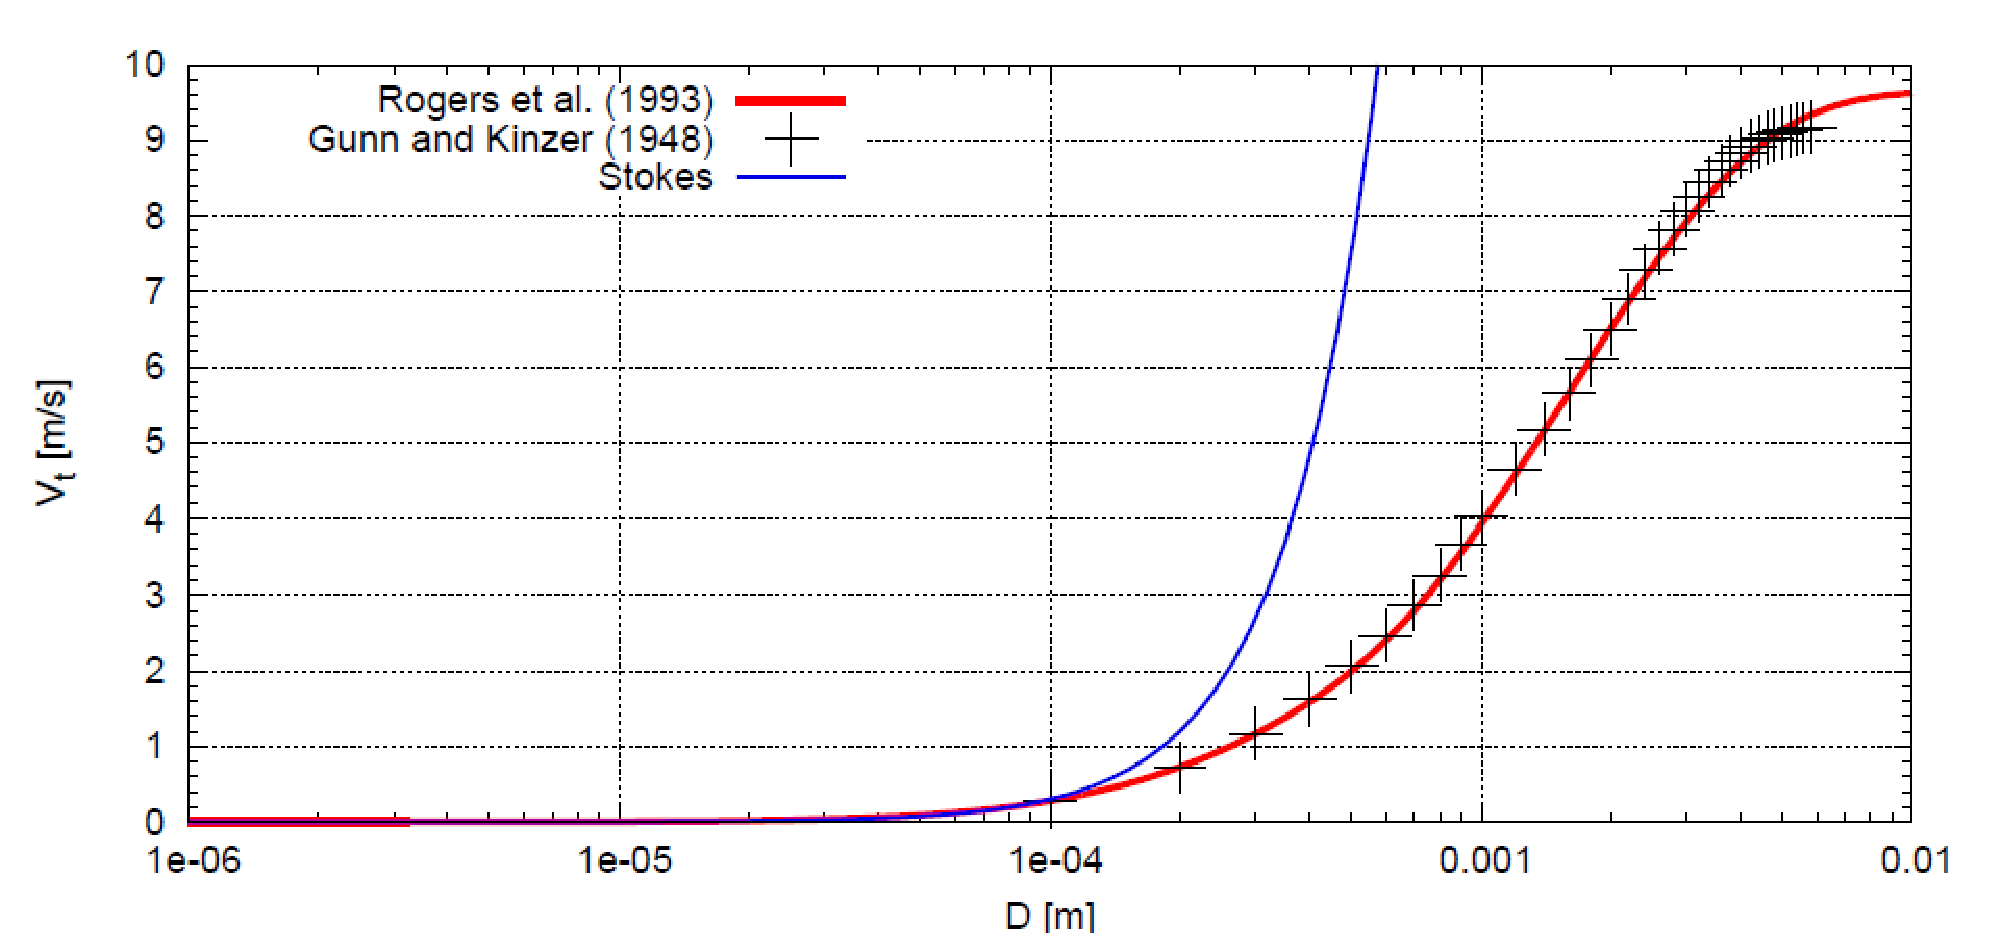
\includegraphics[scale=0.3]{./figure/D_vt_sn14.eps}
\end{center}
\caption{Dependency of terminal velocity of liquid water droplet on diameter. Marks are from Gunn and Kinzer (1948), red line is from Rogers et al. (1993), and blue line is calculated by Stokes’ law (eq.\ref{sn12}) under the condition T=293K, p=1000hPa.}
\label{figsn2-11}
\end{figure}

\begin{figure}[htbp]
\begin{center}
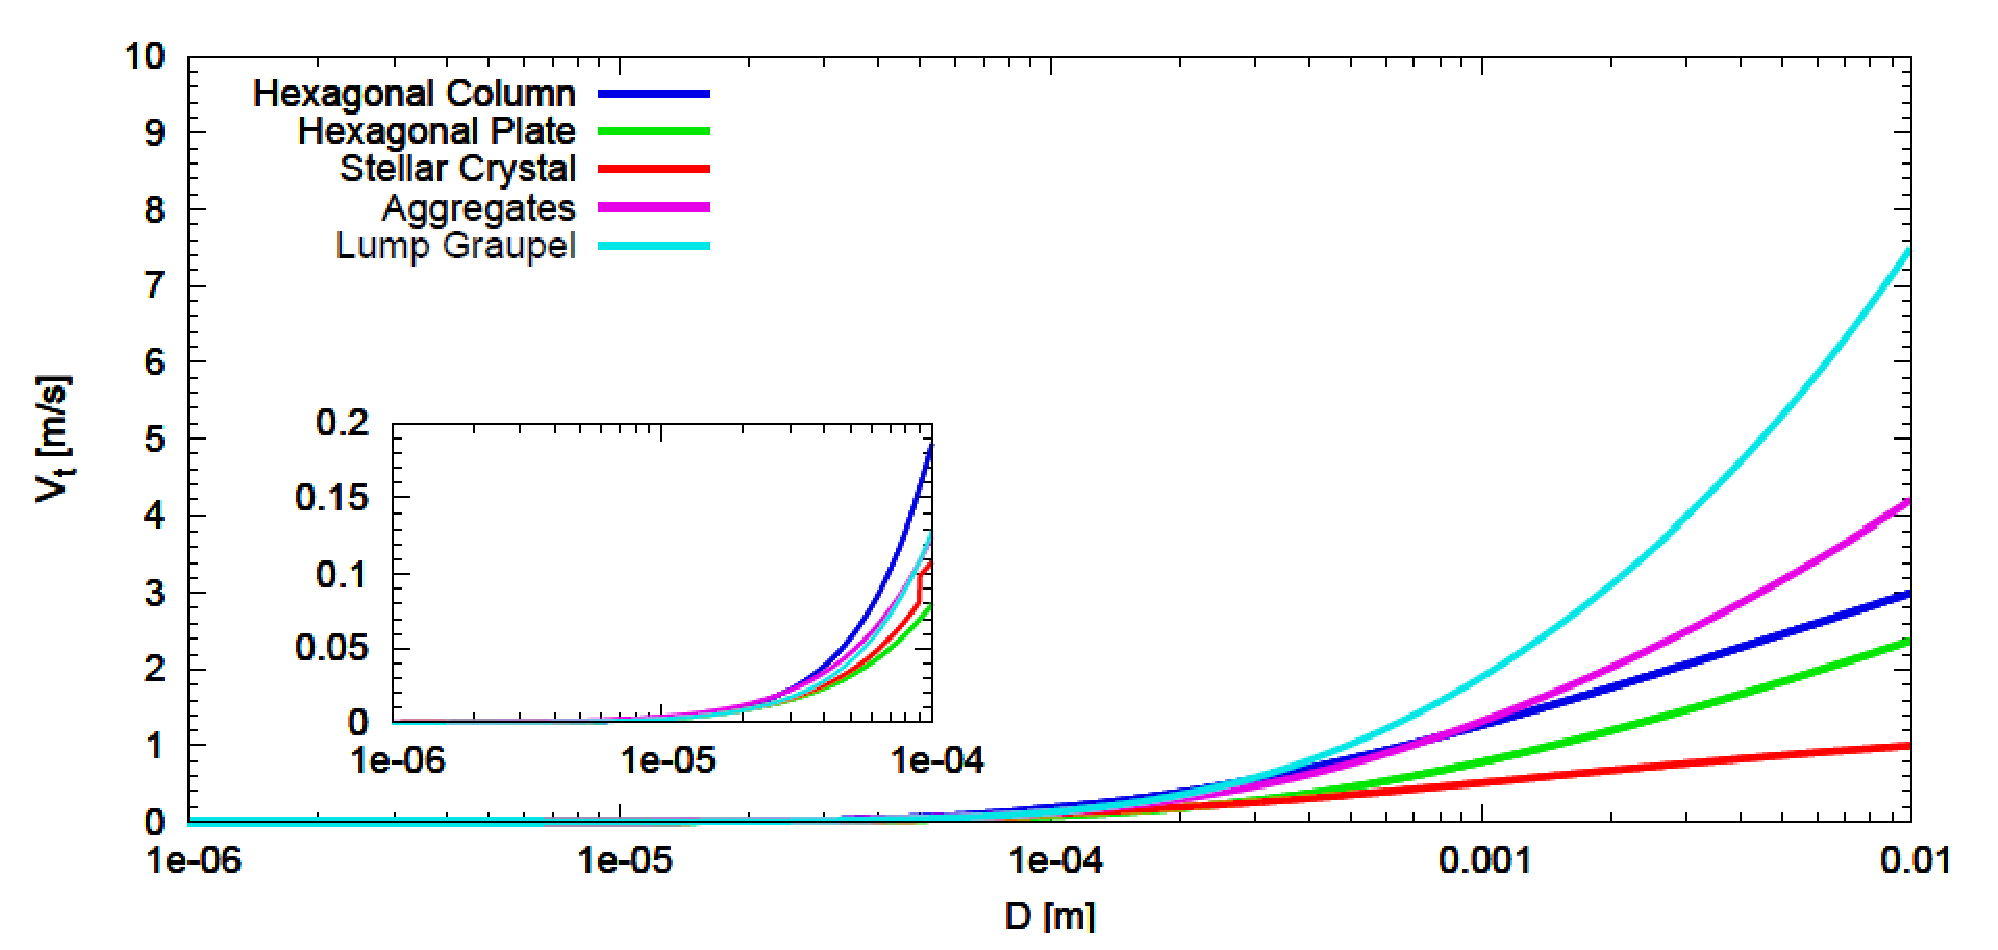
\includegraphics[scale=0.3]{./figure/D_vt_sn14-ice.eps}
\end{center}
\caption{Dependency of terminal velocity of liquid water droplet in maximum dimension. Each solid line color corresponds to different ice particle types, based on Mitchell (1996). Hexagonal columns are blue, hexagonal plates are green, stellar crystals with broad arms are red, aggregates of planar polycrystals in cirrus clouds are purple, and lump graupel is light blue.}
\label{figsn2-12}
\end{figure}

\begin{figure}[htbp]
\begin{center}
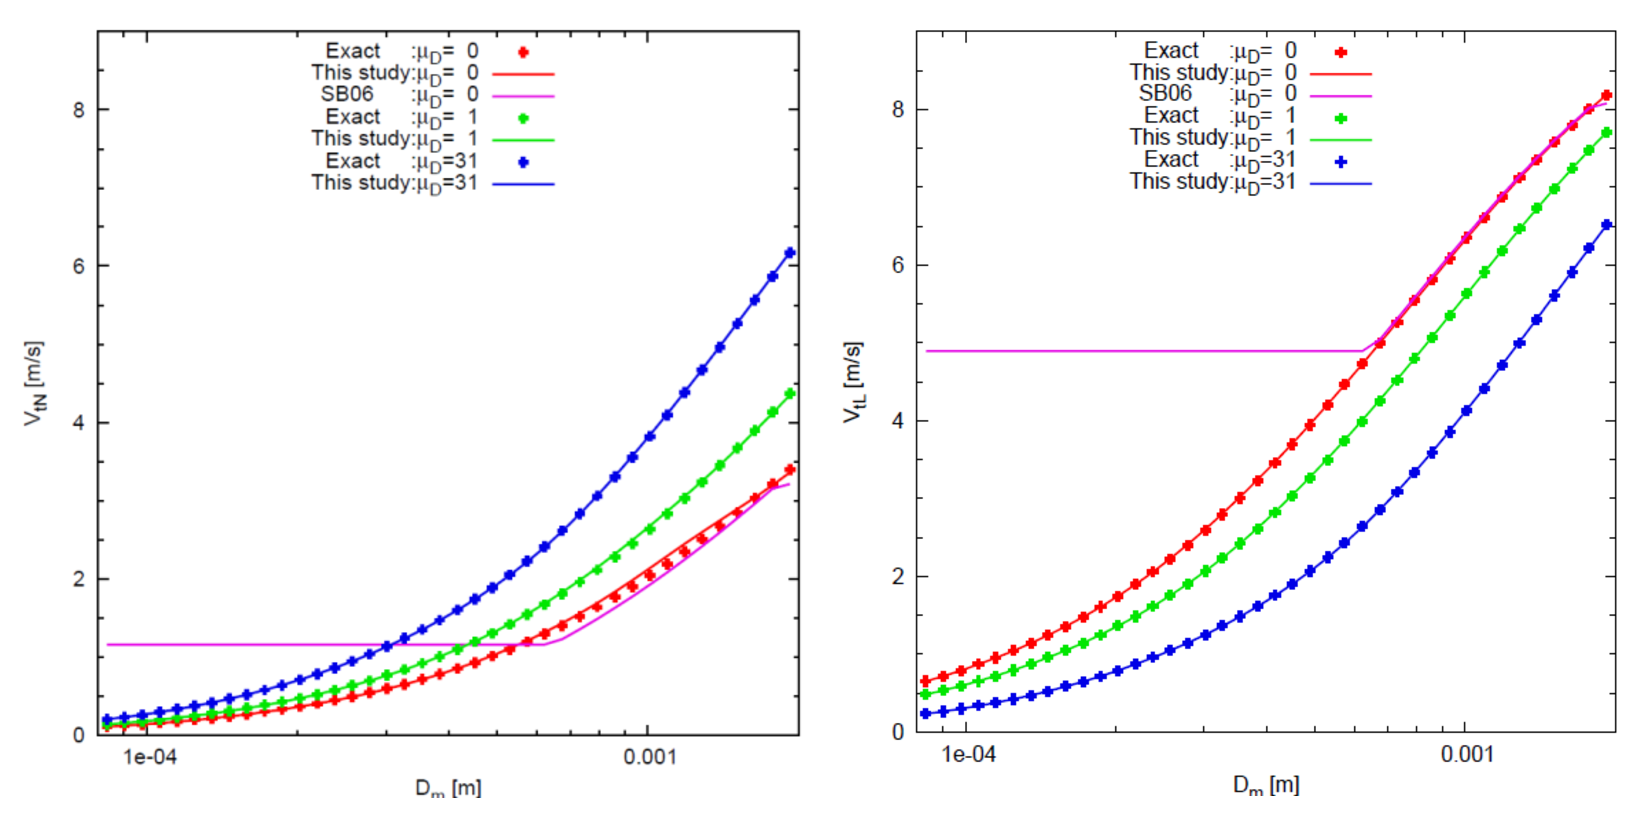
\includegraphics[scale=0.4]{./figure/D_vt_sn14-1.eps}
\end{center}
\caption{Dependencies of number weighted terminal velocity ($v_{tN}$) (left) and mass weighted terminal velocity ($v_{tL}$) (right) of rain droplets on mean volume diameter ($D_{m}$). Abscissa is the mean volume diameter and vertical axis is the terminal velocity. Dots show exactly integrated values and solid lines show approximated values obtained in this study (red, green, and blue) and by Seifert and Beheng (2006) (purple). Red and purple lines are calculated with $\mu D$ = 0, green lines are calculated with $\mu D$ = 1, and blue lines are calculated with $\mu D$ = 31.}
\label{figsn2-13}
\end{figure}

\begin{figure}[htbp]
\begin{center}
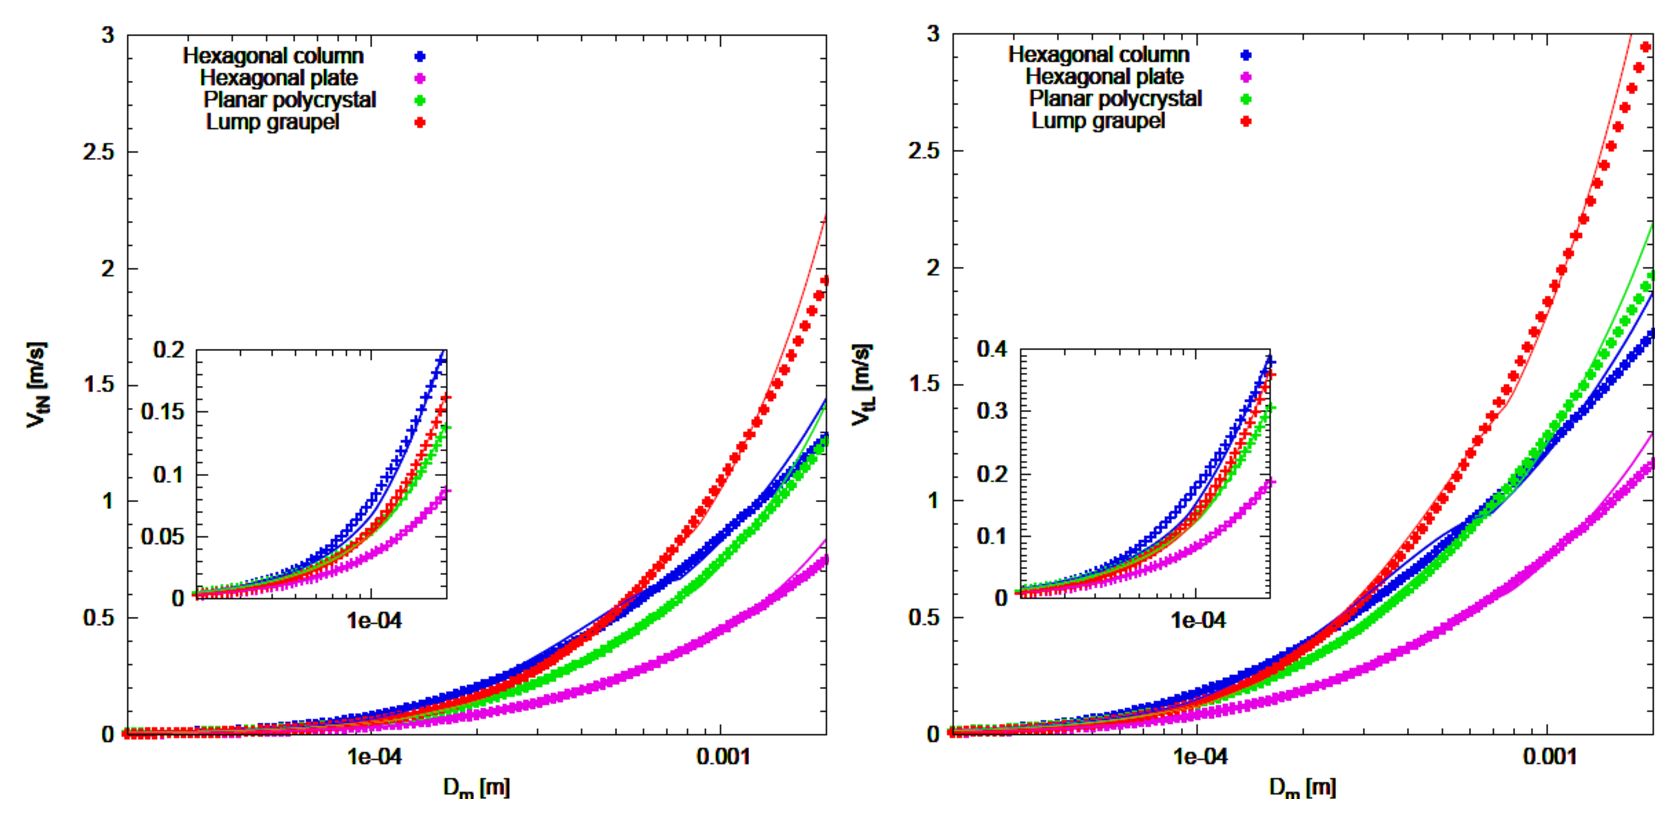
\includegraphics[scale=0.4]{./figure/D_vt_sn14-ice-1.eps}
\end{center}
\caption{Dependencies of number weighted terminal velocity ($v_{tN}$) (left) and mass weighted terminal velocity ($v_{tL}$) (right) of ice particles on mean volume diameter ($D_{m}$). Abscissa is the mean volume diameter and vertical axis is the terminal velocity. Dots show the exact value calculated by Mitchell (1996) and solid lines show the fitting curves. Red, green, blue, and purple denote lump graupels, assemblages of planar polycrystals, hexagonal columns, and hexagonal plates, respectively.}
\label{figsn2-14}
\end{figure}

\subsubsection{Detailed description of cloud microphysics}
Cloud microphysics is mainly subdivided into two. One is phase change among gas, liquid, and solid phases, while the other is the collection process among all particles. In addition, all hydrometeors are vertically transported by gravitational sedimentation. Phase change depends on the thermodynamics of environment air and itself affects thermodynamics through latent heat release. In contrast, collection is an internal growth process with less interaction with the atmosphere. Since the growth speed of the collection process is much faster than that of phase change, the role of the collection process is key to determining the lifetime of clouds (e.g., lifetime effect). Finally, gravitational sedimentation determines the removal rate of clouds from the atmosphere. It removes cloud directly by transportation, and indirectly by the collection process via collision volume (swept volume).\\
The cloud microphysics scheme developed in this study basically follows Seifert and Beheng (2006). Their two-moment bulk cloud microphysics scheme is remarkable in improvement of the collection process by using a bin cloud microphysics scheme. Based on their work, we modify the cloud nucleation process (Twomey 1959; and Lohmann 2002), the condensation process (Morrison et al. 2005), and the formulation of terminal velocities (Mitchell, 1996) with expectation of the application to global cloud resolving simulations. We describe production and reduction terms of mass concentration and number concentration in the following sub-sections.

\subsubsection{Phase change}
\subsubsection{Condensation/evaporation}
Theoretical formulation of condensation or evaporation is basically derived by balance equation of vapor and thermal diffusion above the surface of a single particle (Rogers and Yau, 1989; Pruppacher and Klett, 1997). The growth rate of liquid droplet mass $x_{i}$l is described as follows:

\begin{eqnarray}
\frac{dx_{jl}}{d}&=&2\pi D(x_{jl})G_{lv}(T,p)F_{vf}(x_(jl))S_{w},\; (jl=c,r)\label{sn66}\\
G_{lv}&=&\Bigl[\frac{R_{v}T}{p_{sw}(T)D_{v}}+\frac{L_{v0}}{K_{T}T}\bigl(\frac{L_{v0}}{R_{v}}{T}-1\bigr)\Bigr]^{-1}\label{sn67}\\
F_{vf}(x_{r})&=&a_{vf,r}+b_{vf,r}N_{S_{c}}^{1/3}N_{R_{e}}^{1/2}\label{sn68}
\end{eqnarray}

Here $G_{lv}$ is a coefficient related to vapor and thermal diffusion, $D_{v}$ is diffusivity of water vapor and $K_{T}$ is thermal conductivity, and $F_{vf}$ is the so-called ventilation coefficient. This is a correction factor for the assumption that the water vapor field surrounding each droplet is spherically symmetrical. Formulation of Fvf was experimentally determined by Pruppacher and Klett (1997) and it depends on the Schmidt ($N_{S_{c}}$) and Reynolds ($N_{R_{e}}$) numbers. This formulation for single droplets is transformed into one for moments following Seifert and Beheng (2006). Assuming DSD as a generalized Gamma distribution and neglecting change in DSD caused by other processes in a time step, we can derive the growth rate of moments:

\begin{eqnarray}
\frac{\partial M_{jl}^{k}}{\partial t}\Bigr|_{cnd,evp}\cong \int_{0}^{\infty}f_{jl}(x)x^{k-1}\frac{\partial x}{\partial t}\Bigr|_{cnd,evp}dx\label{sn69}
\end{eqnarray}

We can consider eq.\ref{sn69} from a different view point, as follows:

\begin{eqnarray}
\frac{\partial M_{jl}^{k}}{\partial t}\Bigr|_{cnd,evp}&\cong& \int_{0}^{\infty}f_{jl}(x)x^{k}\Bigl[\frac{1}{x}\frac{\partial x}{\partial t}\Bigr|_{cnd,evp}\Bigr]dx\nonumber\\
&=&\int_{0}^{\infty}\frac{f_{jl}(x)x^{k}}{\tau}dx,\;\tau\equiv\frac{x}{\frac{\partial x}{\partial t}}\bigr|_{cnd,evp}\label{sn70}
\end{eqnarray}

Here, we note that theoretical treatment of condensation or evaporation only changes droplet mass. We then diagnose the growth rates of other moments using the change ratio of droplet mass with time scale $\tau$. We can thus derive the growth equation for arbitrary moments, as follows:

\begin{eqnarray}
\frac{\partial M_{jl}^{k}}{\partial t}\Bigr|_{cnd,evp}&=&2\pi G_{lv}S_{w}\int_{0}^{\infty}D_{jl}(x)F_{vf,jl}(x)f_{jl}(x)x^{k-1}dx\nonumber\\
&=&2\pi G_{lv}S_{w}N_{jl}D_{jl}(\bar{x}_{jl})\bar{F}_{vf,k,jl}(\bar{x}_{jl})\bar{x}_{jl}^{k-1}\label{sn71}
\end{eqnarray}

where $\bar{F}_{vf,k,il}$ is an averaged ventilation factor for the k-th moment of DSD. This formulation seems to be valid unless reduction of number concentration occurs. Because reduction of number concentration occurs only in the case of the smallest droplet being completely dissipated by evaporation, the formulation by change ratio is not suitable for complete dissipation. This formulation is therefore incomplete to derive the reduction tendency of number concentration by evaporation (condensation never changes number concentration). Temporarily, we assumed that the number concentration of cloud droplets never declines unless the mean mass of cloud ($\bar{x}_{c}$) falls below the lower limit $\bar{x}_{c,min}$. The treatment of rain droplets is discussed in the following section.


\subsubsection{Evaporation of rain droplets}
Only in the case of rain droplets, Seifert (2008) attempted to overcome incompleteness for the reduction of number concentration in evaporation. He reformulated eq.\ref{sn71} as follows:

\begin{eqnarray}
\frac{\partial N_{r}}{\partial t}\Bigr|_{evp}\equiv \gamma_{evp}\frac{N_{r}}{L_{r}}\frac{\partial L_{r}}{\partial t}=\frac{\gamma_{evp}}{\bar{x}}2\pi G_{lv}S_{w}N_{r}D_{r}(\bar{x}_{r})\bar{F}_{vf,l}(\bar{x}_{r})\label{sn72}
\end{eqnarray}

Here, evaporation parameter $\gamma_{evp}$ means the evaporation efficiency of number concentration towards mean mass $\bar{x}_{r}$. According to Seifert (2008), $\gamma_{evp}$ and $\mu_{m,r}$ are parameterized as follows:

\begin{eqnarray}
\gamma_{evp}&=&\frac{D_{eq}}{D(\bar{x}_{r})}exp(-0.2\mu_{m,r})\label{sn73}\\
\mu_{m,r}&=&
\left\{
\begin{array}{l}
6tauh[{c_{evp,1}(D(\bar{x}_{r})-D_{eq})}^{2}]+1\;\;(D(\bar{x}_{r})\leq D_{eq}) \\
30tauh[{c_{evp,2}(D(\bar{x}_{r})-D_{eq})}^{2}]+1\;\;(D(\bar{x}_{r})\leq D_{eq})
\label{sn74}
\end{array}
\right.
\end{eqnarray}

where $D_{eq} = 1.1 \times 10^{-3} m$ is the equilibrium diameter in breakup-coalescence processes, and $c_{evp,1}$ and $c_{evp,2}$ are set to 4000 $m^{-1}$ and 1000 $m^{-1}$, respectively. In this study, we apply eq.\ref{sn71} for mass and eq.\ref{sn72} with $\gamma_{evp}$ = 1 for number concentration as a default setting (refer to SB06-run).

\subsubsection{Deposition/sublimation for solid water}
Theoretical formulation of deposition or sublimation is the same as that of condensation or evaporation, except for the definition of surface area. The shape of ice particles is not spherical and varies widely, as shown in section 2.1.2. Vapor and thermal transfer over the particle surface are therefore expressed by the analogy between the diffusion equation and equations in electrostatics (Pruppacher and Klett, 1997). Replacing diameter $D_{js}$ by capacitance $C_{js}\equiv D{js}/c_{js}$, we can derive the growth equation of a single particle, as follows:

\begin{eqnarray}
\frac{dx_{js}}{dt}\Bigr|_{dep,sbl}&=&4\pi C_{js}G_{sv}(T,p)F_{vf}(x_{js})S_{i},\;\;(js=i,s,g)\label{sn75}\\
G_{sv}&=&\Bigl[\frac{R_{v}T}{p_{si}(T)D_{v}}+\frac{L_{s,0}}{K_{T}T}\bigl(\frac{L_{s0}}{R_{v}T}-1\bigr)\Bigr]^{-1}\label{sn76}
\end{eqnarray}

Here $C_{js}$ = $D_{js}/2$ for sphere, $C_{js} = D_{js}/\pi$ for circular plate, and capacitance of other typical shapes (such as oblate spheroid crystals and columnar crystals) are expressed by:

\begin{eqnarray}
C_{js}&=&\frac{D_{js}\varepsilon}{2sin^{-1}\varepsilon},\;\;\varepsilon\equiv\bigl(1-\frac{b^{2}}{a^{2}}\bigr), \;(for\;spheroid)\label{sn77}\\
C_{js}&=&\frac{A}{ln[(a+A)/b]},\;A\equiv=(a^{2}-b^{2})^{1/2},\;\;(for\;columnar)
\end{eqnarray}

where a is the semi-major axis and b is the semi-minor axis. For simplification, cloud, rain, snow, and graupel are assumed to be spherical, and hexagonal plate ice is assumed to be a circular plate. In the same manner as condensation (evaporation), we can derive the growth equation of arbitrary moments, as follows:

\begin{eqnarray}
\frac{\partial M_{js}^{k}}{\partial t}\Bigr|_{dep,sbl}=\frac{4\pi}{c_{js}}G_{sv}S_{i}N_{js}D_{js}(\bar{x}_{js})\bar{F}_{vf,k}(\bar{x}_{js})\bar{x}_{js}^{k-1}\label{sn79}
\end{eqnarray}

The discussion concerning the reduction term of number concentration is the same as for rain droplets. We therefore applied eq.\ref{sn79} for mass concentration of solid particles. For snow and graupel, the reduction rate of number concentration is as follows:

\begin{eqnarray}
\frac{\partial N_{js}^{k}}{\partial t}\Bigr|_{sbl}&\equiv&\frac{N_{js}}{L_{js}}\frac{\partial L_{js}}{\partial t}\Bigr|_{sbl}\nonumber\\
&=&\frac{1}{\bar{x}_{js}}\frac{4\pi}{c_{js}}G_{sv}S_{i}N_{js}D_{js}(\bar{x}_{js})\bar{F}_{vf,1}(\bar{x}_{js})(js=s,g)\label{sn80}
\end{eqnarray}

This formulation corresponds to $\gamma_{evp} = 1$ in the reduction term for rain droplets. This means that sublimation occurs so as not to change the mean mass of DSD ($\bar{x}_{js}$). Number concentration of ice never reduces in sublimation unless the mean mass of ice ($\bar{x}_{i}$) falls below the lower limit. The formulations of the reduction rate for the number concentration of ice particles are somewhat temporary and will be improved based on insights drawn from the results of microphysics bin schemes and observations in future.

\subsubsection{Accurate integration method to solve condensation/evaporation and deposition/sublimation}
The condensation/evaporation process for cloud droplets usually requires a smaller time step than rain droplets or other particles because of its timescale. When we apply time integration with the first-ordered Euler method, the accuracies of condensation/evaporation and deposition/sublimation processes are poor unless we resolve their timescale. We initially estimate the timescale with the exact thermodynamic definition in NICAM and then formulate an accurate method to apply the condensation and evaporation processes for cloud droplets, similar to Khvorostyanov and Sassen (1998) and Morrison et al., (2005). Since the supersaturated condition is achieved by updraft of air mass, we consider a Lagrangian parcel model with constant updraft velocity and no mixing with external air mass. Basic formulation is based on the Lagrangian change rate of supersaturation ($\delta_{sw} = q_{v} - q_{sw}$), as follows:

\begin{eqnarray}
\frac{d \delta_{sw}}{dt}=\Bigl(\frac{dq_{v}}{dt}-\frac{dq_{sw}}{dt}\Bigr)\label{sn81}
\end{eqnarray}

Hereafter, we consider the tendency of specific humidity and saturation, specific humidity by dynamics, cloud microphysics, and radiative heating.\\
At first, assuming an adiabatically ascending/descending parcel with no phase change ($q_{v}/dt = 0$), eq.(\ref{sn81}) becomes:

\begin{eqnarray}
\frac{d\delta_{sw}}{dt}=-\bigl(\frac{\partial q_{sw}}{\partial T}\bigr)_{p}\frac{dT}{dt}-\bigl(\frac{\partial q_{sw}}{\partial p}\bigr)_{T}\frac{dp}{dt}\label{sn82}
\end{eqnarray}

Here, the tendencies of temperature and pressure are described as follows:

\begin{eqnarray}
\frac{dT}{dt}=\frac{1}{\rho\bar{c}_{p}}\frac{dp}{dt},\;\;\frac{dp}{dt}\approx-\rho g w\label{sn83}
\end{eqnarray}

where $\bar{c}_{p}\equiv q_{d}c_{pd}+q_{v}c_{pv}+q_{liq}c_{l}+q_{sol}c_{i}$ is the mean specific heat at constant pressure. We can derive the dynamic component of the tendency of $\delta_{sw}$ by substituting eq. \ref{sn83} into eq.\ref{sn82}, as follows:

\begin{eqnarray}
\frac{d\delta_{sw}}{dt}\Bigr|_{DYN}=wg\Bigl(\frac{1}{\bar{c}_{p}}\bigl(\frac{\partial q_{sw}}{\partial T}\bigr)_{p}+\rho\bigl(\frac{\partial q_{sw}}{\partial p}\bigr)_{T}\Bigr)\label{sn84}
\end{eqnarray}

Assuming an air parcel with only cooling/heating by latent heat release, eq. \ref{sn81} becomes:

\begin{eqnarray}
\frac{d\delta_{sw}}{dt}=\frac{dq_{v}}{dt}-\bigl(\frac{\partial q_{sw}}{\partial T}\bigr)\frac{dT}{dt}\label{sn85}
\end{eqnarray}

The tendency of temperature is caused by latent heat release with condensation/evaporation and deposition/sublimation:  %eq.\ref{sn58}, eq.\ref{sn59} %, and Table \ref{table_sn14-2-11}:

\begin{eqnarray}
\frac{dT}{dt}&=&\frac{L_{v,00}+(c_{vv}-c_{l})T}{\bar{c}_{va}}\frac{dq_{liq}}{dt}+\frac{L_{v,00}+L_{f,00}+(c_{v}-c_{i})T}{\bar{c}_{va}}\frac{dq_{sol}}{dt}\nonumber\\
&=&\frac{L_{v,00}+(c_{vv}-c_{l}) T}{\bar{c}_{va}} \sum^{jl_{max}}_{jl=1}\frac{dq_{jl}}{dt}\Bigr|_{cnd,evp}\nonumber\\
&+&\frac{L_{v,00}+L_{f,00}+(c_{vv}-c_{i})T}{\bar{c}_{va}}\sum^{js_{max}}_{js=1}\frac{dq_{js}}{dt}\Bigr|_{dep,sbl}\label{sn86}
\end{eqnarray}

The tendency of specific humidity is caused by condensation/evaporation and deposition/sublimation:

\begin{eqnarray}
\frac{dq_{v}}{dt}=-\sum_{jl=1}^{jl_{max}}\frac{dq_{jl}}{dt}\Bigl|_{cnd,evp}-\sum_{js=1}^{js_{max}}\frac{dq_{js}}{dt}\Bigr|_{dep,sbl}\label{sn87}
\end{eqnarray}

We can then derive the cloud microphysics component of the tendency of $\delta_{sw}$ by substituting eqs.\ref{sn86} and \ref{sn87} into eq.\ref{sn85}:

\begin{eqnarray}
\frac{d\delta_{sw}}{dt}\Bigr|_{MP}&=&-\Bigl(1+\frac{L_{v,00}+(c_{vv}-c_{l})T}{\bar{c}_{v}}\bigl(\frac{\partial q_{sw}}{\partial T}\bigr)_{p}\Bigr)\sum_{jl=1}^{jl_{max}}\partial{dq_{jl}}{dt}\Bigr|_{cnd,evp}\nonumber\\
&-&\Bigl(1+\frac{L_{v,00}+L_{f,00}+(c_{vv}-c_{i})T}{\bar{c}_{v}}\bigl(\frac{\partial q_{sw}}{\partial T}\bigr)_{p}\Bigr)\sum^{js_{max}}_{js=1}\frac{dq_{js}}{dt}\Bigr|_{dep,sbl}\label{sn88}
\end{eqnarray}

By replacing the source term of the mixing ratio of hydrometeors in eq.\ref{sn88} with eqs.\ref{sn71} and \ref{sn79}:

\begin{eqnarray}
\frac{dq_{jl}}{dt}\Bigr|_{cnd,evp}&=&\frac{\delta_{sw}}{\tau_{cnd,jl}},\;or\nonumber\\
\frac{dq_{jl}}{dt}\Bigr|_{cnd,evp}&=&\frac{\delta_{si}}{\tau_{cnd,jl}}-\frac{q_{sw}-q_{si}}{\tau_{cnd,jl}},\;\;(jl=c,r)\label{89}\\
\frac{dq_{js}}{dt}\Bigr|_{de,sbl}&=&\frac{\delta_{si}}{\tau_{dep,js}},\;or\nonumber\\
\frac{dq_{js}}{dt}\Bigr|_{dep,sbl}&=&\frac{\delta_{sw}}{\tau_{dep,js}}+\frac{q_{sw}-q_{si}}{\tau_{dep,js}},\;\;(js=i,s,g)\label{90}\\
\tau_{cnd,jl} &\equiv& \Bigl(\frac{1}{\rho q_{sw}} 2\pi G_{lv}D_{jl}(\bar{x}_{jl})N_{jl}\bar{F}_{vf,1}\Bigr)^{-1}\label{sn91}\\
\tau_{dep,js} &\equiv& \Bigl(\frac{1}{\rho q_{si}}\frac{4\pi}{c_{js}}G_{sv}D_{js}(\bar{x}_{js})N_{js}\bar{F}_{vf,1}\Bigr)^{-1}\label{sn92}
\end{eqnarray}


We can rewrite eq.\ref{sn88} as a function of super saturation itself:

\begin{eqnarray}
\frac{\partial \delta_{sw}}{\partial t}\Bigr|_{MP}=&-&\bigl(\frac{a_{liq,liq}}{\tau_{cnd,c}}+\frac{a_{liq,liq}}{\tau_{cnd,r}}+\frac{a_{sol,liq}}{\tau_{dep}}+\frac{a_{sol,liq}}{\tau_{dep,s}}+\frac{a_{sol,liq}}{\tau_{dep,g}}\bigr)\delta_{sw}\nonumber\\
&-&\bigl(\frac{1}{\tau_{dep,i}}+\frac{1}{\tau_{dep,s}}+\frac{1}{\tau_{dep,g}}\bigr)(q_{sw}-q_{si})\label{sn93}\\
a_{liq,liq}&\equiv& 1+\frac{L_{v00}+(c_{vv}-c_{l})T}{\bar{c}_{v}}\bigl(\frac{\partial q_{sw}}{\partial T}\bigr)_{p}\label{94}\\
a_{sol,liq}&\equiv& 1+\frac{L_{v00}+L_{f00}+(c_{vv}-c_{i})T}{\bar{c}_{v}}\bigl(\frac{\partial q_{sw}}{\partial T}\bigr)_{p}\label{95}
\end{eqnarray}

Here, we can find that $\tau_{cnd,jl}$ and $\tau_{dep,js}$ in eq.\ref{sn93} are considered as the characteristic time scale for relaxation of the super saturation condition by condensation/evaporation and deposition/sublimation processes. The timescale of each hydrometeor is modified by coefficient $a_{liq,liq}$ or $a_{sol,liq}$, indicating the effect of latent heat release. The second term on the right hand side in eq.\ref{sn93} means the transfer of vapor from liquid droplets to solid particles. The Bergeron-Findeisen process is implicitly formulated by the difference of saturation vapor pressure between liquid and solid.\\
Finally, assuming an air parcel with radiative heating (cooling), eq.\ref{sn81} becomes

\begin{eqnarray}
\frac{d\delta_{sw}}{dt}\Bigr|_{RAD}=-\bigl(\frac{\partial q_{sw}}{\partial T}\bigr)_{\rho}\bigl(\frac{dT}{dt}\bigr)_{RAD}\label{sn96}
\end{eqnarray}

All the components in the Lagrangian ascending/descending parcel model are described by eqs.\ref{sn84}, \ref{sn93}, and \ref{sn96}:

\begin{eqnarray}
\frac{d\delta_{sw}}{dt}&=&A_{cnd}-\frac{\delta_{sw}}{\tau_{cnd}}\label{sn97}\\
A_{cnd}&\equiv&\frac{d\delta_{sw}}{dt}\Bigr|_{DYN}+\frac{d\delta_{sw}}{dt}\Bigr|_{RAD}\nonumber\\
&-&\bigl(\frac{1}{\tau_{dep,i}}+\frac{1}{\tau_{dep,s}}+\frac{1}{\tau_{dep,g}}\bigr)(q_{sw}-q_{si})\label{sn98}\\
\tau_{cnd}&\equiv&\bigl(\frac{a_{liq,liq}}{\tau_{cnd,c}}+\frac{a_{liq,liq}}{\tau_{cnd,r}}+\frac{a_{sol,liq}}{\tau_{dep,i}}+\frac{a_{sol,liq}}{\tau_{dep,s}}+\frac{a_{sol,liq}}{\tau_{dep,g}}\bigr)^{-1}\label{sn99}
\end{eqnarray}

Here, we can see that $A_{cnd}$ is a production term of super saturation and τcnd is a characteristic timescale of all phase changes. From formulations of eqs.\ref{sn91} and \ref{sn92}), we find that the timescale of each hydrometeor is in inverse proportion to its number concentration. Therefore, the timescale of cloud droplets is the shortest one in all hydrometeors because the typical numbers of cloud droplets are about 10,000 times more than any others. The timescales under various conditions are shown in Fig.\ref{figsn2-19}.\\
Assuming that time variance of the production term and the timescale in a simulation time step do not vary much within a model timestep, we can analytically solve eq.\ref{sn97}:

\begin{eqnarray}
\delta_{sw}(t)=A_{cnd}\tau_{cnd}+(\delta_{sw}(t_{0})-A_{cnd}\tau_{cnd})exp\bigl(-\frac{t}{\tau_{cnd}}\bigr)\label{sn100}
\end{eqnarray}

where $t = t_{0} + \Delta t$ and $t_{0} = 0$. Then, the condensation (evaporation) rates of cloud and rain are reformulated by substituting eq.\ref{sn100} into eq.\ref{sn71} and integrating these:

\begin{eqnarray}
\frac{\Delta L_{jl}}{\Delta t}\Bigr|_{cnd,evp}&=&\rho A_{cnd}\frac{\tau_{cnd}}{\tau_{cnd,jl}}\nonumber\\
&-&\rho\frac{(\delta_{sw}(t_{0})-A_{cnd}\tau_{cnd})}{\Delta t}\frac{\tau_{cnd}}{\tau_{cnd,jl}}\Bigl[exp\bigl(-\frac{\Delta t}{\tau_{cnd}}\bigr)-1\Bigr]\label{sn101}
\end{eqnarray}

This semi-analytical formulation takes time variability of super saturation into condensation (evaporation) growth. It is therefore better than direct time integration with a first-order Euler method.\\
In the same manner, we can also derive the semi-analytical formulation for deposition (sublimation) with super saturation for solid water: ($\delta_{si}$),

\begin{eqnarray}
\delta_{si}(t)&=&A_{dep}\tau_{dep}+(\delta_{si}(t_{0})-A_{dep}\tau_{dep})exp\bigl(-\frac{t}{\tau_{dep}}\bigr)\label{sn103}\\
\frac{\Delta L_{js}}{\Delta t}\Bigr|_{dep,sbl}&=&\rho A_{dep}\frac{\tau_{dep}}{\tau_{dep,js}}\nonumber\\
&-&\rho\frac{(\delta_{si}(t_{0})-A_{dep}\tau_{dep})}{\Delta t}\frac{\tau_{dep}}{\tau_{dep,js}}\Bigl[exp\bigl(-\frac{\Delta t}{\tau_{dep}}\bigr)-1\Bigr]\label{sn104}
\end{eqnarray}

where:

\begin{eqnarray}
A_{dep}&\equiv&\frac{d\delta_{si}}{dt}\Bigr|_{DYN}+\frac{d\delta_{si}}{dt}\Bigr|_{RAD}\nonumber\\
&+&\bigl(\frac{1}{\tau_{cnd,c}}+\frac{1}{\tau_{cnd,r}}\bigr)(q_{sw}-q_{si})\label{sn105}\\
\tau_{dep}&\equiv&\bigl(\frac{a_{liq,sol}}{\tau_{cnd,c}}+\frac{a_{liq,sol}}{\tau_{cnd,r}}+\frac{a_{sol,sol}}{\tau_{dep,i}}+\frac{a_{sol,sol}}{\tau_{dep,s}}+\frac{a_{sol,sol}}{\tau_{dep,g}}\bigr)^{-1}\label{sn106}\\
a_{liq,sol}&\equiv&1+\frac{L_{v00}+(c_{vv}-c_{l})T}{\bar{c}_{v}}\bigl(\frac{\partial q_{si}}{\partial T}\bigr)_{p}\nonumber\\
a_{sol,sol}&\equiv&1+\frac{L_{v00}+L_{f00}+(c_{vv}-c_{i})T}{\bar{c}_{v}}\bigl(\frac{\partial q_{si}}{\partial T}\bigr)_{p}\nonumber\\
\frac{d\delta_{si}}{dt}\Bigr|_{DYN}&=&wg\Bigl(\frac{1}{\bar{c}_{p}}\bigl(\frac{\partial q_{si}}{\partial T}\bigr)_{p}+\rho\bigl(\frac{\partial q_{si}}{\partial p}\bigr)_{T}\Bigr)\nonumber\\
\frac{d\delta_{si}}{dt}\Bigl|_{RAD}&=&-\bigl(\frac{\partial q_{si}}{\partial T}\bigr)_{\rho}\bigl(\frac{dT}{dt}\bigr)_{RAD}\nonumber
\end{eqnarray}

Finally, we applied eqs.\ref{sn101} and \ref{sn104} for prediction of mass concentration and eqs.\ref{sn72} and \ref{sn80} for prediction of number concentrations of rain, snow, and graupel. Number concentrations of cloud and ice are assumed not to change by evaporation and sublimation.


\subsubsection{Nucleation of cloud droplets}
Seifert and Beheng (2006) applied a traditional empirical formulation as an aerosol activation spectrum, as follows:

\begin{eqnarray}
N_{c}(S_{w,100})=C_{ccn}S_{w,100}^{\kappa_{ccn}}\label{sn107}
\end{eqnarray}

where the super saturation ratio $S_{w,100}$ is in %. They use $C_{ccn} = 1.26 \times 10^{9} m^{-3}$ and $\kappa_{ccn} = 0.308$ in continental conditions and $C_{ccn} = 1.0 \times 10^{8} m^{-3}$ and $\kappa_{ccn} = 0.462$ in maritime conditions. Further, Seifert and Beheng (2006) transformed eq.\ref{sn107} into a tendency formulation by time differentiation of the activation spectrum:

\begin{eqnarray}
\frac{\partial N_{c}}{\partial t}&=&
\left\{
\begin{array}{l}
C_{ccn}\kappa_{ccn}S_{w,100}^{\kappa_{ccn}-1}\frac{\partial S_{w,100}}{\partial z}w\nonumber\\
(S_{w,100}>0,\;w\frac{\partial S_{w,100}}{\partial z}>0,\;and\;S_{w,100}<1.1) \nonumber\\
0,\;\;(else)
\end{array}
\right.\\
\label{sn108}
\frac{\partial L_{c}}{\partial t}\Bigr|_{nuc}&=&x_{c,nuc}\frac{\partial N_{c}}{\partial t}\Bigr|_{nuc}\label{sn109}
\end{eqnarray}

where $x_{c,nuc} = 10^{-12} kg$ is an arbitrary mass of nucleated droplets. Because the aerosol activity spectrum is a function of supersaturation and is unbounded by total aerosol number concentration, we chose an upper limit of activated aerosols as $1.5 \times C_{ccn}$, as similarly chosen by SB06. The maximum activated aerosol number concentration is 1.5 times the activated aerosol number concentration at ssw = 1 $^{o}/_{o}$. It should be noted that this formulation depends on the grid value of super saturation ratio, vertical velocity, and vertical derivation of the super saturation ratio. Since super saturation significantly varies with tens of meters above the cloud base (see Fig.\ref{figsn2-21}), accurate prediction of super saturation and its vertical derivation is quite difficult. In this study, we applied a traditional nucleation scheme (Twomey, 1959; Rogers and Yau, 1989) following Morrison et al. (2005):

\begin{eqnarray}
N_{c,nuc}(w_{eff})&=&0.88C_{ccn}^{2/(\kappa_{ccn}+2)}(0.07w_{eff}^{3/2})^{\kappa_{ccn}/(\kappa_{ccn}+2)}\label{sn110}\\
w_{eff}&\equiv&w+w_{TB}-\frac{\bar{c}_{p}}{g}\bigl(\frac{dT}{dt}\bigr)_{RAD}\label{sn111}
\end{eqnarray}

where $w_{eff}$ is effective vertical velocity for nucleation and $w_{TB}$ is the sub-grid variability of terminal velocity. This is an analytical formulation of maximum number concentration around the cloud base for the Twomey equation, with aerosol activated spectrum by eq.\ref{sn107} (see Fig.\ref{figsn2-18}). Using this scheme, we do not have to resolve the vertical variability of super saturation around the cloud base. Furthermore, applying sub-grid turbulence effects on vertical velocity reduces under-estimation of nucleated cloud number concentration caused by low horizontal resolution (Ghan et al., 1997; Lohmann, 2002; Morrison and Pinto, 2005). In this study, implementation of the sub-grid turbulence effect follows Lohmann (2002):

\begin{eqnarray}
w_{TB}&=&c_{TB}\bigl(\frac{2}{3}TKE\bigr)^{1/2}\label{sn112}\\
\bar{N}_{c,nucl}&=&0.1\times N_{c,nuc}(w_{eff})^{1.27}\label{sn113}
\end{eqnarray}

where $c_{TB} = 1$ is used in this study, $\bar{N}_{c,nuc}$ $cm^{-3}$ is a grid-averaged nucleated cloud number concentration, and $N_{c,nuc}(w_{eff}) cm^{-3}$ is maximum cloud number concentration in turbulent air. By substituting eqs.\ref{sn110}, \ref{sn111}, and \ref{sn112} into eq.\ref{sn113}, the tendency of cloud number concentration is calculated as follows:

\begin{eqnarray}
\frac{\partial N_{c}}{\partial t}\Bigr|_{nucl}&=&
\left\{
\begin{array}{l}
\frac{N_{c,nu}(w_{eff})-N_{c}}{\Delta t},\;\;(S_{w}>0,\;\bar{N}_{c,nuc}>N_{c}\;and\;at\;cloud\;base) \\
0,\;\;(else) \\
\label{sn114}
\end{array}
\right.\\
\frac{\partial L_{c}}{\partial t}\Bigr|_{nuc}&=&min\Bigl(x_{c,min}\frac{\partial N_{c}}{\partial t}\bigr|_{nuc},\frac{\delta_{sw}}{\Delta t}\Bigr)\label{sn115}
\end{eqnarray}

Since nucleation is usually limited around the cloud base within several tens of meters (see Fig.\ref{figsn2-21}), we define the cloud base layer ($k_{cbase}$) where the nucleation scheme works as follows:

\begin{eqnarray}
1.5 \times C_{ccn} > \bar{N}_{c,nu}(k_{cbase})>0,\;\;and\;\;\bar{N}_{c,nu}(k_{cbase}-1) < 10^{6}\label{sn116}
\end{eqnarray}

In addition, we prepare the option (NO-TB) to switch off the effect of turbulence by substituting eqs.\ref{sn110} and \ref{sn111} with $w_{TB} = 0$ into eq.\ref{sn114}. However, there remain some problems to be solved in future:\\
1.Definition of cloud base is empirical and arbitrary.\\
2.Implementation of sub-grid scale is empirical and $c_{TB}$ is a kind of tuning parameter. In particular, the TKE approach only considers isotropic eddies. Sub-grid should be expressed as sub-grid cloud dynamics.\\
3.Formulation of eq.\ref{sn113} does not converge with the NO-TB option when TKE = 0.\\
We need to investigate the above problems by using a large eddy simulation (LES) cloud model.

\subsubsection{Nucleation of cloud ice}
This study employed two simple ice nucleation schemes, which do not require the properties of ice nuclei. One is the depositional and condensational freezing nucleation scheme parameterized by Meyers et al. (1992):

\begin{eqnarray}
N_{IN}=10^{3}exp(-0.639+12.96S_{sol})\nonumber
\end{eqnarray}

where $N_{IN}$ is nucleated ice nuclei and $S_{sol}$ is supersaturation for solid water. While this scheme is widely used in CRMs (e.g., Walko et al. 1995; Khain et al., 2000; Seifert and Beheng, 2006), it is not acceptable for temperature conditions < -20 ˚C or supersaturation > 0.25, where observational data were not available in their study. For simulating cirrus clouds around the tropopause, application of this scheme to CRMs may cause significant error. Phillips et al. (2007) proposed an alternative scheme to modify Meyers’s scheme by fitting observational data at temperatures between -30 ˚C and -80 ˚C obtained by Demott et al. (2003):

\begin{eqnarray}
N_{IN}=10^{3}exp[0.3\times12.96(S_{i}-0.1)]\label{sn117}
\end{eqnarray}

In this study, the nucleation rate is formulated by newly nucleated ice nuclei with supersaturation tendency in the same manner as Murakami (1990):

\begin{eqnarray}
\frac{\Delta N_{i}}{\Delta t}&=&
\left\{
\begin{array}{l}
\frac{\partial N_{IN}}{\partial S_{sol}}\frac{\partial S_{sol}}{\partial t},\;\;(S_{sol}>0\;and\;\frac{\partial S_{sol}}{\partial t}>0) \\
0,\;\;(else) \\
\end{array}
\right.\\
\label{sn118}
\frac{\partial S_{sol}}{\partial t}&\approx& \Bigl[\frac{\partial S_{sol}}{\partial z}w+\bigl(\frac{\partial S_{sol}}{\partial T}\bigr)\bigl(\frac{\partial T}{\partial t}\bigr)_{RAD}\Bigr]\nonumber\\
\frac{\Delta L_{i}}{\Delta t}\Bigr|_{nuc}&=&\frac{\Delta N_{i}}{\Delta t}\Bigr|_{nuc}x_{IN}\label{sn119}
\end{eqnarray}

where $x_{IN} = 10^{-12} kg$ is an arbitrary parameter for a nucleated ice nuclei mass. Here, we assume the change of supersaturation comes from the vertical motion of air masses and radiative cooling. Meyers’s scheme better reflects the number concentration of cloud ice than Phillips’s scheme, and the divergence becomes larger as supersaturation increases. This difference stems from the sampled air masses used in observational data that the schemes referred to and from implicit dependencies of the schemes on temperature and aerosol species. It is expected that Phillips’s scheme is appropriate for simulation of mid-latitude cirrus clouds because it is based on air masses sampled in the free troposphere in mid-latitudes, while Meyers’s scheme is based on air masses sampled in the atmospheric boundary layer, which is rich in ice nuclei.

\subsubsection{Freezing}
The freezing process involves two types of mechanisms. One is homogenous freezing, i.e., freezing of supercooled water droplets without other agents. Another is heterogeneous freezing, i.e., freezing of supercooled water droplets with insoluble parts of aerosols dissolved in cloud droplets. We apply the same parameterizations for both homogeneous and heterogeneous freezing as Seifert and Beheng (2006a). Cotton and Field (2002) parameterized the homogeneous freezing rate for a single droplet by fitting to the theoretical estimation of Jeffery and Austin (1997). We apply their parameterization as per Seifert and Beheng (2006a):

\begin{eqnarray}
\frac{1}{f_{c}(x)}\frac{\partial f_{c}(x)}{\partial t}\Bigr|_{hom}=-xJ_{hom}(T_{c})\label{sn120}
\end{eqnarray}

where $J_{hom}$ is a homogeneous freezing rate ($kg^{-1}s^{-1}$) and $T_{c}$ is centigrade temperature. $J_{hom}$ is formulated as a function of temperature, as follows:

\begin{eqnarray}
log_{10}(10^{-3}J_{hom})=
\left\{
\begin{array}{l}
25.63-243.4-14.75T_{c}-0.307T_{c}^{2},\;\;(-65^{o}C>T_{c}) \nonumber \\
-0.00287T_{c}^{3}-0.0000102T_{c}^{4},\;\;(-65^{o}C\leq T_{c}<-30^{o}C)\nonumber \\
-7.63-2.996(T_{c}+30),\;\;(-30^{o}C< T_{c})\nonumber
\end{array}
\label{sn121}
\right.
\end{eqnarray}

Based on the equation for a single droplet, we can derive the equation for moments by integrating eq.\ref{sn120}, as follows:

\begin{eqnarray}
\frac{\partial N_{c}}{\partial t}\Bigr|_{hom}&=&-L_{c}J_{hom}=-N_{c}\bar{x}_{c}J_{hom}\label{sn122}\\
\frac{\partial L_{c}}{\partial t}\Bigr|_{hom}&=&-Z_{c}J_{hom}=-\frac{\Gamma\bigl(\frac{\nu_{c}+3}{\mu_{c}}\bigr)\Gamma\bigl(\frac{\nu_{c}+1}{\mu_{c}}\bigr)}{\Gamma\bigl(\frac{\nu_{c}+2}{\mu_{c}}\bigr)^{2}}L_{c}\bar{x}_{c}J_{hom}\label{sn123}
\end{eqnarray}

Here, we mention that eqs.\ref{sn122} and \ref{sn123} are expressed via filtered $\bar{x}_{c}$ in order to avoid artificial values of the prognostic variables. Homogeneous freezing for rain is not considered because it is negligible compared with heterogeneous freezing, given the large size. Although Cotton and Field (2002) also considered freezing point depression due to soluble aerosols, we do not consider the effect because Seiki and Nakajima (2014)’s approach is not yet coupled with aerosol transport models.
Heterogeneous freezing is based on Bigg’s (1953) empirical formulation, which is widely used in CRMs:

\begin{eqnarray}
\frac{1}{f(x)}\frac{\partial f(x)}{\partial t}=-xJ_{het}(T_{c})\label{sn124}
\end{eqnarray}

where $J_{het}$ is the heterogeneous freezing rate. $J_{het}$ is formulated as a function of temperature, as follows:

\begin{eqnarray}
J_{het}=A_{het}exp(-B_{het}T_{c}-1)\label{sn125}
\end{eqnarray}

where $A_{het}=0.2kg^{-1}s^{-1}$ and $B_{het}=0.65K^{-1}$ are empirically determined parameters. Similar to homogeneous freezing, we can derive the equation for moments, as follows:

\begin{eqnarray}
\frac{\partial N_{il}}{\partial t}\Bigr|_{het}&=&-N_{il}\bar{x}_{il}J_{het}\;\;(il=c,r)\label(sn126)\\
\frac{\partial L_{il}}{\partial t}\Bigr|_{het}&=&-\frac{\Gamma\bigl(\frac{\nu_{il}+3}{\mu_{il}}\bigr)\Gamma\bigl(\frac{\nu_{il}+1}{\mu_{il}}\bigr)}{\Gamma\bigl(\frac{\nu_{il}L2}{\mu_{il}}\bigr)^{2}}L_{il}\bar{x}_{il}J_{het}\;\;(il=c,r)\label{sn127}
\end{eqnarray}

Although heterogeneous freezing should also be formulated as a function of aerosol concentration, here we apply a simple formulation because our model is not yet coupled with an aerosol transport model.\\
These parameterizations thus do not include aerosol information and are considered to assume background aerosols. The validity of parameterization was demonstrated by Khain et al. (2001). Nevertheless their model also applied the same simple freezing parameterizations, representing observational features of supercooled liquid water as per Rosenfeld and Woodley (2000). Both freezing rates are shown in Fig. \ref{figsn2-22}. Heterogeneous freezing is dominant at temperatures > -35 ˚C. At these temperatures, supercooled liquid water is mixed with ice particles. In contrast, the homogeneous freezing rate suddenly increases < -35 ˚C. Liquid water droplets have hardly been observed < -40 ˚C (Rosenfeld and Woodley, 2000). This can be represented by using the parameterization.

\subsubsection{Melting}
The melting process is the same as that of Seifert and Beheng (2006a), based on Pruppacher and Klett (1997). Theoretical treatment of this process is similar to that of the condensation process. The differences are:\\
1.Time scale of evaporation of a single particle is replaced by that of fusion of a single particle.\\
2.Vaporization of melted particle is considered in a balance equation of vapor and thermal diffusion.\\
As a result, the melting rate of a single ice particle is described as follows:

\begin{eqnarray}
\frac{dx_{js}}{dt}\Bigr|_{mlt}=&-&\frac{2\pi D_{js}}{L_{f0}}\Bigl[K_{T}(T-T_{0})\frac{D_{T}}{D_{v}}F_{vf}(x_{js})\nonumber\\
&+&\frac{D_{v}L_{v0}}{R_{v}}\bigr(\frac{p_{v}}{T}-\frac{p_{sw}(T_{0})}{T}\bigr)F_{vf}(x_{js})\Bigr]\;\;(js=i,s,g)\label{sn128}
\end{eqnarray}

where $D_{T}$ is diffusivity of heat and $T_{0} = 273.15 K$ is melting point. The growth rate of moments can be formulated by using a melting time scale $\tau_{mlt}$, defined as follows:

\begin{eqnarray}
\tau_{mlt}&\equiv&\frac{x_{js}}{\bigl(\frac{dx_{js}}{dt}\bigr)_{mlt}}\label{sn129}\\
\frac{\partial M_{js}^{k}}{\partial t}\Bigr|_{mlt}&=&-\int_{0}^{\infty}\frac{x^{k}f_{js}(x)}{\tau_{mlt}}dx\nonumber\\
&=&-\frac{2\pi}{L_{f0}}\Bigl[\frac{K_{T}D_{T}}{D_{v}}(T-T_{0})+\frac{D_{v}L_{v0}}{R_{v}}\bigl(\frac{p_{v}}{T}-\frac{p_{sw}(T_{0})}{T_{0}}\bigr)\Bigr]\nonumber\\
&\times& N_{js}D_{js}(\bar{x}_{js})x_{js}^{n-1}\bar{F}_{vf,js}
\label{sn140}
\end{eqnarray}

We mention that this scheme allows the existence of ice particles over the melting point ($T>273.15 K$) since the melting time scale of large particles can be longer than a simulation time step. Actually, ice particles are transitionally converted into liquid droplets and the type of hydrometeor is not changed in the transition. However, here we assume that ice water mass is converted into liquid water mass over a certain melting time scale and the liquid water component is categorized as other hydrometeors. Here, graupel and snow are converted into rain, and ice is converted into cloud. This formulation may cause artificial production of cloud or rain in melting. Validation experiments and impact assessment are therefore necessary in future.

\subsubsection{Collection process}
The collection processes are the same as Seifert and Beheng (2001), Seifert and Beheng (2006a), and Seifert (2008). The collection processes among hydrometeors are summarized in Table \ref{table_sn14-16}. In this section, the formulations of the collection processes, auto-conversion, accretion, aggregation, riming, and related processes are described.


\begin{table}[h]
\begin{center}
\caption{Hydrometeors that result from binary collision. Collecting hydrometeors are written in the 1st row and collected hydrometeors are written in the 1st column.}
\label{table_sn14-16}
\scalebox{0.5}{
\begin{tabular}{cccccc}
\hline
             &  cloud water & rain & cloud ice & snow & graupel  \\ \hline
cloud water  &  rain        & -    & -         & -    & -        \\ \hline
rain         &  rain        & rain & rain($T>273K$), graupel($T<273K$) & rain($T>273K$), graupel($T<273K$) & rain($T>273K$) \\ \hline
cloud ice    &  cloud ice   & -    & snow      & -    & - \\ \hline
snow         &  snow        & -    & -     & snow & - \\ \hline
graupel      &  graupel     & graupel($T<273K$) & graupel & graupel & - \\ \hline
\end{tabular}
}
\end{center}
\end{table}

\subsubsection{Self-collection, auto-conversion, and accretion}
With a few assumptions and a little algebra, Seifert and Beheng (2001) derived the analytical formulations of self-collection, auto-conversion, and accretion processes, as follows:

\begin{eqnarray}
\frac{\partial N_{c}}{\partial t}\Bigr|_{aut+sle}&=&-k_{cc}\frac{(\nu_{c}+2)}{(\nu_{c}+1)}\frac{\rho_{0}}{\rho}L_{c}^{2}\label{sn142}\\
\frac{\partial L_{c}}{\partial t}\Bigr|_{aut}&=&-\frac{k_{cc}}{20x^{*}}\frac{(\nu_{c}+2)(\nu_{c}+4)}{(\nu_{c}+1)^{2}}\frac{\rho_{0}}{\rho}L_{c}^{2}x_{c}^{2}\label{sn143}\\
\frac{\partial N_{c}}{\partial t}\Bigr|_{aut}&=&\frac{2}{x^{*}}\frac{\partial L_{c}}{\partial t}\Bigr|_{aut}\label{sn144}\\
\frac{\partial N_{r}}{\partial t}\Bigr|_{aut}&=&-\frac{1}{2}\frac{\partial N_{c}}{\partial t}\Bigr|_{aut}=-\frac{1}{x^{*}}\frac{\partial L_{c}}{\partial t}\Bigr|_{aut}\label{sn145}\\
\frac{\partial N_{c}}{\partial t}\Bigr|_{acc}&=&-k_{cr}N_{c}L_{r}\bigl(\frac{\rho_{0}}{\rho}\bigr)^{1/2}\label{sn146}\\
\frac{\partial L_{c}}{\partial t}\Bigr|_{acc}&=&-k_{cr}L_{c}L_{r}\bigl(\frac{\rho_{0}}{\rho}\bigr)^{1/2}\label{sn147}\\
\frac{\partial N_{r}}{\partial t}\Bigr|_{slc}&=&-k_{rr}L_{r}L_{r}\bigl(\frac{\rho_{0}}{\rho}\bigr)^{1/2}\label{sn148}
\end{eqnarray}
with $k_{rr} = 4.33 m^{3}kg^{-1}s^{-1}$, and where density factors are introduced by Seifert and Beheng (2006a) in order to correct the effect of terminal velocity on collision efficiency. In addition to the analytical derivation, Seifert and Beheng (2001) made corrections depending on the development stage by using the dimensionless internal time scale. Since moment bulk methods cannot represent complicated changes of high-order moments, corrections are necessary as DSD undergoes evolution by collection processes. First, the auto-conversion rate is represented by $\tau$ by substituting eq.\ref{sn141} with eq.\ref{sn143}:
\begin{eqnarray}
\frac{\partial \tau}{\partial t}\Bigr|_{aut}=\frac{k_{cc}}{20x^{*}}\frac{(\nu_{c}+2)(\nu_{c}+4)}{(\nu_{c}+1)^{2}}\frac{\rho_{0}}{\rho}x_{c}^{2}L(1-\tau^{2})\label{sn149}
\end{eqnarray}

The assumptions used in the derivation of eq.\ref{sn149} are valid for the initial stage of collisional growth. Additional collection by a universal function $\phi_{aut}$ was therefore introduced by Seifert and Beheng (2001), as follows:
\begin{eqnarray}
\frac{\partial \tau}{\partial t}\Bigr|_{aut}=\frac{k_{cc}}{20x^{*}}\frac{(\nu_{c}+2)(\nu_{c}+4)}{(\nu_{c}+1)^{2}}\frac{\rho_{0}}{\rho}x_{c}^{2}L_{c}^{2}x_{c}^{2}\bigl[(1-\tau^{2})+\phi_{aut}(\tau)\bigr]\label{sn150}
\end{eqnarray}

Similarly, the correction for the accretion rate is also made by a universal function $\phi_{acc}$:
\begin{eqnarray}
\frac{\partial \tau}{\partial t}\Bigr|_{acc}=k_{cr}L\bigl(\frac{\rho_{0}}{\rho}\bigr)^{1/2}(1-\tau)\tau\phi_{acc}(\tau)\label{sn151}
\end{eqnarray}

In contrast to the correction for the auto-conversion rate, the assumptions used in the derivation of the accretion rate are valid for the mature stage of collisional growth. A correction function is therefore multiplied so that $\phi_{aut}$ becomes zero for the beginning of collisional growth and one for the mature stage of collisional growth. Here, it is recognized that the growth rate of the dimensional internal time scale is proportional to LWC in eqs.\ref{sn150} and \ref{sn151}. The parameterizations developed by Seifert and Beheng (2001) therefore satisfy the similarity included in the SCE. Finally, the universal functions are derived by fitting to results by a bin cloud microphysics model:
\begin{eqnarray}
\phi_{aut}(\tau)&=&400\tau^{0.7}(1-\tau^{0.7})^{3}\label{152}\\
\phi_{acc}(\tau)&=&\bigl(\frac{\tau}{\tau+5\times 10^{-5}}\bigr)^{4}\label{153}
\end{eqnarray}

These functions are shown in Fig.\ref{figsn2-21}.\\
Here, we mention that the fitting curves of the universal functions highly depend on calculation by a bin cloud microphysics model. In fact, the functions proposed by Seifert and Beheng (2006a) were modified from the original functions by Seifert and Beheng (2001), with progress in the estimation of the collection kernel. We will have to update the parameterizations when more sophisticated collection kernels than the one used by Seifert and Beheng (2006a) become available.

\subsubsection{Break-up}
Large rain droplets are not always stable in the collision process. It was observed that large rain droplets could break up into many small droplets after the collision ( Low and Lists, 1982 ). Collisional break-up sustains mean droplet size so as not to grow extremely large and cause strong precipitation. As discussed by Hu and Srivastava (1995), the system of collision, coalescence, and break-up reaches the equilibrium condition between coalescence and break-up after a sufficiently long time. Consequently the DSD form of rain is led to the self-similar equilibrium DSD with equilibrium mean diameter $\bar{D}_{eq}$ . Seifert and Beheng (2006a) simply parameterized the break-up process as a relaxation of DSD with mean diameter > $\bar{D}_{eq}$ to the self-similar equilibrium DSD.

\begin{eqnarray}
\frac{\partial N_{r}}{\partial t}\Bigr|_{brk}=-\bigl[\phi_{brk}(\Delta \bar{D}_{r})+1\bigr]\frac{\partial N_{r}}{\partial t}\Bigr|_{slc}\label{sn154}
\end{eqnarray}

where $\phi_{brk}$ is a universal function of break-up, and $\Delta \bar{D}_{r}\equiv \bar{D}_{r}-\bar{D}_{eq}$, $\bar{D}_{r}$ is the mean volume diameter of rain, with $\bar{D}_{eq} = 1.1 mm$ according to Seifert (2008). The universal function was derived by fitting to the results by a bin cloud microphysics model based on ( Seifert et al. 2005 ), formulated as follows:

\begin{eqnarray}
\phi_{brk}(\Delta\bar{D}_{r})=
\left\{
\begin{array}{l}
2exp(\kappa_{brk}\Delta\bar{D}_{r})-1,\;\;(\bar{D}_{r}>\bar{D}_{eq}) \\
\kappa_{brk}\Delta\bar{D}_{r}+1,\;\;(\bar{D}_{eq}\geq \bar{D}_{r}>0.35\times 10^{-3}m) \\
-1,\;\;(0.35\times10^{-3}>\bar{D}_{r})
\label{sn155}
\end{array}
\right.
\end{eqnarray}

with $\kappa_{brk} = 2.3 \times 10^{3} m^{-1}$, and $k_{brk} = 1000 m^{-1}$. For mean volume diameter < $0.35 \times 10^{-3}m$, break-up is neglected.

\subsubsection{Mixed-phase collection}
In the previous sections, collection processes are limited for warm clouds. In this section, we describe the collection processes for mixed phase clouds. In contrast to warm clouds, there exist many kinds of particles in cold clouds, as discussed in section 2.1. Since the variety of shapes and their coexistence conditions differ case by case, there are no systematized theories, observations, and experiments for mixed phase collection processes. Seifert and Beheng (2006a) therefore proposed a general formulation of collisional interactions among hydrometeors starting from simplification of the SCE. Due to the variety of hydrometeor types, the patterns of interaction are categorized into the following five cases.\\
1.A particle of hydrometeor “a” collects “b” and then the collecting particle “a” grows. This pattern corresponds to the collision between ice and cloud (ic), snow and cloud (sc), graupel and cloud (gc), snow and ice (si), graupel and rain (gr), and graupel and snow (gs).\\
2.A particle of hydrometeor “a” collects “b” and then another particle “c” is produced. This pattern corresponds to the collision between rain and ice (ri), and rain and snow (rs).\\
3.A particle of hydrometeor “a” collects “a” and another particle “b” is produced. This pattern corresponds to the collision between ice and ice (ii).\\
4.A particle of hydrometeor “a” collects “a” and then the collecting particle “a” grows. This pattern corresponds to the collision between snow and snow (ss).\\
In the following sections, we introduce the derivation of mixed phase collection corresponding to the five cases.

\subsubsection{Collision case 1: a+b $\rightarrow$ a}
In contrast to the SCE for warm cloud, the production and reduction terms are slightly different in binary collision between two types of hydrometeors. The reduction term of the hydrometeor “b” and the production term of the hydrometeor “a” are described as follows:

\begin{eqnarray}
\frac{\partial f_{b}(y)}{\partial t}\Bigr|_{col,ab}&=&-\int_{0}^{\infty}f_{b}(y)f_{a}(x)K_{ab}(x,y)dx\label{sn156}\\
\frac{\partial f_{b}(y)}{\partial t}\Bigr|_{col.ab}&=&\int_{0}^{\infty}f_{a}(x-y)f_{b}(x)K_{ab}(x-y,y)dx\nonumber\\
&-&\int_{0}^{\infty}f_{a}(x)f_{b}(y)K_{ab}(x,y)dy\label{sn157}
\end{eqnarray}

Here, the formulation of the collection kernel is often described by the swept volume of large particle, as follows:

\begin{eqnarray}
K_{ab}(x,y)\equiv E_{ab}(x,y)\frac{\pi}{4}\bigl[D_{a}(x)+D_{b}(y)\bigr]^{2}\bigl[v_{t,a}(x)-v_{t,b}(y)\bigr]\label{sn158}
\end{eqnarray}

where $E_{ab}$ is collection efficiency, and $D_{i}$ and $v_{t,i}$ are diameter and terminal velocity respectively. We can derive the growth rate of the kth moments by integrating eqs.\ref{sn156} and \ref{sn157}:

\begin{eqnarray}
\frac{\partial M_{b}^{k}}{\partial t}\Bigr|_{col,ab}&=&\frac{\pi}{4}\int_{0}^{\infty}\int_{0}^{\infty}f_{b}(y)f_{a}(x)\bigl[D_{a}(x)+D_{b}(y)\bigr]^{2}\nonumber\\
&\times&\bigl|v_{t,a}(x)-v_{t,b}(y)\bigr|E_{ab}(x,y)y^{k}dxdy\label{sn159}\\
\frac{\partial M_{a}^{k}}{\partial t}\Bigr|_{col,ab}&=&\frac{\pi}{4}\int_{0}^{\infty}\int_{0}^{\infty}f_{a}(x)f_{b}(y)\bigl[D_{a}(x)+D_{b}(y)\bigr]^{2}\nonumber\\
&\times&\bigl|v_{t,a}(x)-v_{t,b}(y)\bigr|E_{ab}(x,y)\bigl[(x+y)^{k}-x^{k}\bigr]dxdy\label{sn160}
\end{eqnarray}

Here, the difference of the terminal velocities and the collection efficiency in the integrand make analytical integration of eqs.\ref{sn159} and \ref{sn160} impossible. In the past, many researchers have tried to express integration by approximation. Seifert and Beheng (2006a) achieved integration by using the approximation proposed by Wisner et al. (1972), with some improvements. Hereafter, we only demonstrate the equations for the 0th moment N and the 1st moment L.

\begin{eqnarray}
\frac{\partial L_{b}}{\partial t}\Bigr|_{col,ab}&\cong&-\frac{\pi}{4}\bar{E}_{ab}\bar{\Delta v_{t,ab}^{1}}\nonumber\\
&\times&\int_{0}^{\infty}\int_{0}^{\infty}f_{a}(x)f_{b}(y)\bigl[D_{a}(x)+D_{b}(y)\bigr]^{2}ydxdy\label{sn161}\\
\frac{\partial L_{a}}{\partial t}\Bigr|_{col,ab}&\cong&\frac{\pi}{4}\bar{E}_{ab}\bar{\Delta v_{t,ab}^{1}}\int_{0}^{\infty}\int_{0}^{\infty}f_{a}(x)f_{b}(y)\bigl[D_{a}(x)+D_{b}(y)\bigr]^{2}ydxdy\nonumber\\
&=&-\frac{\partial L_{b}}{\partial t}\label{sn162}\\
\frac{\partial N_{b}}{\partial t}\Bigr|_{col,ab}&\cong&-\frac{\pi}{4}\bar{E}_{ab}\bar{\Delta v_{t,ab}^{0}}\int_{0}^{\infty}\nonumber\\
&\times&\int_{0}^{\infty}f_{a}(x)f_{b}(y)\bigl[D_{a}(x)+D_{b}(y)\bigr]^{2}dxdy\label{sn163}\\
\frac{\partial N_{a}}{\partial t}\Bigr|_{col,ab}&=&0\label{sn164}
\end{eqnarray}

where $\bar{E}_{ab}$ is the mean collection efficiency and $\bar{\Delta v_{t,ab}^{k}}$ is a characteristic velocity difference. Thus, the integrands are transformed so as to be integrated analytically and the problems result in the evaluation of $\bar{E}_{ab}$ and $\bar{\Delta v_{t,ab}^{k}}$. Some cloud microphysics schemes evaluate $\bar{\Delta v_{t,ab}^{k}}$ as the approximation proposed by Wisner (1972):

\begin{eqnarray}
\bar{\Delta v_{t,ab}^{k}}=\bigl|\bar{v}_{M_{a}^{k}}(\bar{x}_{a})-\bar{v}_{M_{b}^{k}}(\bar{y}_{b})\bigr|\label{sn165}
\end{eqnarray}

The characteristic velocity difference is simply approximated by the difference between mass weighted mean terminal velocity of the hydrometeors. This is equivalent to the physical assumption that all particles are falling with the same terminal velocity equal to the mass weighted mean terminal velocity. However, as pointed out by Seifert and Beheng (2006a), the formulation underestimates the term for similar mass weighted mean terminal velocities, even though larger particles preferentially collect smaller particles due to their different terminal velocities. Seifert and Beheng (2006a) applied an alternate approximation in order to avoid the abovementioned problem, as follows:

\begin{eqnarray}
\bar{\Delta v_{t,ab}^{k}}=\Bigl[\frac{\int_{0}^{\infty}\int_{0}^{\infty}{v_{t,a}(x)-v_{t,b}(y)}^{2}D_{a}^{2}D_{b}^{2}f_{a}(x)f_{b}(y)y^{k}dxdy}
{\int_{0}^{\infty}\int_{0}^{\infty}D_{a}^{2}D_{b}^{2}f_{a}(x)f_{b}(y)y^{k}dxdy}\Bigr]^{1/2}\label{sn166}
\end{eqnarray}

The integrand can be integrated straightforwardly assuming diameter and terminal velocity follow power laws given in section 2.1. Here, we apply the equivalent projected area diameter, in contrast to the maximum dimension applied by Seifert and Beheng (2006a):

\begin{eqnarray}
D&=&D_{C}(x)=\bigl(\frac{4}{\pi}A\bigr)^{1/2}=a_{C}x^{b_{C}}\label{sn167}\\
a_{C}&=&\bigl(\frac{4}{\pi}a_{ax}\bigr)^{1/2},\;\;b_{C}=\frac{b_{ax}}{2}\nonumber
\end{eqnarray}

Since diameter is used in the calculation of collisional cross section, maximum dimension overestimates collisional cross section for needle or column-like crystals. First, the denominator in eq.\ref{sn166} is transformed as follows:

\begin{eqnarray}
& &\int_{0}^{\infty}\int_{0}^{\infty}D_{C,a}^{2}D_{C,b}^{2}f_{a}(x)f_{b}(y)y^{k}dxdy\nonumber\\
&=&a_{C_{a}}^{2}a_{C_{b}}^{2}M_{a}^{2b_{C,a}}M_{b}^{2b_{C,b}+k}\nonumber\\
&=&D_{C,a}^{2}(\bar{x})D_{C,b}^{2}(\bar{y})\bar{y}^{k}\nonumber\\
&\times&\frac{\Gamma\bigl(\frac{2b_{C,a}+\nu_{a}+1}{\mu_{a}}\bigr)}{\Gamma\bigl(\frac{\nu_{a}+1}{\mu_{a}}\bigr)}
\frac{\Gamma\bigl(\frac{2b_{C,b}+k+\nu_{a}+1}{\mu_{a}}\bigr)}{\Gamma\bigl(\frac{\nu_{a}+1}{\mu_{a}}\bigr)}\nonumber\\
&\times&\Bigl[\frac{\Gamma\bigl(\frac{\nu_{a}+1}{\mu_{a}}\bigr)}{\Gamma\bigl(\frac{\nu_{a}+1}{\mu_{a}}\bigr)}\Bigl]^{2_{b_{C,a}}}
\Bigl[\frac{\Gamma\bigl(\frac{\nu_{b}+1}{\mu_{b}}\bigr)}{\Gamma\bigl(\frac{\nu_{b}+1}{\mu_{b}}\bigr)}\Bigl]^{2_{b_{C,b}}+k}\label{sn168}
\end{eqnarray}

Second, the numerator in eq.\ref{sn166} is transformed as follows:


\begin{eqnarray}
& &\int_{0}^{\infty}\int_{0}^{\infty}\bigl[v_{t,a}(x)-v_{t,b}(y)\bigr]^{2}D_{C,b}^{2}D_{C,b}^{2}f_{a}(x)f_{b}(y)y^{k}dxdy\nonumber\\
&=&a_{C_{a}}^{2}a_{C_{b}}^{2}\bigl[a_{v,a}^{2}M_{a}^{2b_{C,a}+2b_{v,a}}\nonumber\\
&+&M_{b}^{2b_{C,b}+k}-2a_{v,a}a_{v,b}M_{a}^{2b_{C,a}+b_{v,a}}M_{b}^{2b_{C,b}+b_{v,b}+k}+a_{v,b}^{2}M_{a}^{2b_{C,a}}M_{b}^{2b_{C,b}+2b_{v,b}+k}\bigr]\nonumber\\
&=&D_{C,a}^{2}(\bar{x})D_{C,b}^{2}(\bar{y})\bar{y}^{k}\nonumber\\
%\Bigl[
&+&v_{t,a}^{2}(\bar{x})
\frac{\Gamma\bigl(\frac{2b_{C,a}+2b_{v,a}+v_{a}+1}{\mu_{a}}\bigr)}{\Gamma\bigl(\frac{v_{a}+1}{\mu_{a}}\bigr)}
\frac{\Gamma\bigl(\frac{2b_{C,b}+k+v_{a}+1}{\mu_{a}}\bigr)}{\Gamma\bigl(\frac{v_{a}+1}{\mu_{a}}\bigr)}
\Bigl[\frac{\Gamma\bigl(\frac{v_{a}+1}{\mu_{a}}\bigr)}{\Gamma\bigl(\frac{v_{a}+2}{\mu_{a}}\bigr)}\Bigr]^{2_{b_{C,a}}+2b_{v,a}}
\Bigl[\frac{\Gamma\bigl(\frac{v_{b}+1}{\mu_{b}}\bigr)}{\Gamma\bigl(\frac{v_{b}+2}{\mu_{b}}\bigr)}\Bigr]^{2_{b_{C,a}}+k}\nonumber\\
&=&2v_{t,a}(\bar{x})v_{t,b}(\bar{y})
\frac{\Gamma\bigl(\frac{2b_{C,a}+b_{v,a}+v_{a}+1}{\mu_{a}}\bigr)}{\Gamma\bigl(\frac{v_{a}+1}{\mu_{a}}\bigr)}
\frac{\Gamma\bigl(\frac{2b_{C,b}+b_{v,a}+k+v_{a}+1}{\mu_{a}}\bigr)}{\Gamma\bigl(\frac{v_{a}+1}{\mu_{a}}\bigr)}\nonumber\\
&\times&\Bigl[\frac{\Gamma\bigl(\frac{v_{a}+1}{\mu_{a}}\bigr)}{\Gamma\bigl(\frac{v_{a}+2}{\mu_{a}}\bigr)}\Bigr]^{2_{b_{C,a}}+b_{v,a}}
\Bigl[\frac{\Gamma\bigl(\frac{v_{b}+1}{\mu_{b}}\bigr)}{\Gamma\bigl(\frac{v_{b}+2}{\mu_{b}}\bigr)}\Bigr]^{2_{b_{C,a}}+b_{v,b}+k}\nonumber\\
&+&v_{t,b}^{2}(\bar{y})
\frac{\Gamma\bigl(\frac{2b_{C,a}+v_{a}+1}{\mu_{a}}\bigr)}{\Gamma\bigl(\frac{v_{a}+1}{\mu_{a}}\bigr)}
\frac{\Gamma\bigl(\frac{2b_{C,b}+2b_{v,a}+k+v_{a}+1}{\mu_{a}}\bigr)}{\Gamma\bigl(\frac{v_{a}+1}{\mu_{a}}\bigr)}
\Bigl[\frac{\Gamma\bigl(\frac{v_{a}+1}{\mu_{a}}\bigr)}{\Gamma\bigl(\frac{v_{a}+2}{\mu_{a}}\bigr)}\Bigr]^{2_{b_{C,a}}}\nonumber\\
&\times&\Bigl[\frac{\Gamma\bigl(\frac{v_{b}+1}{\mu_{b}}\bigr)}{\Gamma\bigl(\frac{v_{b}+2}{\mu_{b}}\bigr)}\Bigr]^{2_{b_{C,a}}+2b_{v,b}+k}\label{sn169}
\end{eqnarray}

Finally, the characteristic velocity differences are derived by substituting eqs.\ref{sn168} and \ref{sn169} into \ref{sn166}:

\begin{eqnarray}
\bar{\Delta v_{t,ab}^{k}}&=&\bigl[\theta_{a}^{0}v_{t,a}^{2}(\bar{x})-\theta_{ab}^{k}v_{t,a}(\bar{x})v_{t,b}(\bar{y})+\theta_{b}^{k}v_{t,b}^{2}\bigr]^{1/2}\label{sn170}\\
\theta_{a}^{k}&=&\frac{\Gamma\bigl(\frac{2b_{C,a}+2b_{v,a}+k+v_{a}+1}{\mu_{a}}\bigr)}{\Gamma\bigl(\frac{2b_{C,a}+k+v_{a}+1}{\mu_{a}}\bigr)}\Bigl[\frac{\Gamma\bigl(\frac{v_{a}+1}{\mu_{a}}\bigr)}{\Gamma\bigl(\frac{v_{b}+2}{\mu_{b}}\bigr)}\Bigr]\{2b_{v,a+k}\label{sn171}\\
\theta_{ab}^{k}&=&2\frac{\Gamma\bigl(\frac{2b_{C,a}+b_{v,a}+v_{a}+1}{\mu_{a}}\bigr)}{\Gamma\bigl(\frac{2b_{C,a}+v_{a}+1}{\mu_{a}}\bigr)}\frac{\Gamma\bigl(\frac{2b_{C,b}+b_{v,b}+k+v_{b}+1}{\mu_{b}}\bigr)}{\Gamma\bigl(\frac{2b_{C,b}+k+v_{b}+1}{\mu_{b}}\bigr)}\nonumber\\
&\times&\Bigl[\frac{\Gamma\bigl(\frac{v_{a}+1}{\mu_{a}}\bigr)}{\Gamma\bigl(\frac{v_{a}+2}{\mu_{a}}\bigr)}\Bigr]^{b_{v,a}}\Bigl[\frac{\Gamma\bigl(\frac{v_{b}+1}{\mu_{b}}\bigr)}{\Gamma\bigl(\frac{v_{b}+2}{\mu_{b}}\bigr)}\Bigr]^{b_{v,b}}\label{sn172}
\end{eqnarray}

Here, it can be noted that the notation “ab” in $\theta_{ab}^{k}$ is not symmetrical because $\theta_{ab}^{k}$ is weighted by the mass of collected particle to the power of “k”. Integrations in eqs.\ref{sn161} and \ref{sn163} are similarly calculated as follows:


\begin{eqnarray}
& &\int_{0}^{\infty}\int_{0}^{\infty}f_{a}(x)f_{b}(y){D_{a}(x)+D_{b}(y)}^{2}y^{k}dx\nonumber\\
&=& a_{C_{a}}^{2}M_{a}^{2b_{C,a}}M_{b}^{k}+2a_{C_{a}}a_{C_{b}}M_{a}^{b_{C,a}}M_{b}^{b_{C,b}+k}+a_{C_{b}}^{2}M_{a}^{0}M_{b}^{2b_{C,b}+k}\nonumber\\
&=& \delta_{a}^{0}D_{C,a}^{2}(\bar{x})N_{a}M_{b}^{k}+\delta_{ab}^{k}D_{C,a}(\bar{x})D_{C,b}(\bar{y})N_{a}N_{b}\bar{y}^{k}\nonumber\\
&+&\delta_{b}^{k}D_{C,b}^{2}(\bar{y})N_{a}N_{b}\bar{y^{k}}\label{sn173}\\
\delta_{a}^{k}&=&\frac{\Gamma\bigl(\frac{2b_{C,b}+k+v_{a}+1}{\mu_{a}}\bigr)}{\Gamma\bigl(\frac{\mu_{a}+1}{\mu_{a}}\bigr)}\Bigl[\frac{\Gamma\bigl(\frac{v_{a}+1}{\mu_{a}}\bigr)}{\Gamma\bigl(\frac{v_{a}+2}{\mu_{a}}\bigr)}\Bigr]^{2_{b_{C,a}}+k}\label{sn174}\\
\delta_{ab}^{k}&=& 2\frac{\Gamma\bigl(\frac{b_{C,a}+v_{a}+1}{\mu_{a}}\bigr)}{\Gamma\bigl(\frac{v_{a}+1}{\mu_{a}}\bigr)}\frac{\Gamma\bigl(\frac{b_{C,b}+k+v_{b}+1}{\mu_{b}}\bigr)}{\Gamma\bigl(\frac{v_{b}+1}{\mu_{b}}\bigr)}\Bigl[\frac{\Gamma\bigl(\frac{v_{a}+1}{\mu_{a}}\bigr)}{\Gamma\bigl(\frac{v_{a}+2}{\mu_{a}}\bigr)}\Bigr]^{b_{C,a}}\Bigl[\frac{\Gamma\bigl(\frac{v_{b}+1}{\mu_{b}}\bigr)}{\Gamma\bigl(\frac{v_{b}+2}{\mu_{b}}\bigr)}\Bigr]^{b_{C,b}+k}\label{sn175}
\end{eqnarray}

Here, $\delta_{ab}^{k}$ is also asymmetrical in “ab” as $\theta_{ab}^{k}$. Finally, the growth rates of the prognostic moments are represented as follows:


\begin{eqnarray}
\frac{\partial L_{a}}{\partial }\Bigr|_{col,ab}&=&\frac{\pi}{4}\bar{E}_{ab}N_{a}L_{b}{\delta_{a}^{0}D_{C,a}^{2}(\bar{x}_{a})+\delta_{ab}^{1}D_{C,a}(\bar{x}_{a})D_{C,b}(\bar{x}_{b})+\delta_{b}^{1}D_{C,b}^{2}(\bar{x}_{b})}\nonumber\\
&\times&[\theta_{a}^{0}v_{t,a}^{2}(\bar{x}_{a})-\theta_{ab}^{1}v_{t,a}(\bar{x}_{a})v_{t,b}(\bar{x}_{b})+\theta_{b}^{1}v_{t,b}^{2}(\bar{x}_{b})+\sigma_{a}+\sigma_{b}]^{1/2}\label{sn176}\\
\frac{\partial L_{b}}{\partial t}\Bigr|_{col,ab}&=&-\frac{\partial L_{a}}{\partial t}\Bigl|_{col,ab}\label{sn177}\\
\frac{\partial N_{b}}{\partial }\Bigr|_{col,ab}&=&\frac{\pi}{4}\bar{E}_{ab}N_{a}N_{b}{\delta_{a}^{0}D_{C,a}^{2}(\bar{x}_{a})+\delta_{ab}^{0}D_{C,a}(\bar{x}_{a})D_{C,b}(\bar{x}_{b})+\delta_{b}^{0}D_{C,b}^{2}(\bar{x}_{b})}\nonumber\\
&\times&[\theta_{a}^{0}v_{t,a}^{2}(\bar{x}_{a})-\theta_{ab}^{0}v_{t,a}(\bar{x}_{a})v_{t,b}(\bar{x}_{b})+\theta_{b}^{0}v_{t,b}^{2}(\bar{x}_{b})+\sigma_{a}+\sigma_{b}]^{1/2}\label{sn178}\\
\frac{\partial N_{b}}{\partial t}\Bigr|_{col,ab}&=&0\label{sn179}
\end{eqnarray}

where $\sigma_{a}$ and $\sigma_{b}$ are constant variances due to the probabilities of the terminal velocity of particles. Seifert and Beheng (2006a) proposed the concept to mimic an introduction of the effect of turbulence on the collection kernel with the use of constant variances. The constant variances are only applied to ice and snow with $\sigma_{i}= \sigma_{s} = 0.2 m s^{-1}$; no variances are assumed for other particles.

\subsubsection{Collection efficiencies of ice particles}
The collection efficiencies of ice particles are poorly understood due to their varieties and to the lack of systematic observations. In addition, efficiencies cannot be approximated by power laws. Seifert and Beheng (2006a) therefore described them in a simple way. The collection efficiency $E_{ab}$ can be decomposed into two components of efficiency: the collision efficiency $E_{col}$ and the sticking efficiency $E_{stick}$. This means that two particles stochastically collide with each other with $E_{col}$, and then stick to each other with $E_{stick}$. It is considered that the mean possibility of collection $\bar{E}_{ab}$ is parameterized by multiplying $\bar{E}_{col}$ by $\bar{E}_{stick}$:

\begin{eqnarray}
\bar{E}_{ab}=\bar{E}_{col,ab}\times\bar{E}_{stick,ab}\label{sn180}
\end{eqnarray}

The mean collision efficiencies of each hydrometeor are given as follows:

\begin{eqnarray}
\bar{E}_{col,ab}&=&\bar{E}_{col,a}\times\bar{E}_{colk,b}\label{sn181}\\
\bar{E}_{col,c}&=&
\left\{
\begin{array}{l}
0,\;\;(\bar{D}_{c}<\bar{D}_{c,0}) \\
\frac{\bar{D}_{c}-\bar{D}_{c,0}}{\bar{D}_{c,1}-\bar{D}_{c,0}},\;\;(\bar{D}_{c,0}\leq\bar{D}_{c}\leq\bar{D}_{c,1}) \\
1,\;\;(\bar{D}_{c,1}<\bar{D}_{c}) \\
\end{array}
\label{sn182}
\right.\\
\bar{E}_{col,r}&=&1\label{sn183}\\
\bar{E}_{col,js}&=&
\left\{
\begin{array}{l}
0,\;\;(\bar{D}_{js}<150nm) \\
\bar{E}_{col,max,js},\;\;(\bar{D}_{js}>150nm),\;\;\;(js=i,s,g)
\label{sn184}
\end{array}
\right.
\end{eqnarray}


with $\bar{D}_{c,0} = 15\mu m$, $\bar{D}_{c,1} = 40 \mu m$, $\bar{E}_{col,max,i}=\bar{E}_{col,max,s}=0.8$ , and $\bar{E}_{col,max,g}=1.0$. Furthermore, the mean collision efficiency of one is assumed in the collision between rain droplets and ice particles, and between ice particles. These values are so empirical that further investigations and assessments are required.\\
Sticking efficiency is considered only in the case of the collision between ice particles. Otherwise, efficiency is assumed to be one. It is known that sticking efficiency depends on environmental conditions and on the shape of ice particles (Pruppacher and Klett, 1997). Ice crystals with many branches are likely to stick each other. In wet conditions, ice particles are also likely to coalescence because of their surface condition. Since these dependencies of sticking efficiency are poorly understood, some simple formulations have been proposed by past researchers. Lin et al. (1983) proposed the following:

\begin{eqnarray}
\bar{E}_{stick}(T)=
\left\{
\begin{array}{l}
exp[0.09\times T_{c}],\;\;(T_{c}\leq 0^{o}C) \\
1,\;\;(T_{c}> 0^{o}C)
\label{sn185}
\end{array}
\right.
\end{eqnarray}

In contrast, Cotton et al. (1986), proposed an alternative formulation based on observations (Hallgren and Hosler, 1960), as follows:

\begin{eqnarray}
\bar{E}_{stick}(T_{p})=min(10^{0.035(T_{p}-273.15)-0.7},0.2)\label{sn186}
\end{eqnarray}

where $T_{p}$ is particle surface temperature. They also diagnosed the departure of particle surface temperature from the environment due to phase changes in the calculation. In addition, their formulation has an upper limit to reduce efficiency, based on observations. Similarly, Khain and Sednev (1996) proposed a formulation based on other observations (Hosler et al., 1957; Rogers et al., 1974). Their formulation also depends on vapor pressure, as follows:

\begin{eqnarray}
\bar{E}_{stick}&=&min\bigl(\delta E\frac{p_{v}}{p_{si}},1\bigr)\label{sn187}\\
\delta E&=&max(a_{\delta}+b_{\delta}T_{c}+c_{\delta}T_{c}^{2}+d_{\delta}T_{c}^{3},0)\label{sn188}
\end{eqnarray}

with $a_{\delta} = 0.883$, $b_{\delta} = 0.093$, $c_{\delta} = 0.00348$, and $d_{\delta} = 4.5185 \times 10^{-5}$. In this study, the formulation proposed by Lin et al. (1983) is applied following Seifert and Beheng (2006a). These efficiencies are shown in Fig.\ref{figsn2-22}, with various observational data from Pruppacher and Klett (1997). Further investigations and assessments are necessary to determine which is better, although there is limited information.


\subsubsection{Collision case 2: a+b $\rightarrow$ c}
 The case is the same as case 1, except for growing particles.

\begin{eqnarray}
\frac{\partial f_{b}(y)}{\partial t}\Bigr|_{col,abs}&=&-\int_{0}^{\infty}f_{b}(y)f_{a}(x)K_{ab}(x,y)dx\label{sn189}\\
\frac{\partial f_{a}(x)}{\partial t}\Bigr|_{col,abs}&=&-\int_{0}^{\infty}f_{a}(x)f_{b}(y)K_{ab}(x,y)dy\label{sn190}
\end{eqnarray}

The growth rates of prognostic moments are derived as follows:

\begin{eqnarray}
\frac{\partial L_{a}}{\partial t}\Bigr|_{col,ab}&=&-\frac{\pi}{4}\bar{E}_{ab}\bar{\Delta v_{t,ab}^{1}}\nonumber\\
&\times& \int_{0}^{\infty}\int_{0}^{\infty}f_{a}(x)f_{b}(y)[D_{a}(x)+D_{b}(y)]^{2}xdxdy\label{sn191}\\
\frac{\partial L_{b}}{\partial t}\Bigr|_{col,ab}&=&-\frac{\pi}{4}\bar{E}_{ab}\bar{\Delta v_{t,ab}^{1}}\nonumber\\
&\times&\int_{0}^{\infty}\int_{0}^{\infty}f_{a}(x)f_{b}(y)[D_{a}(x)+D_{b}(y)]^{2}ydxdy\label{sn192}\\
\frac{\partial N_{a}}{\partial t}\bigr|_{col,ab}&=&\frac{\partial N_{b}}{\partial t}\Bigl|_{col,ab}=-\frac{\pi}{4}\bar{E}_{ab}\bar{\Delta v_{t,ab}^{0}}\nonumber\\
&\times&\int_{0}^{\infty}\int_{0}^{\infty}f_{a}(x)f_{b}(y)[D_{a}(x)+D_{b}(y)]^{2}dxdy\label{sn193}\\
\frac{\partial N_{c}}{\partial t}\bigr|_{col,ab}&=&-\frac{\partial N_{a}}{\partial t}\Bigl|_{col,ab}\label{sn194}
\end{eqnarray}

Finally, the equations are transformed by using approximations, as follows:


\begin{eqnarray}
\frac{\partial L_{b}}{\partial t}\Bigr|_{col,ab}&=&-\frac{\pi}{4}\bar{E}_{ab}{N_{a}}{L_{b}}\nonumber\\
&\times&[\delta_{a}^{0}D_{C,a}^{2}(\bar{x}_{a})+\delta_{ab}^{1}D_{C,a}(\bar{x}_{a})D_{C,b}(\bar{x}_{b})+\delta_{b}^{1}D_{C,b}^{2}(\bar{x}_{b})]\label{sn195}\\
&\times&[\theta_{a}^{0}v_{t,a}^{2}(\bar{x}_{a})-\theta_{ab}^{1}v_{t,a}(\bar{x}_{a})v_{t,b}(\bar{x}_{b})+\theta_{b}^{1}v_{t,b}^{2}(\bar{x}_{b})+\sigma_{a}+\sigma_{b}]^{1/2}\nonumber\\
\frac{\partial L_{a}}{\partial t}\Bigr|_{col,ab}&=&-\frac{\pi}{4}\bar{E}_{ab}{N_{b}}{L_{a}}\nonumber\\
&\times&[\delta_{b}^{0}D_{C,b}^{2}(\bar{x}_{b})+\delta_{ab}^{1}D_{C,a}(\bar{x}_{a})D_{C,b}(\bar{x}_{b})+\delta_{a}^{1}D_{C,a}^{2}(\bar{x}_{b})]\label{sn196}\\
&\times&[\theta_{b}^{0}v_{t,b}^{2}(\bar{x}_{b})-\theta_{ba}^{1}v_{t,a}(\bar{x}_{a})v_{t,b}(\bar{x}_{b})+\theta_{a}^{1}v_{t,a}^{2}(\bar{x}_{b})+\sigma_{a}+\sigma_{b}]^{1/2}\nonumber\\
\frac{\partial N_{b}}{\partial t}\Bigr|_{col,ab}&=&-\frac{\pi}{4}\bar{E}_{ab}{N_{a}}{N_{b}}\nonumber\\
&\times&[\delta_{a}^{0}D_{C,a}^{2}(\bar{x}_{a})+\delta_{ab}^{0}D_{C,a}(\bar{x}_{a})D_{C,b}(\bar{x}_{b})+\delta_{b}^{0}D_{C,a}^{2}(\bar{x}_{b})]\label{sn197}\\
&\times&[\theta_{a}^{0}v_{t,a}^{2}(\bar{x}_{a})-\theta_{ab}^{0}v_{t,a}(\bar{x}_{a})v_{t,b}(\bar{x}_{b})+\theta_{b}^{0}v_{t,a}^{2}(\bar{x}_{b})+\sigma_{a}+\sigma_{b}]^{1/2}\nonumber\\
\frac{\partial N_{a}}{\partial t}\Bigr|_{col,ab}&=&-\frac{\pi}{4}\bar{E}_{ab}{N_{a}}{N_{b}}\nonumber\\
&\times&[\delta_{a}^{0}D_{C,a}^{2}(\bar{x}_{a})+\delta_{ab}^{0}D_{C,b}(\bar{x}_{a})D_{C,b}(\bar{x}_{b})+\delta_{b}^{0}D_{C,b}^{2}(\bar{x}_{b})]\label{sn198}\\
&\times&[\theta_{a}^{0}v_{t,a}^{2}(\bar{x}_{a})-\theta_{ba}^{0}v_{t,b}(\bar{x}_{a})v_{t,b}(\bar{x}_{b})+\theta_{b}^{0}v_{t,b}^{2}(\bar{x}_{b})+\sigma_{a}+\sigma_{b}]^{1/2}\nonumber
\end{eqnarray}

\subsubsection{Collision case 3: a+a $\rightarrow$ b}
In this case, binary collisions between particles in the same hydrometeor are considered. All pairs in the collision turn into the other hydrometeor, as follows:

\begin{eqnarray}
\frac{\partial f_{a}(x)}{\partial t}\Bigr|_{col,aa}=-\int_{0}^{\infty}f_{a}(x)f_{a}(y)K_{aa}(x,y)dy\label{sn199}
\end{eqnarray}

The growth rate of prognostic moments is as follows:

\begin{eqnarray}
\frac{\partial L_{a}}{\partial t}\Bigr|_{col,aa}&=&-\frac{\pi}{4}\bar{E}_{aa}{N_{a}}{L_{a}}\nonumber\\
&\times&{\delta_{a}^{0}D_{C,a}^{2}(\bar{x}_{a})+\delta_{aa}^{1}D_{C,a}^{2}(\bar{x}_{a})}\nonumber\\
&\times&{\theta_{a}^{0}v_{t,a}^{2}(\bar{x}_{a})-\theta_{aa}^{1}v_{t,a}^{2}(\bar{x}_{a})+2\sigma_{a}}\label{sn200}\\
\frac{\partial N_{a}}{\partial t}\Bigr|_{col,aa}&=&-\frac{\pi}{4}\bar{E}_{aa}{N_{a}}{N_{a}}\nonumber\\
&\times&{2\delta_{a}^{0}D_{C,a}^{2}(\bar{x}_{a})+\delta_{aa}^{0}D_{C,a}^{2}(\bar{x}_{a})}\nonumber\\
&\times&{2\theta_{a}^{0}v_{t,a}^{2}(\bar{x}_{a})-\theta_{aa}^{0}v_{t,a}^{2}(\bar{x}_{a})+2\sigma_{a}}\label{sn201}\\
\frac{\partial L_{b}}{\partial t}\Bigr|_{col,aa}&=&-\frac{\partial L_{a}}{\partial t}\Bigr|_{col,aa}\label{sn202}\\
\frac{\partial N_{b}}{\partial t}\Bigr|_{col,aa}&=&-\frac{1}{2}\frac{\partial N_{a}}{\partial t}\Bigr|_{col,aa}\label{sn203}
\end{eqnarray}


\subsubsection{Collision case 4: a+a $\rightarrow$ a}
In the case, self-aggregational growth is considered. In the aggregation, the number concentration of the hydrometeor “a” decreases under conservation of mass concentration. The basic equation is the same as for case 3, except for the absence of the other hydrometeor:

\begin{eqnarray}
\frac{\partial N_{a}}{\partial t}&=&-\frac{1}{2}\frac{\pi}{4}\bar{E}_{aa}N_{a}N_{a}\nonumber\\
&\times&{2\delta_{a}^{0}D_{C,a}^{2}(\bar{x}_{a})+\delta_{aa}^{0}D_{C,a}^{2}(\bar{x}_{a})}\nonumber\\
&\times&{2\theta_{a}^{0}v_{t,a}^{2}(\bar{x}_{a})+\theta_{aa}^{0}v_{t,a}^{2}(\bar{x}_{a})+2\sigma_{a}}^{1/2}\label{sn204}
\end{eqnarray}

\subsubsection{Secondary processes}
There are several secondary processes associated with mixed phase collection. Here, we briefly describe these, following Seifert and Beheng (2006a).

\subsubsection{Enhanced melting}
We assume that particle temperature is the same as environmental temperature. However, the melting process allows the existence of ice particles under warmer conditions than the melting point. Under these conditions, in the riming process, coalescence of a liquid droplet uniformizes the temperature of two colliding particles. Subsequently, the temperature difference between an ice particle and a liquid droplet are compensated for by latent heat release of the ice particle. In our model framework, since the category of wet ice particles is not considered, the melting part of a riming particle is accounted for as the production of a liquid droplet. The melting rate by the riming process is formulated following Rutledge and Hobbs (1984):

\begin{eqnarray}
\frac{\partial L_{js}}{\partial t}\Bigr|_{eml}=-\frac{c_{1}T_{c}}{L_{f0}}\frac{\partial L_{js}}{\partial t}\Bigr|_{col}\;\;(T_{c}>0^{o}C),\;(js=i,s,g)\label{sn205}
\end{eqnarray}

Here, the reduction rate of number concentration is treated similarly to the melting process:

\begin{eqnarray}
\frac{\partial N_{js}}{\partial t}\Bigr|_{eml}=\frac{1}{\bar{x}_{js}}\frac{\partial L_{js}}{\partial t}\Bigr|_{col}\label{sn206}
\end{eqnarray}

\subsubsection{Partial conversion}
According to Seifert and Beheng (2006a), a riming particle becomes a densely rimed spherical particle as soon as the collected liquid droplet fills up the envelop of the collecting ice particle. The produced densely rimed spherical particle is categorized as graupel. Here, we consider that the volume difference between an ice crystal or a spongy ice particle and its enveloping sphere is filled by the collected liquid droplet. The critical liquid droplet mass $\bar{x}_{crit,pcon}$ is estimated by the geometry of ice, as follows:

\begin{eqnarray}
\bar{x}_{crit,pcon,js}=\alpha_{fill,js}\rho_{w}\bigl(\frac{\pi}{6}\bar{D}_{js}^{3}-\frac{\bar{x}_{js}}{\rho_{\varepsilon}},\;\;\;(js=i,s)\label{sn207}
\end{eqnarray}

where $\alpha_{fill}$ is the so-called filling coefficient, and $\rho_{\varepsilon} = 900 kg m^{-3}$ is density of ice. The filling coefficient is the criterion used to categorize an ice particle as graupel based on density. Tentatively, $\alpha_{fill}$, $i = 0.68$ and $\alpha_{fill}$, $s = 0.01$ are set by Seifert and Beheng (2006a). This means that snow is categorized as almost unrimed ice particles. The characteristic conversion time scale τpcon is estimated by the growth rate of mean particle mass by the riming process, as follows:

\begin{eqnarray}
\tau_{pcon,js}=\frac{\bar{x}_{crit,pcon,js}}{\frac{1}{N_{js}}\frac{\partial L_{js}}{\partial t}\Bigr|_{rime}}\label{sn208}
\end{eqnarray}

Finally, the conversion rates of riming particles into graupel are derived by using the characteristic time scale:

\begin{eqnarray}
\frac{\partial L_{g}}{\partial t}\Bigr|_{pcon}&=&\frac{L_{js}}{\tau_{pcon,js}}=min\bigl(\frac{\bar{x}_{js}}{\bar{x}_{crit,pcon,js}},1\bigr)\frac{\partial L_{js}}{\partial t}\Bigr|_{rime}\label{sn209}\\
\frac{\bar{x}_{js}}{\bar{x}_{crit,pcon,js}}&=&\Bigl[\alpha_{fill,js}\frac{\rho_{w}}{\rho_{\varepsilon}}\bigl(\frac{\pi}{6}D_{i}^{3}\rho_{i}\frac{1}{\bar{x_{js}}}-1\bigr)\Bigr]^{-1}\label{sn210}
\end{eqnarray}

The conversion rate of number concentration is as follows:

\begin{eqnarray}
\frac{\partial N_{g}}{\partial t}\Bigr|_{pcon}=\frac{1}{\bar{x}_{js}}\frac{\partial L_{g}}{\partial t}\Bigr|_{pcon}
\end{eqnarray}

The conversion coefficient of riming particle $\bar{x}/\bar{x}_{crit,pconv}$ is shown in Fig.\ref{figsn2-23}. In this formulation, small ice particles are likely to convert into graupel in riming because small ice particles have simple geometry and are almost spherical. In order to suppress the conversion of small ice particles, partial conversions are limited to ice particles with mean diameter > 500 $\mu m$.

\subsubsection{Ice multiplication}
It has been observed that the number concentration of ice particles can be up to several orders of magnitude larger than ice nuclei in atmospheric clouds (Pruppacher and Klett, 1997). Among the possible mechanisms to explain this, the Hallet-Mossop mechanism has been widely discussed and applied in cloud microphysics schemes. The Hallet-Mossop mechanism is based on the fact that ice splintering occurs when many liquid droplets are collected by graupel. Cotton et al. (1986) applied the formulations based on observations by Hallet and Mossop (1974) and Mossop (1976).
Hallet and Mossop (1974) reported that approximately 350 ice splinters were produced for every $10^{-3} g$ of rime accreted by graupel at -5 ˚C. The parameterization is formulated with the temperature correction f1 in units of mks, as follows:

\begin{eqnarray}
\frac{\partial N_{i}}{\partial t}\Bigr|_{spl1,js}&=&350\times 10^{6}\times f_{1}(T)\times\frac{\partial L_{js}}{\partial t}\Bigr|_{rime,js},\;\;(js=i,s,g)\label{sn212}\\
f_{1}(T)&=&
\left\{
\begin{array}{l}
0,\;\;(T><270.16K) \\
\frac{T-268.16}{3},\;\;(270.16K \geq T \geq 268.16K) \\
\frac{T-268.16}{3},\;\;(268.16K > T \geq 265.16K) \\
0,\;\;(265.16K>T)
\label{sn213}
\end{array}
\right.
\end{eqnarray}

The splintering mass concentration is assumed as follows:

\begin{eqnarray}
\frac{\partial L_{i}}{\partial t}\Bigr|_{spl1}=\bar{x}_{i}\frac{\partial N_{i}}{\partial t}\Bigr|_{spl1}\label{sn214}
\end{eqnarray}

On the other hand, Mossop (1976) reported that approximately one ice crystal was produced per 250 drops > 12 $\mu m$ radius accreted onto a graupel at -5 ˚C. Since it is difficult to calculate the number concentration of riming cloud droplets > 12 $\mu m$ ($N_{rime,c}$), here we assume a simple relationship following Cotton et al. (1986), as follows:

\begin{eqnarray}
\frac{N_{rime,c}}{N_{rime,c}}\approx\frac{N_{c}}{N_{c}}=Q\bigl(\frac{\nu_{c}+1}{\mu_{c}},x_{12}\bigr)\label{sn215}
\end{eqnarray}

where Q is the complement of the incomplete gamma function and $x_{12}$ is droplet mass with radius of $12 \mu m$. With the above relation, the parameterization is formulated with the same temperature correction function in units of mks, as follows:

\begin{eqnarray}
\frac{\partial N_{i}}{\partial t}\Bigr|_{spl2,js}=\frac{1}{250}\times f_{1}\times Q\times\bigl(\frac{N_{c}}{L_{c}}\frac{\partial L_{js}}{\partial t}\Bigr|_{rime,js}\bigr),\;\;(js=i,s,g)\label{sn216}
\end{eqnarray}

In contrast to Cotton et al. (1986), we evaluate the incomplete gamma function with an accurate approximation by Press et al. (2007). The splintering rates of mass concentration are assumed as follows:

\begin{eqnarray}
\frac{\partial L_{i}}{\partial t}\Bigr|_{spl2} = \bar{x_{i}}\frac{\partial N_{i}}{\partial t}\Bigr|_{spl2}\label{sn217}
\end{eqnarray}

Here, it should be noted that we may double-count the ice multiplication process due to the Hallet-Mossop mechanism by using two formulations. Those two formulations may be two independent processes or interpretations of the same process under two different developmental stages. Since the process is poorly understood because of lack of observation, assessment of the process based on sensitivity studies will be necessary in future.

\begin{figure}[htpb]
\begin{center}
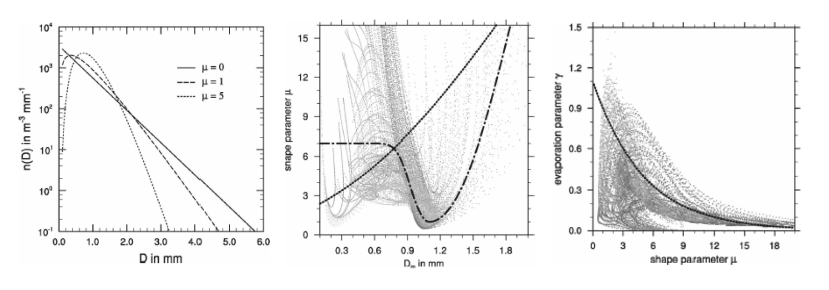
\includegraphics[scale=0.75]{./figure/mod_gamma_dist.eps}
\end{center}
\caption{Left figure shows the modified Gamma distribution for various shape parameters μm. Center figure shows the scatter plot of shape parameter and mean volume diameter for various initial conditions. Gray dots are from the cloud model, dotted line is parameterization of Milbrandt and Yau (2005), and dashed-dotted line is that of Seifert (2008). Right figure shows the scatter plot of evaporation and shape parameters. These are from Seifert (2008).}
\label{figsn2-17}
\end{figure}

\begin{figure}[htbp]
\begin{center}
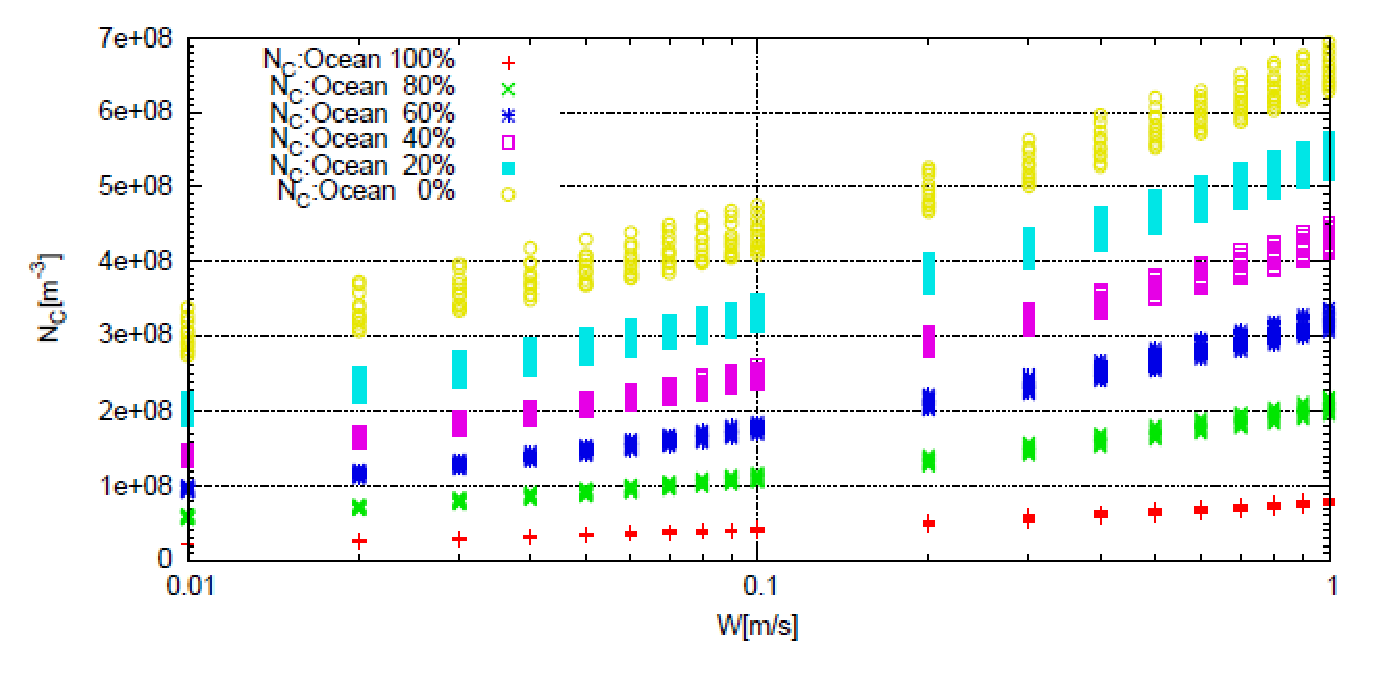
\includegraphics[scale=0.5]{./figure/density_max_num.eps}
\end{center}
\caption{Dependency of maximum number concentration on updraft velocity in ascending air parcel. These are based on a Twomey equation with various CCN conditions. Aerosol activation spectrum refers to eq.\ref{sn107}.}
\label{figsn2-18}
\end{figure}

\begin{figure}[htbp]
\begin{center}
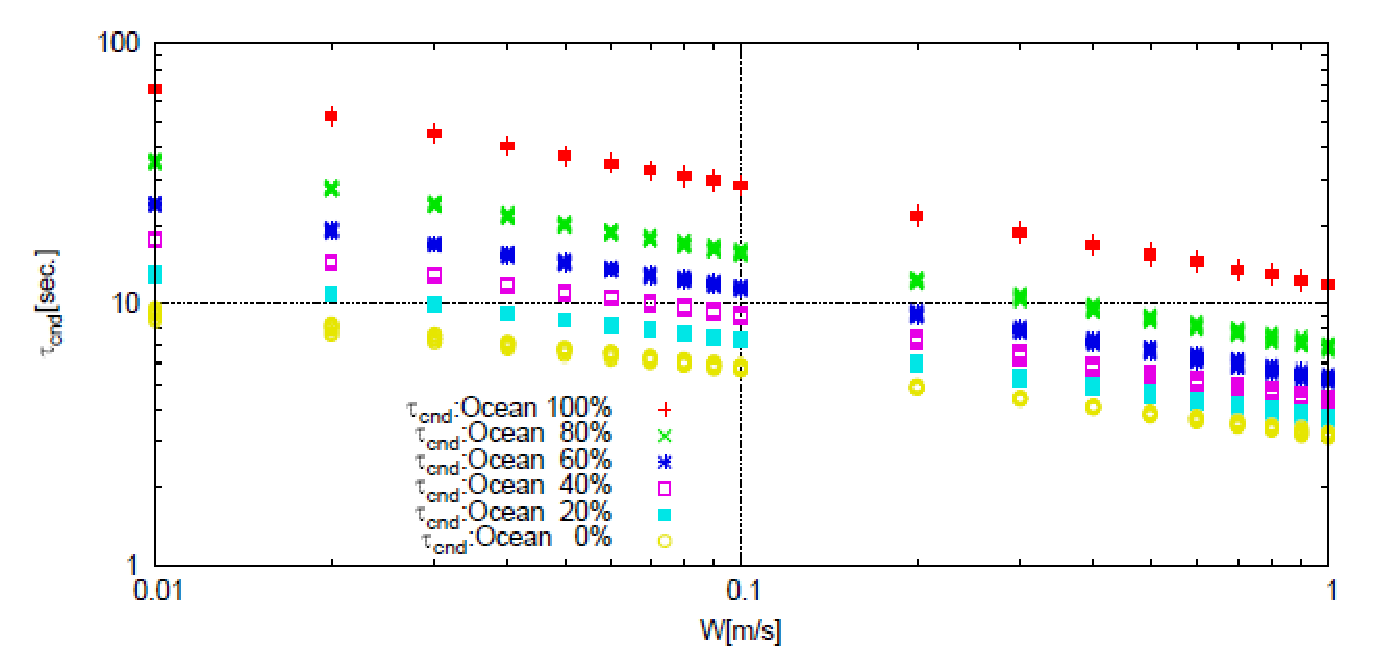
\includegraphics[scale=0.5]{./figure/cond_timescale.eps}
\end{center}
\caption{Timescale of condensation for cloud droplets at maximum number concentration in ascending air parcel. Experimental design is the same as Fig.\ref{figsn2-18}.}
\label{figsn2-19}
\end{figure}

\begin{figure}[htbp]
\begin{center}
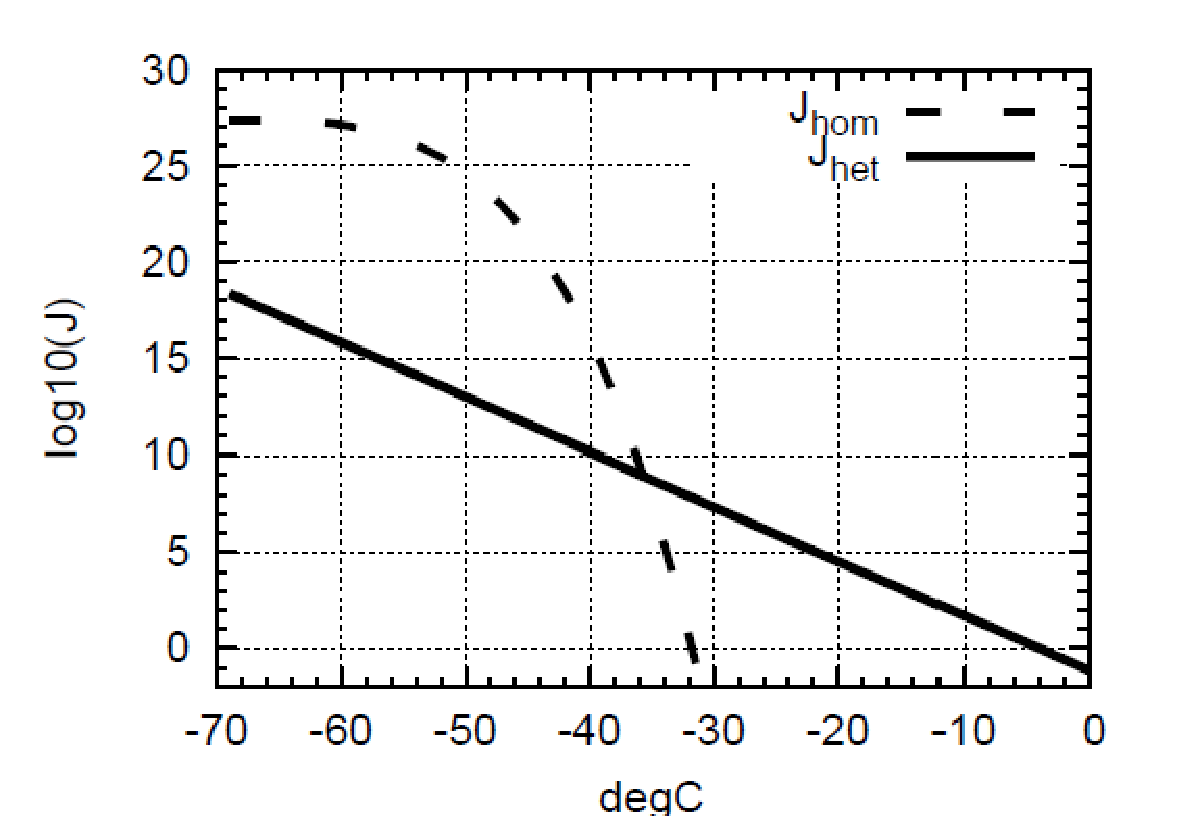
\includegraphics[scale=0.5]{./figure/homo_frz_rate.eps}
\end{center}
\caption{Dependencies of homogeneous freezing rate (dashed line) and heterogeneous freezing rate (solid line) on centigrade temperature. Freezing rates are in common logarithmic scale.}
\label{figsn2-20}
\end{figure}

\begin{figure}[htbp]
\begin{center}
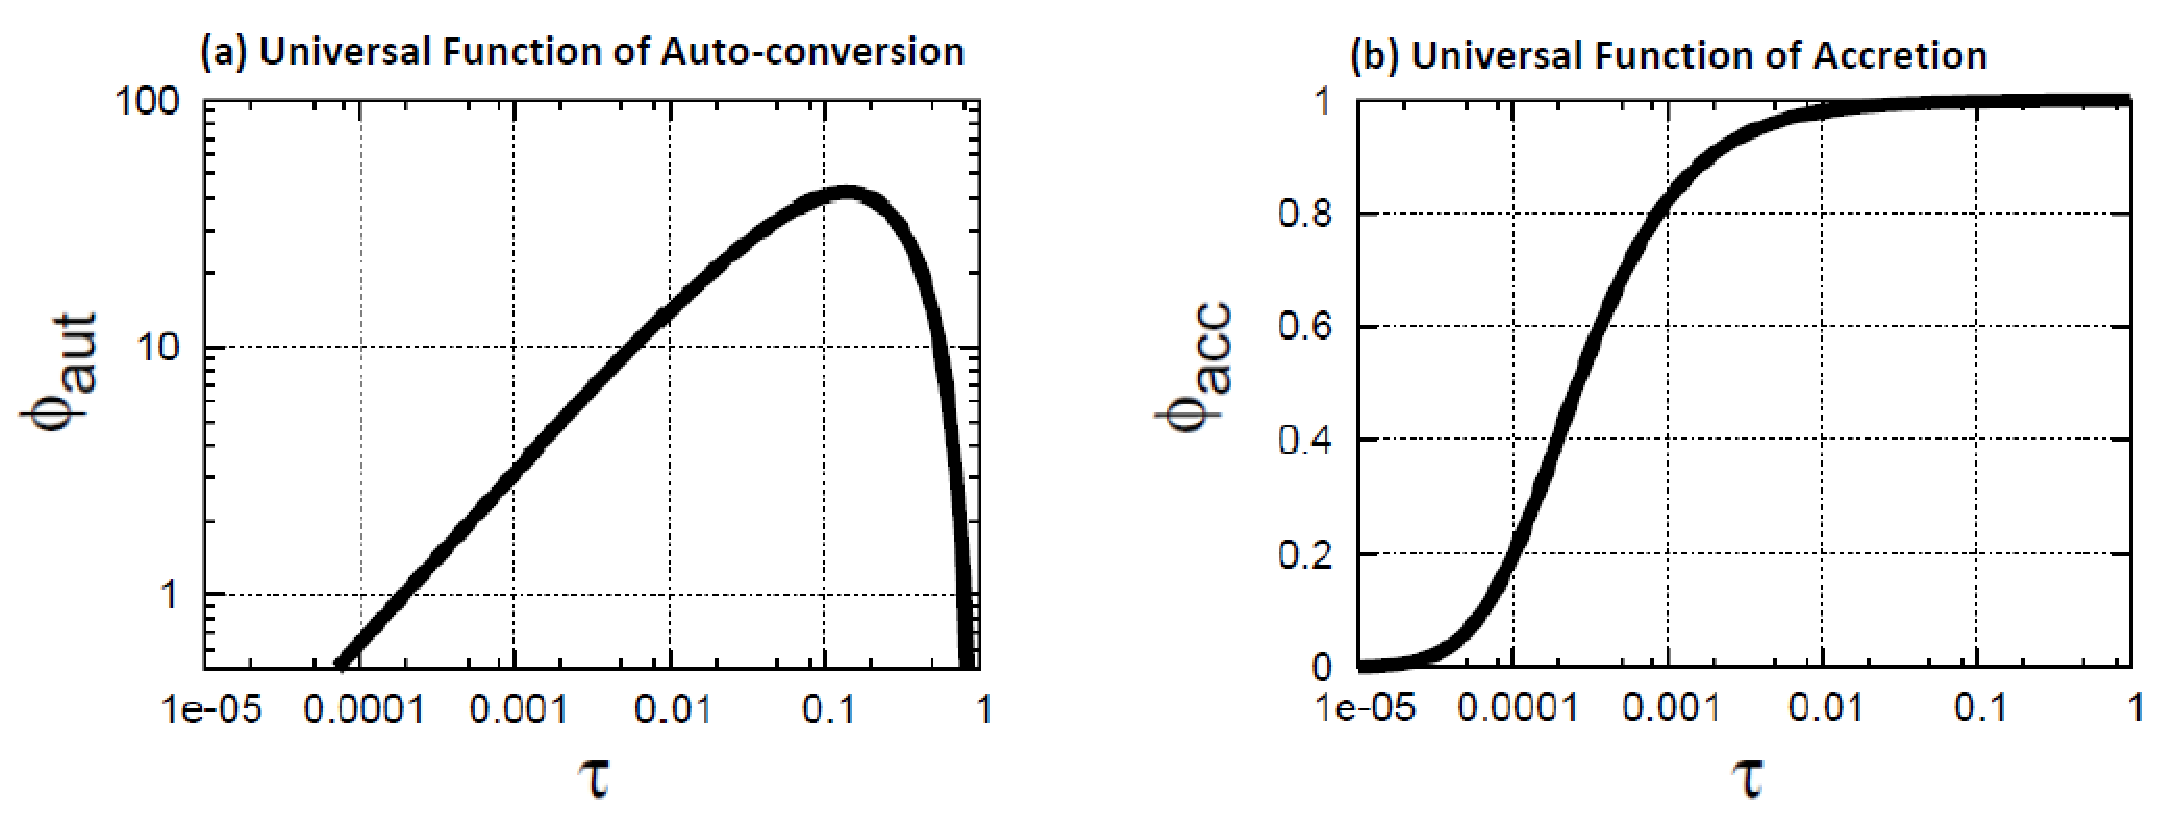
\includegraphics[scale=0.25]{./figure/univ_function.eps}
\end{center}
\caption{The universal functions of (a) auto-conversion and (b) accretion as a function of the dimensionless internal time scale.}
\label{figsn2-21}
\end{figure}

\begin{figure}[htbp]
\begin{center}
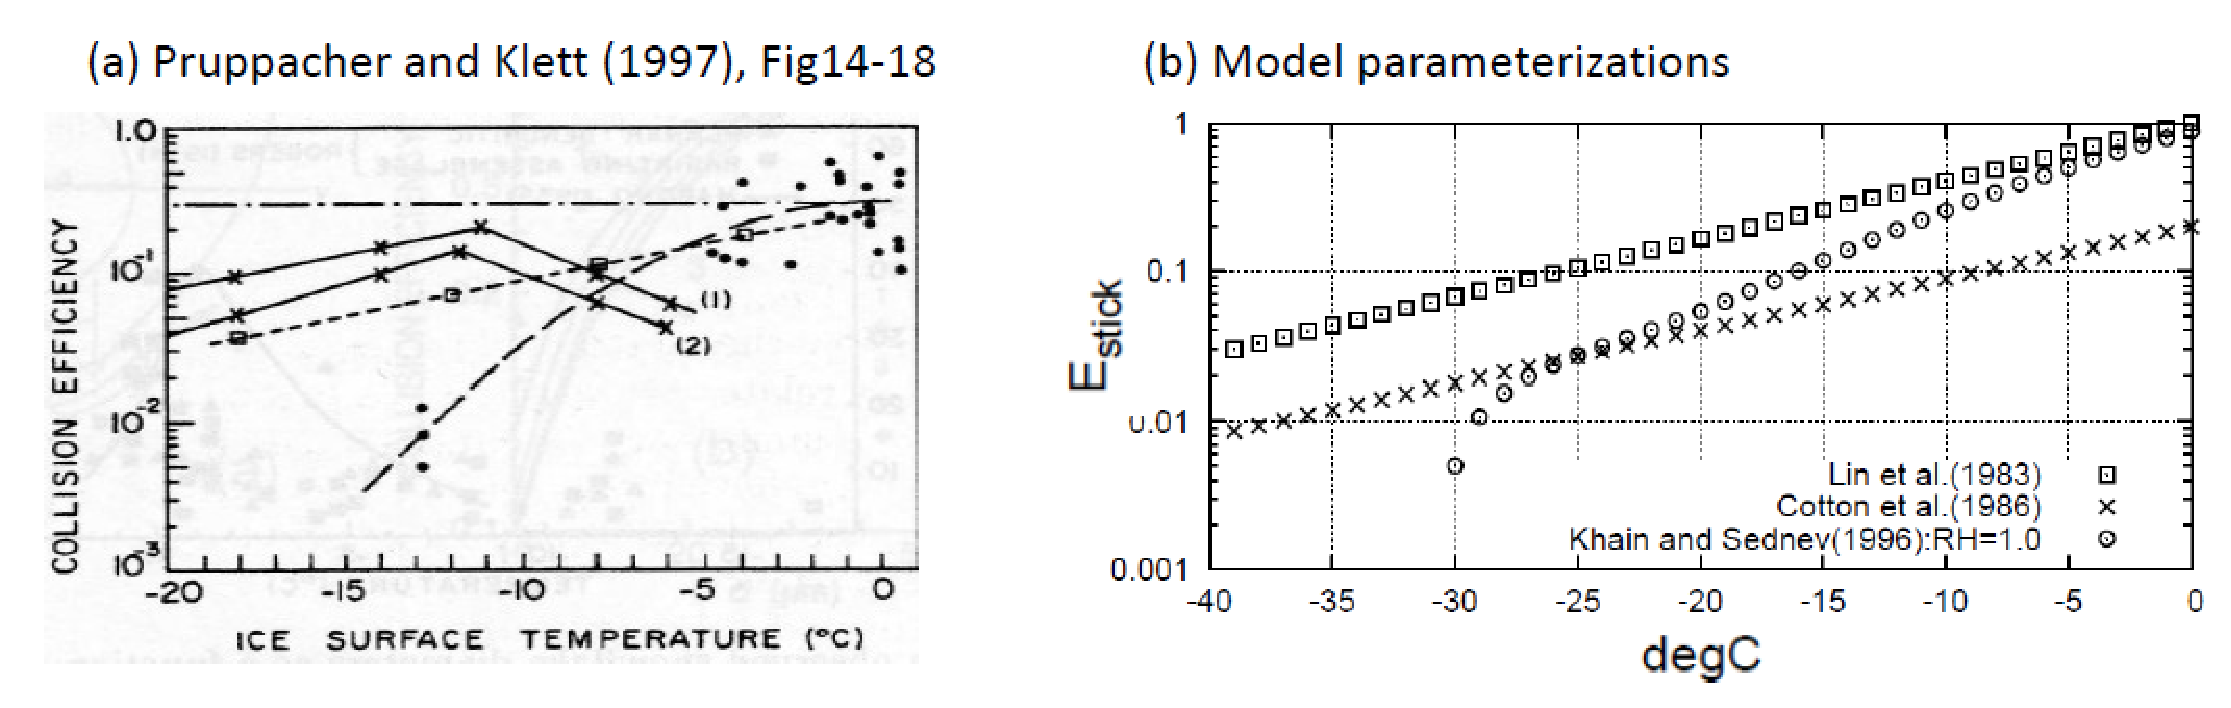
\includegraphics[scale=0.25]{./figure/stic_effic.eps}
\end{center}
\caption{Dependency of sticking efficiencies on centigrade temperature. Sticking efficiencies based on (a) various observations from Pruppacher and Klett (1997) and (b) model parameterizations.}
\label{figsn2-22}
\end{figure}

\begin{figure}[htpb]
\begin{center}
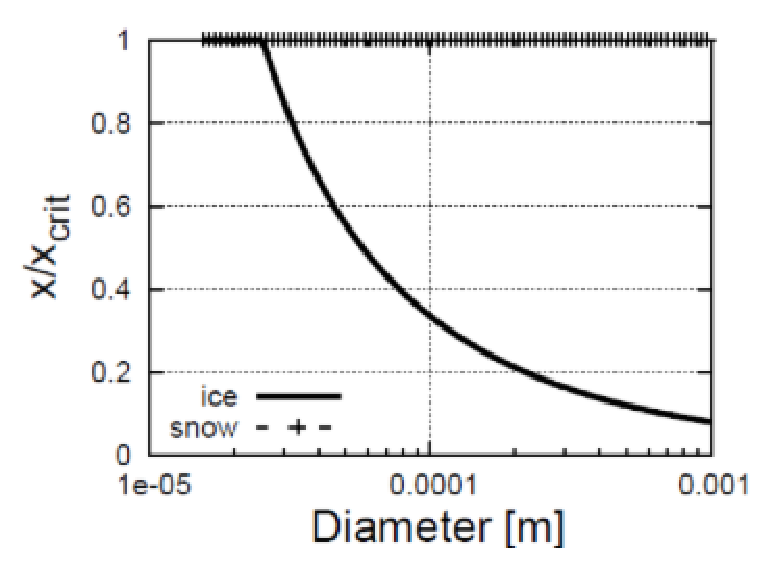
\includegraphics[scale=0.5]{./figure/partial_conversion_coef.eps}
\end{center}
\caption{Coefficients of partial conversion. Solid line shows the coefficient of ice and the line with symbol shows the coefficient of snow.}
\label{figsn2-23}
\end{figure}

\subsubsection{Appendix of Seiki and Nakajima (2014)}
\subsubsection{The k-th moment of generalized Gamma distribution}
The kth moment of the DSD frequently appears in cloud microphysics equations. In this section, we describe derivation of the kth moment of the generalized Gamma distribution. The generalized Gamma distribution is defined as $f(x) = \alpha x \nu exp(-\lambda x \mu)$. There are four parameters in this generalized Gamma distribution but only two prognostic moments in a CRM - the number concentration N and mass concentration L. Hence, $\mu$ and $\nu$ are set constant parameters so that the other coefficients $\alpha$ and $\lambda$ can be related to N and L, as follows:

\begin{eqnarray}
M^{0}=N&=&\alpha\int_{0}^{\infty}x^{\nu}exp(\lambda x^{\mu})dx\nonumber\\
&=&\frac{\alpha}{\lambda^{(\nu+1)/\mu}\mu}\int_{0}^{\infty}y^{(\nu+1)/\mu-1}exp(-y)dy,\;(y\equiv\lambda x^{\mu})\nonumber\\
&=&\frac{\alpha}{\lambda^{(\nu+2)/\mu}\mu}\Gamma\bigl(\frac{\nu+1}{\mu}\bigr)\label{sn255}\\
M^{1}=L&=&\frac{\alpha}{\lambda^{(\nu+2)/\mu}\mu}\Gamma\bigl(\frac{\nu+1}{\mu}\bigr)\nonumber
\end{eqnarray}

$\alpha$ is then expressed as:

\begin{eqnarray}
\alpha=\frac{N\mu\lambda^{(\nu+1)/\mu}}{\Gamma\bigl(\frac{\nu+1}{\mu}\bigr)}=\frac{L\mu \lambda^{(\nu+2)/\mu}}{\Gamma\bigl(\frac{\nu+2}{\mu}\bigr)}\nonumber
\end{eqnarray}

and we can derive $\lambda$ and $\alpha$:

\begin{eqnarray}
\lambda=\Bigl[\frac{\Gamma\bigl(\frac{\nu+1}{\mu}\bigr)}{\Gamma\bigl(\frac{\nu+2}{\mu}\bigr)}\Bigr]^{-\mu}\bar{x}^{-\mu}\;\;and\;\;\alpha=\frac{\nu N}{\Gamma\bigl(\frac{\nu+1}{\mu}\bigr)}\lambda^{(\nu+1)/\mu}\label{sn256}
\end{eqnarray}

where $\bar{x}=L/N$ defines the mean particle mass. We can rewrite the generalized Gamma distribution by using N and L, in the following form:

\begin{eqnarray}
f(x)=\frac{N}{\bar{x}}\bigl(\frac{x}{\bar{x}}\bigr)^{\nu}\frac{\mu}{\Gamma\bigl(\frac{nu+1}{\mu}\bigr)}\Bigl[\frac{\Gamma\bigl(\frac{\nu+2}{\mu}\bigr)}{\Gamma\bigl(\frac{\nu+1}{\mu}\bigr)}\Bigr]^{\nu+1}\exp\Bigl[-\bigl[\frac{\Gamma((\nu+2)/\mu)}{\Gamma((\nu+1)/\mu)}\frac{x}{\bar{x}}\bigr]^{\mu}\Bigr]\label{sn257}
\end{eqnarray}

The kth moment of DSD is now given by the expansion of eq.\ref{sn255} and by using eq.\ref{sn256}:

\begin{eqnarray}
M^{k}=\frac{\Gamma\bigl(\frac{k+\nu+1}{\mu}\bigr)}{\Gamma\bigl(\frac{\nu+1}{\mu}\bigr)}\Bigl[\frac{\Gamma\bigl(\frac{\nu+1}{\mu}\bigr)}{\Gamma\bigl(\frac{\nu+2}{\mu}\bigr)}\Bigr]^{k}N\bar{x}^{k},\;\;(k\in R)
\end{eqnarray}



\subsection{Spectral Bin Model(SBM)\cite{suzuki_etal_2010}}
The Spectral Bin Model (SBM) was developed by Suzuki et al. (2010)\cite{suzuki_etal_2010}. The model forecasts the Size Distribution Function (SDF) of seven types of hydrometeors (liquid, plate-ice, columnar-ice, dendritic-ice, snow, graupel, and hail). \\
The SBM calculates mass density of the seven types of hydrometeor and one type of aerosol as their SDFs. The SDF of aerosol can be changed by advection and activation (i.e., nucleation from aerosol to cloud) processes. The SDF of hydrometeors can be changed by several growth processes (i.e., activation from aerosol to cloud, condensation/evaporation, collision/coagulation, freezing/melting, ice nucleation, riming, aggregation, advection, and gravitational falling). \\
The time evolution of SDF (number density) of aerosol ($f_{a}(m,t)$) and SDF (number density) of hydrometeor ($f_{c}(m,t)$) are shown as:

\begin{eqnarray}
\frac{\partial f^{(\mu)}_{c}(m,t)}{\partial t}&=&Adv\bigl[f^{(\mu)}_{c}(m,t)\bigr]+Grav\bigl[f^{(\mu)}_{c}(m,t)\bigr]+\Bigl[ \frac{\partial f^{(\mu)}_{c}(m,t)}{\partial t}\Bigr ]_{cloud\;microphysics}\label{s10-1}\\
\frac{\partial f_{a}(m_{a},t)}{\partial t}&=&Adv\bigl[f_{a}(m_{a},t)\bigr]+Grav\bigl[f_{a}(m_{a},t)\bigr]+\Bigl[ \frac{\partial f_{a}(m_{a},t)}{\partial t} \Bigr ]_{cloud\;microphysics}.\label{s10-2}
\end{eqnarray}

where $\mu$ shows type of hydrometeor (the seven types), and $Adv[]$, $Grav[])$ show change of SDF by  advection and gravitational falling. $\Bigl[ \Bigr]_{cloud\;microphysics}$ shows SDF changes by cloud microphysical processes.\\
The time evolution of $f_{c}^{(\mu)}(m,t)$, and $f_{a}(m,t)$ are shown as:

\begin{eqnarray}
\Bigl[ \frac{\partial f_{c}^{(\mu)}(m,t)}{\partial t}\Bigl]_{cloud\;microphysics}&=&\Bigl[\frac{\partial f_{c}^{(\mu)}(m,t)}{\partial t}\Bigr]_{activation}+\Bigl[\frac{\partial f_{c}^{(\mu)}(m,t)}{\partial t}\Bigr]_{cond/evap}\nonumber\\
&+&\Bigl[\frac{\partial f_{c}^{(\mu)}(m,t)}{\partial t}\Bigr]_{coll/coag/rim/agg}\nonumber\\
&+&\Bigl[\frac{\partial f_{c}^{(\mu)}(m,t)}{\partial t}\Bigr]_{frz}+\Bigl[\frac{\partial f_{c}^{(\mu)}(m,t)}{\partial t}\Bigr]_{melt}\nonumber\\
\Bigl[ \frac{\partial f_{a}(m_{a},t)}{\partial t}\Bigl]_{cloud\;microphysics}&=&\Bigl[\frac{\partial f_{a}(m_{a},t)}{\partial t}\Bigr]_{activation}\nonumber
\end{eqnarray}

where $\Bigl[\;\Bigr]_{***}$ show change of SDF by each cloud growth process. The detail of these processes will be provided later.\\
 The change of SDFs by advection and gravitational falling (i.e., first and second terms of eq. \ref{s10-1}, and \ref{s10-2}  ) are calculated by dynamical core of SCALE-RM shown in section 3.


\subsubsection{Discretization of Size Distribution Function(SDF)}
The SDF of aerosol and cloud is predicted as mass density of each particle size ($g_{a}(m_{a})$, $g_{c}^{(\mu)}(m)$). However most equations are given as equations of number density of cloud/aerosol ($f_{c}^{(\mu)}(m,t)$, $f_{a}(m_{a},t)$); the mass density of cloud/aerosol is transferred to the number density of cloud/aerosol ($g_{a}(m_{a},t)=m_{a}g_{a}(m_{a},t)$, $g_{c}^{(\mu)}(m,t)=m^{(\mu)}f_{c}^{(\mu)}(m,t)$).\\
To cover a wide size range (i.e., $2\;\mu m$ $\sim$ $3\;mm$), a logarithmically uniform grid system ($log(m)\equiv \eta$, $log(m_{a})\equiv \eta_{a}$) is used. In this system, the relationship, $\frac{m_{i+1}}{m_{i}}=const.$ is satisfied.

\subsubsection{Activation from aerosol to cloud particles (nucleation process)}
The change of SDFs by activation from aerosol to cloud particles is calculated based on Kohler theory (Kohler 1936). Through this process, aerosols with radii larger than the aerosol critical radius ($r_{a,crit}$) are activated to clouds. The critical radius is given as:

\begin{eqnarray}
r_{a,crit}=\bigl( \frac{4}{27}\frac{A^{3}}{B}\frac{1}{S_{w}}\Bigr )^{1/3}, \:\:\:A=\frac{2\sigma}{R_{v}\rho_{L}T},\:\:\: B=i_{v}\frac{M_{v}}{M_{s}}\frac{\rho_{s}}{\rho_{L}}.\label{s10-3}
\end{eqnarray}

where $S_{w}$, $\sigma$, $R_{v}$, $\rho_{L}$, $T$, $i_{v}$, $M_{v}$, $M_{s}$, and $\rho_{s}$ show supersaturation of water, surface tension of water, vapor gas constant, temperature, van't Hoff factor ($=2$), molecular weight of water, molecular weight of aerosol, and density of aerosol, respectively.\\
At each time step, $r_{a,crit}$ is calculated using temperature, and masses of aerosols with radii > $r_{a,crit}$ are removed from SDF of aerosol and 
transferred to SDF of cloud as newly generated cloud particles.\\
The radii of newly generated clouds correspond to those of aerosols, but if the radii of aerosols are smaller than the lower limit of cloud SDF, the radii of newly generated clouds are set to the smallest size of cloud SDF ($\sim 2 \mu m$).\\
The changes in aerosol and hydrometeor SDF are shown as:

\begin{eqnarray}
\Bigl[\frac{\partial f_{a}}{\partial t}\Bigr]_{activation}&=&-\int_{m_{a,crit}}^{\infty}f_{a}(m_{a},t)dm_{a}\label{s10-4}\\
\Bigl[\frac{\partial f_{c}^{(\mu)}}{\partial t}\Bigr]_{activation}&=&-\Bigl[\frac{\partial f_{a}}{\partial t}\Bigr]_{activation}\label{s10-5}
\end{eqnarray}

where $m_{a,crit}=\bigl(=\frac{4\pi}{3}r_{a}^{3}\rho_{a}$ is mass of aerosol particles with radii the same as critical radii, $r_{a,crit}$. When there is not enough vapor to activate all aerosol particles with radii larger than the critical radius, i.e.,

\begin{eqnarray}
\int_{m_{a,crit}}^{\infty}m_{a}f_{a}(m_{a},t)dm_{a} > q_{v}\rho,\label{s10-6}
\end{eqnarray}

only the aerosol particles with radii > than $r_{a0,crit}$, given as:

\begin{eqnarray}
\int_{m_{a0,crit}}^{\infty}m_{a}f_{a}(m_{a},t)dm_{a} = q_{v}\rho,\label{s10-7}
\end{eqnarray}


are transferred to cloud particles as:

\begin{eqnarray}
\Bigl[\frac{\partial f_{a}}{\partial t}\Bigr]_{activation}&=&-\int_{m_{a0,crit}}^{\infty}f_{a}(m_{a},t)dm_{a},\label{s10-8}\\
\Bigl[\frac{\partial f_{c}^{(\mu)}}{\partial t}\Bigr]_{activation}&=&-\Bigl[\frac{\partial f_{a}}{\partial t}\Bigr]_{activation}.\label{s10-9}
\end{eqnarray}

where $q_{v}$ and $\rho$ is the mixing ratio of water vapor and density.

\subsubsection{Condensation/evaporation}
Calculation of condensation and evaporation processes is based on an equation. The mass change by these two process is given by an equation (e.g., Rogers and Yau, 1989\cite{ry_1989}):

\begin{eqnarray}
\frac{dm}{dt}&=&C^{(\mu)}(m)G^{(\mu)}(T)S^{(\mu)}\\
G^{(\mu)}(T)&=&
\left\{
\begin{array}{l}
G_{w}(T)\;\;\;(\mu : \:liquid)\\
G_{i}(T)\;\;\;(\mu : \:ice)
\end{array}\right. \nonumber\\
G_{w}(T)&=&\frac{4\pi}{\frac{R_{v}T}{e_{w}(T)D_{v}}+\frac{L_{w}}{KT}\bigl( \frac{L_{w}}{R_{v}T}-1\Bigr )}\nonumber\\
G_{i}(T)&=&\frac{4\pi}{\frac{R_{v}T}{e_{i}(T)D_{v}}+\frac{L_{i}}{KT}\bigl( \frac{L_{i}}{R_{v}T}-1\Bigr )}\nonumber\\
S^{(\mu)}&=&
\left\{
\begin{array}{l}
S_{w}\;\;\;(\mu : liquid)\\
S_{i}\;\;\;(\mu : ice)
\end{array}\right.\nonumber
\end{eqnarray}

where $C^{(\mu)}(m)$ is capacitance, which depends on the shape of each type of hydrometeor, $S_{w}$, $S_{i}$ are super saturation of water and ice, $L_{w}$, $L_{i}$ are sensible heat of evaporation, sublimation, $D_{v}$ is diffusion constant of vapor, $K$ is conductivity of air, and $e_{w}$, $e_{i}$ are saturation vapor pressure and saturation ice pressure, respectively. Condensation (evaporation) occur when $S^{(\mu)}$ is positive (negative).\\
To calculate change of SDF by condensation/evaporation, mass flux ($F^{(\mu)}_{cond/evap}$) on each bin is given by using number density ($f_{c}^{(\mu)}$) and $\frac{dm}{dt}$ as:

\begin{eqnarray}
F^{(\mu)}_{cond/evap}=f^{(\mu)}(m)\frac{dm}{dt}=f^{(\mu)}(m)C^{(\mu)}G^{(\mu)}(T)S^{(\mu)}.\label{s10-10}
\end{eqnarray}

Using this equation, time evolution of SDF ($f^{(\mu)}$) is given as

\begin{eqnarray}
\Bigl[\frac{\partial f^{(\mu)}(m,t)}{\partial t}\Bigr]_{cond/evap}&=&-\frac{\partial}{\partial m}F^{(\mu)}_{cond/evap}(m)\nonumber\\
&=&-\frac{\partial}{\partial m}\bigl (f^{(\mu)}(m)C^{(\mu)}\bigr ) G^{(\mu)}(T)S^{(\mu)}.\label{s10-11}
\end{eqnarray}


By using the $\eta(=\log(m))$, eq.\ref{s10-11} is transferred to the advection equation :

\begin{eqnarray}
\frac{\partial f^{(\mu)}(\eta)}{\partial t}&=&-\frac{\partial}{\partial \eta}\bigl ( f^{(\mu)}(\eta)U^{(\mu)}(\eta)\bigr)\label{s10-12}\\
U^{(\mu)}(\eta)&=&\frac{C^{(\mu)}(\eta)}{\exp (\eta)}G^{(\eta)}(T)S^{(\eta)}.\nonumber
\end{eqnarray}

To solve eq. \ref{s10-12}, a scheme developed by Bott (1989)\cite{bott_1989} is used. The number density of the i-th bin after $\Delta t$ ($f_{i}(t+\Delta t)$) is given as follows:

\begin{eqnarray}
f_{i}(t+\Delta t)&=&f_{i}(t)-\frac{\Delta t}{\Delta \eta}\bigl [F_{cond/evap,i+1/2}-F_{cond/evap,i-1/2}\Bigr ].\nonumber\\
F_{cond/evap,i+1/2}&=&\frac{\Delta \eta}{\Delta t}\Bigl[ \frac{i^{+}_{l,i+1/2}}{i_{l,j}}f_{i}(t)-\frac{i^{-}_{l,i+1/2}}{i_{l,i+1}}f_{i+1}(t)\Bigr ]\nonumber\\
i^{+}_{l,i+1/2}&=&max\bigl(0,I^{+}_{l}(c_{i+1/2})\bigr)\nonumber\\
i^{-}_{l,i+1/2}&=&max\bigl(0,I^{-}_{l}(c_{i+1/2})\bigr)\nonumber\\
i^{+}_{l,i}&=&max\bigl(I_{l,i},i^{+}_{l,i+1/2}+i^{-}_{l,i+1/2})\bigr)\nonumber\\
I^{+}_{l}(c_{i+1/2})&=&\sum_{k=0}^{2}\frac{a_{i,k}}{(k+1)2^{k+1}}\bigl[1-(1-2c^{+}_{j})^{k+1}\bigr]\nonumber\\
I^{-}_{l}(c_{i+1/2})&=&\sum_{k=0}^{2}\frac{a_{i+1,k}}{(k+1)2^{k+1}}(-1)^{k}\bigl[1-(1-2c^{-}_{j})^{k+1}\bigr]\nonumber\\
a_{i,0}&=&-\frac{1}{24}\bigl( f_{i+1}(t)-26f_{i}(t)+f_{i-1}(t) \bigr)\nonumber\\
a_{i,1}&=&\frac{1}{2}\bigl( f_{i+1}(t)-f_{i-1}(t) \bigr)\nonumber\\
a_{i,2}&=&\frac{1}{2}\bigl( f_{i+1}(t)-2f_{i}(t)+f_{i-1}(t) \bigr)\nonumber\\
c_{i}^{\pm}&=&\pm\bigl( c^{n}_{i+1/2}\pm | c^{n}_{i+1/2}|\bigr )/2\nonumber\\
c^{n}_{i+1/2}&=&U^{n}_{i+1/2}\frac{\Delta t}{\Delta \eta}
\end{eqnarray}

Since super saturation ($S^{(\mu)}$) can change during time step ($\Delta t$), we apply a method shown below to reflect the change of supersaturation during $\Delta t$.\\
Time evolution of supersaturation can be given by equations:

\begin{eqnarray}
\frac{d}{dt}\left(
\begin{array}{l}
S_{w}\\
S_{i}\\
\end{array}\right )
&=&
\left(
\begin{array}{cc}
a_{c/e}& b_{c/e}\\
c_{c/e}& d_{c/e}
\end{array}\right)
\left(
\begin{array}{l}
S_{w}\\
S_{i}
\end{array}\right)
=
A
\left(
\begin{array}{l}
S_{w}\\
S_{i}
\end{array}\right)\label{s10-13}\\
a_{c/e}&=&-(S_{w}+1)\Bigl(\frac{1}{q_{v}}+\frac{L_{w}}{R_{v}T^{2}}\frac{L_{w}}{C_{p}}\Bigr )\int f^{(w)}(m)C^{(w)}(m)dm G_{w}(t)\nonumber\\
b_{c/e}&=&-(S_{w}+1)\Bigl(\frac{1}{q_{v}}+\frac{L_{w}}{R_{v}T^{2}}\frac{L_{i}}{C_{p}}\Bigr ) \sum_{\mu \in ice}\int f^{(\mu)}(m)C^{(\mu)}(m)dm G_{i}(t)\nonumber\\
c_{c/e}&=&-(S_{i}+1)\Bigl(\frac{1}{q_{v}}+\frac{L_{i}}{R_{v}T^{2}}\frac{L_{w}}{C_{p}}\Bigr ) \int f^{(w)}(m)C^{(w)}(m)dm G_{w}(t)\nonumber\\
d_{c/e}&=&-(S_{i}+1)\Bigl(\frac{1}{q_{v}}+\frac{L_{i}}{R_{v}T^{2}}\frac{L_{i}}{C_{p}}\Bigr ) \sum_{\mu \in ice}\int f^{(\mu)}(m)C^{(^mu)}(m)dm G_{i}(t)\nonumber
\end{eqnarray}


where $q_{v}$ is the mixing ratio of vapor. \\
Using eigen value of $A$ ($\Lambda_{+}$, $\Lambda_{-}$ ($\Lambda_{+}>\Lambda_{-})$), and assuming $a_{c/e}$, $b_{c/e}$, $c_{c/e}$, $d_{c/e}$ are constant during $\Delta t$, average value of super saturation ($\bar{S}_{w,i}(t)$) during $\Delta t$ is given as:

\begin{eqnarray}
\bar{S}_{w}(t)=\frac{1}{\Delta t}\int_{t}^{t+\Delta t}S_{w}(\tau)d\tau&=&b\frac{e^{\Lambda_{+}\Delta t}-1}{\Lambda_{+}\Delta t}S_{+}(t)+b\frac{e^{\Lambda_{-}\Delta t}-1}{\Lambda_{-}\Delta t}S_{-}(t)\nonumber\\
\bar{S}_{i}(t)=\frac{1}{\Delta t}\int_{t}^{t+\Delta t}S_{i}(\tau)d\tau&=&(\Lambda_{+}-a)\frac{e^{\Lambda_{+}\Delta t}-1}{\Lambda_{+}\Delta t}S_{+}(t)+(\Lambda_{-}-a)\frac{e^{\Lambda_{-}\Delta t}-1}{\Lambda_{-}\Delta t}S_{-}(t)\nonumber\\
S_{+}(t)&=&\frac{(\Lambda_{-}-a)S_{w}(t)-bS_{i}(t)}{b(\Lambda_{-}-\Lambda_{+})}\nonumber\\
S_{+}(t)&=&\frac{(a-\Lambda_{+})S_{w}(t)+bS_{i}(t)}{b(\Lambda_{-}-\Lambda_{+})}\nonumber
\end{eqnarray}

The averaged super saturation ($\bar{S}_{w,i}(t)$) is used to solve the eq. \ref{s10-13}.

\subsubsection{Collision/coagulation/riming/aggregation}
Collision/coagulation processes are calculated by solving stochastic collision equations (e.g., Pruppecher and Klett, 1997)\cite{pk_1997}:

\begin{eqnarray}
\frac{\partial f(m)}{\partial t}&=&\int_0^{m/2}f(m')f(m-m')K(m',m-m')dm' \nonumber\\
&-&f(m)\int_0^{\infty}f(m'')K(m,m'')dm''\label{s10-14}
\end{eqnarray}

where $K(m,m')$ is collection kernel function. Three types of kernel function, i.e., Long type kernel (Long, 1974\cite{long_1974}), Golovin type kernel (Golovin, 1963\cite{Golovin_1963}), and Hydro-dynamic dynamic kernel as shown in eq. \ref{s10-15}, are implemented into the SCALE-RM.

\begin{eqnarray}
K(m,m')=\pi(r(m)-r(m'))\left| V(m)-V(m')\right |E_{col}(m,m')E_{coag}(m,m')\label{s10-15}
\end{eqnarray}

where $r(m)$ is radius of hydrometeors with mass $m$ and $V(m)$ is terminal velocity of hydrometeors. The terminal velocity of each species of hydrometeor and each size are shown in Figure \ref{figs10-term} $E_{col}$, and $E_{coag}$ are collision efficiency and coagulation efficiency, respectively.\\

\begin{figure}[ht]
\begin{center}
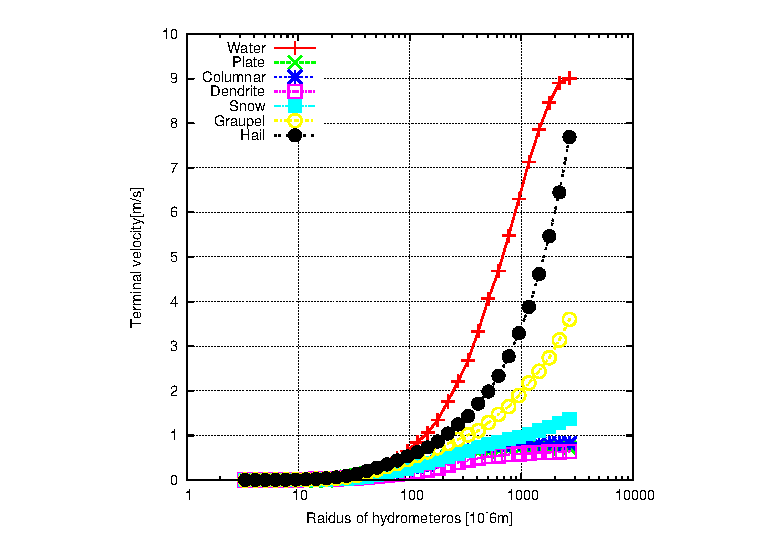
\includegraphics[scale=0.9]{./figure/terminal-velocity.eps}
\end{center}
\caption{Terminal velocity of Water (Plus), plate-type ice (cross), columnar-type ice (asterisk), dendritic-type ice (open square), snow (closed square), graupel (open circle), and hail (closed circle)}
\label{figs10-term}
\end{figure}


Although the stochastic collision equation can be applied for collision/coagulation of one type of hydrometeor (i.e., liquid water), SCALE-RM predicts seven types of hydrometeors and interactions of these types (i.e., riming/aggregation) must be calculated. To calculate the interaction of all seven types of hydrometeors, the extended stochastic collision equation:

\begin{eqnarray}
\Bigr[\frac{\partial f^{(\mu)}(m)}{\partial t}\Bigr]_{coll/coag/rim/agg}&=&\nonumber\\
\sum_{\lambda}\sum_{\nu}\int_{0}^{m/2}f^{(\lambda)}&(&m')f^{(\nu)}(m-m')K_{\lambda\nu}(m',m-m')dm' \nonumber\\
-f^{(\mu)}(m)\sum_{\kappa}\int_0^{\infty}f^{(\kappa)}&(&m'')K_{\kappa\mu}(m,m'')dm''\label{s10-16}
\end{eqnarray}

is applied (where $\mu$, $\nu$, $\lambda$, $\kappa$ represent species of hydrometeor). The combinations of $\mu$, $\nu$, $\lambda$ are shown in table \ref{table-s10-1}.

\begin{table}[h]
\begin{center}
\caption{Catalog of interaction between seven species. W, I, S, G, and H show water, ice, snow, graupel, and hail, respectively. G/H shows graupel(hail) generated when T is lower(higher) than 270.15}
\label{table-s10-1}
\begin{tabular}{cccccc}
\hline
     & W   & I   & S   & G   & H   \\ \hline\hline
W    & W   & G/H & G/H & G/H & G/H \\ \hline
I    & I   & S   & S   & I   & I   \\ \hline
S    & S   & S   & S   & S   & S   \\ \hline
G    & G/H & G/H & G   & G   & G/H \\ \hline
H    & G/H & G/H & G/H & G/H & H   \\ \hline
\end{tabular}
\end{center}
\end{table}


To solve the stochastic collision equation, a scheme developed by Bott (1998)\cite{bott_1998} was implemented into SCALE-RM.\\
The Bott (1998)\cite{bott_1998} scheme calculates evolution of mass density distribution ($g(\eta)=mf(\eta)$, $\eta=\log(m)$). The stochastic collision equation can be transferred to:

\begin{eqnarray}
\frac{\partial g(\eta)}{\partial t}&=&\int_{\eta_{0}}^{\eta_{1}}\frac{m^{2}}{(m-m')^{2} m'}g(\eta-\eta') K(\eta-\eta',\eta')g(\eta')d\eta' \nonumber\\
&-&\int_{\eta_{0}}^{\infty} g(\eta)\frac{K(\eta,\eta')}{m'}g(\eta')d\eta'.\label{s10-17}
\end{eqnarray}

 where $\eta_{1}=\log(m/2)$. Decreases of mass of i-th bin and j-th bin are given by:

\begin{eqnarray}
\frac{\partial g_{i}^{(\mu)}}{\partial t}=-\Delta g^{(\mu)}_{i} K_{\mu\nu}(i,j)\frac{g_{j}^{(\nu)}}{m_{j}}\Delta \eta\label{s10-18}
\end{eqnarray}

and


\begin{eqnarray}
\frac{\partial g_{j}^{(\mu)}}{\partial t}=-\Delta g^{(\nu)}_{j}K_{\mu\nu}(i,j)\frac{g_{i}^{(\mu)}}{m_{i}}\Delta \eta\label{s10-19}
\end{eqnarray}

respectively. The terms corresponds to the second term of the right-hand side of eq.\ref{s10-17}. Eqs. \ref{s10-18} and \ref{s10-19} can transfer to:

\begin{eqnarray}
\Delta g_{i}^{(\mu)}=g_{i}^{(\mu)}\Bigl [1-\exp\bigl(-K_{\mu\nu}(i,j)\frac{g^{(\nu)}_{j}}{m_{j}}\Delta \eta\Delta t\bigr) \Bigl]\label{s10-20}\\
\Delta g_{j}^{(\nu)}=g_{j}^{(\nu)}\Bigl [1-\exp\bigl(-K_{\mu\nu}(i,j)\frac{g^{(\mu)}_{i}}{m_{i}}\Delta \eta\Delta t\bigr) \Bigl].\label{s10-21}
\end{eqnarray}

The sum of $\Delta g_{i}^{(\mu)}$ and $\Delta g_{j}^{(\nu)}$ corresponds to newly generated mass by collision of hydrometeors with mass of $m_{i}$ and $m_{j}$. The newly generated mass ($g'=\Delta g_{i}^{(\mu)}+\Delta g_{j}^{(\nu)}$,  corresponds to the first term of the right-hand side of eq.\ref{s10-17}) added k-th bin ($m_{k}=m_{i}+m_{j}$). Since $m_{k}$ is not always bin center, newly generated mass is divided to the k-th and k+1-th bin, as follows.\\
The production of k-th and k+1-th bin is represented as:

\begin{eqnarray}
\Delta g_{k}^{(\lambda)}&=&g_{k}^{\lambda}+g'-\zeta\label{s10-22}\\
\Delta g_{k+1}^{(\lambda)}&=&g_{k+1}^{\lambda}+\zeta\label{s10-23}\\
\zeta&=&\frac{g'}{g_{k}^{(\lambda)}+g'}\sum_{s=0}^{2}\frac{a_{k,s}}{(s+1)2^{k+1}}[1-(1-2c_{k})^{k+1}]\nonumber\\
c_{k}&=&\frac{m'-m_{k}}{m_{k+1}-m_{k}}\nonumber\\
a_{k,0}&=&-\frac{1}{24}(g_{k+1}^{(\lambda)}-26g_{k}^{(\lambda)}+g_{k-1}^{(\lambda)})\nonumber\\
a_{k,1}&=&-\frac{1}{2}(g_{k+1}^{(\lambda)}-g_{k-1}^{(\lambda)})\nonumber\\
a_{k,2}&=&-\frac{1}{2}(g_{k+1}^{(\lambda)}-2g_{k}^{(\lambda)}+g_{k-1}^{(\lambda)})\nonumber
\end{eqnarray}

This procedure is applied for all bins of all types of hydrometeors.\\
In addition, for more rapid calculation, Sato et al. (2009)\cite{sato_etal_2009}’s scheme is also implemented into SCALE-RM.

\subsubsection{Freezing}
The calculation of the freezing process is based on a parameterization by Bigg (1953)\cite{bigg_1953}. The parameterization calculates number density of water ($f_{c}^{(w)}$) that can be frozen:

\begin{eqnarray}
\frac{\partial}{\partial t}f^{(w)}(m)&=&-\frac{f^{(w)}(m)}{\tau_{fr}}\label{s10-24}\\
\tau_{fr}&=&\frac{\exp \bigl[b_{fr}(T_{0}-T)\bigr]}{a_{fr} m}\nonumber
\end{eqnarray}

where $a_{fr}=10^{-4}s^{-1}$, and $b_{fr}=0.66^{o}C^{-1}$ are empirical parameters, and $T_{0}$ is 273.15 $K$.\\
Eq. \ref{s10-24} can transfer to:

\begin{eqnarray}
\frac{\partial g^{(w)(m)}}{\partial t}&=&-\frac{g^{(w)}(m)}{\tau_{fr}(m)}\\
\tau_{fr,i}&=&\frac{\exp\bigl (b_{fr}(T_{0}-T)\bigr )}{a_{fr}m}\nonumber
\end{eqnarray}

From this equation, the mass change of i-th bin during $\Delta t$ is given as:

\begin{eqnarray}
g_{i}^{(w)}(t+\Delta t)=g_{i}^{(w)}-Frz_{i}\\
\left \{
\begin{array}{r}
g_{i}^{(plate)}(t+\Delta t)=g_{i}^{(plate)}+Frz_{i}\:\:\: (r_{w}<200\mu m)\\
g_{i}^{(hail)}(t+\Delta t)=g_{i}^{(hail)}+Frz_{i}\:\:\: (r_{w}>200\mu m)
\end{array} \right.\label{s10-26}\\
Frz_{i}=g_{i}^{(w)}(t)\Bigl [1-\exp\bigl (-\frac{\Delta t}{\tau_{fr,i}}\bigr )\bigr]\nonumber
\end{eqnarray}


 As shown in eq. \ref{s10-26}, the mass of liquid is transferred from/to plate type ice ($r_{w}<200\mu m$) or hail ($r_{w}>200\mu m$).

\subsubsection{Melting}
The calculation of the melting process is too simple, with all ice particles (i.e., plate, columnar, dendritic, snow, graupel and hail) melting immediately when the temperature is > $T_{0}=273.15$ $K$. This is too simplistic to represent ice phase processes, and we will modify this method in the near future.




%\section{Radiation}
%{\Huge TBD}

\section{Surface flux}
%\section{Surface flux}
{\bf \Large 
\begin{tabular}{ccc}
\hline
  Corresponding author & : & Seiya Nishizawa\\
\hline
\end{tabular}
}


\subsection{Monin-Obukhov similarity}
The first of the all,
we assume that in the boundary layer
1. fluxes are constant,
and 2. variables are horizontally uniform.


Relations between flux and vertical gradient are
\begin{align}
  \frac{kz}{u_*} \frac{\partial u}{\partial z} &= \phi_m\left(\frac{z}{L}\right), \label{eq: flux-gradient u} \\
  \frac{kz}{\theta_*} \frac{\partial \theta}{\partial z} &= \phi_h\left(\frac{z}{L}\right), \label{eq: flux-gradient t} \\
  \frac{kz}{q_*} \frac{\partial q}{\partial z} &= \phi_q\left(\frac{z}{L}\right),
\end{align}
where $k$ is the Von Karman constant.
$L$ is the Monin-Obukhov scale height, which is
\begin{equation}
  L = \frac{\theta u_*^2}{kg\theta_*},
\end{equation}
where $g$ is the gravity.
The scaling velocity, $u_*$, temperature, $\theta_*$,
and water vapor, $q_*$, are defined
from the vertical eddy fluxes of momentum, sensible heat and water vapor:
\begin{align}
  \overline{u'w'} &= -u_*u_*, \\
  \overline{w'\theta'} &= - u_*\theta_*, \\
  \overline{w'q'} &= - u_*q_*.
\end{align}

The integration between the roughness length $z_0$ to the height $z$ of the lowest model level, eqs. (\ref{eq: flux-gradient u}) and (\ref{eq: flux-gradient t}) become
\begin{align}
  u(z) &= \frac{u_*}{k} \left\{\ln(z/z_0)-\Phi_m(z/L)+\Phi_m(z_0/L)\right\}, \\
  \Delta\theta &= R\frac{\theta_*}{k} \left\{\ln(z/z_0)-\Phi_h(z/L)+\Phi_h(z_0/L)\right\},
\end{align}
where $\Delta\theta = \theta-\theta_0$,
and
\begin{align}
  \Phi_m(z) = \int^z \frac{1-\phi_m(z')}{z'} dz', \\
  \Phi_h(z) = \int^z \frac{R-\phi_h(z')}{R z'} dz'.
\end{align}


\subsection{Louis (1979) Model}
Louis (1979) introduced a parametric model of vertical eddy fluxes.

The $L$ becomes
\begin{equation}
  L = \frac{\theta u^2}{g\Delta\theta}
    \frac{\ln(z/z_0)-\Phi_h(z/L)+\Phi_h(z_0/L)}{\left\{\ln(z/z_0)-\Phi_m(z/L)+\Phi_m(z/L)\right\}^2}.
\end{equation}
The bulk Richardson number for the layer $Ri_B$ is
\begin{equation}
  Ri_B = \frac{gz\Delta\theta}{\theta u^2},
\end{equation}
and its form implies relationship with the Monin-Obukhov scale height $L$.
Then the fluxes could be written as
\begin{align}
  u_*^2 &= a^2 u^2 F_m\left(\frac{z}{z_0},Ri_B\right), \label{eq: u_*^2} \\
  u_*\theta_* &= \frac{a^2}{R} u \Delta \theta F_h\left(\frac{z}{z_0},Ri_B\right), \label{eq: u_*t_*}
\end{align}
where
$R$ is ratio of the drag coefficients for momentum and heat in the neutral limit, and
\begin{equation}
  a^2 = \frac{k^2}{\left\{\ln\left(z/z_0\right)\right\}^2}
\end{equation}
is the drag coefficient in neutral conditions.

For the unstable condition ($Ri_B<0$),
$F_i$s ($i=m,h$) could be
\begin{equation}
  F_i = 1 - \frac{b Ri_B}{1 + c_i \sqrt{|Ri_B|}},
  \label{eq: F_i unstable}
\end{equation}
under the consideration that
$F_i$ must behave as $1/u$ (i.e. $\sqrt{|Ri_B|}$) in the free convection limit ($u \to 0$),
and becomes $1$ in neutral conditions ($Ri_B \to 0$).
In the stable conditions ($Ri_b$), on the other hand,
Louis (1979) adopted the following form for $F_i$:
\begin{equation}
  F_i = \frac{1}{(1 + b' Ri_B)^2}.
  \label{eq: F_i stable}
\end{equation}

The constants are estimated as
$R=0.74$ by Businger et al. (1971),
and $b=2b'=9.4$ by Louis (1979).
By the dimensional analysis,
\begin{equation}
  c_i = C^*_i a^2 b \sqrt{\frac{z}{z_0}},
\end{equation}
and $C^*_m = 7.4, C^*_h = 5.3$, which result best fit curves.


\subsection{Uno et al. (1995) Model}
Uno et al. (1995) extended the Louis Model,
which considers difference of the roughness length
between for momentum, $z_0$, and temperature, $z_t$.

The potential temperature difference between $z=z$ and $z=z_t$,
$\Delta\theta_t$, is
\begin{align}
  \Delta\theta_t
  &= R\frac{\theta_*}{k}\left\{\ln(z_0/z_t) - \Phi_h(z_0/L) + \Phi_h(z_t/L)\right\} + \Delta\theta_0, \nonumber \\
  &= R\frac{\theta_*}{k}{\ln(z_0/z_t)} + \Delta\theta_0, \nonumber \\
  &= \Delta\theta_0 \left\{\frac{R\ln(z_0/z_t)}{\Psi_h} + 1\right\},
\end{align}
where $\Delta\theta_0 = \theta_z - \theta_{z_0} (=\Delta\theta)$,
\begin{equation}
  \Psi_h = \int_{z_0}^z\frac{\phi_h}{z'}dz', \label{eq: Psi_h}
\end{equation}
and $\phi_h$ is assumed to be $R$ in the range $z_t < z < z_0$.
Thus
\begin{equation}
  \Delta\theta_0 = \Delta\theta_t \left\{\frac{R\ln(z_0/z_t)}{\Psi_h}+1\right\}^{-1},
  \label{eq: Delta t_0}
\end{equation}
or equivalently,
\begin{equation}
  Ri_{B0} = Ri_{Bt} \left\{\frac{R\ln(z_0/z_t)}{\Psi_h}+1\right\}^{-1}.
  \label{eq: Ri_B0}
\end{equation}

From the eqs. (\ref{eq: u_*^2}) and (\ref{eq: u_*t_*}),
\begin{equation}
  \Delta\theta_0 = \frac{R\theta_*}{k}\ln\left(\frac{z}{z_0}\right)\frac{\sqrt{F_m}}{F_h},
\end{equation}
while
\begin{equation}
  \Delta\theta_0 = \frac{\theta_*}{k}\Psi_h,
\end{equation}
from eqs. (\ref{eq: flux-gradient t}) and (\ref{eq: Psi_h}).
Therefore
\begin{equation}
  \Psi_h = R\ln\left(\frac{z}{z_0}\right)\frac{\sqrt{F_m}}{F_h}.
  \label{eq: Psi}
\end{equation}

Because $\Psi_h$ depends on $Ri_{B0}$,
$Ri_{B0}$ cannot be calculated from $Ri_{Bt}$ with eq. (\ref{eq: Ri_B0})
directly,
so numerical iteration is required to obtain $Ri_{B0}$
\footnote{In the stable case, it can be solved analytically
with eq. (\ref{eq: F_i stable}),
but the solution is too complicated.}.
Starting from $Ri_{Bt}$ as the first estimation of $Ri_{B0}$,
the second estimate by the Newton-Raphson iteration becomes
\begin{equation}
  \hat{Ri}_{B0} = Ri_{Bt} - \frac{Ri_{Bt}R\ln(z_0/z_t)}{\ln(z_0/z_t) + \hat{\Psi}_h},
  \label{eq: Ri_B0 estimation}
\end{equation}
where $\hat{\Psi}_h$ is the estimate of $\Psi_h$ using $Ri_{Bt}$ instead of $Ri_{B0}$.
Approximate values for $F_m, F_h$, and $\Psi_h$ are re-calculated
based on the $\hat{Ri}_{B0}$,
and then
$\Delta\theta_0$, and the surface fluxes $u_*^2$ and $u_*\theta_*$
are calculated from eqs. (\ref{eq: Delta t_0}), (\ref{eq: u_*^2}),
and (\ref{eq: u_*t_*}), respectively.


R\subsection{Roughness length}
Miller et al. (1992) provides the roughness length over the tropical ocean,
based on the numerical calculations
by combining the smooth surface values with the Charnock relation
for the aerodynamic roughness length
and the constant values for heat and moisture in accordance with Smith (1988,1989) suggestions:
\begin{align}
  z_0 &= 0.11u/\nu_* + 0.018u_*^2/g, \label{eq: z_0} \\
  z_t &= 0.40u/\nu_* + 1.4 \times 10^{-5}, \label{eq: z_t} \\
  z_q &= 0.62u/\nu_* + 1.3 \times 10^{-4}, \label{eq: z_q}
\end{align}
where $\nu_*$ is the kinematic viscosity of air ($\sim 1.5 \times 10^{-5}$),
and $z_0, z_t$, and $z_q$ are the roughness length
for the momentum, heat, and vapor, respectively.



\subsection{Discretization}

\def\half{\frac{1}{2}}

All the fluxes are calculated based on the velocity at the first full-level (k=1)
($z=\Delta z/2$).
The absolute velocities $U$ are
\begin{align}
  U_{i+\half,j,1}^2 &=
    \left\{\frac{2(\rho u)_{i+\half,j,1}}{\rho_{i,j,1}+\rho_{i+1,j,1}}\right\}^2
  + \left\{\frac{(\rho v)_{i,j-\half,1} + (\rho v)_{i,j+\half,1} + (\rho v)_{i+1,j-\half,1} + (\rho v)_{i+1,j+\half,1}}{2(\rho_{i,j,1}+\rho_{i+1,j,1})}\right\}^2 \nonumber \\
 &+ \left\{\frac{(\rho w)_{i,j,1+\half} + (\rho w)_{i+1,j,1+\half}}{2(\rho_{i,j,1}+\rho_{i+1,j,1})}\right\}^2, \\
  U_{i,j+\half,1}^2 &=
    \left\{\frac{(\rho u)_{i-\half,j,1} + (\rho u)_{i+\half,j,1} + (\rho u)_{i-\half,j-1,1} + (\rho u)_{i+\half,j+1,1}}{2(\rho_{i,j,1}+\rho_{i,j+1,1})}\right\}^2 \nonumber\\
 &+ \left\{\frac{2(\rho v)_{i,j+\half,1}}{\rho_{i,j,1}+\rho_{i,j+1,1}}\right\}^2
  + \left\{\frac{(\rho w)_{i,j,1+\half} + (\rho w)_{i,j+1,1+\half}}{2(\rho_{i,j,1}+\rho_{i,j+1,1})}\right\}^2, \\
  U_{i,j,1}^2 &=
    \left\{\frac{(\rho u)_{i-\half,j,1} + (\rho u)_{i+\half,j,1}}{\rho_{i,j,1}}\right\}^2
  + \left\{\frac{(\rho v)_{i,j-\half,1} + (\rho v)_{i,j+\half,1}}{\rho_{i,j,1}}\right\}^2
  + \left\{\frac{(\rho w)_{i,j,1+\half}}{2\rho_{i,j,1}}\right\}^2,
\end{align}
here it is note that $(\rho w)_{i,j,\half}=0$.
The potential temperatures $\theta$ are
\begin{align}
  \theta_{i,j,1} &= \frac{(\rho \theta)_{i,j,1}}{\rho_{i,j,1}}, \\
  \bar{\theta}_{i+\half,j,1} &= \frac{\theta_{i,j,1}+\theta_{i+1,j,1}}{2}, \\
  \bar{\theta}_{i,j+\half,1} &= \frac{\theta_{i,j,1}+\theta_{i,j+1,1}}{2}.
\end{align}

The roughness lengthes, $z_0, z_t$, and $z_q$ are caluclated from
the eqs. (\ref{eq: z_0}), (\ref{eq: z_t}), and (\ref{eq: z_q}),
in which the friction verociy $u_*$ is estimated as
\begin{equation}
  u_* = \frac{k}{\ln(z_1/z_0)}U.
\end{equation}

From eq. (\ref{eq: Ri_B0})
The $Ri_{Bt})$, which is the first guess of the $Ri_{B0}$, is
\begin{equation}
  Ri_{Bt} = \frac{gz_1(\theta_1-\theta_sfc)}{\Theta_{sfc}U^2},
\end{equation}
with the assumption that $\theta_{z_t} = \theta_{sfc}$.
The estimation of the $\hat{\Psi}_h$ is calculated with $Ri_{Bt}$ from
the eqs. (\ref{eq: Psi}), (\ref{eq: F_i unstable}), and (\ref{eq: F_i stable}).
The final estimation of $Ri_{B0}$ is obtained from the eq. (\ref{eq: Ri_B0 estimation}),
and the final estimation of $\Psi_h$ is obtaind with the $Ri_{B0}$.

Now we can calculate the bulk coefficients, $C_m, C_h$, and $C_e$ for the moments, heat, and vapor:
\begin{align}
  C_m &= \frac{k^2}{\ln(z_1/z_0)}F_m(Ri_{B0}), \\
  C_h &= \frac{k^2}{R\ln(z_1/z_0)}F_h(Ri_{B0})\left\{\frac{R\ln(z_0/z_t)}{\Psi_h}-1\right\}^{-1}, \\
  C_e &= \frac{k^2}{R\ln(z_1/z_0)}F_h(Ri_{B0})\left\{\frac{R\ln(z_0/z_e)}{\Psi_h}-1\right\}^{-1}.
\end{align}
The fluxes are
\begin{align}
  \overline{\rho u'w'} &= - C_m U \rho u, \\
  \overline{\rho v'w'} &= - C_m U \rho v, \\
  \overline{\rho w'w'} &= - C_m U \rho w, \\
  \overline{\rho \theta'w'} &= - C_h U \{\rho \theta - \rho \theta_{sfc}\}, \\
  \overline{\rho q'w'} &= -C_e U \rho ( q - q_{evap} ),
\end{align}
where $q_{evap}$ is the saturation value at surface.



\section{Land}
%\section{Land Physics}
{\bf \Large
\begin{tabular}{ccc}
\hline
  Corresponding author & :\\
  Tsuyoshi Yamaura and Seiya Nishizawa\\
\hline
\end{tabular}
}


\subsection{Bucket model}

The land bucket model estimates the soil temperature and soil moisture tendencies using a multi-layered bucket model.



\subsubsection{Soil moisture equation}

The conservation equations of the specific mass of the liquid and ice water (kg/m$^3$), $M_w$ and $M_i$, respectively, are
\begin{align}
  \frac{\partial M_w}{\partial t}
  &= - \frac{\partial}{\partial z} \left( F_w + F_{rain} - F_{evap} \right)
     - m_{frz} - m_{ro,w}, \label{eq:MwDt} \\
  \frac{\partial M_i}{\partial t}
  &= - \frac{\partial}{\partial z}\left( F_{snow} - F_{subl} \right) + m_{frz} - m_{ro,i}, \label{eq:MiDt}
\end{align}
where $\nu_w$ is the constant water diffusivity (m$^2$/s);
$\rho_w$ and $\rho_i$ are the dencity of liquid and ice water (kg/m$^3$), respectively;
$F_{rain}, F_{snow}, F_{evap}$ and $F_{subl}$ are the surface flux of rain, snow, evapolation, and sublimation (kg/m$^2$/s), respectively;
$m_{frz}$ and $m_{ro}$ are the mass change by freezing and the runoff of the water from the system (kg/m$^3$/s), respectively.
Note that the $F_{rain}$ and $F_{snow}$ are positive for the downward direction and the $F_{evap}$ and $F_{subl}$ are positive for the upward.
$F_w$ is the vertical flux due to the diffusion, and
\begin{align}
  F_w &= - \rho_w \nu_w\frac{\partial W}{\partial z}.
\end{align}
$W$ and $I$ are the soil moisture content (m$^3$/m$^3$) of liquid and ice water, respectively, and are
\begin{align}
 W &= \frac{M_w}{\rho_w}, \\
 I &= \frac{M_i}{\rho_i}.
\end{align}



The bucket model has the maximum soil mositure content $W_\mathrm{max}$, so if the moisture content is larger than the maximum, the moisuter runs off to the out of the system:
\begin{align}
 W + I \le W_\mathrm{max}.
\end{align}
Therefore, The amount of the runoff (kg/m$^3$) is estimated as
\begin{align}
 M_{ro} &= M_{ro,w} + M_{ro,i},
\end{align}
where
\begin{align}
 M_{ro,w} &= \int_t^{t+ \Delta t} m_{ro,w} dt = \rho_w \min\{W_{ro},W\}, \\
 M_{ro,i} &= \int_t^{t+ \Delta t} m_{ro,i} dt = \rho_i (W_{ro} - \min\{W_{ro},W\}),
\end{align}
and $W_{ro} = \max\{W + I - W_\mathrm{max}, 0\}$.

  

\subsubsection{Thermodynamical equation}

The total internal energy is the sum of that of the soil, liquid water and ice water, $U_s, U_w$ and $U_i$, respectively:
\begin{align}
 U &= U_s + U_w + U_i, \\
 U_s &= C_s T, \\
 U_w &= c_l T \rho_w W, \\
 U_i &= ( c_i T - L_f ) \rho_i I,
\end{align}
where $T$ is the soil temperature (K).
Note that, the temperature is
\begin{align}
 T &= \frac{U + L_f \rho_i I }{C_L},
\end{align}
where $C_L$ is the total heat capacity (J/K/m$^3$) and
\begin{align}
 C_L &= C_s + c_l \rho_w W + c_i \rho_i I.
\end{align}


The conservation equation of the total internal energy is
\begin{align}
 \frac{\partial U}{\partial t} &=
 - \frac{\partial}{\partial z} \left[
   - \kappa \frac{\partial T}{\partial z}
   + c_l T F_w  + F_{surf} \right]  \nonumber \\ &
 - c_l T M_{ro,w}
 - ( c_i T - L_f ) M_{ro,i}, \label{eq:UDt}
\end{align}
where $\kappa$ is the thermal conductivity (J/K/m/s).
$F_{surf}$ is the ground surface flux, and
\begin{align}
 F_{surf} &= G
 + c_l T_{rain} F_{rain}
 - c_l T_{evap} F_{evap} \nonumber \\&
 + ( c_i T_{snow} - L_f ) F_{snow},
 - ( c_i T_{subl} - L_f ) F_{subl},
\end{align}
where $G$ is the downward ground heat flux (J/m$^2$/s); and $T_{rain}, T_{evap}, T_{snow}$ and $T_{subl}$ are the temperature of the rain, evaporation water, snow, and sublimation ice, respectively.
These ground surface fluxes are calculated in the surface scheme.


The thermal conductivity depends on the moisture content, and Kondo and Saigusa 1994) gived it empirically as
\begin{align}
  \kappa &= \kappa_s + 0.5 W^\frac{1}{3},
\end{align}
where $\kappa_s$ is the thermal conductivity of the soil particle.



\subsubsection{Phase change}
The liquid water and ice water can exist instantenously only at the temperature $T_0$.
If the internal energy is lower than $C_sT_0 + (c_i T_0 - L_f) M$, all the moisutre is ice, where $M$ is the total moisture $M=M_w+M_i$.
On the other hand, the internal energy is larther than $C_sT_0 + c_lT_0M$, all the moisture is liquid.
Otherwize,
\begin{align}
 M_i &= \frac{U - ( C_s + c_l M ) T_0}{ (c_i-c_l)T_0 - L_f}, \\
 M_w &= M - M_i.
\end{align}
That is,
\begin{align}
 M_i &= \min\left\{ \max\left\{ \frac{U-(C_s+c_lM)T_0}{(c_i-c_l)T_0-L_f}, 0 \right\}, M \right\}, \\
 M_w &= M - M_i.
\end{align}


\subsubsection{Temporal integration}
Eqs. (\ref{eq:MwDt}, \ref{eq:MiDt} and \ref{eq:UDt}) are solved by a splitting method.
In the first step, the moisture mass and internal energy changes are calculated without the diffusion, runoff, and phase change.
In the second step, the phase change is calculated.
In the third step, the moisture diffusion equation is solved.
In the fouth step, the temperature diffusion is calculated with the thermal conductivity with the moisture content obtained in the second step.
At the last step, the runoff is calculated.


The followings are the summary of the sequence of calculation.
Here, the superscript ``$n$'' indicates the quantites at the time step $n$, ``$n_1$'', ``$n_2$'', ``$n_3$'', ``$n_4$'', and ``$n+1$'' are those after calculation of the first, seccond, third, fourth, and the last steps, respectively.
The vertical diffusion terms are calculated by the implicit scheme for numerical stability.

\begin{description}

\item[First step]

\begin{align}
 M^{n_1} &= \rho_w W^n + \rho_i I^n + \Delta t \frac{\partial}{\partial z}( F_{rain} + F_{snow} - F_{evap} - F_{subl} ), \\
 U^{n_1} &= C_L^n T^n - L_f \rho_i I^n + \Delta t \frac{\partial F_{surf}}{\partial z},
\end{align}
where $M$ is the total moisture mass (kg/m$^3$) and $M = M_w + M_i$.


\item[Second step]
\begin{align}
 M_i^{n_2} &= \min\left\{ \max\left\{ \frac{U^{n_1}-(C_s+c_lM^{n_1})T_0}{(c_i-c_l)T_0-L_f}, 0 \right\}, M^{n_1} \right\}, \\
 M_w^{n_2} &= M^{n_1} - M_i^{n_2}, \\
 W^{n_2} &= \frac{M_w^{n_2}}{\rho_w}, \\
 I^{n_2} &= \frac{M_i^{n_2}}{\rho_i}, \\
 T^{n_2} &= \frac{U^{n_1} + L_f M_i^{n_2}}{C_s + c_l M_w^{n_2} + c_i M_i^{n_2}}.
\end{align}


\item[Third step]
\begin{align}
 F_w &= - \rho_w\nu_w\frac{\partial W^{n_3}}{\partial z}, \\
 W^{n_3} &= W^{n_2} - \frac{\Delta t}{\rho_w} \frac{\partial F_w}{\partial z}, \\
 U^{n_3} &= U^{n_1} - \Delta t \frac{\partial c_l F_w T^{n_2}}{\partial z}, \\
 C_L^{n_3} &= C_s + c_l \rho_w W^{n_3} + c_i M_i^{n_2}.
\end{align}

\item[Fourth step]
\begin{align}
 \kappa &= \kappa_s + 0.5 (W^{n_3})^\frac{1}{3}, \\
 C_L^{n_3} T^{n+1} &= U^{n_3} + L_f M_i^{n_2}
 - \Delta t \frac{\partial}{\partial z} \left( -\kappa \frac{\partial T^{n+1}}{\partial z} \right).
\end{align}



\item[Fifth step]
\begin{align}
 I^{n+1} &= \min\{ I^{n_2}, W_\mathrm{max} \}, \\
 W^{n+1} &= \min\{ W_\mathrm{max} - I^{n+1}, W^{n_3} \}, \\
 M_{ro,w} &= \rho_w ( W^{n+1} - W^{n_3} ), \\
 M_{ro,i} &= \rho_i ( I^{n+1} - I^{n_2} )
\end{align}

\end{description}


\subsubsection{Descretization}
The moisture diffusion in the third step is solved as
\begin{align}
 W_1^{n_3} &= W_1^{n_2} + \frac{2\Delta t \nu_w }{\Delta z_1}\frac{W_2^{n_3} - W_1^{n_3}}{\Delta z_2 + \Delta z_1}, \\
 W_k^{n_3} &= W_k^{n_2} + \frac{2\Delta t \nu_w }{\Delta z_k}\left( \frac{W_{k+1}^{n_3} - W_k^{n_3}}{\Delta z_{k+1}+\Delta z_k}  - \frac{W_k^{n_3} - W_{k-1}^{n_3}}{\Delta z_k+\Delta z_{k-1}} \right), \\
 W_m^{n_3} &= W_m^{n_2} - \frac{2\Delta t \nu_w }{\Delta z_m}\left( \frac{W_m^{n_3} - W_{m-1}^{n_3}}{\Delta z_m+\Delta z_{m-1}} \right),
\end{align}
where the subscription $k$ represents that $W_k$ is the moisture content in the $k$-layer, and $k = 1, \cdots, m$, where $m$ is the number of the layers.
This can be written in the matrix form as
\begin{equation}
\begin{pmatrix}
  c_1  & b_1    &        &        &        &         &         \\
       & \ddots & \ddots & \ddots &        &         &         \\
       &        & a_k    & c_k    & b_k    &         &         \\
       &        &        & \ddots & \ddots & \ddots  &         \\
       &        &        &        &        & a_m     & c_m     \\
\end{pmatrix}
\begin{pmatrix}
  W_1^{n_1}   \\
  \vdots      \\
  W_k^{n_1}   \\
  \vdots      \\
  W_m^{n_1}   \\
\end{pmatrix}
=
\begin{pmatrix}
  V_1 \\
  \vdots        \\
  V_k \\
  \vdots        \\
  V_m
\end{pmatrix}
,
\end{equation}
where
\begin{align}
 V_k &= W_k^{n_2}, \\
 a_k &= - \frac{2\Delta t\nu_w}{\Delta z_k (\Delta z_k + \Delta z_{k-1})}, \\
 b_k &= - \frac{2\Delta t\nu_w}{\Delta z_k (\Delta z_{k+1} + \Delta z_k)}, \\
 c_k &= 1 - a_k - b_k.
\end{align}
This matrix can be solved by the Thomas algorithm (tridiagonal matrix algorithm).





The thermodynamical diffusion in the fourth step is discretized as
\begin{align}
  \kappa_k &= \kappa_s + 0.5 (W^{n_3}_k)^\frac{1}{3}, \\
%
  (F_w)_{k+\frac{1}{2}} &= - 2\rho_w\nu_w\frac{W^{n_3}_{k+1}-W^{n_3}_k}{\Delta z_{k+1}+\Delta z_k}, \\
%
  (C_L^{n_3})_1 T^{n+1}_1 &= U^{n_3}_1 + L_f(M_i)^{n_2}_1
  + \frac{\Delta t}{\Delta z_1} (\kappa_2+\kappa_1) \frac{T^{n+1}_2-T^{n+1}_1}{\Delta z_2+\Delta z_1}, \\
%
  (C_L^{n_3})_k T^{n+1}_k &= U^{n_3}_k + L_f(M_i)^{n_2}_k  \nonumber\\&
  + \frac{\Delta t}{\Delta z_k} \left( (\kappa_{k+1}+\kappa_k) \frac{T^{n+1}_{k+1}-T^{n+1}_k}{\Delta z_{k+1}+\Delta z_k} - (\kappa_k+\kappa_{k-1}) \frac{T^{n+1}_k-T^{n+1}_{k-1}}{\Delta z_k+\Delta z_{k-1}} \right), \\
%
  (C_L^{n_3})_m T^{n+1}_m &= U^{n_3}_m + L_f(M_i)^{n_2}_m
  - \frac{\Delta t}{\Delta z_m} (\kappa_m+\kappa_{m-1}) \frac{T^{n+1}_m-T^{n+1}_{m-1}}{\Delta z_m+\Delta z_{m-1}}.
\end{align}

As in the case of the soil moisture, the tendency equations can be solved using the Thomas algorithm.
\begin{align}
 V_k &= U^{n_3}_k + L_f (M_i)^{n_2}_k, \\
 a_k &= - \frac{\Delta t (\kappa_k+\kappa_{k-1})}{\Delta z_k(\Delta z_k+\Delta_{k-1})}, \\
 b_k &= - \frac{\Delta t (\kappa_{k+1}+\kappa_k)}{\Delta z_k(\Delta z_{k+1}+\Delta_k)}, \\
 c_k &= (C_L^{n_1})_k - a_k - b_k.
\end{align}



%\section{Aerosol}
%{\bf \Large
\begin{tabular}{ccc}
\hline
  Corresponding author & : & Mizuo Kajino\\
\hline
\end{tabular}
}


\section{Large scale sinking}
{\bf \Large 
\begin{tabular}{ccc}
\hline
  Corresponding author & : & Seiya Nishizawa\\
\hline
\end{tabular}
}


In the DYCOMS01 experiment, the large scale sinking is added
to express large scale downward motion corresponding to the Haddley circulation.
The motion converges virtually and results mass escape to out of the system.

The density loss rate is constant $L$:
\begin{equation}
  L = -\frac{\partial \rho w_L}{\partial z},
\end{equation}
where $w_l$ is vertical velocity corresponding to the large scale sinking.
Then vertical momentum with the sinking is
\begin{equation}
  \rho w_L = -Lz.
\end{equation}

Continuous equation is now
\begin{equation}
  \frac{\partial \rho}{\partial z}
  + \frac{\partial \rho u}{\partial x}
  + \frac{\partial \rho v}{\partial y}
  + \frac{\partial \rho (w+w_L)}{\partial z}
  = -L.
  \label{eq: lls rho}
\end{equation}

Lagrangian conservation equation for scalar quantities are
\begin{equation}
  \rho\frac{\partial \phi}{\partial t}
  + \rho u\frac{\partial \phi}{\partial x}
  + \rho v\frac{\partial \phi}{\partial y}
  + \rho (w+w_L)\frac{\partial \phi}{\partial z}
  = 0,
\end{equation}
and becomes with eq. (\ref{eq: lls rho})
\begin{equation}
  \frac{\partial \rho\phi}{\partial t}
  + \frac{\partial \rho u \phi}{\partial x}
  + \frac{\partial \rho v \phi}{\partial y}
  + \frac{\partial \rho (w+w_L) \phi}{\partial z}
  = -L\phi.
\end{equation}

The equations for mixing ratio is
\begin{equation}
  \frac{\partial \rho Q}{\partial t}
  + \frac{\partial \rho Q u }{\partial x}
  + \frac{\partial \rho Q v}{\partial y}
  + \frac{\partial \rho Q (w+w_L)}{\partial z}
  = -L Q.
\end{equation}
Note that this is identical to that of scalar quantities.

The $w_L$ at the top boundary is not zero while $w$ is zero.
The vertical flux $\rho w_L \phi$ at the top layer interface could be determined as
that convergence of the flux is canceled with $L\phi$.




\bibliographystyle{plainnat}
\bibliography{reference}

\appendix
\chapter{The detal numerics}
\section{4th order central differnce}
{
\footnotesize
The 4th order central difference is given by
\begin{eqnarray}
&& \frac{\partial \phi}{\partial x}
=\frac{-\phi_{i+2}+8\phi_{i+1}-8\phi_{i-1}+\phi_{i+2}}{12\Delta x} = 0
\end{eqnarray}
where
\begin{eqnarray}
&& \phi_{i+2} = \phi_{i}
+ 2 \Delta x \left(\frac{\partial \phi}{\partial x}\right)_{i}
+ 2 \Delta x^2 \left(\frac{\partial^2 \phi}{\partial x^2}\right)_{i}
+ \frac{4 \Delta x^3}{3} \left(\frac{\partial^3 \phi}{\partial x^3}\right)_{i}
+ \frac{2 \Delta x^4}{3} \left(\frac{\partial^3 \phi}{\partial x^4}\right)_{i}
+ O(\Delta x^5)\\
&& \phi_{i+1} = \phi_{i}
+ \Delta x \left(\frac{\partial \phi}{\partial x}\right)_{i}
+ \frac{\Delta x^2}{2} \left(\frac{\partial^2 \phi}{\partial x^2}\right)_{i}
+ \frac{\Delta x^3}{6} \left(\frac{\partial^3 \phi}{\partial x^3}\right)_{i}
+ \frac{\Delta x^4}{24} \left(\frac{\partial^3 \phi}{\partial x^4}\right)_{i}
+ O(\Delta x^5)\\
&& \phi_i = \phi_i\\
&& \phi_{i-1} = \phi_{i}
- \Delta x \left(\frac{\partial \phi}{\partial x}\right)_{i}
+ \frac{\Delta x^2}{2} \left(\frac{\partial^2 \phi}{\partial x^2}\right)_{i}
- \frac{\Delta x^3}{6} \left(\frac{\partial^3 \phi}{\partial x^3}\right)_{i}
+ \frac{\Delta x^4}{24} \left(\frac{\partial^3 \phi}{\partial x^4}\right)_{i}
+ O(\Delta x^5)\\
&& \phi_{i+2} = \phi_{i}
- 2 \Delta x \left(\frac{\partial \phi}{\partial x}\right)_{i}
+ 2 \Delta x^2 \left(\frac{\partial^2 \phi}{\partial x^2}\right)_{i}
- \frac{4 \Delta x^3}{3} \left(\frac{\partial^3 \phi}{\partial x^3}\right)_{i}
+ \frac{2 \Delta x^4}{3} \left(\frac{\partial^3 \phi}{\partial x^4}\right)_{i}
+ O(\Delta x^5)
\end{eqnarray}
Therefore,
\begin{eqnarray}
&&
\frac{-\phi_{i+2}+8\phi_{i+1}-8\phi_{i-1}+\phi_{i+2}}{12\Delta x}
= \left(\frac{\partial \phi}{\partial x}\right)_{i}+ O(\Delta x^4)\\
&&
\frac{(-\phi_{i+2}+7\phi_{i+1}+7\phi_{i}-\phi_{i-1})-
(-\phi_{i+1}+7\phi_{i}+7\phi_{i-1}-\phi_{i-2})}{12\Delta x}
= \left(\frac{\partial \phi}{\partial x}\right)_{i}+ O(\Delta x^4)
\end{eqnarray}


\section{Flux Corrected Transport scheme}
Equation (\ref{eq:tracer_int}) can be written as
\begin{eqnarray}
%%
\left(\rho q\right)^{n+1}_{i,j,k} 
&=& \left(\rho q\right)^{n}_{i,j,k}
- \frac{1}{\Delta x \Delta y \Delta z}
\big[ \nonumber\\
&+&
\left[ C_{i+\frac{1}{2},j,k} F_{i+\frac{1}{2},j,k}^{high}
+ \left( 1 - C_{i+\frac{1}{2},j,k}\right) F_{i+\frac{1}{2},j,k}^{low}\right]\nonumber\\
&-&
\left[ C_{i-\frac{1}{2},j,k} F_{i-\frac{1}{2},j,k}^{high}
+ \left( 1 - C_{i-\frac{1}{2},j,k}\right) F_{i-\frac{1}{2},j,k}^{low}\right]\nonumber\\
&+&
\left[ C_{i,j+\frac{1}{2},k} F_{i,j+\frac{1}{2},k}^{high}
+ \left( 1 - C_{i,j+\frac{1}{2},k}\right) F_{i,j+\frac{1}{2},k}^{low}\right]\nonumber\\
&-&
\left[ C_{i,j-\frac{1}{2},k} F_{i,j-\frac{1}{2},k}^{high}
+ \left( 1 - C_{i,j-\frac{1}{2},k}\right) F_{i,j-\frac{1}{2},k}^{low}\right]\nonumber\\
&+&
\left[ C_{i,j,k+\frac{1}{2}} F_{i,j,k+\frac{1}{2}}^{high}
+ \left( 1 - C_{i,j,k+\frac{1}{2}}\right) F_{i,j,k+\frac{1}{2}}^{low}\right]\nonumber\\
&-&
\left[ C_{i,j,k-\frac{1}{2}} F_{i,j,k-\frac{1}{2}}^{high}
+ \left( 1 - C_{i,j,k-\frac{1}{2}}\right) F_{i,j,k-\frac{1}{2}}^{low}\right]\nonumber\\
\big]
\label{eq:1step_integ_tracer}
\end{eqnarray}
where
\begin{eqnarray}
  F_{i+\frac{1}{2},j,k}^{high,low} &=& \Delta t \Delta y \Delta z (\rho u)_{i+\frac{1}{2},j,k} q_{i+\frac{1}{2},j,k}^{high,low}\\
  F_{i,j+\frac{1}{2},k}^{high,low} &=& \Delta t \Delta z \Delta x (\rho u)_{i,j+\frac{1}{2},k} q_{i,j+\frac{1}{2},k}^{high,low}\\
  F_{i,j,k+\frac{1}{2}}^{high,low} &=& \Delta t \Delta x \Delta y (\rho u)_{i,j,k+\frac{1}{2}} q_{i,j,k+\frac{1}{2}}^{high,low}
\end{eqnarray}
The anti-diffusive flux are defined as
\begin{eqnarray}
  A_{i+\frac{1}{2},j,k} &=& F_{i+\frac{1}{2},j,k}^{high}-F_{i+\frac{1}{2},j,k}^{low}\\
  A_{i,j+\frac{1}{2},k} &=& F_{i,j+\frac{1}{2},k}^{high}-F_{i,j+\frac{1}{2},k}^{low}\\
  A_{i,j,k+\frac{1}{2}} &=& F_{i,j,k+\frac{1}{2}}^{high}-F_{i,j,k+\frac{1}{2}}^{low}
\end{eqnarray}

Equation (\ref{eq:1step_integ_tracer}) can be rewritten as
\begin{eqnarray}
%%
\left(\rho q\right)^{n+1}_{i,j,k} 
&=& \left(\rho q\right)^{n}_{i,j,k}
- \frac{1}{\Delta x \Delta y \Delta z}
\big[ \nonumber\\
&+&
\left[ F_{i+\frac{1}{2},j,k}^{low}
+ C_{i+\frac{1}{2},j,k}  A_{i+\frac{1}{2},j,k}\right]\nonumber\\
&-&
\left[ F_{i-\frac{1}{2},j,k}^{low}
+ C_{i-\frac{1}{2},j,k}  A_{i-\frac{1}{2},j,k}\right]\nonumber\\
&+&
\left[ F_{i,j+\frac{1}{2},k}^{low}
+ C_{i,j+\frac{1}{2},k}  A_{i,j+\frac{1}{2},k}\right]\nonumber\\
&-&
\left[ F_{i,j-\frac{1}{2},k}^{low}
+ C_{i,j-\frac{1}{2},k}  A_{i,j-\frac{1}{2},k}\right]\nonumber\\
&+&
\left[ F_{i,j,k+\frac{1}{2}}^{low}
+ C_{i,j,k+\frac{1}{2}}  A_{i,j,k+\frac{1}{2}}\right]\nonumber\\
&-&
\left[ F_{i,j,k-\frac{1}{2}}^{low}
+ C_{i,j,k-\frac{1}{2}}  A_{i,j,k-\frac{1}{2}}\right]\nonumber\\
\big]
\label{eq:1step_integ_tracer2}
\end{eqnarray}
In practice, we calculate Eq.(\ref{eq:1step_integ_tracer2}) by the 
following steps:
\begin{enumerate}
%
\item The tentative values are calculated by using the low order flux:
\begin{eqnarray}
\left(\rho q\right)^{\dagger}_{i,j,k} 
&=& \left(\rho q\right)^{n}_{i,j,k}\nonumber\\
&-& \frac{1}{\Delta x \Delta y \Delta z}
\left[
+ F_{i+\frac{1}{2},j,k}^{low}-F_{i-\frac{1}{2},j,k}^{low}
+ F_{i,j+\frac{1}{2},k}^{low}-F_{i,j-\frac{1}{2},k}^{low}
+ F_{i,j,k+\frac{1}{2}}^{low}-F_{i,j,k-\frac{1}{2}}^{low}
\right]
\end{eqnarray}
%
\item Allowable maximum and minimum values are calculated:
\begin{eqnarray}
\left(\rho q\right)^{\max}_{i,j,k}
&=& \max [\nonumber\\
&&\max( \left(\rho q\right)^{\dagger}_{i,j,k},\left(\rho q\right)^{n}_{i,j,k} ),\nonumber\\
&&\max( \left(\rho q\right)^{\dagger}_{i-1,j,k},\left(\rho q\right)^{n}_{i-1,j,k} ),\nonumber\\
&&\max( \left(\rho q\right)^{\dagger}_{i+1,j,k},\left(\rho q\right)^{n}_{i+1,j,k} ),\nonumber\\
&&\max( \left(\rho q\right)^{\dagger}_{i,j-1,k},\left(\rho q\right)^{n}_{i,j-1,k} ),\nonumber\\
&&\max( \left(\rho q\right)^{\dagger}_{i,j+1,k},\left(\rho q\right)^{n}_{i,j+1,k} ),\nonumber\\
&&\max( \left(\rho q\right)^{\dagger}_{i,j,k-1},\left(\rho q\right)^{n}_{i,j,k-1} ),\nonumber\\
&&\max( \left(\rho q\right)^{\dagger}_{i,j,k+1},\left(\rho q\right)^{n}_{i,j,k+1} ) \nonumber\\
&&]\\
\left(\rho q\right)^{\min}_{i,j,k}
&=& \min [\nonumber\\
&&\min( \left(\rho q\right)^{\dagger}_{i,j,k},\left(\rho q\right)^{n}_{i,j,k} ),\nonumber\\
&&\min( \left(\rho q\right)^{\dagger}_{i-1,j,k},\left(\rho q\right)^{n}_{i-1,j,k} ),\nonumber\\
&&\min( \left(\rho q\right)^{\dagger}_{i+1,j,k},\left(\rho q\right)^{n}_{i+1,j,k} ),\nonumber\\
&&\min( \left(\rho q\right)^{\dagger}_{i,j-1,k},\left(\rho q\right)^{n}_{i,j-1,k} ),\nonumber\\
&&\min( \left(\rho q\right)^{\dagger}_{i,j+1,k},\left(\rho q\right)^{n}_{i,j+1,k} ),\nonumber\\
&&\min( \left(\rho q\right)^{\dagger}_{i,j,k-1},\left(\rho q\right)^{n}_{i,j,k-1} ),\nonumber\\
&&\min( \left(\rho q\right)^{\dagger}_{i,j,k+1},\left(\rho q\right)^{n}_{i,j,k+1} ) \nonumber\\
&&]
\end{eqnarray}
\item Several values for the flux limiter are calculated:
\begin{eqnarray}
P_{i,j,k}^{+} &=& 
-\min ( 0, A_{i+\frac{1}{2},j,k} ) + \max( 0, A_{i-\frac{1}{2},j,k} )\nonumber\\
&&
-\min ( 0, A_{i,j+\frac{1}{2},k} ) + \max( 0, A_{i,j-\frac{1}{2},k} )\nonumber\\
&&
-\min ( 0, A_{i,j,k+\frac{1}{2}} ) + \max( 0, A_{i,j,k-\frac{1}{2}} )\\
P_{i,j,k}^{-} &=& 
-\max ( 0, A_{i+\frac{1}{2},j,k} ) + \min( 0, A_{i-\frac{1}{2},j,k} )\nonumber\\
&&
-\max ( 0, A_{i,j+\frac{1}{2},k} ) + \min( 0, A_{i,j-\frac{1}{2},k} )\nonumber\\
&&
-\max ( 0, A_{i,j,k+\frac{1}{2}} ) + \min( 0, A_{i,j,k-\frac{1}{2}} )\\
\end{eqnarray}
\begin{eqnarray}
Q_{i,j,k}^{+} &=& 
\left[\left(\rho q\right)^{\max}_{i,j,k} - \left(\rho q\right)^{\dagger}_{i,j,k} \right]
\Delta x \Delta y \Delta z\\
Q_{i,j,k}^{-} &=& 
\left[\left(\rho q\right)^{\dagger}_{i,j,k}-\left(\rho q\right)^{\min}_{i,j,k} \right]
\Delta x \Delta y \Delta z
\end{eqnarray}
\begin{eqnarray}
R_{i,j,k}^{+} &=& 
\begin{cases}
        \min( 1, Q_{i,j,k}^{+}/P_{i,j,k}^{+} ) & {\rm if~} P_{i,j,k}^{+}>0\\
        0 & {\rm if~} P_{i,j,k}^{+}=0\\
\end{cases}
\\
R_{i,j,k}^{-} &=& 
\begin{cases}
        \min( 1, Q_{i,j,k}^{-}/P_{i,j,k}^{-} ) & {\rm if~} P_{i,j,k}^{-}>0\\
        0 & {\rm if~} P_{i,j,k}^{-}=0\\
\end{cases}
\end{eqnarray}
\item The flux limters at the cell wall are calculated:
\begin{eqnarray}
C_{i+\frac{1}{2},j,k} &=& 
\begin{cases}
        \min( R_{i+1,j,k}^{+}, R_{i,j,k}^{-} ) & {\rm if~} A_{i+\frac{1}{2},j,k}^{-}\geq 0\\
        \min( R_{i,j,k}^{+}, R_{i+1,j,k}^{-} ) & {\rm if~} A_{i+\frac{1}{2},j,k}^{-}<0\\
\end{cases}
\\
C_{i,j+\frac{1}{2},k} &=& 
\begin{cases}
        \min( R_{i,j+1,k}^{+}, R_{i,j,k}^{-} ) & {\rm if~} A_{i,j+\frac{1}{2},k}^{-}\geq 0\\
        \min( R_{i,j,k}^{+}, R_{i,j+1,k}^{-} ) & {\rm if~} A_{i,j+\frac{1}{2},k}^{-}<0\\
\end{cases}
\\
C_{i,j,k+\frac{1}{2}} &=& 
\begin{cases}
        \min( R_{i,j,k+1}^{+}, R_{i,j,k}^{-} ) & {\rm if~} A_{i,j,k+\frac{1}{2}}^{-}\geq 0\\
        \min( R_{i,j,k}^{+}, R_{i,j,k+1}^{-} ) & {\rm if~} A_{i,j,k+\frac{1}{2}}^{-}<0\\
\end{cases}
\end{eqnarray}
\end{enumerate}



\chapter{Notation}

\begin{table}[htbp]
  \caption{Notation of symbols}
  \begin{tabular}{lll}\hline
    $\rho$ & total density                       &  $kg/m^3$\\
    $q_d$  & mass concentration of dry air       &  $-$   \\
    $q_v$  & mass concentration of water vapor   &  $-$   \\
    $q_l$  & mass concentration of liquid water &   $-$   \\
    $q_s$  & mass concentration of solid water &    $-$   \\
    $t$    & time                              &   $s$   \\
    ${\bf u}$  & velocity of air flow          &   $m/s$   \\
    $w_l$  & relative velocity of liquid water to the gas    &   $m/s$   \\
    $w_s$  & relative velocity of solid water to the gas    &    $m/s$   \\
    ${\rm DIFF}\left[ x \right]$  & Diffusion term by turbulene  &    $kg/m^3\left[x\right]/s$   \\
    $S_v$    & source term of water vapor                     &    $kg/m^3/s$   \\
    $S_l$    & source term of liquid water                     &   $kg/m^3/s$   \\
    $S_s$    & source term of solid water                     &    $kg/m^3/s$   \\
    $p$      & pressure                                       &   $N/m^2$  \\
    $g$      & gravitational acceraration                     &   9.8 $m/s^2$ \\
    $f_l$      & drag force due to water loading by liquid water  &   $kg /m^2/s^2$ \\
    $f_s$      & drag force due to water loading by solid water   &   $kg /m^2/s^2$ \\
    ${\bf e_z}$ & vertical unit vector ( upward )                 &  $-$ \\
    $R_d$ & gas constant for dry air for uint mass               &  $J/kg$ \\
    $R_v$ & gas constant for water vapor for uint mass               &  $J/kg$ \\
    $T$   & temperature                                          & $K$ \\
    $Q_d$   & diabatic heating due to physical processes for dry air  & $J/m^3/s$ \\
    $Q_v$   & diabatic heating due to physical processes for water vapor  & $J/m^3/s$ \\
    $Q_l$   & diabatic heating due to physical processes for liquid water  & $J/m^3/s$ \\
    $Q_s$   & diabatic heating due to physical processes for solid water  & $J/m^3/s$ \\
    $e_d$   & internal energy for dry air  & $J/kg$ \\
    $e_v$   & internal energy for water vapor  & $J/kg$ \\
    $e_l$   & internal energy for liquid water & $J/kg$ \\
    $e_s$   & internal energy for solid water & $J/kg$ \\
    $e$   & total internal energy & $J/kg$ \\
    $c_{vd}$   & specific heat at constant volume for dry air & $J/kg/K$ \\
    $c_{vv}$   & specific heat at constant volume for water vapor & $J/kg/K$ \\
    $c_{pd}$   & specific heat at constant pressure for dry air & $J/kg/K$ \\
    $c_{pv}$   & specific heat at constant pressure for water vapor & $J/kg/K$ \\
    $c_l$   & specific heat for liquid water & $J/kg/K$ \\
    $c_s$   & specific heat for solid water & $J/kg/K$ \\
    $p_{00}$   & standard pressure & 1000.0 $Pa$ \\
    $\theta_d $   & potential temperature for dry air&  $K$ \\
    $\theta $   & total potential temperature&  $K$ \\
    \hline
  \end{tabular}
\end{table}


The variables used in the model is listed in the Tables \ref{table:vars_dyn} and \ref{table:vars_smg}.

\begin{table}[htbp]
  \caption{Variables of the dynamics}
  \label{table:vars_dyn}
  \begin{tabular}{ll}\hline
    DENS(k,i,j) & $\rho_{i,j,k}$ \\
    MOMZ(k,i,j) & $(\rho w)_{i,j,k+\frac{1}{2}}$ \\
    MOMX(k,i,j) & $(\rho u)_{i+\frac{1}{2},j,k}$ \\
    MOMY(k,i,j) & $(\rho v)_{i,j+\frac{1}{2},k}$ \\
    RHOT(k,i,j) & $(\rho\theta)_{i,j,k}$ \\
    QTRC(k,i,j,iq) & $q_{i,j,k}$ \\
    PRES(k,i,j) & $p_{i,j,k}$ \\
    VELZ(k,i,j) & $\bar{w}_{i,j,k+\frac{1}{2}}$ \\
    VELX(k,i,j) & $\bar{u}_{i+\frac{1}{2},j,k}$ \\
    VELY(k,i,j) & $\bar{v}_{i,j+\frac{1}{2},k}$ \\
    POTT(k,i,j) & $\theta_{i,j,k}$ \\
    QDRY(k,i,j) & $q_d$ \\
    Rtot(k,i,j) & $R^*$ \\
    num\_diff(k,i,j) & $F_{i+\frac{1}{2}}$ \\
    qflx\_hi(k,i,j) & $\bar{q}^{high}$ \\
    qflx\_lo(k,i,j) & $\bar{q}^{low}$ \\
    qjpls(k,i,j) & $Q^+_{i,j,k}$ \\
    qjmns(k,i,j) & $Q^-_{i,j,k}$ \\
    pjpls(k,i,j) & $P^+_{i,j,k}$ \\
    pjmns(k,i,j) & $P^-_{i,j,k}$ \\
    rjpls(k,i,j) & $R^+_{i,j,k}$ \\
    rjmns(k,i,j) & $R^-_{i,j,k}$ \\
  \hline\end{tabular}
\end{table}


\begin{table}[htbp]
  \caption{Variables of the Smagorinsky scheme.}
  \label{table:vars_smg}
  \begin{tabular}{ll}\hline
    tke(k,i,j) & $TKE$ \\
    nu(k,i,j), nu\_*(k,i,j) & $\nu_{SGS}$ \\
    Ri(k,i,j) & $Ri$ \\
    Pr(k,i,j) & $Pr$ \\
    S33\_*(k,i,j) & $S_{33}$ \\
    S11\_*(k,i,j) & $S_{11}$ \\
    S22\_*(k,i,j) & $S_{22}$ \\
    S31\_*(k,i,j) & $S_{31}$ \\
    S12\_*(k,i,j) & $S_{12}$ \\
    S23\_*(k,i,j) & $S_{23}$ \\
    qflx\_sgs(k,i,j) & $\bar{\rho}\tau_{ij}$, $\bar{\rho}\tau^*_{ij}$ \\
  \hline\end{tabular}
\end{table}



\end{document}

